\documentclass[10pt]{article}

% basic packages
\usepackage[margin=1in]{geometry}
\usepackage[pdftex]{graphicx}
\graphicspath{{./src/}}
\usepackage{amsmath,amssymb,amsthm}
\usepackage{custom}
\usepackage{lipsum}
\usepackage{pdfpages}
\usepackage{subcaption}
\usepackage{rotating}
\usepackage{tabularx}
\usepackage{xcolor}

\renewcommand\qedsymbol{$\blacksquare$}

% page formatting
\usepackage{fancyhdr}
\pagestyle{fancy}

\renewcommand{\sectionmark}[1]{\markright{\textsf{\arabic{section}. #1}}}
\renewcommand{\subsectionmark}[1]{}
\lhead{\textbf{\thepage} \ \ \nouppercase{\rightmark}}
\chead{}
\rhead{}
\lfoot{}
\cfoot{}
\rfoot{}
\setlength{\headheight}{14pt}

\linespread{1.03} % give a little extra room
\setlength{\parindent}{0.2in} % reduce paragraph indent a bit
\setcounter{secnumdepth}{3} % no numbered subsubsections
\setcounter{tocdepth}{2} % no subsubsections in ToC

\begin{document}

% make title page
\thispagestyle{empty}
\bigskip \
\vspace{0.1cm}

\begin{center}
{\fontsize{30}{30} \selectfont \bf \sffamily CS2100: Computer Organisation }\\
\vspace{24pt}
%{\fontsize{14}{14} \selectfont \rmfamily Donald Kong} \\
%\vspace{6pt}
%{\fontsize{12}{12} \selectfont \ttfamily dkkl1137@gmail.com} \\
%\vspace{24pt}
\end{center}

{\parindent0pt \baselineskip=15.5pt 
  The objective of this course is to familiarise students with the fundamentals
  of computing devices. Through this course students will understand the basics
  of data representation, and how the various parts of a computer work,
  separately and with each other. This allows students to understand the issues
  in computing devices, and how these issues affect the implementation of
  solutions. Topics covered include data representation systems, combinational
  and sequential circuit design techniques, assembly language, processor
  execution cycles, pipelining, memory hierarchy and input/output systems.
}

% make table of contents
% \newpage
\microtoc%
\newpage

% main content
\section{C Programming}
\subsubsection{von Neumann Architecture}
\begin{figure}[h!]
  \centering
  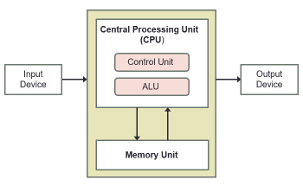
\includegraphics[width=0.4\textwidth]{vonNeumannArchi}
\end{figure}
The von Neumann architecture (also known as the \textit{Princeton
architecture}, or \textit{stored-program architecture}) describes a computer
consisting of:
\begin{itemize}
  \item Central Processing Unit (CPU) - Registers, A control unit containing an instruction register and program counter, An arithmetic/logic unit (ALU)
  \item Memory - Stores both program and data in random-access memory (RAM)
  \item I/O Devices
\end{itemize}

\subsubsection{Program Structure}
The form of a C Program typically looks like the following:
\begin{lstlisting}
preprocessor directives

structure types

function prototypes

main function header {
  declaration of variables
  executable statements
}

function definitions
\end{lstlisting}
\begin{figure}[h!]
  \centering
  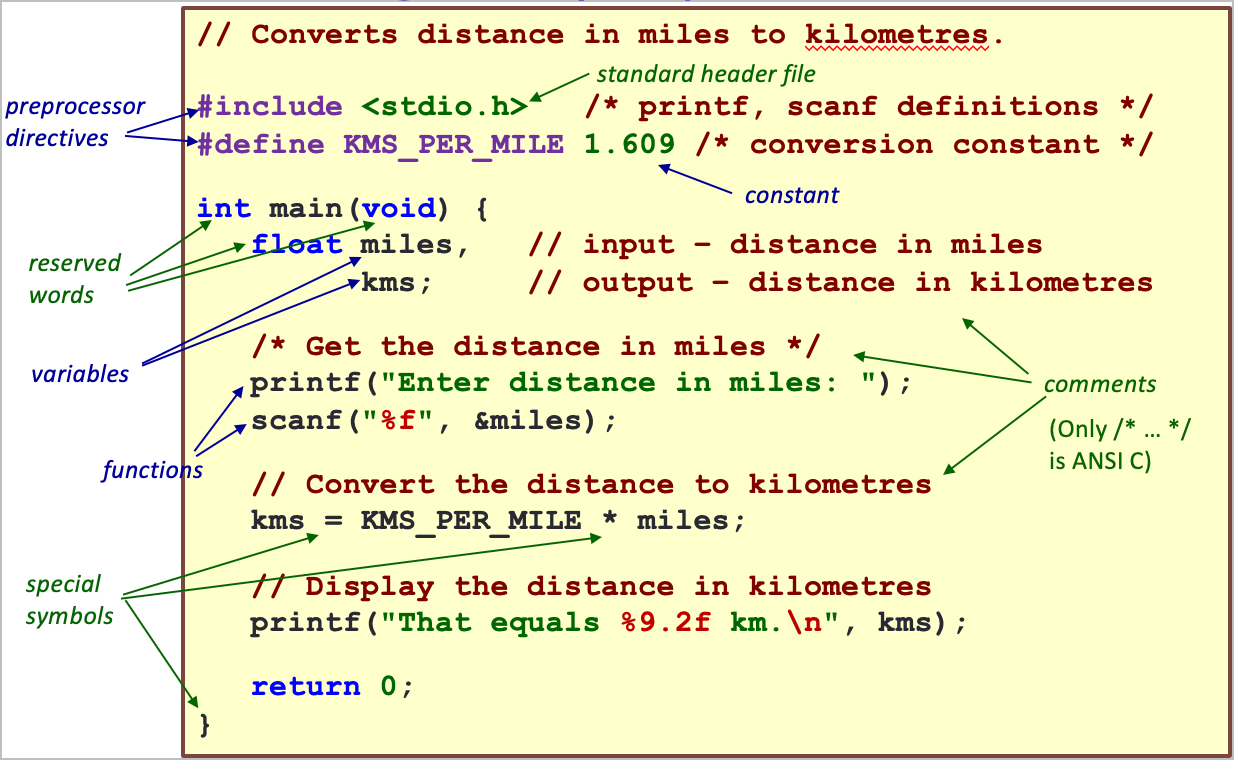
\includegraphics[width=0.8\textwidth]{cProgram}
\end{figure}

\begin{remark}
  The main function is obligatory in C. Typically, ``executable statements''
  consists 3 parts: \textit{Input data, Computation, Output Results}.
\end{remark}
\paragraph{Function Prototypes}
User-defined function prototypes are of the syntax
\begin{lstlisting}
  return_type function_name(parameter_type);
\end{lstlisting}
The names of parameters in the function prototype are optional and ignored by
the compiler.
\begin{remark}
 It is good practice to put function prototypes before the main function. 
\end{remark}
If no prototype is provided but the function is used, the compiler adds an
\textbf{implicit declaration} and returns a warning. The default return type is
assumed to be \verb|int|, and hence is almost always wrong.
\begin{example}
  The function parameter types may consist of arrays, strings and structs as well.
  \begin{lstlisting}
    int func(int *, int [], int);
  \end{lstlisting}
\end{example}

\subsection{Preprocessor Directives}
The C preprocessor provides the following:
\begin{itemize}
  \item Inclusion of header files:
    \begin{itemize}
      \item To use input/output functions such as \verb|scanf()| and
        \verb|printf()|: \verb|#include <stdio.h>| (compile with the \verb|-o|
        flag to specify output file)
      \item To use mathematical functions: \verb|#include <math.h>| and compile
        with the \verb|-lm| flag on sunfire.
      \item To use string functions: \verb|#include <string.h>|
    \end{itemize}
  \item Macro expansions:
    To define a macro for a constant value. Useful for declaring constants, to
    use all CAPS. \verb|#define PI 3.142| (without a semicolon, otherwise it
    will be included in the substitution).
  \item Conditional Compilation (Will not be introduced in CS2100)
\end{itemize}
\subsection{Input / Output}
We use format specifiers that serve as placeholders for values to be displayed
or read.
\vspace{2mm}

\centering
\begin{tabular}{c c c}
  \toprule
  Placeholder & Variable Type & Function Use \\
  \midrule
  \verb|%c| & char & printf / scanf \\
  \verb|%d| & int & printf / scanf \\
  \verb|%f| & float / double & printf \\
  \verb|%f| & float & scanf \\
  \verb|%lf|  & double & scanf \\
  \verb|%e| & float / double & printf (with scientific notation) \\
  \verb|%p| & address & printf (in hexadecimal)\\
  \bottomrule
\end{tabular}

\raggedright
\begin{example}[Format Specifiers]
  Examples of format specifiers used in \verb|printf()| are:
  \begin{itemize}
    \item \verb|%5d|: displays an integer in a width of 5, right justified.
    \item \verb|%8.3f|: displays a real number (float or double) in a width of 8,
      with 3 decimal places, right justified.
  \end{itemize}
  For \verb|scanf()|, format specifiers are used without indicating width or
  decimal places.
\end{example}

Additionally, we may use escape sequences in \verb|printf()| for certain special
effects or to display certain characters properly.
\vspace{2mm}

\centering
\begin{tabular}{c c c}
  \toprule
  Escape Sequence & Meaning & Result \\
  \midrule
  \verb|\n| & New line & Subsequent output appears on the next line \\
  \verb|\t| & Horizontal tab & Move to the next tab position on the current line \\
  \verb|\"| & Double quote & Displays a double quote " \\
  \verb|%%| & Percent & Dispalys a percent character \% \\
  \bottomrule
\end{tabular}

\raggedright
\subsection{Computation}
\subsubsection{Functions}
Computation in C is done through functions. A function body mainly composes of: 
\begin{itemize}
  \item \textit{Declaration statements} introducing an identifier and
    describing its type. It is required by the compiler to accept references to
    that identifier. Re-declaration is legal outside of class scope.
    \begin{remark}
      \verb|extern| can be used to import variables from another file. On
      variables, the variable is not allocated any memory. On functions, extern
      is the default and otherwise require \verb|static|. Similarly, using
      \verb|static| on a global variable ensures that it cannot be named
      outside of the current file. 
    \end{remark}
  \item \textit{Definition Statements} instantiating or implementing the identifiers. It
    is required by the linker to link references. It can be used in place of
    declarations.
  \item \textit{Executable statements} describing the processing on the memory
    cells.
\end{itemize}
\begin{remark}
  Using \verb|static| \textit{on a local variable} persists the value of the
  variable between function calls.
\end{remark}
\begin{remark}
  The special \verb|int main(void)| function is the entry point of the program.
\end{remark}

In C, function parameters are passed to the formal parameters through
\textit{pass-by-value}. That is, values of the actual parameters are copied to
the formal parameters.

\paragraph{Scope Rule}
\begin{definition}[Lexical Scoping]
  C uses \textit{lexical scoping}, also known as static scoping. That is, the
  compiler is able to deduce the scope of each variable at compile-time.
\end{definition}
Formal parameters and variables declared in the function are local to the
function. These local variables are only accessible in the function they are
declared. This is known as \textit{scope rule}. It is implemented as follows:
\begin{itemize}
  \item When a function is called, an activation record is created on the call
    stack, and memory is allocated for local parameters and variables (known as
    \textit{automatic variables}).
  \item When the function terminates, the activation record is removed, and
    memory allocated for the local parameters and variables is released.
\end{itemize}
In contrast to automatic variables, we have static variables that remain in
memory after the function is executed.

\subsubsection{Variables}
Data used in a program are stored in \textbf{variables}, identified by a name
(identifier), having a data type, containing a value which can be modified and
having an address (which varies from run to run).
\begin{remark}
  A variable is declared with a data type, and may be initialised during declaration
  \begin{lstlisting}
    int count = 3;
  \end{lstlisting}
  Without initialisation, the variable contains an unknown value (\textit{not
  necessarily zero}). We can use the \verb|-Wall| option during compilation to
  turn on warnings for missing initialisation.
\end{remark}
\begin{lstlisting}
int x;
scanf("%d", &x); // Refers to the (address of) the memory cell of x
printf("x equals %d\n", x) // Refers to the value in the variable x
\end{lstlisting}
C is a relatively strongly typed language, where every variable is to be
declared with a data type, but less so than Java or Pascal, as C supports
implicit type conversions and allows pointer values to be explicitly cast.
\subsubsection{Data Types}
In C, we have the basic data types (sizes in \textit{sunfire}):
\begin{itemize}
  \item int: $4\text{ bytes}; -2,147,483,648\ (-2^{31})\text{ to }+2,147,483,647\ (2^{31} – 1)$
  \item float: $4\text{ bytes};$ or double: $8\text{ bytes}$; May use
  scientific notation (e.g. \verb|1.5e-2|)
  \item char: Enclosed in a pair of single quotes.
\end{itemize}
The size of a type, or a variable, can be found using the \verb|sizeof()| function.\\
\begin{remark}
  With \verb|stdint.h|, we have more precise/unsigned integer types
  \verb|int8_t|, \verb|uint8_t|, \verb|int16_t|, \verb|uint16_t|,
  \verb|int32_t|, \verb|uint32_t|, \verb|int64_t|, \verb|uint64_t|, which can
  be printed with \verb|inttypes.h|.
\end{remark}
\subsubsection{User-defined Identifiers}
To define functions, or declare the use of variables, the user is required to
define the identifier as the name of a variable or function. It is obligatory
to follow the following rules:
\begin{itemize}
  \item Consists of letters (a-z, A-Z), digits (0-9), and underscores (\_)
    but cannot begin with a digit.
  \item Cannot be a reserved word. See \url{http://c.ihypress.ca/reserved.html}
    for a complete list.
\end{itemize}
In addition, it is recommended (while not obligatory) to follow these restrictions:
\begin{itemize}
  \item Begins with a lowercase letter, except constants which we identify in ALL CAPS.
  \item Avoids standard identifiers (names of common functions) such as
  \verb|printf|, \verb|scanf|.
  \begin{lstlisting}
    # include <stdio.h>
    int printf=5 // No issue, if printf() is not used
    printf("Hello world!") // Compile time error thrown from this line.
  \end{lstlisting}
\end{itemize}
\subsubsection{Assignment Statements}
Executable statements, in general, are I/O statements or computational and
assignment statements. Assignment statements store a value in a variable:
\verb|lvalue = 30;|.
\begin{remark}
  \verb|lvalue| must be assignable. That is, \verb|32 = a| (not a variable)
  and \verb|a + b = c| (an expression) are not assignable and throws the
  compilation error "lvalue required as left operand of assignment".
\end{remark}
Additionally, assignment can be cascaded, with associativity from right to left:

\centering
\verb|a = b = c = 1 + 2| $\equiv$ \verb|a = (b = (c = 1 + 2))|

\raggedright
In C, the assignment statement has the side effect of returning the value of
the expression. This allows the cascading of assignment as shown, but also
allows statements such as \verb|a = 5 + (b = 10)|.
\subsubsection{Operations}
\begin{tabular}{c c c}
  \toprule
  Operator & Operator & Associativity \\
  \midrule
  Primary Expression Operators & \verb|()  []  .  ->  expr++  expr--| & Left to right \\
  Unary Operators & \verb|* & + ! ~ - ++expr --expr (typecast) sizeof| & Right to left \\
  \multirow{6}{8em}{Binary Operators} & \verb|*  /  %| & \multirow{6}{5.3em}{Left to right} \\
   & \verb|+  -| &  \\
   & \verb|<  >  <=  >=| &  \\
   & \verb|==  !=| &  \\
   & \verb|&&| &  \\
   & \verb$||$ &  \\
  Ternary Operator & \verb|predicate ? consequent : alternative| & Right to left\\
  Assignment Operators & \verb|=  +=  -=  *=  /=  %=| & Right to left\\
  \bottomrule
\end{tabular}
\begin{remark}
  In C, the operator \verb|%| calculates the remainder \verb|a%b| as follows:
  \[\left(a/b\right)*b+a\ \%\ b=a.\] 
\end{remark}
\begin{remark}
  There is no Boolean type in ANSI C. We use \verb|0| to represent
  \textit{false}, and any other value to represent \text{true}.
\end{remark}
Mixed-typed arithmetic operations:
\begin{multicols}{2}
\begin{itemize}
  \item \verb|int  m = 10/4; // m = 2|
  \item \verb|float p = 10/4; // p = 2.0|
  \item \verb|int n = 10/4.0; // n = 2|
  \item \verb|float q = 10/4.0; // q = 2.5|
\end{itemize}
\begin{itemize}
  \item \verb|int r = -10/4.0; // r = -2|
  \item \verb|float pp = (float) aa/4; // pp = 1.5|
  \item \verb|int nn = (int) ff / aa; // nn = 2|
  \item \verb|int qq = (float) (aa/4); // qq = 1.0|
\end{itemize}
\end{multicols}

\subsubsection{Math Library}
With inclusion of the \verb|<math.h>| library, compiled with the \verb|-lm|
option, we are able to use the following common math functions:
\begin{multicols}{2}
  \begin{itemize}
    \item \verb|int abs(int x)|
    \item \verb|double fabs(double x)|
    \item \verb|double ceil(double x)|
    \item \verb|double floor(double x)|
    \item \verb|double exp(double x)|
    \item \verb|double pow(double x, double y)|
  \end{itemize}
  \begin{itemize}
    \item \verb|double log(double x)|
    \item \verb|double log10(double x)|
    \item \verb|double sqrt(double x)|
    \item \verb|double cos(double x)| (radians)
    \item \verb|double sin(double x)| (radians)
    \item \verb|double tan(double x)| (radians)
  \end{itemize}
\end{multicols}

\subsection{Pointers}
Using pointers, we are able to directly manipulate memory contents. We are able
to modify the value of variables outside of a function's scope within the
function, by passing in the pointer into the function.
\begin{definition}[Pointer]
  A variable that contains the address of another variable is known as a
  pointer, or a pointer variable.
\end{definition}
To work with addresses, we have the unary \textit{address operator} \verb|&| to
obtain the address of a given variable and \textit{dereferencing/indirection
operator} \verb|*| to access the value of a given address.

To declare a pointer to a variable of \verb|type|, we use the syntax
\begin{lstlisting}
  type *variable_ptr; // Convention to name pointer with suffix _ptr or _p
\end{lstlisting}

\begin{remark}
  Using the address of an uninitialised variable is well-defined behaviour, but using
  a uninitialised pointer is undefined behaviour.
  \begin{lstlisting}
    char x;
    printf("%p\n", &x); // Prints address of x
    char *y;
    printf("%p\n", y); // Issues warning
  \end{lstlisting}
\end{remark}

Using pointers can lead to issues relating to correctness and security, such as:
\begin{itemize}
  \item \textbf{Aliasing}: When two pointers point to the same object and we
    might not be able to tell.
  \item \textbf{Invalid/NULL pointer dereferencing}: Inability to check validity of a pointer.
  \item \textbf{Dangling Pointers}: When the memory object being pointed has
    been freed/is no longer available.
\end{itemize}

\begin{remark}
  Since all pointers have the same size and can point to the storage of no
  type, we can create a \textit{generic pointer}
  \[\verb|void *ptr|.\]
   This allows for a pointer that refers to a value that has unknown type, or
   several possible types, and is often used as a parameter of generic
   functions. They should be \textit{typecast} before valid usage.
\end{remark}

\subsubsection{Pointer Arithmetic}
When a pointer is incremented, the address is incremented by the size of the
pointer's type. For instance, a int pointer will be incremented by 4 bytes,
while a char pointer will be incremented by 1 byte.

\subsubsection{Dynamic Storage Allocation}
During runtime, we may allocate storage by using the \verb|void *malloc(size)|
system call. It exists as a pair to the \verb|free((void *)ptr)| system call to
free the pointer. However, this requires caution as it may result in dangling
pointers and hence undefined behaviour.

\subsection{Arrays, Strings and Structures}
To further organise data beyond the basic data types, with more logical
representations and greater ease of manipulations, we may use arrays, strings
and structs in C.
\subsubsection{Arrays}
Arrays are defined by the \textit{element type, array name and maximum size}. They
occupy \textbf{contiguous} memory locations and are accessed through indexing.
The array name itself is a pointer, which refers to the address of the
first element of that array. That is,
\[\verb|arr|\equiv \verb|&arr[0]|.\] 
Additionally, it is a \textbf{fixed pointer}. It is hence \textit{illegal} to
alter the value of this variable.
\begin{remark}
  Arrays can only be initialised \textit{at the time of declaration}.
  \begin{lstlisting}
    int arr[3] = {1, 2, 3};
  \end{lstlisting}
\end{remark}
As a function parameter, arrays can be taken as both a pointer or an array.
\begin{lstlisting}
  int sumArray(int *arr, int size) { ... }
  int sumArray(int arr[], int size) { ... }
\end{lstlisting}
Since the array name is a pointer, the function is able to modify the contents
of the passed array.

\paragraph{Multi-Dimensional Arrays} Given a array of type \verb|T|:
\[\verb|T a[D1][D2]|\ldots\verb|[Dn];|,\] 
where \verb|Dj| is the size of dimension $j$. $A_0$ is the address of the first
element \verb|a[0][0]|\ldots\verb|[0]|, and $S$ the size of each element of \verb|T|. We have
the address of the element \verb|a[i1][i2]|\ldots\verb|[in]| given by
\[A_0+S\times \left( \left( \left( \left( \verb|i1|\times \verb|D2|+\verb|i2| \right) \times \verb|D3|+\verb|i3| \right)\cdots \right)\times \verb|Dn|+\verb|in| \right) .\] 

\subsubsection{Strings}
A string is an \textit{array of characters terminated by a null character}
`\textbackslash0'. It can be defined by assigning each character to an array of
characters, or initialising the string directly:
\begin{multicols}{2}
  \begin{lstlisting}
    char str[6];
    str[0] = 'e';
    str[1] = 'g';
    str[2] = 'g';
    str[3] = '\0';
  \end{lstlisting}
  \begin{lstlisting}
    char str[] = "egg";
    char str[] = {'e', 'g', 'g', '\0'}
  \end{lstlisting}
  \vfill\null
\end{multicols}
Similarly, the string itself is a pointer referring to the address of the first
character of the string.

\begin{remark}
  We may include \verb|<string.h>| for string manipulation functions:
    \begin{itemize}
      \item \verb|int strlen(char *s)|
      \item \verb|int strcmp(char *s1, char *s2)|: s1 $-$ s2
      \item \verb|int strncmp(char *s1, char *s2, int n)|
      \item \verb|char *strcpy(char *s1, char *s2)|: s2 $\to$ s1
      \item \verb|char *strncpy(char *s1, char *s2, int n)|
    \end{itemize}
  It is typically preferred to use the functions with predefined maximum
  lengths $n$ to prevent exploits.
\end{remark}

\paragraph{String I/O}
In addition to the usual functions \verb|scanf("%s", str)| and
\verb|printf("%s\n", str)|,
strings can be read and printed using the\\
\centering
\verb|fgets(str, size, stdin)| and \verb|puts(str)| functions.\\
\raggedright
\begin{remark}
  \verb|fgets| also reads in the newline character, which may need to be
  replaced with the null character.
\end{remark}

\subsubsection{Structures}
\textit{Structure types} allow for grouping of heterogeneous members, and even
of other groups themselves.
\begin{lstlisting}
  typedef struct {
    type_1 x;
    type_2 y;
  } type_name;
\end{lstlisting}
\begin{remark}
  Structure types are definitions of types, not a declaration of a variable. No
  memory is allocated until a variable is declared.
\end{remark}
\begin{example}[Nested Structure Variable]
  Structure variables can then be initialised similarly to array
  initialisation, and members accessed using the dot \verb|.| operator:
  \begin{multicols}{2}
    \begin{lstlisting}
    typedef struct {
      int day, month, year;
    } date_t;

    typedef struct {
      int cardNum;
      date_t expiry;
    } card_t;
    \end{lstlisting}
    \begin{lstlisting}
      card_t card = {12345, {7, 10, 2025}};
      card.expiry.year = 2026;
      scanf("%d", &card.cardNum);

      // Assignments with structures are legal.
      card_t card_1 = {1, {1, 1, 1}};
      card_1 = card;
    \end{lstlisting}
    \vfill\null
  \end{multicols}
\end{example}
\begin{remark}
  Due to \textit{pass-by-value}, structures, when passed into a function, are
  \textbf{copied} into the formal parameters.
  To modify structure variables, the address of the variable is passed instead.
\end{remark}
We define the arrow operator \verb|->| as a ``shortcut'' syntax to access
members of a pointer to a structure variable:
\[\verb|(*struct_ptr).member|\equiv\verb|struct_ptr->member|\] 

\subsubsection{Unions and Enum}
Unions are a special type of structures in which the fields occupy the same
memory storage (that of the field requiring the greatest memory storage). That
is, only one of the fields can be defined in a union for defined behaviour.

Enum is a similar type that represents a group of integer constants, to
constrain options and choices.

\section{Data Representation and Number Systems}
Data is internally represented as a sequence of bits (binary digits). How it is
represented depends on the data type, and certain bit strings can have
different values when taken as different data types.
\begin{definition}[Units of Data Representation]
  Each \textbf{byte} is 8 bits, each \textbf{nibble} is 4 bits, and each
  \textbf{word} is multiple bytes depending on computer architecture. For
  example, 64-bit architecture uses 8 bytes and 32-bit architecture uses 4
  bytes as the word size.
\end{definition}
$N$ bits can represent up to $2^{N}$ values. To represent $M$ values,
$\lceil\log_2 M\rceil$ bits are required. 
\subsection{Number Systems}
We consider a weighted-positional number system, in the usual \textit{base} (or
radix) 10.
\begin{definition}[Weighted-Positional Number System]
  We consider a weighted-positional number system, in \textit{base} (or \textit{radix}) R:\@
  Then we have the \textit{symbols}/\textit{digits}$=\left\{ 0,1,2,\ldots,R-1 \right\}$
  and each position has a weight of power of R.
  \[{\left( a_{n}a_{n-1}\cdots a_0.f_1f_2\cdots f_m \right)}_R=\]
  \[(a_{n}\times 10^{n})+(a_{n-1}\times 10^{n-1})+\cdots+(a_0\times 10^{0})+(f_1\times 10^{-1})+(f_2\times 10^{-2})+\cdots+(f_m\times 10^{-m})\]
\end{definition}
\begin{notation}[Number Systems Notations]
  In certain programming languages, we can specify certain bases of numbers as follows:
  \begin{multicols}{3}
    \begin{itemize}
      \item In \verb|C|:
      \begin{itemize}
        \item Prefix \verb|0| for octal
        \item Prefix \verb|0x| for hexadecimal
      \end{itemize}
      \vfill\null%
      \columnbreak%
    \item In \verb|QTSpim|:
      \begin{itemize}
        \item Prefix \verb|0x| for hexadecimal
      \end{itemize}
      \vfill\null%
      \columnbreak%
    \item In \verb|Verilog|:
      \begin{itemize}
        \item Prefix \verb|8'b| for binary
        \item Prefix \verb|8'h| for hexadecimal
        \item Prefix \verb|8'd| for decimal
      \end{itemize}
    \end{itemize}
  \end{multicols}
\end{notation}
\subsubsection{Conversion}
To convert any base-R number to decimal, we sum the symbols, with each scaled
by a weight of power of R corresponding to its position.
\begin{example}[From Base-5 to Decimal]
  \[341.24_5=3\times 5^{2}+4\times 5^{1}+1\times 5^{0}+2\times 5^{-1}+4\times 5^{-2}=96.56_{10}.\]
\end{example}
To convert a whole decimal number to any base-R number, we use
\textbf{successive division by $R$} until the quotient is 0. Each remainder
forms the answer, with the first remainder as the \textit{Least Significant
Bit} (LSB) and the last as the \textit{Most Significant Bit} (MSB).
\begin{example}[Decimal Whole Number to Binary]
  \[43_{10}=(1 \bmod 2)(2 \bmod 2)(5 \bmod 2)(10 \bmod 2)(21 \bmod 2)(43 \bmod 2)=101011_2.\] 
\end{example}
To convert a decimal fraction to any base-R number, we use \textbf{repeated
multiplication by $R$}, until the fractional product is 0 or the required
precision is achieved. The \textit{carries} produce the answer, with the first
carry as the MSB and the last as the LSB.%
\begin{example}[Decimal Fraction to Binary]
  \[0.3125_{10}=(0.3125\times 2\bmod 1)(0.625\times 2\bmod 1)(0.25 \times 2\bmod 1)(0.5\times 2\bmod 1)=0.0101.\] 
\end{example}
In general, to convert between non-decimal bases $R$ and $S$, we convert first
to decimal and then to the desired base.
\begin{remark}
  However, we may convert between binary, octal, and hexadecimal by grouping
  symbols together or expanding into multiple symbols directly.
\end{remark}

\subsection{Data Representation}
\subsubsection{Character Representation}
ASCII code and Unicode is used to represent characters. Each character is
$8$ bits in ASCII, consisting $7$ bits and $1$ parity bit. Hence characters take
ASCII code values from $0$ to $127$.
\begin{figure}[h!]
  \centering
  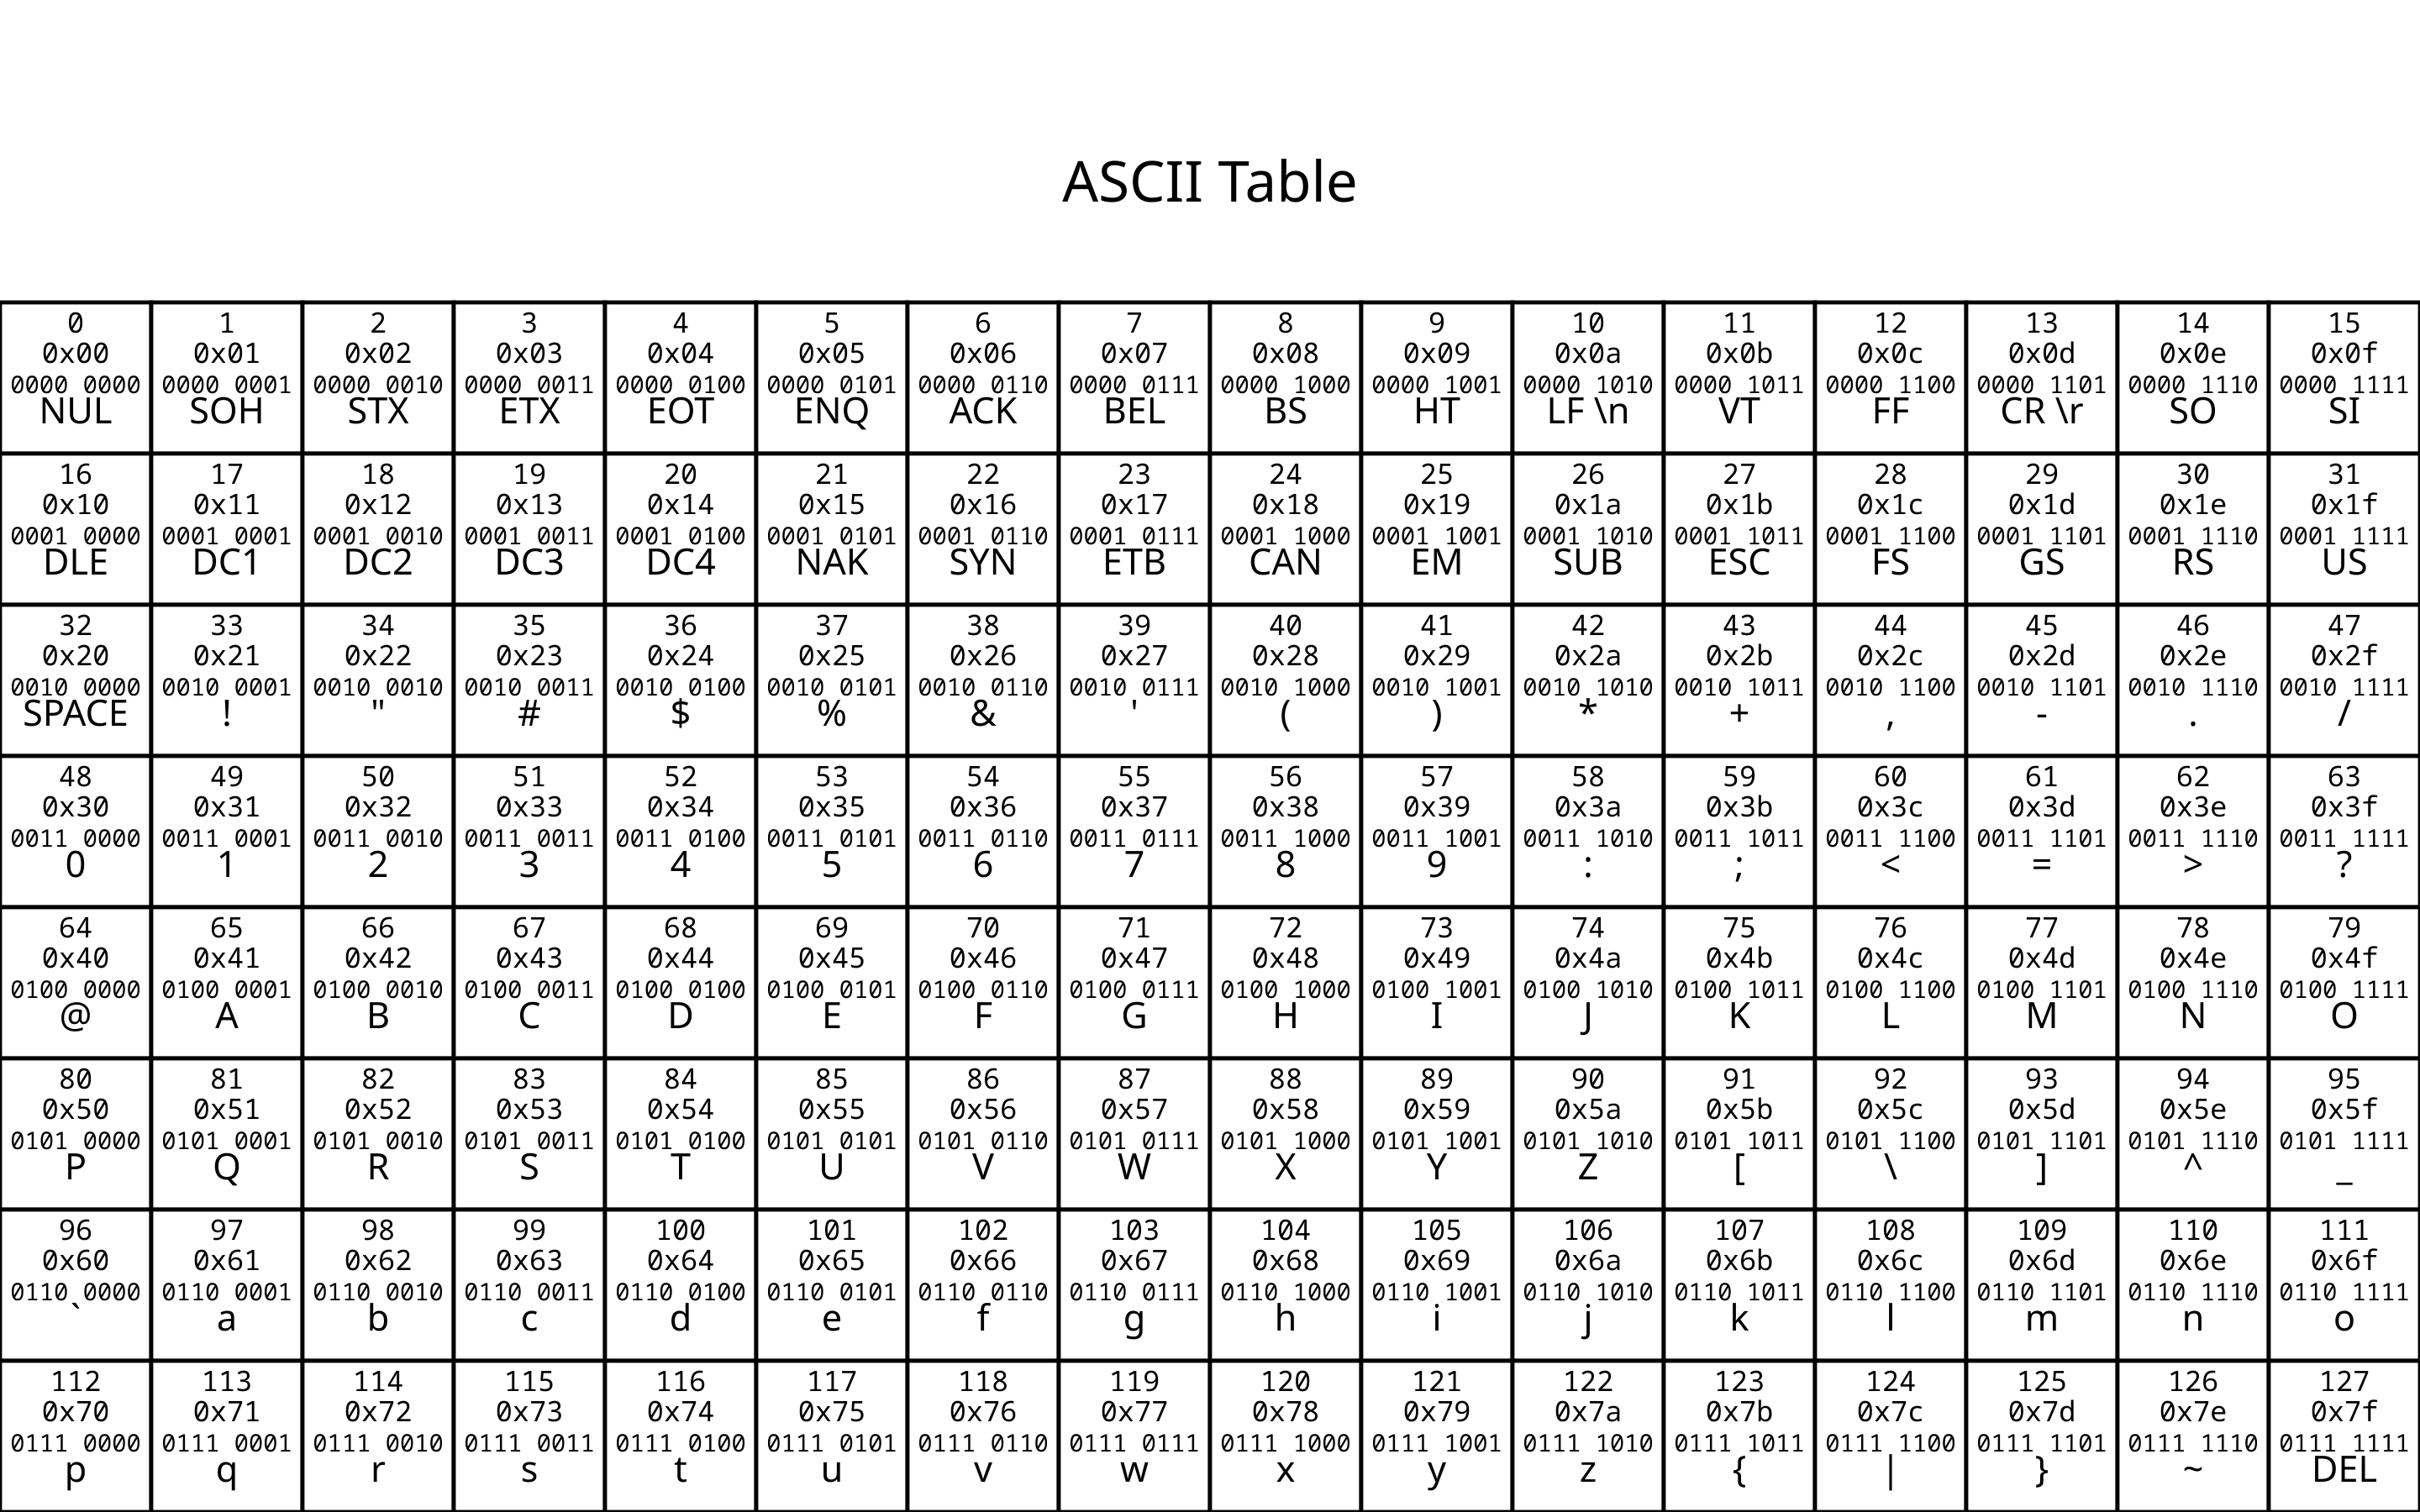
\includegraphics[width=0.8\textwidth]{ASCII_Table.png}
\end{figure}

\subsubsection{Integer Representation}
Numbers in C can either be unsigned or signed.\ \textit{Unsigned Numbers} can
only take non-negative values. In this case, the range of values it can take
would be from $0$ to $2^{n}-1$, where $n$ is the number of bits used.
\textit{Signed Numbers} can take both positive and negative values. However,
with the same number of bits, the range of values would hence be smaller (since
information on the sign has to be stored with a bit). There are three common
representations, namely \textbf{Sign-and-Magnitude}, \textbf{1s Complement},
and \textbf{2s Complement}. 

\paragraph{Sign-and-Magnitude}
We may represent a negative number using the MSB as a `sign bit', with $0$ for $+$ and
$1$ for $-$. We hence have, for $8$-bit integers:
In general, the range is $-2^{n-1}+1$ to $+2^{n-1}-1$ for a $n$-bit integer. We
negate a number by simply inverting the sign bit.
\[\text{Range: }11111111_2=-127_{10}\text{ to }01111111_2=+127_{10}\]
\[\text{Zeros: }00000000=+0_{10}\text{ and }10000000=-0_{10}\]

\paragraph{1s Complement}
Given a positive number $x$, its additive inverse is given in 1s-complement representation by
\[-x=2^{n}-x-1.\]
\begin{example}[$12_{10}$]
  With an $8$-bit number $00001100_2$, its negated value expressed in 1s-complement is:
  \begin{align*}
    -{\left( 00001100 \right)}_2&=(2^{8}-12-1)\\
                                &=243\\
                                &={11110011}_{1s}
  \end{align*}
\end{example}
In general, the range is $-2^{n-1}+1$ to $+2^{n-1}-1$ for a $n$-bit integer. We
negate a number by inverting all of its bits. The MSB still represents the sign
of the integer.
\[\text{Range: }10000000_{1s}=-127_{10}\text{ to }01111111_{1s}=+127_{10}\]
\[\text{Zeros: }00000000=+0_{10}\text{ and }11111111=-0_{10}\]
When performing \textbf{addition of integers in 1s complement}, add the `carry out' of
the MSB to the LSB\@. Overflow occurs if the result is opposite sign of $A$ and
$B$.

\paragraph{2s Complement}
Given a positive number $x$, its additive inverse is given in  2s-complement representation by
\[-x=2^{n}-x.\] 
\begin{example}[$12_{10}$]
  With an $8$-bit number $00001100_2$, its negated value expressed in 2s-complement is:
  \begin{align*}
    -{\left( 00001100 \right)}_2&=(2^{8}-12)\\
                                &=244\\
                                &={11110100}_{2s}
  \end{align*}
\end{example}
In general, the range is $-2^{n-1}$ to $+2^{n-1}-1$ for a $n$-bit integer. We
negate a number by inverting all of its bits, then add $1$. The MSB still represents the sign
of the integer.
\[\text{Range: }10000000_{1s}=-128_{10}\text{ to }01111111_{1s}=+127_{10}\]
\[\text{Zeros: }00000000=+0_{10}\text{ and }11111111=-0_{10}\]
When performing \textbf{addition of integers in 2s complement}, the carry out of the MSB is ignored.
Overflow occurs if the `carry in' and the `carry out' of the
MSB is different, or if the result is opposite sign of $A$ and $B$.
\begin{definition}[Sign Extension]
  To convert a $n$-bit \textbf{signed} integer to a $m$-bit signed integer
  (where $m>n$), we copy the MSB $m-n$ times to the left of the $n$-bit number.
  That is, we copy the `sign' bit of the integer.  This is
  \textit{value-preserving} only for 2s complement.
\end{definition}

\paragraph{Excess-$k$ Representation} 
Given a number in excess-$k$ representation, we may obtain its value in decimal
by taking the number as binary, and then subtracting $k$.
\begin{example}[Excess-$8$]
  For $4$-bit numbers, excess-$8$ is as shown below:

\centering
\begin{tabular}{c c c c c c c c c}
  \toprule
  Excess-$8$ Representation & $0000$ & $0001$ & $0010$ & $0011$ & $0100$ & $0101$ & $0110$ & $0111$ \\
  \midrule
                           Value & $-8$ & $-7$ & $-6$ & $-5$ & $-4$ & $-3$ & $-2$ & $-1$\\
                           \bottomrule
\end{tabular}
\begin{tabular}{c c c c c c c c c}
  \toprule
  Excess-$8$ Representation& $1000$ & $1001$ & $1010$ & $1011$ & $1100$ & $1101$ & $1110$ & $1111$\\
  \midrule
  Value & $0$ & $1$ & $2$ & $3$ & $4$ & $5$ & $6$ & $7$\\
  \bottomrule
\end{tabular}
\end{example}
\raggedright%

\subsection{Real Number Representation}
In \textbf{fixed-point representation}, we fix the number of bits allocated for
the integer and fractional parts. 
\begin{figure}[h!]
  \centering
  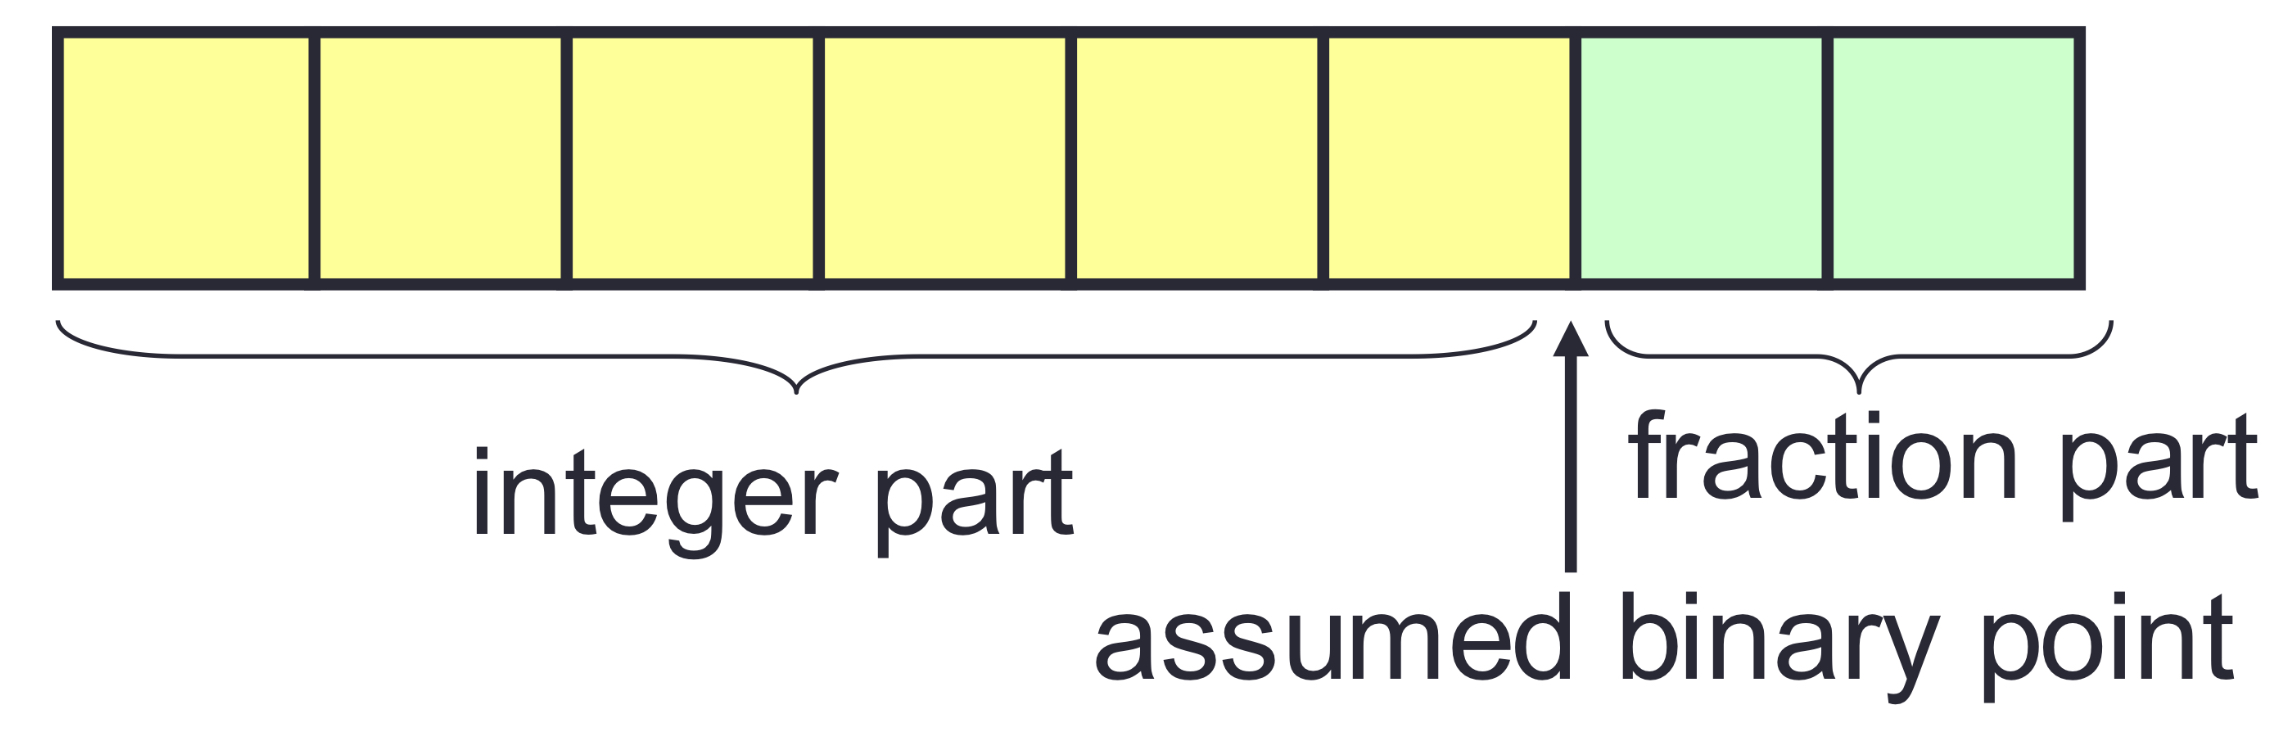
\includegraphics[width=0.4\textwidth]{fixedPoint.jpeg}
\end{figure}\\
We extend the limited range of fixed-point representation with
\textbf{floating-point representation}, allowing us to represent very large or
very small numbers.
\paragraph{IEEE 754 Floating-Point Representation}
The floating-point representation comprises 3 components: \textit{sign},
\textit{exponent}, and \textit{mantissa} (fraction).
\begin{itemize}
  \item Single-precision (32 bits): 1-bit sign, 8-bit exponent in excess-127, 23-bit mantissa
  \item Double-precision (64 bits): 1-bit sign, 11-bit exponent in excess-1023, 52-bit mantissa
\end{itemize}
The sign bit has $0$ for $+$, and $1$ for $-$. The exponent has an implicit
base $2$, and is stored in excess representation, whereas the mantissa is normalised
with an implicit leading bit 1. That is, the mantissa only stores the bits
after the binary point.
\[v={\left( -1 \right)} ^{sign}\times 1.fraction\times 2^{exponent-bias}.\] 
\begin{example}[$-6.5_{10}$]
  To represent a given value, we first convert into binary, and normalise the mantissa:
  \[-6.5_{10}=-110.1_2=-1.101_2\times 2^{2}.\]
  We hence have the sign bit $=1$, exponent
  $=2_{10}=10000001_{\text{excess-}127}$, mantissa $=10100000000000000000000$.
\end{example}
\begin{definition}[Underflow and Overflow]
  With the discrete representation of numbers, we have numbers that are
  non-representable on the number line, as shown:
  \begin{figure}[h!]
    \centering
    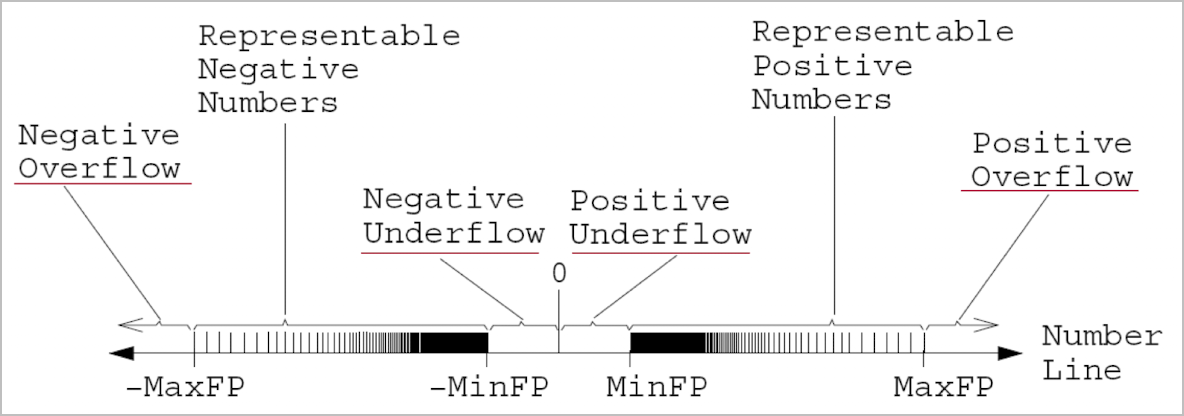
\includegraphics[width=0.5\textwidth]{floatingUnderOverflow.png}
  \end{figure}
  As such, associativity is not preserved, since 
  \[\left( A \cdot B \right) \cdot C=round{\left( round{\left( A \cdot B \right)} \cdot C \right) }.\]
\end{definition}
Depending on implementation, rounding can be to the nearest (default), towards
zero, towards positive infinity, or negative infinity. The operation is done
with 3 extra bits (guard, round, sticky), and then rounded to the nearest
representable number.

\section{Instruction Set Architecture}
\textbf{Instruction Set Architecture} (ISA) is an abstraction on the interface
between the hardware and low-level software. It abstracts the functionality
of the processor, such that
\begin{itemize}
  \item Programmers are aware of functionality available from machine code
  \item Computer Designers can design functionality independent of the hardware
\end{itemize}
\begin{figure}[h!]
  \centering
  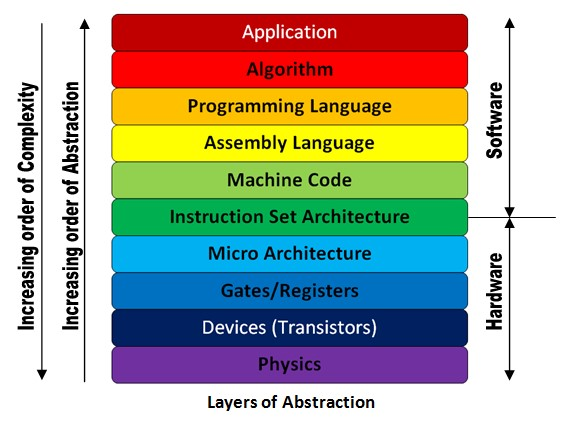
\includegraphics[width=0.4\textwidth]{isa.jpg}
\end{figure}
\subsection{ISA Design}
We have two major design philosophies for ISA:
\vspace{2mm}

\centering
\begin{tabular}{c c}
  \toprule
  Complex Instruction Set Computer (CISC) & \textbf{Reduced Instruction Set Computer (RISC)} \\
  \midrule
  Complex operations with single instruction & Simple and small instruction set \\
  Smaller program size & Larger program size \\
  No room for hardware optimisation & Easier to build/optimise hardware\\
                                    & Burden on software to implement high-level statements\\
  \bottomrule
\end{tabular}

\vspace{2mm}
\raggedright
ISA Design comprises 5 main concepts:
\begin{enumerate}
  \item \textbf{Data Storage}: Storage Architecture
  \item \textbf{Memory Addressing Nodes}
  \item \textbf{Operations in the Instruction Set}
  \item \textbf{Instruction Formats}: Instruction Length, Fields
  \item \textbf{Encoding the Instruction Set}
\end{enumerate}

\subsubsection{Data Storage}
In data storage, we concern ourselves with storing the operands, the results,
and how the operands are specified. We have the common storage architecture
designs:
\begin{figure}[h!]
  \centering
  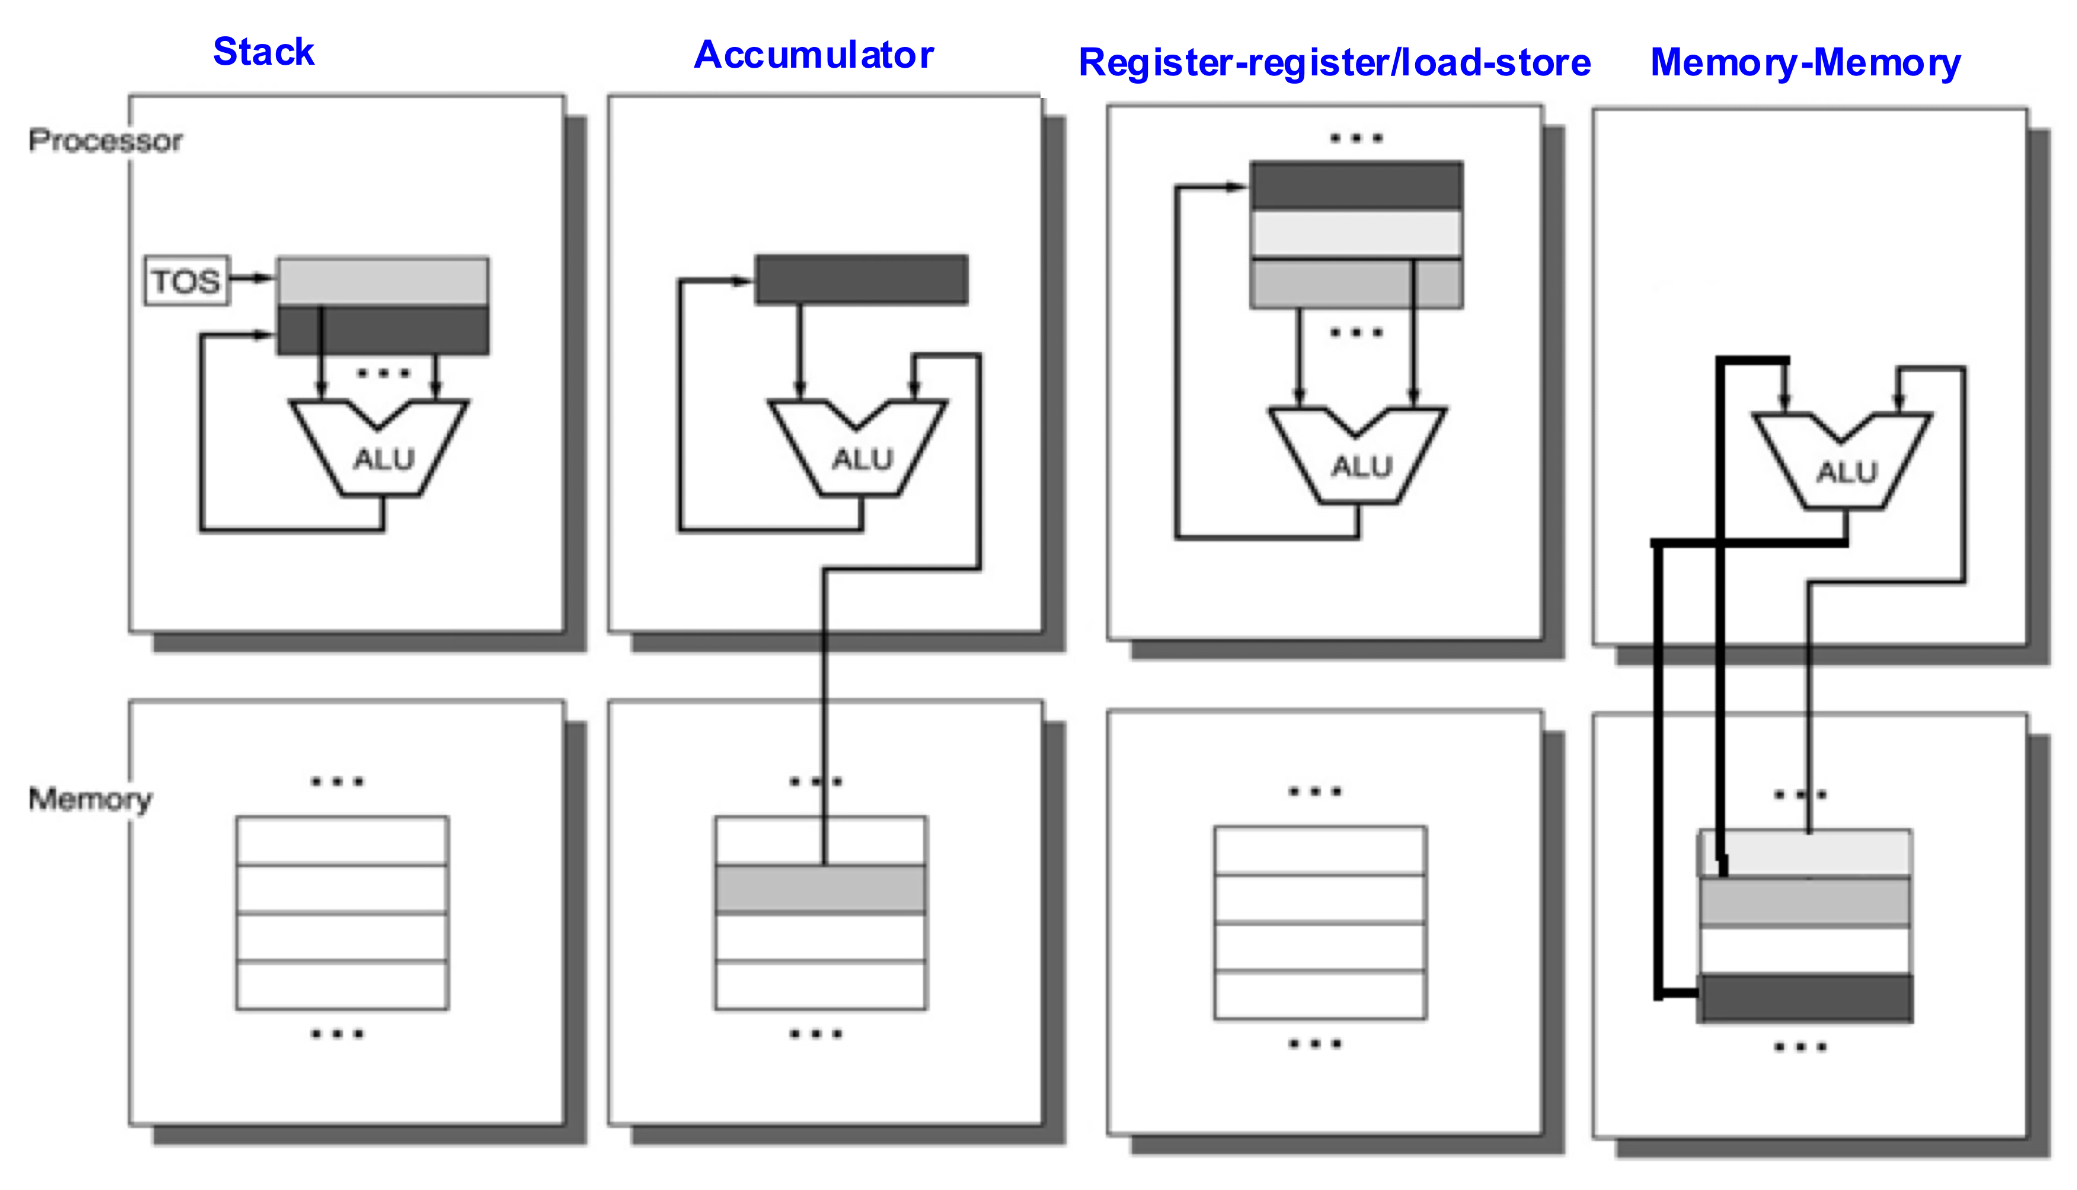
\includegraphics[width=0.65\textwidth]{storageArchi.jpeg}
\end{figure}
\begin{itemize}
  \item \textit{Stack Architecture}: Operands are implicitly on top of a stack
  \item \textit{Accumulator Architecture}: One operand is implicitly in a special
    register known as the accumulator (IBM 701, DEC PDP-8)
  \item \textit{General-Purpose Register Architecture}: Operands are explicit. Most common design.
      \begin{itemize}
        \item \textit{Register-Memory Architecture}: Exactly one operand is in
          memory (Motorola 68000, Intel 80386)
        \item \textit{Register-Register (Load-Store) Architecture}: Both
          operands are in registers (\textbf{MIPS}, DEC Alpha)
      \end{itemize}
  \item \textit{Memory-memory Architecture}: All operands are in memory. (DEC VAX)
\end{itemize}

\subsubsection{Memory Addressing Mode}
Given a $k$-bit address, we have an address space ($0$ to $2^{32}-1$) of size
$2^{k}$, and each memory transfer consists of one word of $n$ bits. In
register-register architecture, the memory addressing node consists of the
\textit{Memory Address Register}, \textit{Memory Data Register} which are used
by the address/data bus and the control lines to load/store data.
\paragraph{Endianness} Within a multi-byte word (say 4), the most significant
byte can be stored in the lowest address. That is, we construct the byte by
reading from memory sequentially. This is known as \textbf{big-endian}. On the
contrary, \textbf{little-endian} is the case when the least significant byte is
stored in the lowest address.
\begin{remark}
  Each byte itself is not reversed.
\end{remark}
\paragraph{Addressing Mode} For storage architectures involving explicit
operands, there are different methods of specification in the assembly
language.
\begin{example}[MIPS]
  There are 3 addressing modes in MIPS:
  \begin{itemize}
    \item \textit{Register}: Operands are specified by the register containing
    the value (\verb|add $t1, $t2, $t3|)
    \item \textit{Immediate}: Operand is specified directly in the instruction
    with its value (\verb|addi $t1, $t2, 3|)
    \item \textit{Displacement}: Operand is in memory with address calculated
    as Base $+$ Offset (\verb|lw $t1, 20($t2)|)
  \end{itemize}
\end{example}
\begin{example}[Other Addressing Modes]
  There exist other addressing modes:
  \begin{itemize}
    \item \textit{Register Indirect}: Operand is specified with a register storing
      its address
    \item \textit{Indexed/Base}: Operand is in memory with address calculated
      with Base $+$ Offset, each stored in a register
    \item \textit{Direct/Absolute}: Operand is specified directly in the instruction
      with its address
    \item \textit{Memory Indirect}: Operand is specified with a register
      containing a address to its address.
    \item \textit{Auto-increment}: Operand is written into the destination,
      then incremented
    \item \textit{Auto-decrement}: Operand is decremented, then written into
      the destination
    \item \textit{Scaled}: Operand is in memory with address calculated as Base
      $+$ Offset + Index $\times $ Scaling\_Factor
  \end{itemize}
\end{example}
\subsubsection{Operations in the Instruction Set}
Instructions are optimised based on usage frequency --- the speeds for load,
conditional branch, compare and store instructions are optimised (potentially
at the cost of other instructions).
\begin{figure}[h!]
  \centering
  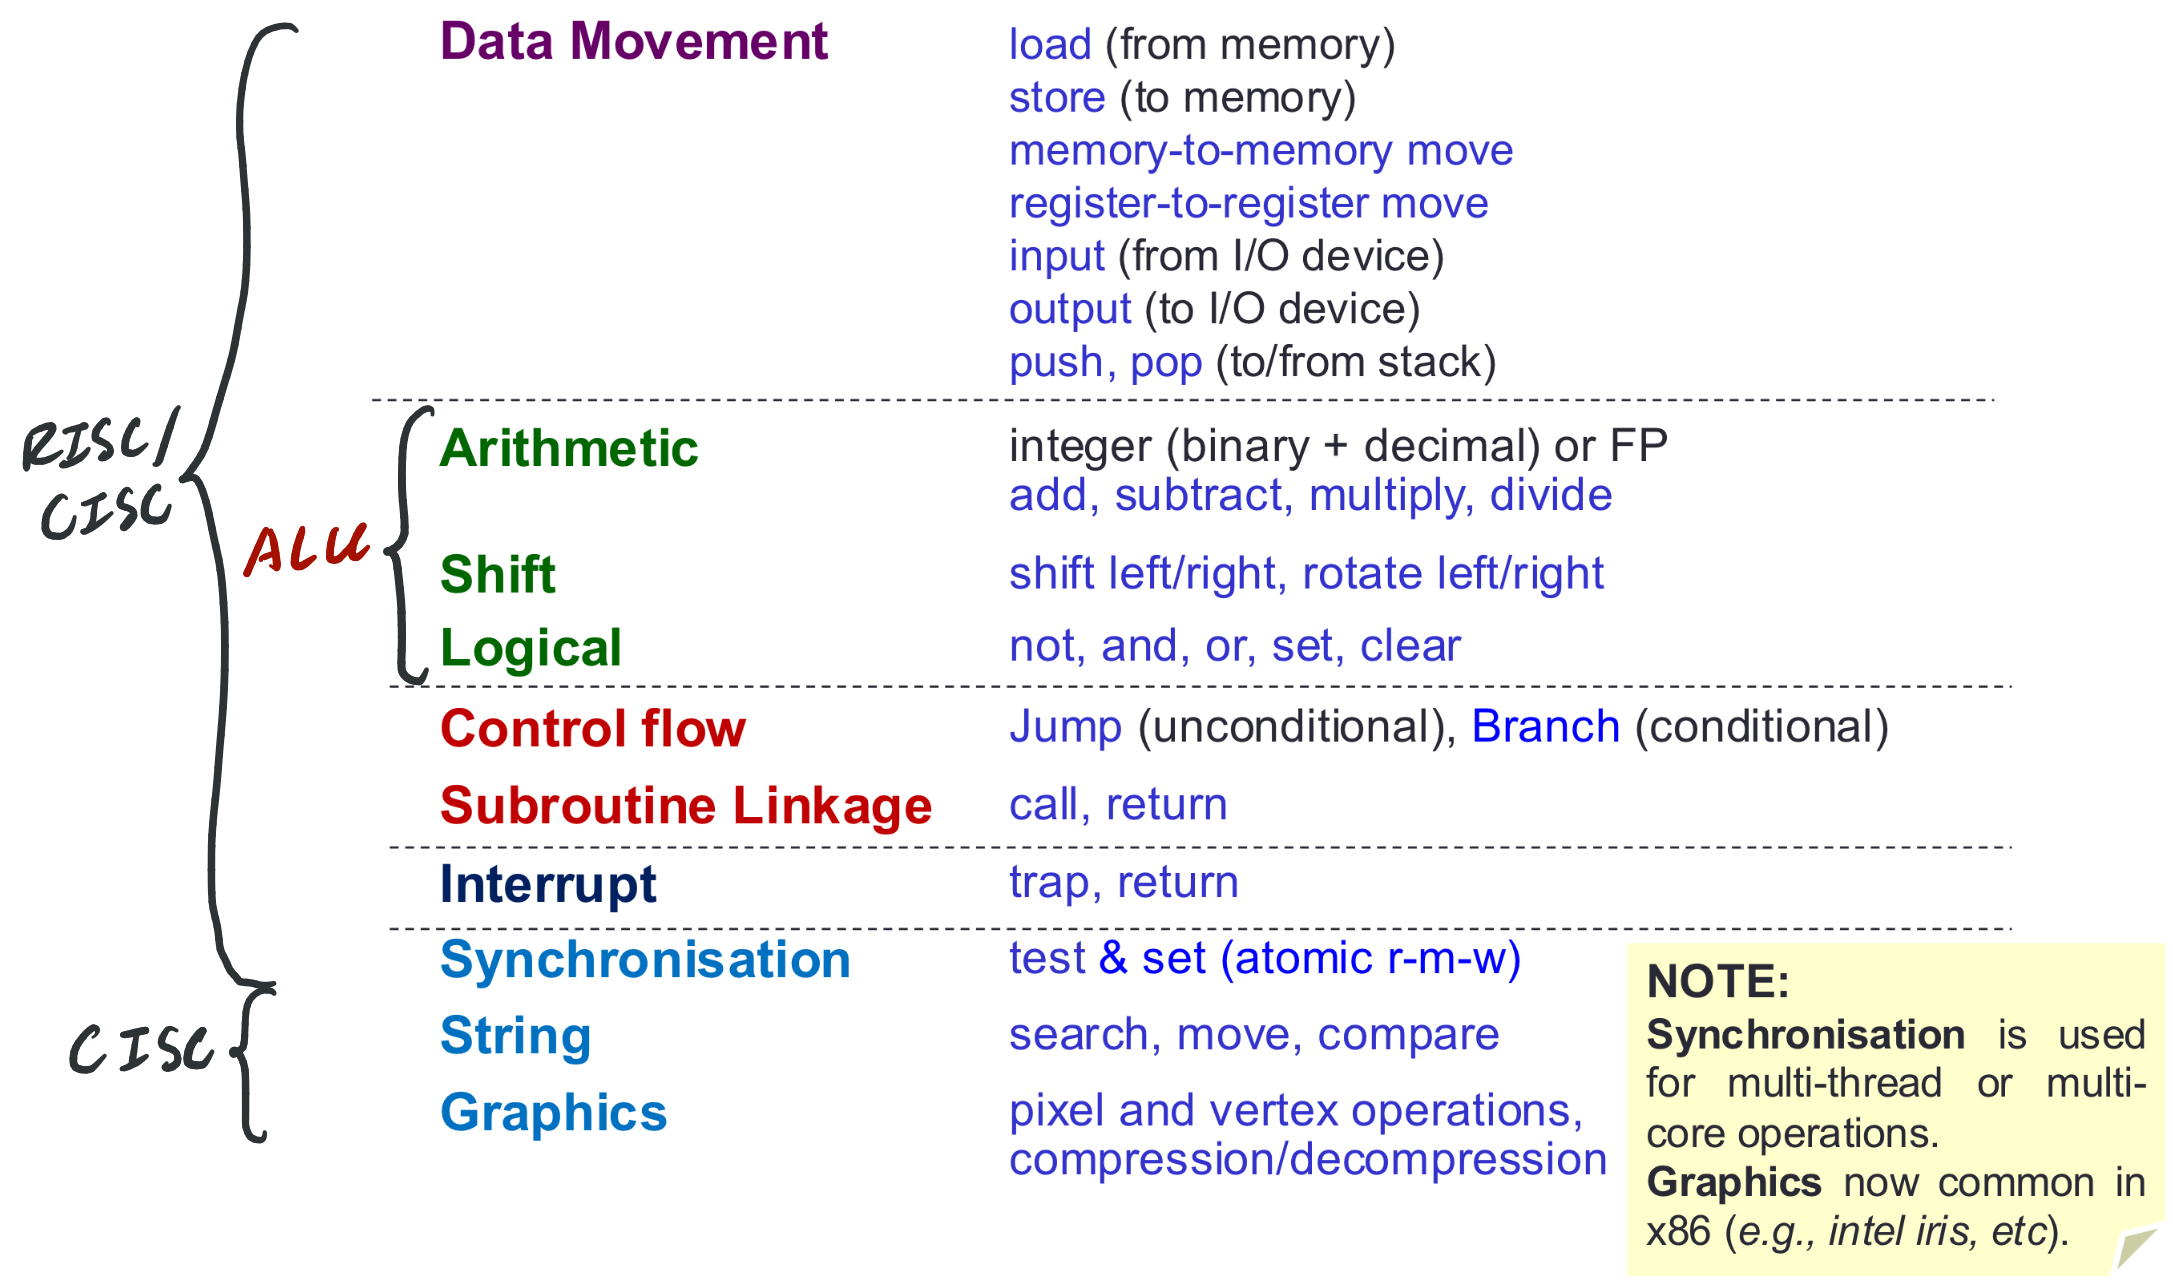
\includegraphics[width=0.75\textwidth]{instructionSet.jpeg}
\end{figure}

\subsubsection{Instruction Format}
An instruction consists of the \textit{opcode} (a unique code specifying the
operation) and the \textit{operands} (any additional information needed for the
operations). The operation \textbf{designates} the type and size of the
operands.
\begin{multicols}{2}
  \textbf{Variable-length} instructions: Used in most CISC.
  \begin{itemize}
    \item Requires multi-step fetch and decode
    \item Allows for more flexible and compact instruction set
  \end{itemize}
  \textbf{Hybrid} instructions: a mix of both.\\
  \textbf{Fixed-length} instructions: Used in most RISC
  \begin{itemize}
    \item Allows for easy fetch and decode
    \item Simplifies pipelining and parallelism
    \item Instruction bits are scarce
  \end{itemize}
\end{multicols}

\subsubsection{Encoding the Instruction Set}
\begin{figure}[h!]
  \centering
  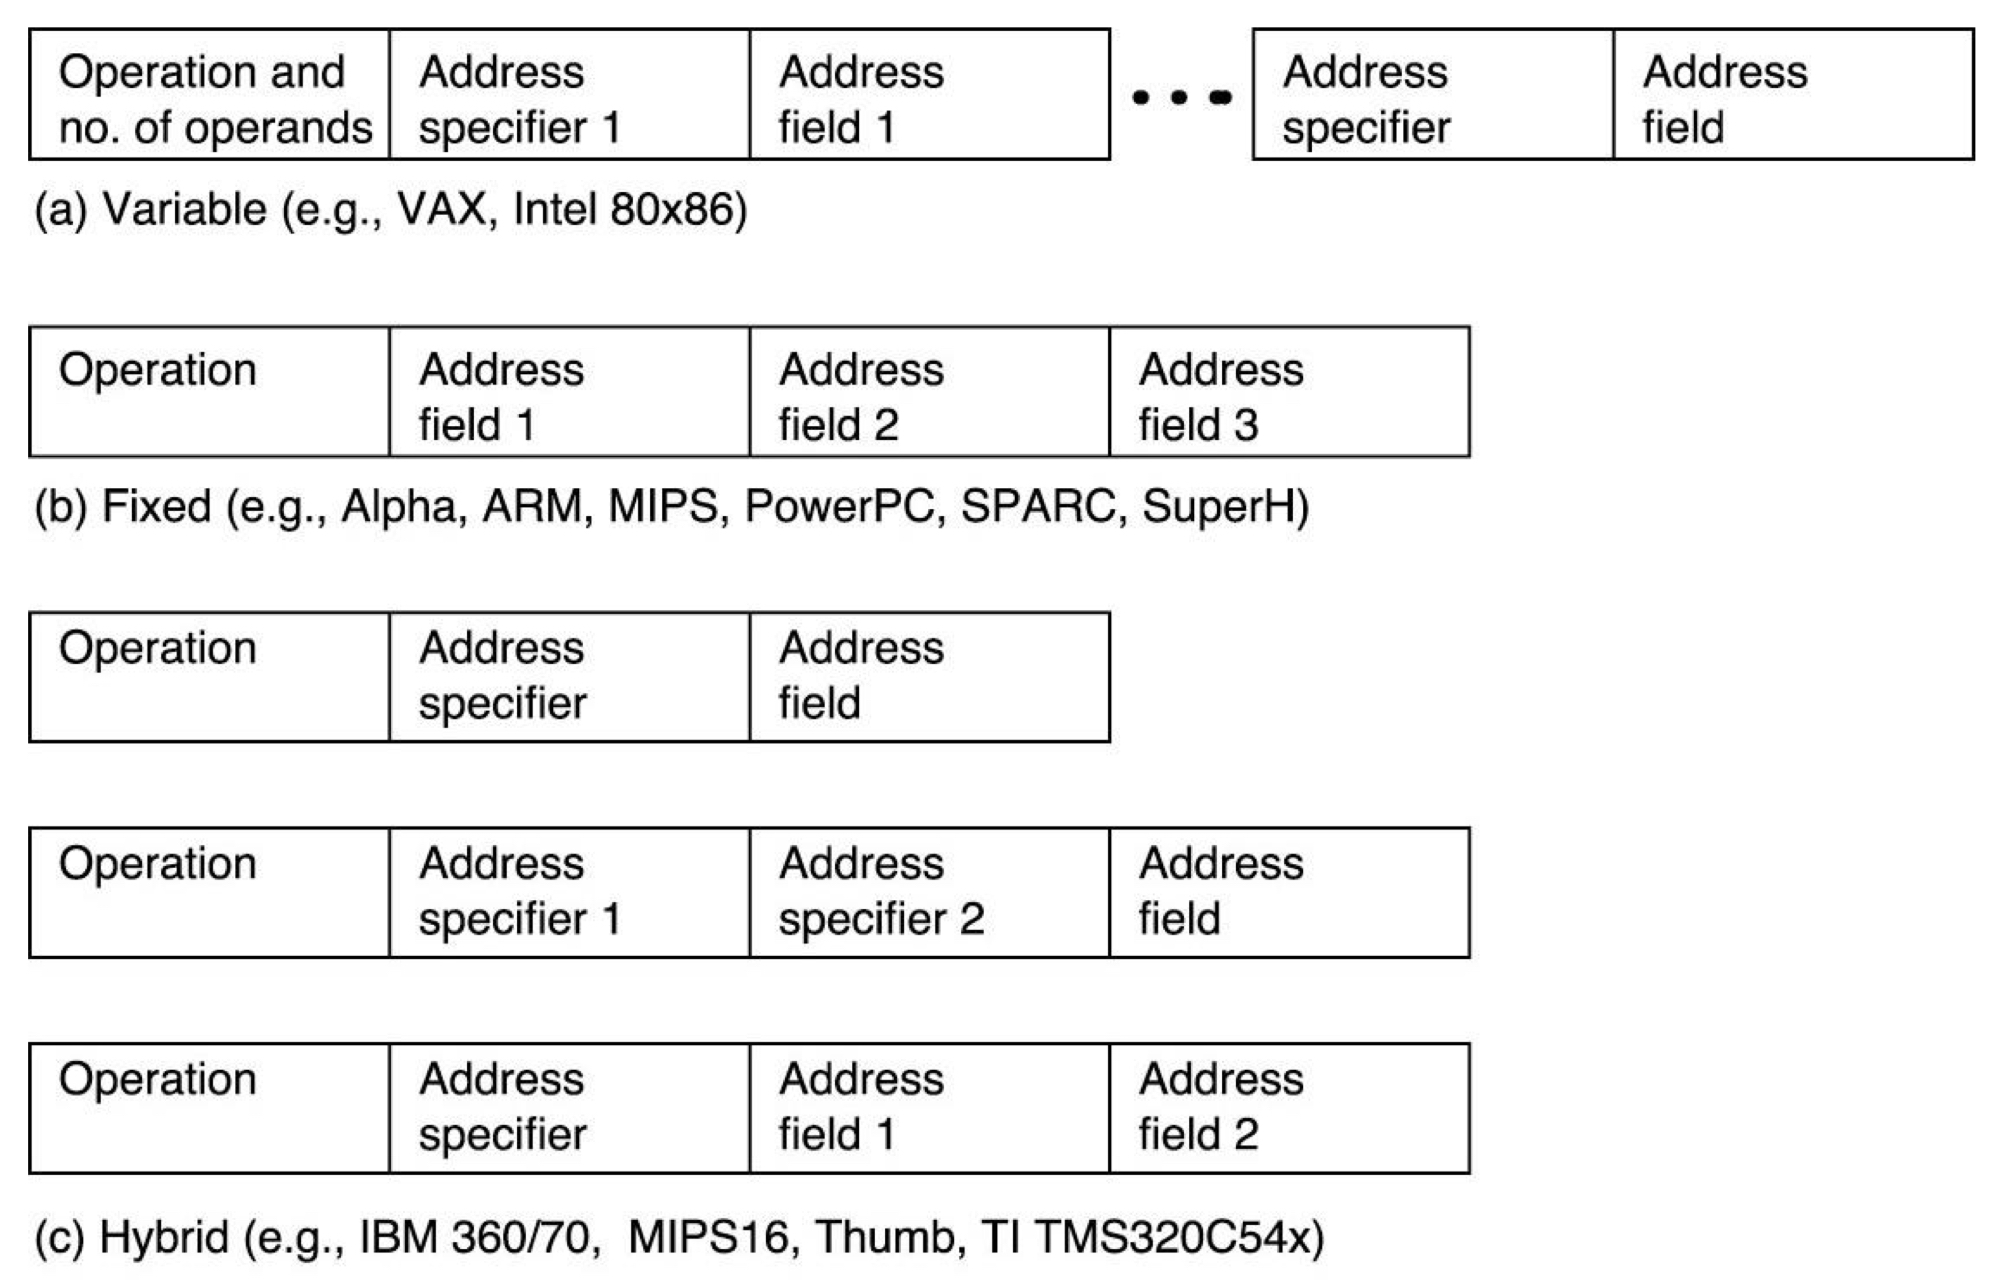
\includegraphics[width=0.6\textwidth]{encoding.jpeg}
\end{figure}
With fixed length instructions, we may adopt an \textbf{expanding opcode}
scheme. That is, the opcode has different lengths for different instructions.
\begin{example}[Maximum/Minimum Number of instructions]
  Given a $16$-bit instruction consisting type-A instructions with 6-bit
  opcodes and type-B instructions with 11-bit opcodes, the \textbf{maximum
  number of instructions} is given by maximising the prefixes for type-B,
  \[1 + \left( 2^{6}-1 \right) \times 2^{5} = 2017.\] 
  The \textbf{minimum number of instructions} is given by minimising the prefixes
  for type-B,
  \[1\times 2^{5}+2^{6}-1.\] 
  \begin{figure}[h!]
    \centering
    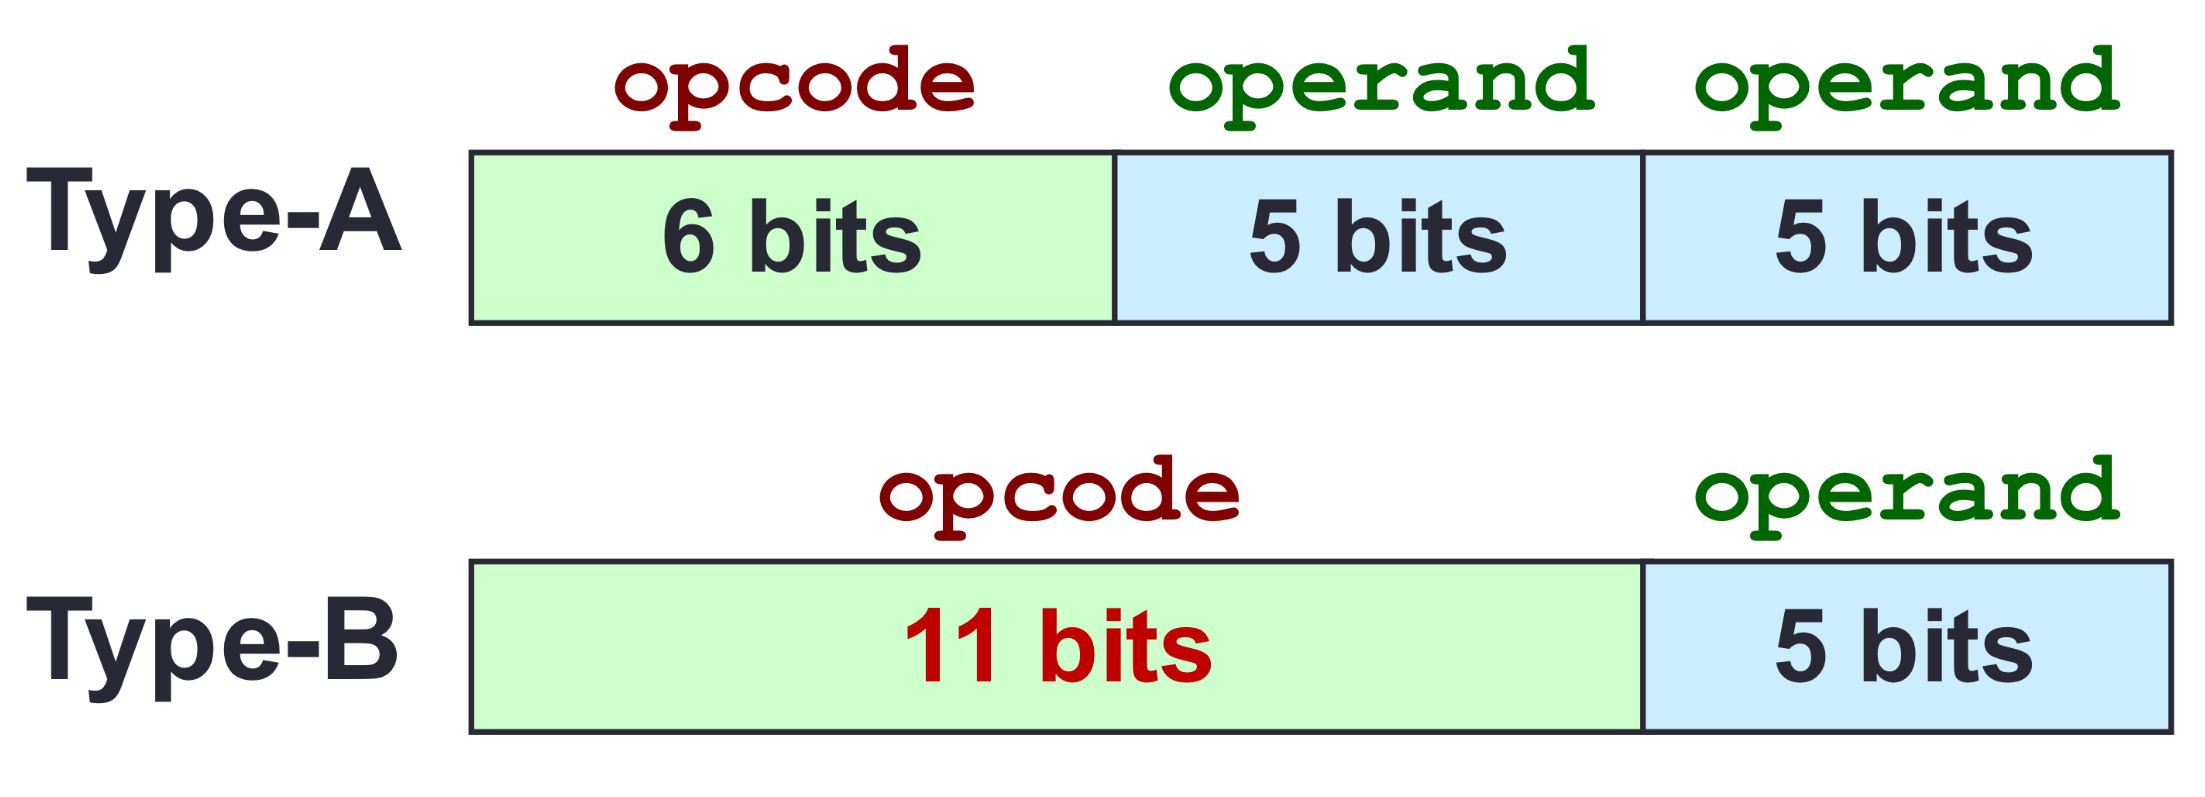
\includegraphics[width=0.35\textwidth]{expandingOpcode.jpeg}
  \end{figure}
\end{example}
To \textbf{design an expanding opcode} with specifications for the number of
instructions of each type, we first accommodate for the most restrictive case
(that is, the instruction type with the most operands).


\subsection{MIPS}
Microprocessor without Interlocked Pipelined Stages (MIPS) is a family of
RISC ISA\@. In summary, it adopts the stored-memory concept with the load-store
model:
\begin{itemize}
  \item \textbf{Stored-Memory Concept}: Instructions and data are stored in memory
  \item \textbf{Load-Store Architecture}: Faster processing by \textit{limiting
    memory access} through the bus, relying on registers for storage during
    execution
  \item The major \textbf{types of assembly instruction}: \textit{Memory},
    \textit{Calculation}, \textit{Control Flow}
  \item A typically assembly code structure is hence: (1) \textit{Load},
    (2) \textit{Compute}, (3) \textit{Store}
\end{itemize}
We typically have a limited number of registers in the processor. In MIPS, we
have $32$ registers, each referred to by its number or name. Registers
\textbf{do not have data types}, but each instruction assumes the data in the
register is of a certain type.
\begin{remark}
  In CS2100, we assume that we have enough registers to store all variables in
  our program.
\end{remark}
\begin{figure}[h!]
  \centering
  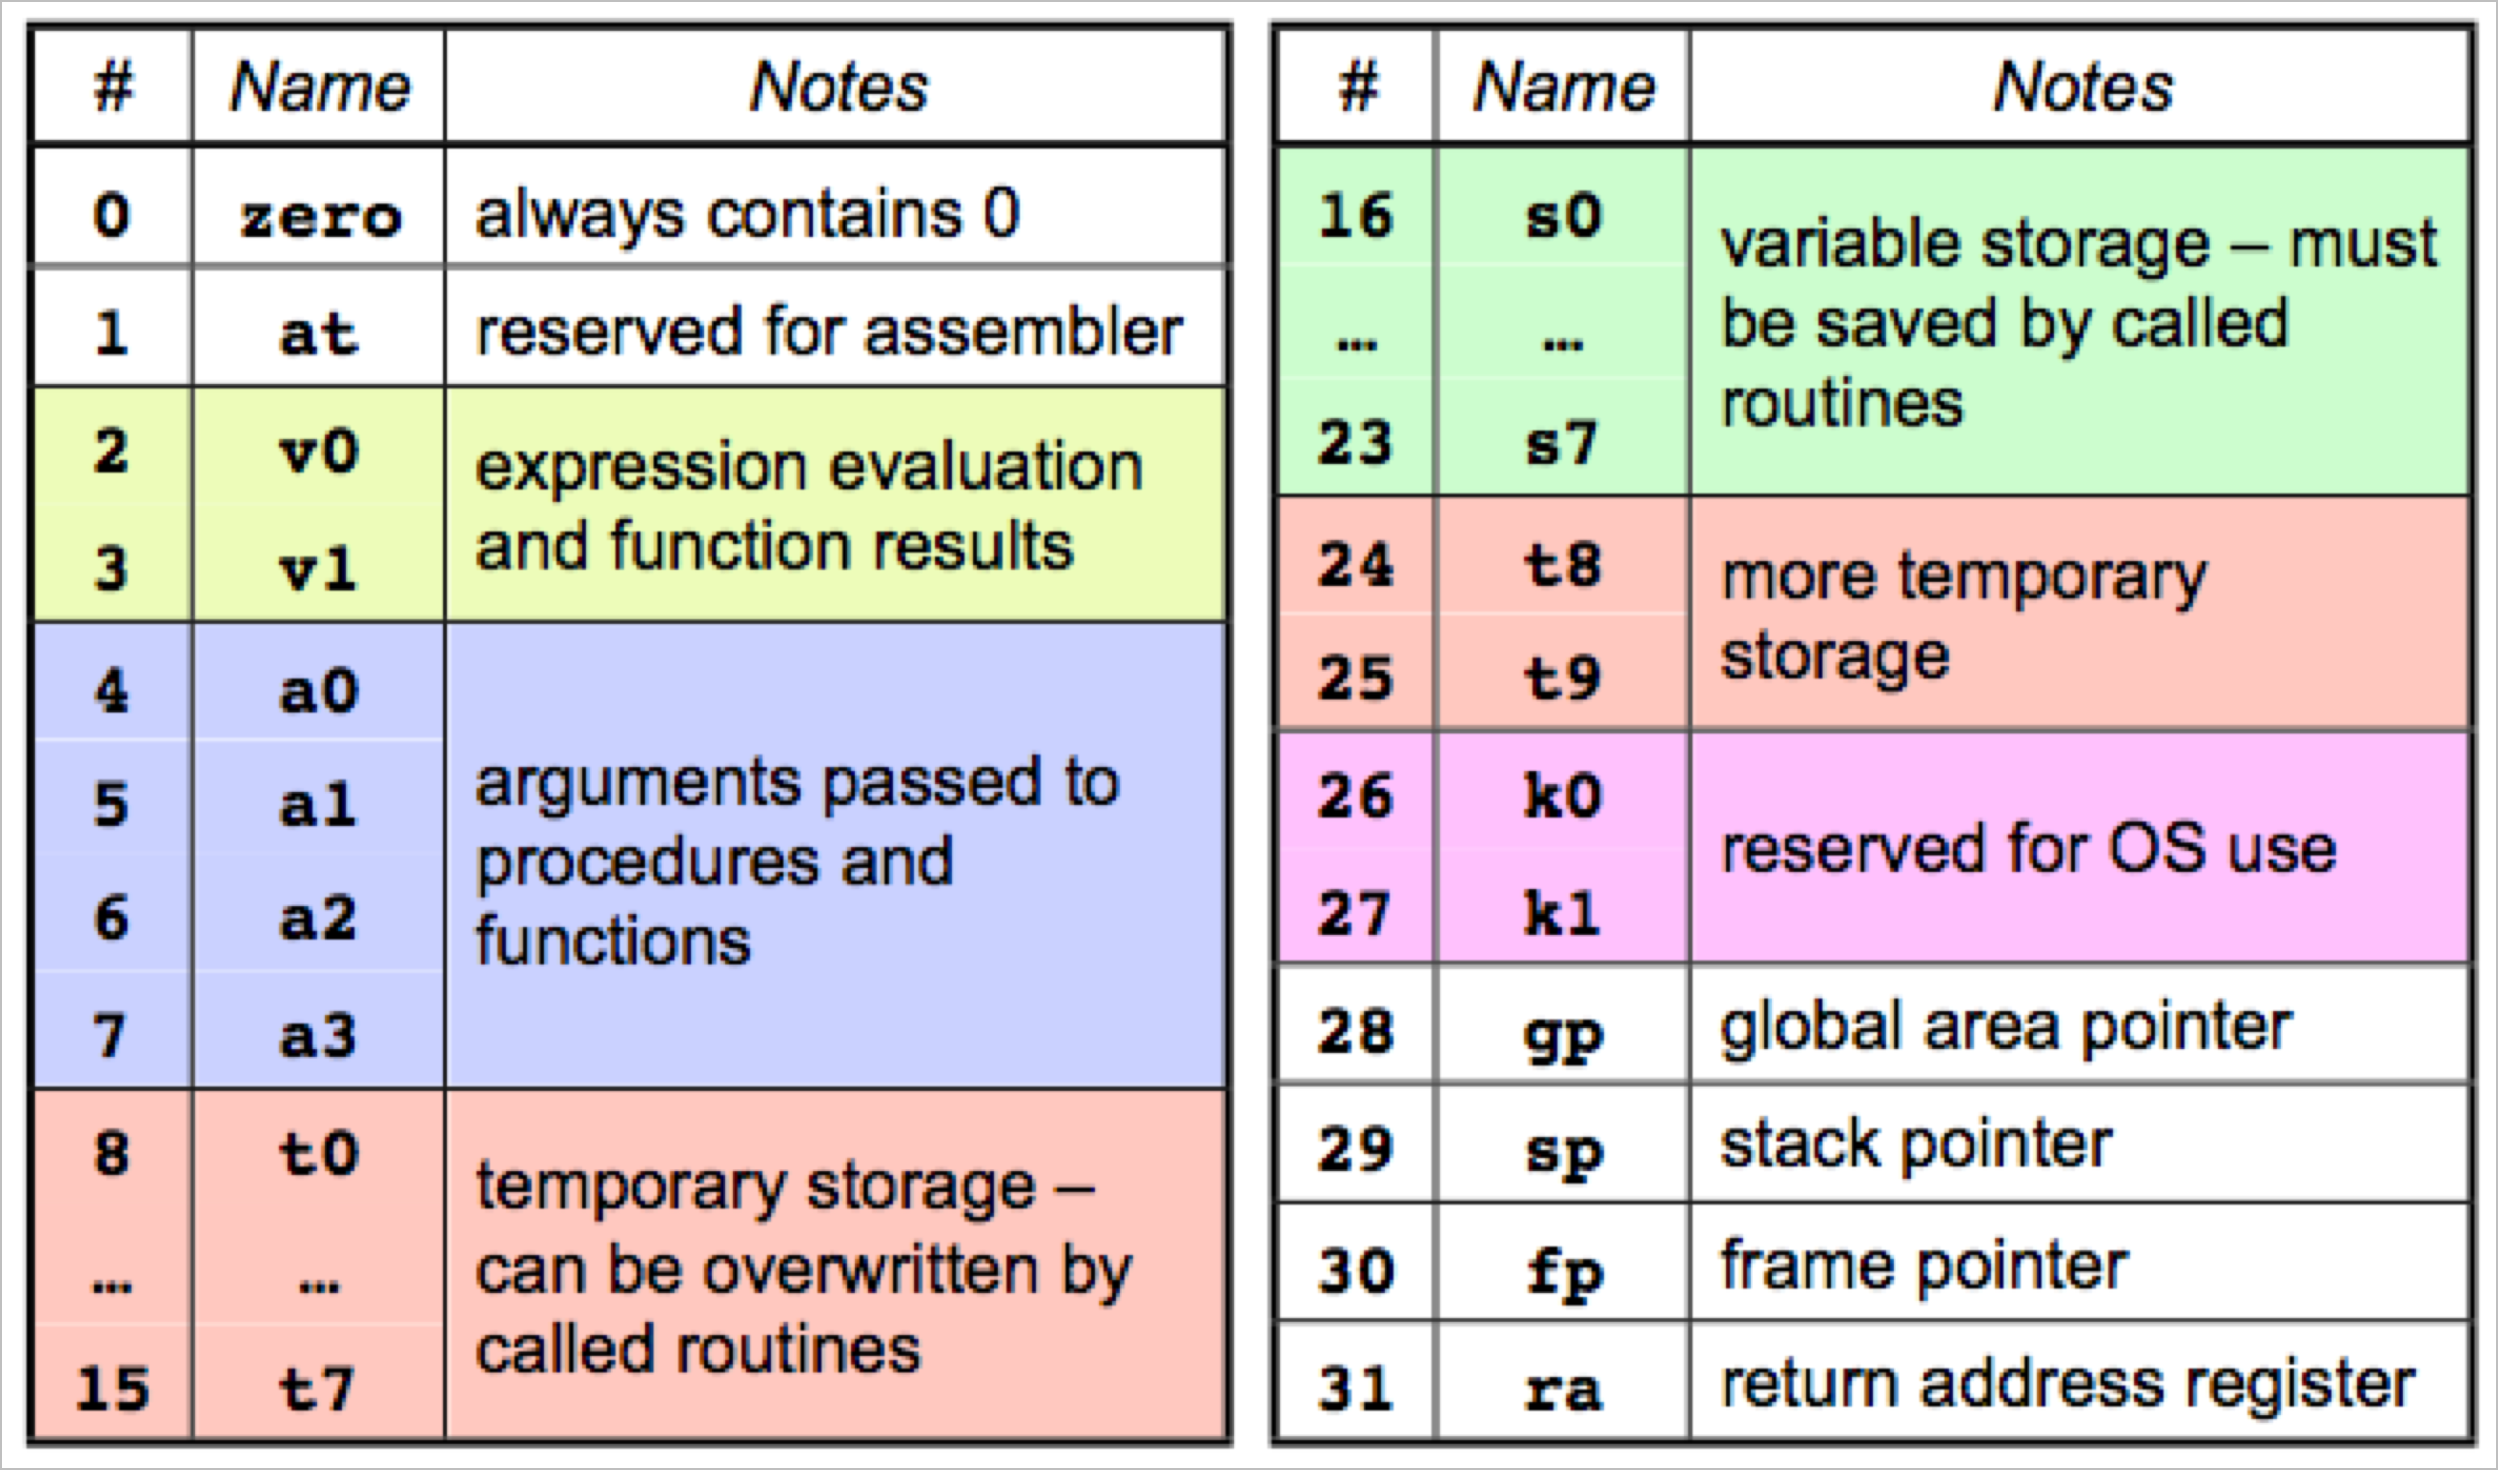
\includegraphics[width=0.65\textwidth]{registers.png}
\end{figure}

\subsubsection{MIPS Assembly Language}
\[\verb|op $r0, $r1, $r2|\qquad \verb|op $r0, $r1, Immd|\qquad \verb|op Immd|.\] 
Most MIPS (\textit{R-format}) operations consist three registers (1
destination, 2 sources).\ \textit{I-format} operations consist two registers (1
destination, 1 source) and an immediate value. While \textit{J-format}
operations uses only 1 immedate value.
\paragraph{Arithmetic Operations}
For arithmetic operations, The immediate ranges from $-2^{15}$ to $2^{15}-1$
(with a 16-bit 2s complement number system).
\paragraph{Logical Operations} In logical operations, the registers consist
of 32 raw bits, instead of a single 32-bit number.
\begin{figure}[h!]
  \centering
  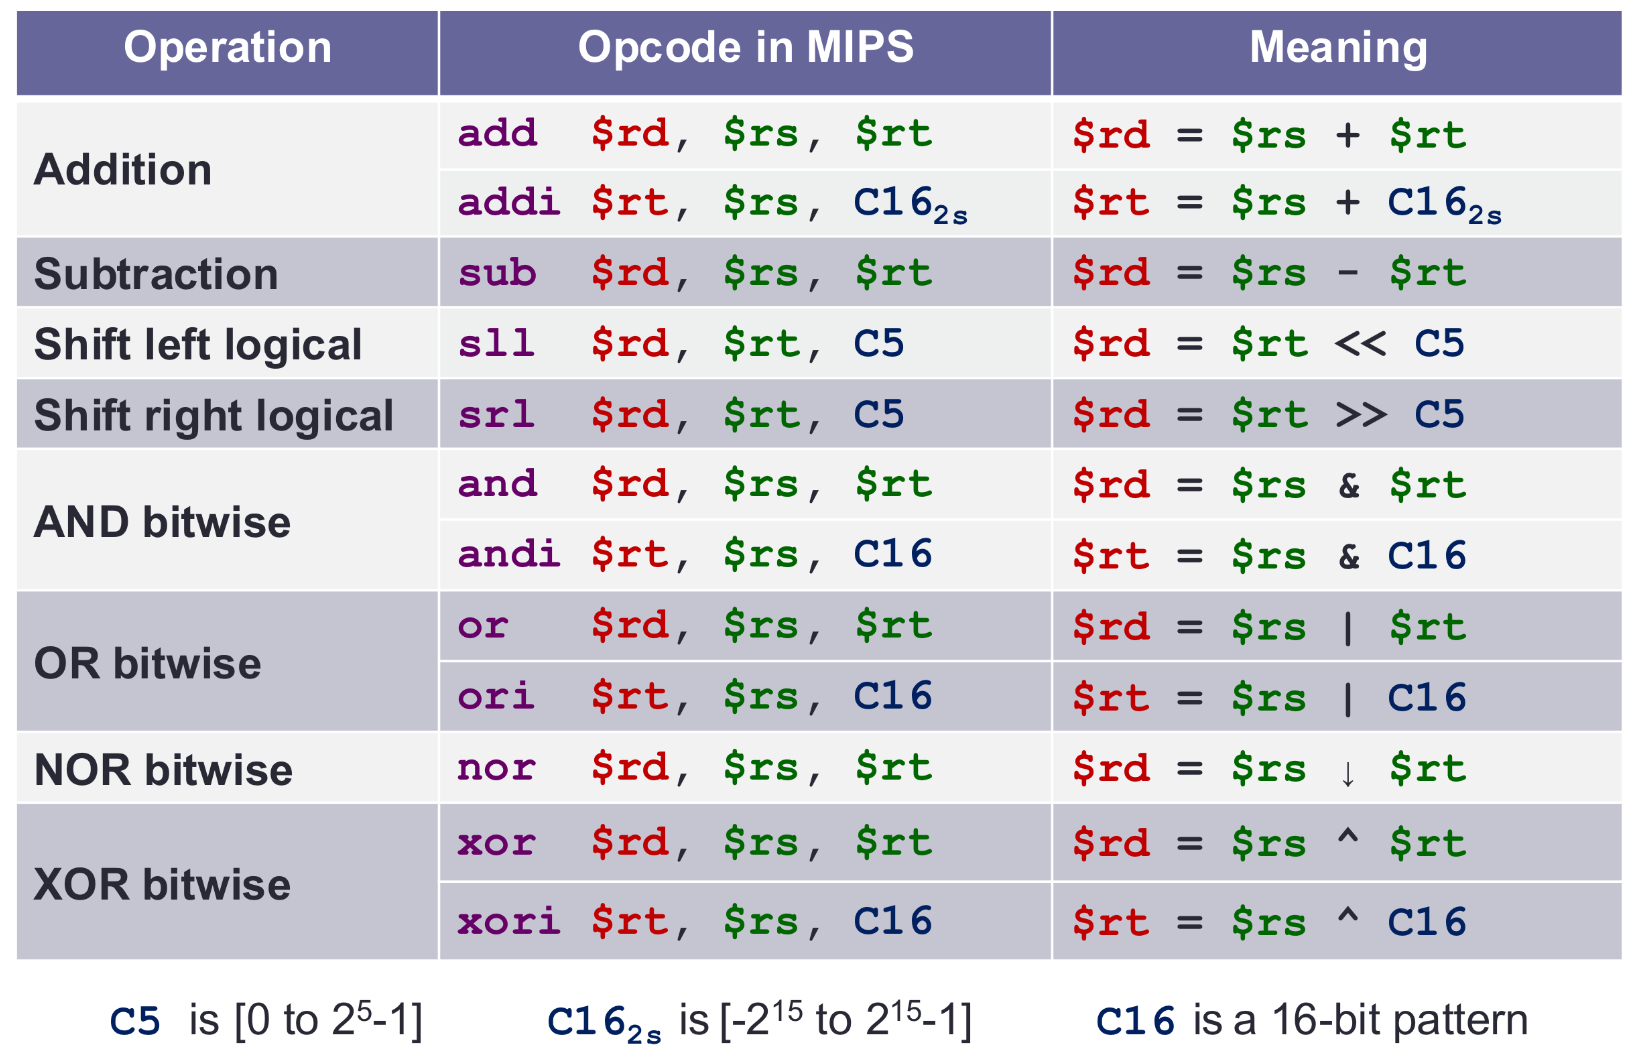
\includegraphics[width=0.6\textwidth]{mipsBasic.jpeg}
\end{figure}

\paragraph{Memory Organisation}
In MIPS, the main memory can be viewed as a \textit{large, single-dimensional
array} of memory locations. Each location has an address, sequentially indexed
in the array (in bytes). This is known as \textit{byte addressing}.

\begin{remark}
  With the byte address, we can access a single byte (\textit{byte
  addressable}) or a single word (\textit{word addressable})
\end{remark}

MIPS consists of $32$ registers, each $32$-bit (4-byte) long. Each word contains
32 bits (4 bytes) and memory addresses are $32$-bit long.\ \textbf{Each word is
aligned in memory, that is, it begins at a byte that is a multiple of $4$.}
Hence, we have the memory instructions \verb|lw $t0, 12($t1)|,
\verb|sw $t0, 12($t1)| requiring the address be a multiple of 4. To load/store
misaligned values, we use the instructions \verb|lb| and \verb|sb| instead.

\begin{definition}[Variable Mapping]
  In C, during compilation, the compiler allocates a register for each variable used
  in the program. This process is known as \textbf{variable mapping}.
\end{definition}

\begin{example}[Large Constant Loading]
  To load a large (>16 bits) immediate, we first set the upper 16-bit:
  $\verb|lui $t0, 0xAAAA|$, then set the lower 16-bits:
  $\verb|ori $t0, $t0, 0xAAAA|$
\end{example}

\paragraph{Control Flow}
In performing general computing tasks, we are required to make decisions
(conditions) and perform iterations (loops). To alter the control flow of the program,
we have:
\begin{itemize}
  \item \textbf{Conditional} (branch) instructions
    \[\verb|bne $t0, $t1, label|.\] 
    \[\verb|beq $t0, $t1, label|.\] 
  \item \textbf{Unconditional} (jump) instructions
    \[\verb|j label|\]
\end{itemize}
\begin{remark}
  Labels are ``anchors'' in the assembly code indicating branch targets. They
  are not instructions nor variables, and \textbf{no memory is allocated}.
\end{remark}
These instructions (along with \verb|slt| and \verb|slti|) allow us to
implement any loop or conditional decision making in our programs.
\begin{example}[Array Loops]
  For instance, we may implement array loops as follows:
  \begin{figure}[h!]
    \centering
    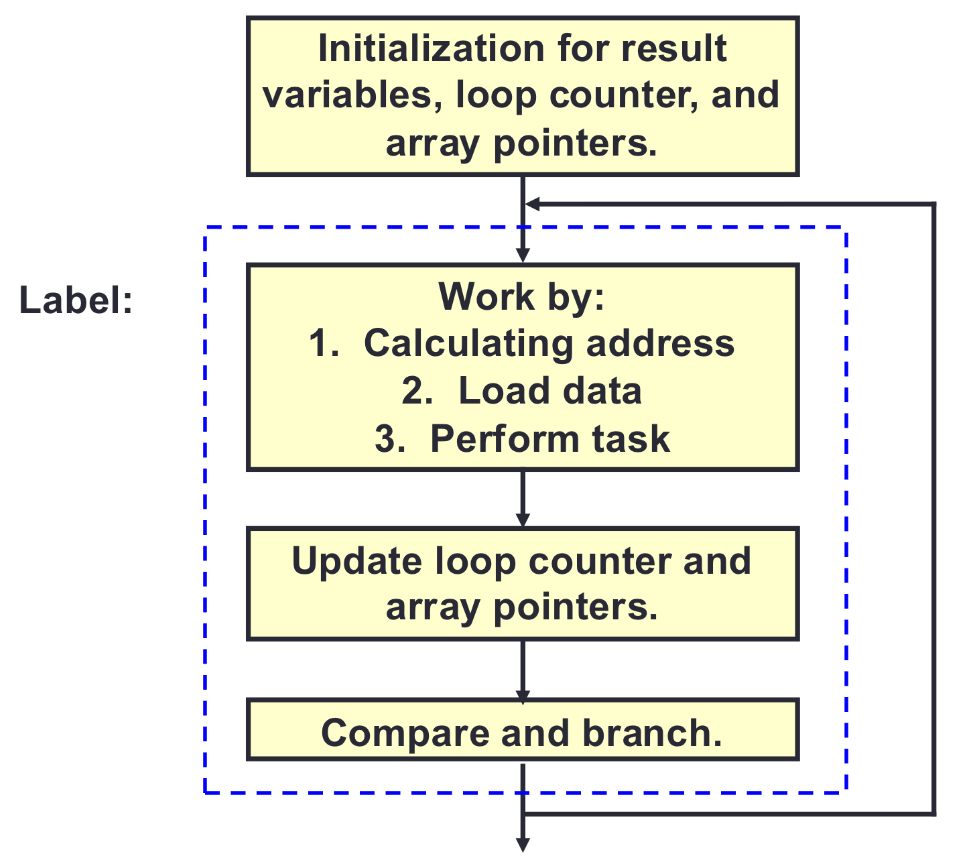
\includegraphics[width=0.4\textwidth]{controlFlow.jpeg}
  \end{figure}\\
  Another optimisation would be to directly use a array pointer instead of an
  index in many cases.
\end{example}

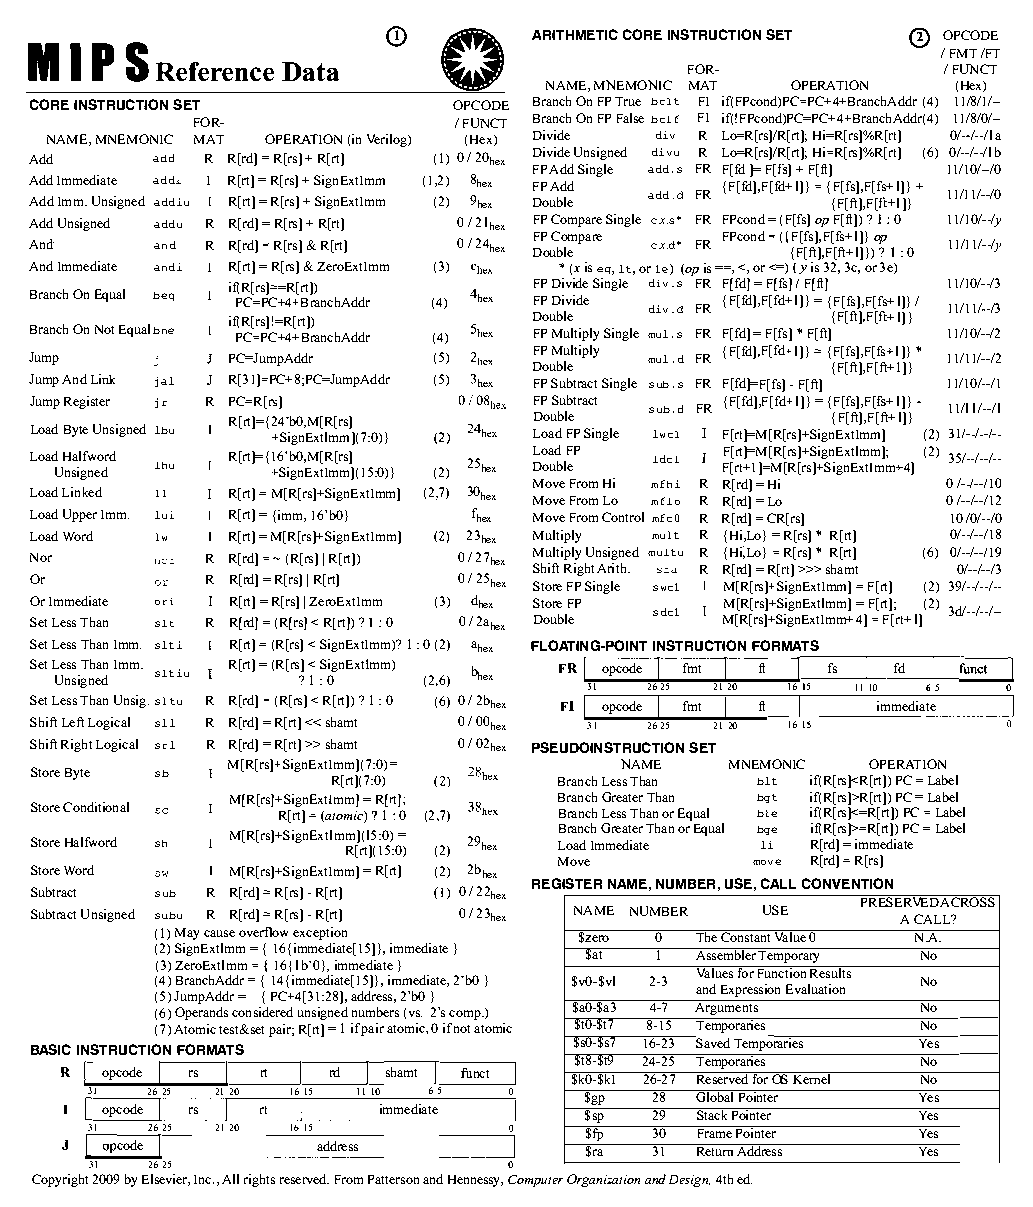
\includepdf[pages=-]{MIPS_Reference.pdf}

\subsubsection{MIPS Encoding}
Instructions in MIPS are classified into \textit{Register Format},
\textit{Immediate Format}, or \textit{Jump format}, according to their
operands. \textbf{Instructions with same operand types have the same encoding.}

\paragraph{R-Format} For register formats, we have the following fields:
\begin{itemize}
  \item \verb|opcode| Partially specifies the instruction, equals 0 $\forall$ R-format instructions
  \item \verb|funct| Further specifies the instruction
  \item \verb|rs| Source Register, specifies register containing the first operand 
  \item \verb|rt| Target Register, specifies register containing the second operand 
  \item \verb|rd| Destination Register, specifies register to receive the
    result of computation
  \item \verb|shamt| Shift Amount, equals 0 $\forall$ non-shift instructions
\end{itemize}
\begin{figure}[h!]
  \centering
  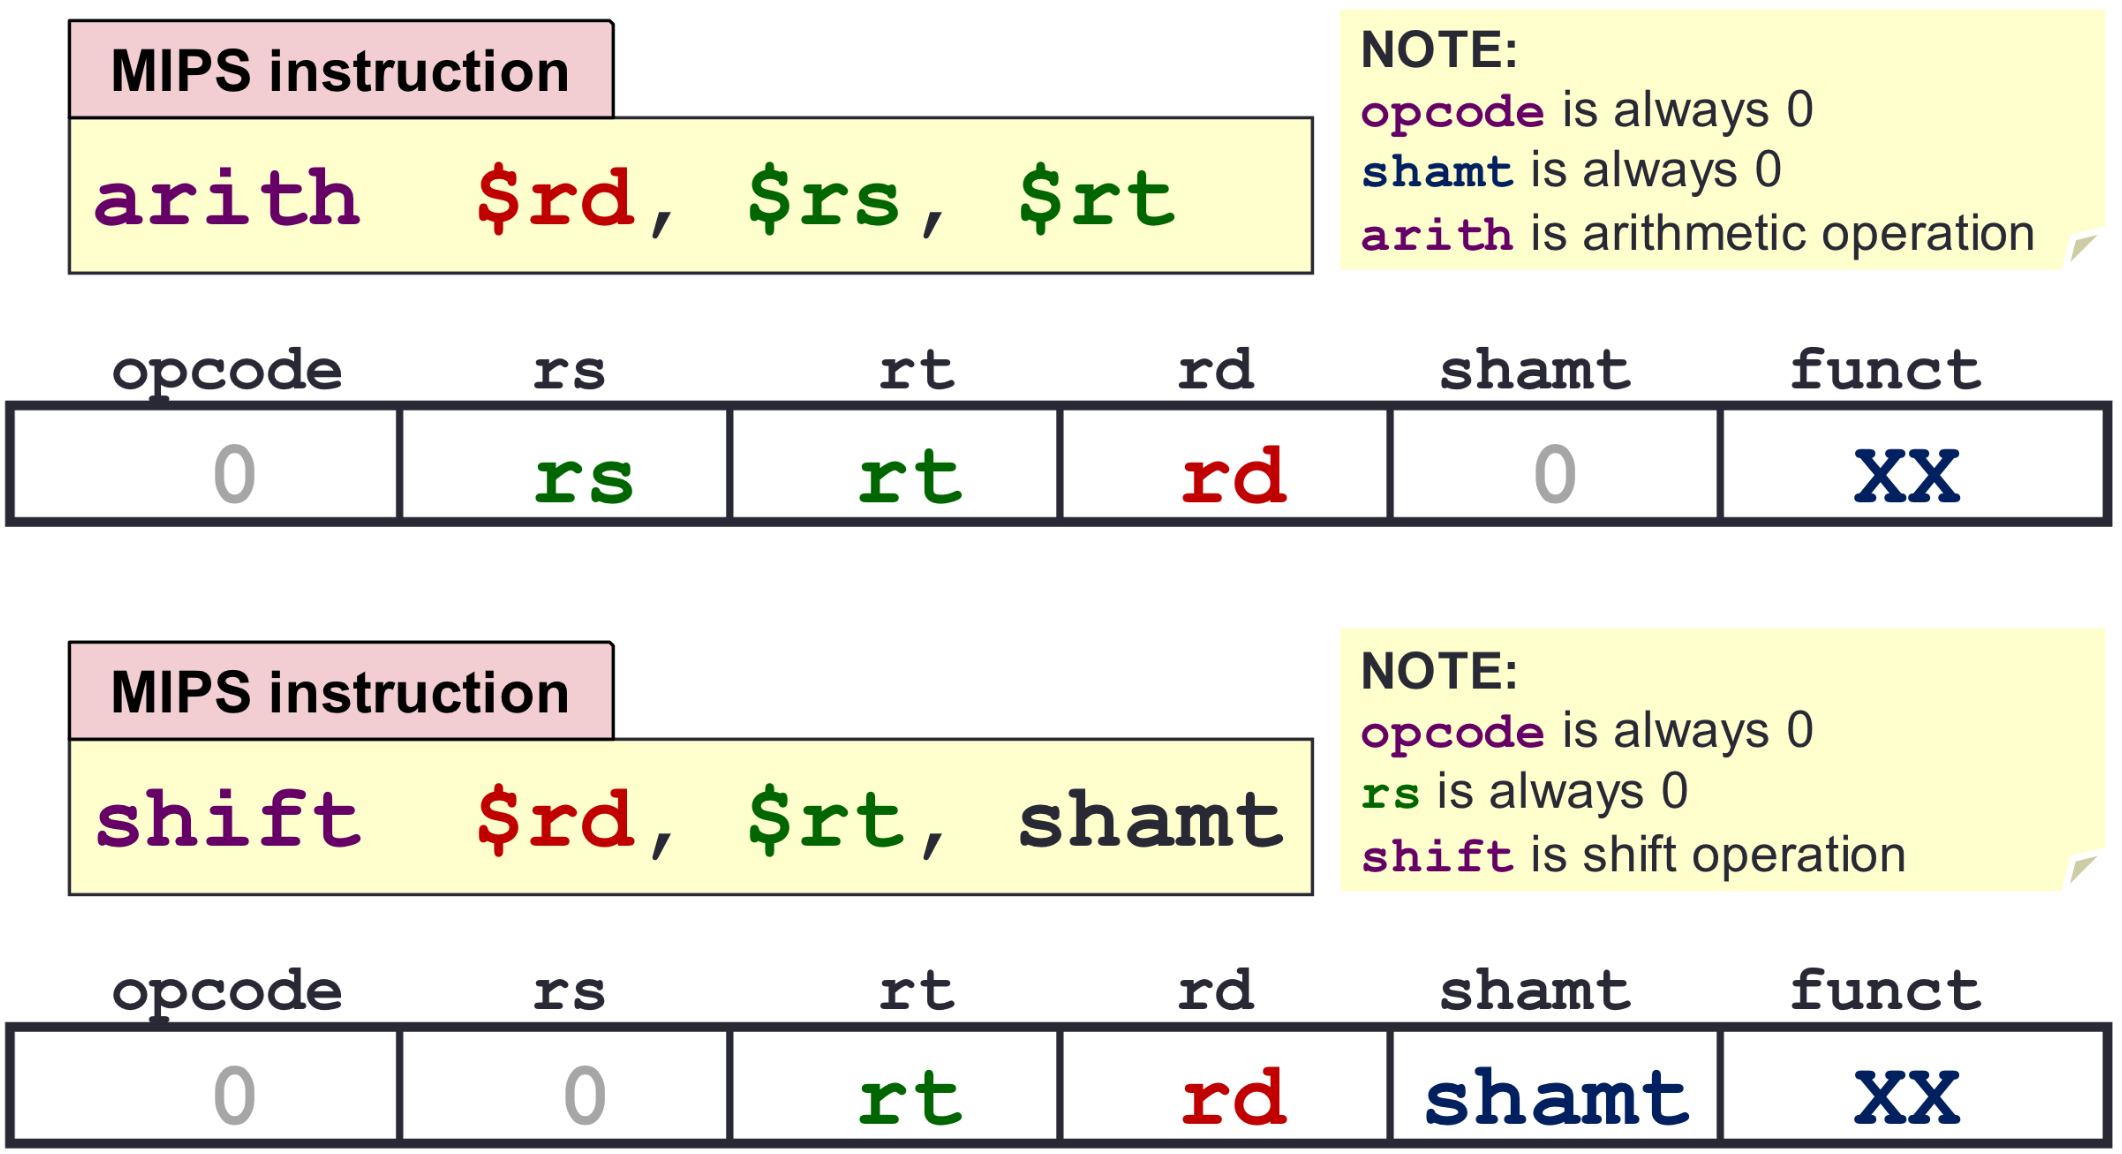
\includegraphics[width=0.4\textwidth]{rFormat.jpeg}
\end{figure}

\paragraph{I-Format} For immediate formats, we have the following fields:
\begin{itemize}
  \item \verb|op| Uniquely specifies the instruction
  \item \verb|rs| Specifies the source register operand (if any)
  \item \verb|rt| Specifies the target register to receive the result
  \item \verb|immediate| Taken as a signed integer in 2s complement
    (\textit{except for logical operations})
\end{itemize}
\begin{figure}
\centering
\begin{subfigure}{.5\textwidth}
  \centering
  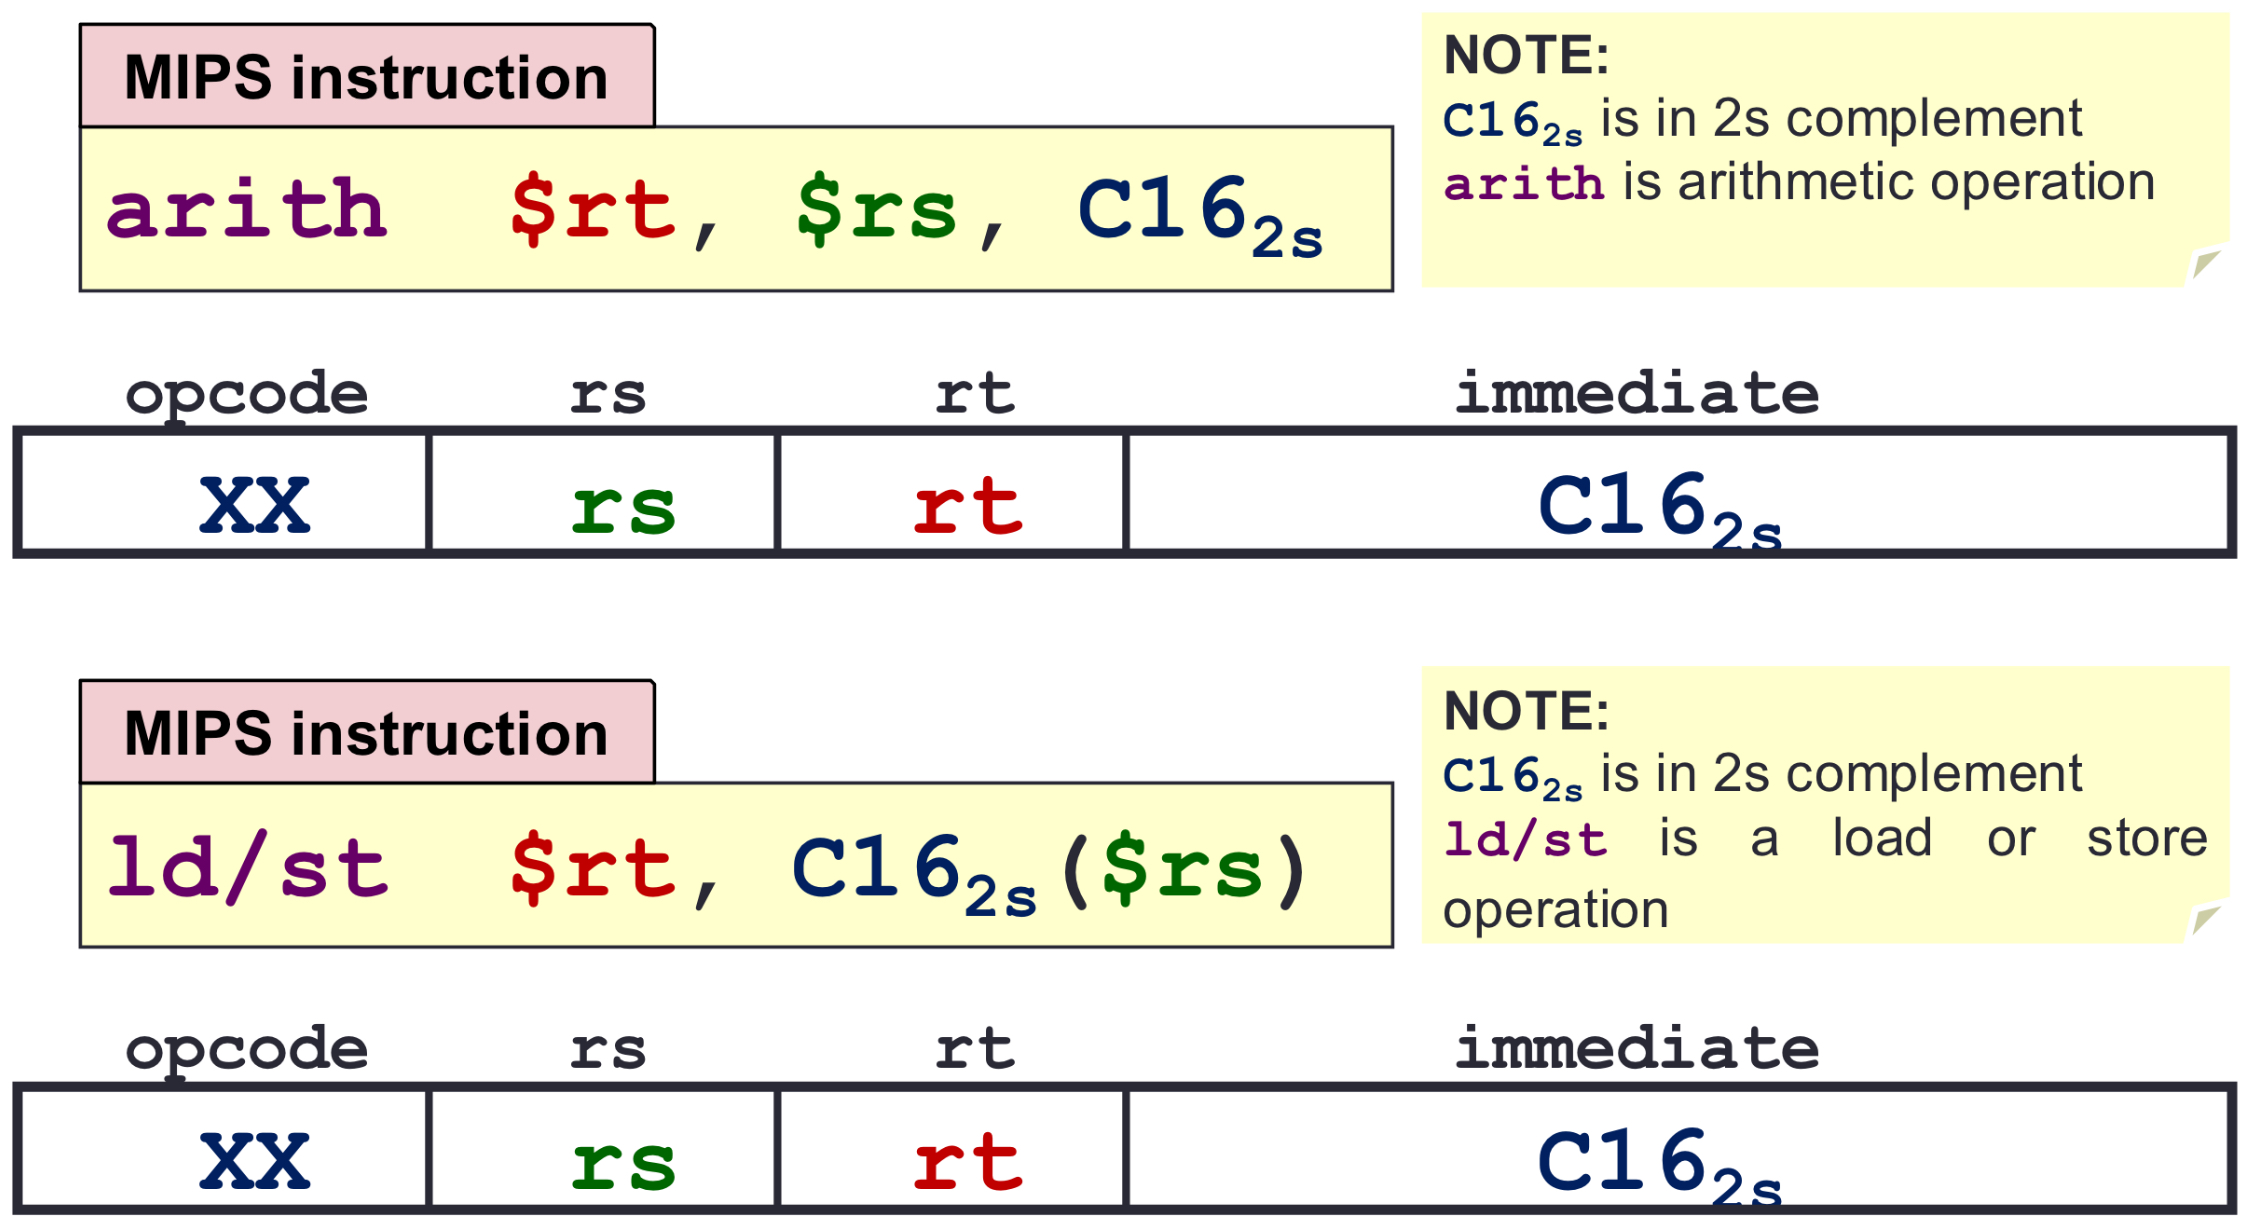
\includegraphics[width=.9\linewidth]{iFormat1.jpeg}
\end{subfigure}%
\begin{subfigure}{.5\textwidth}
  \centering
  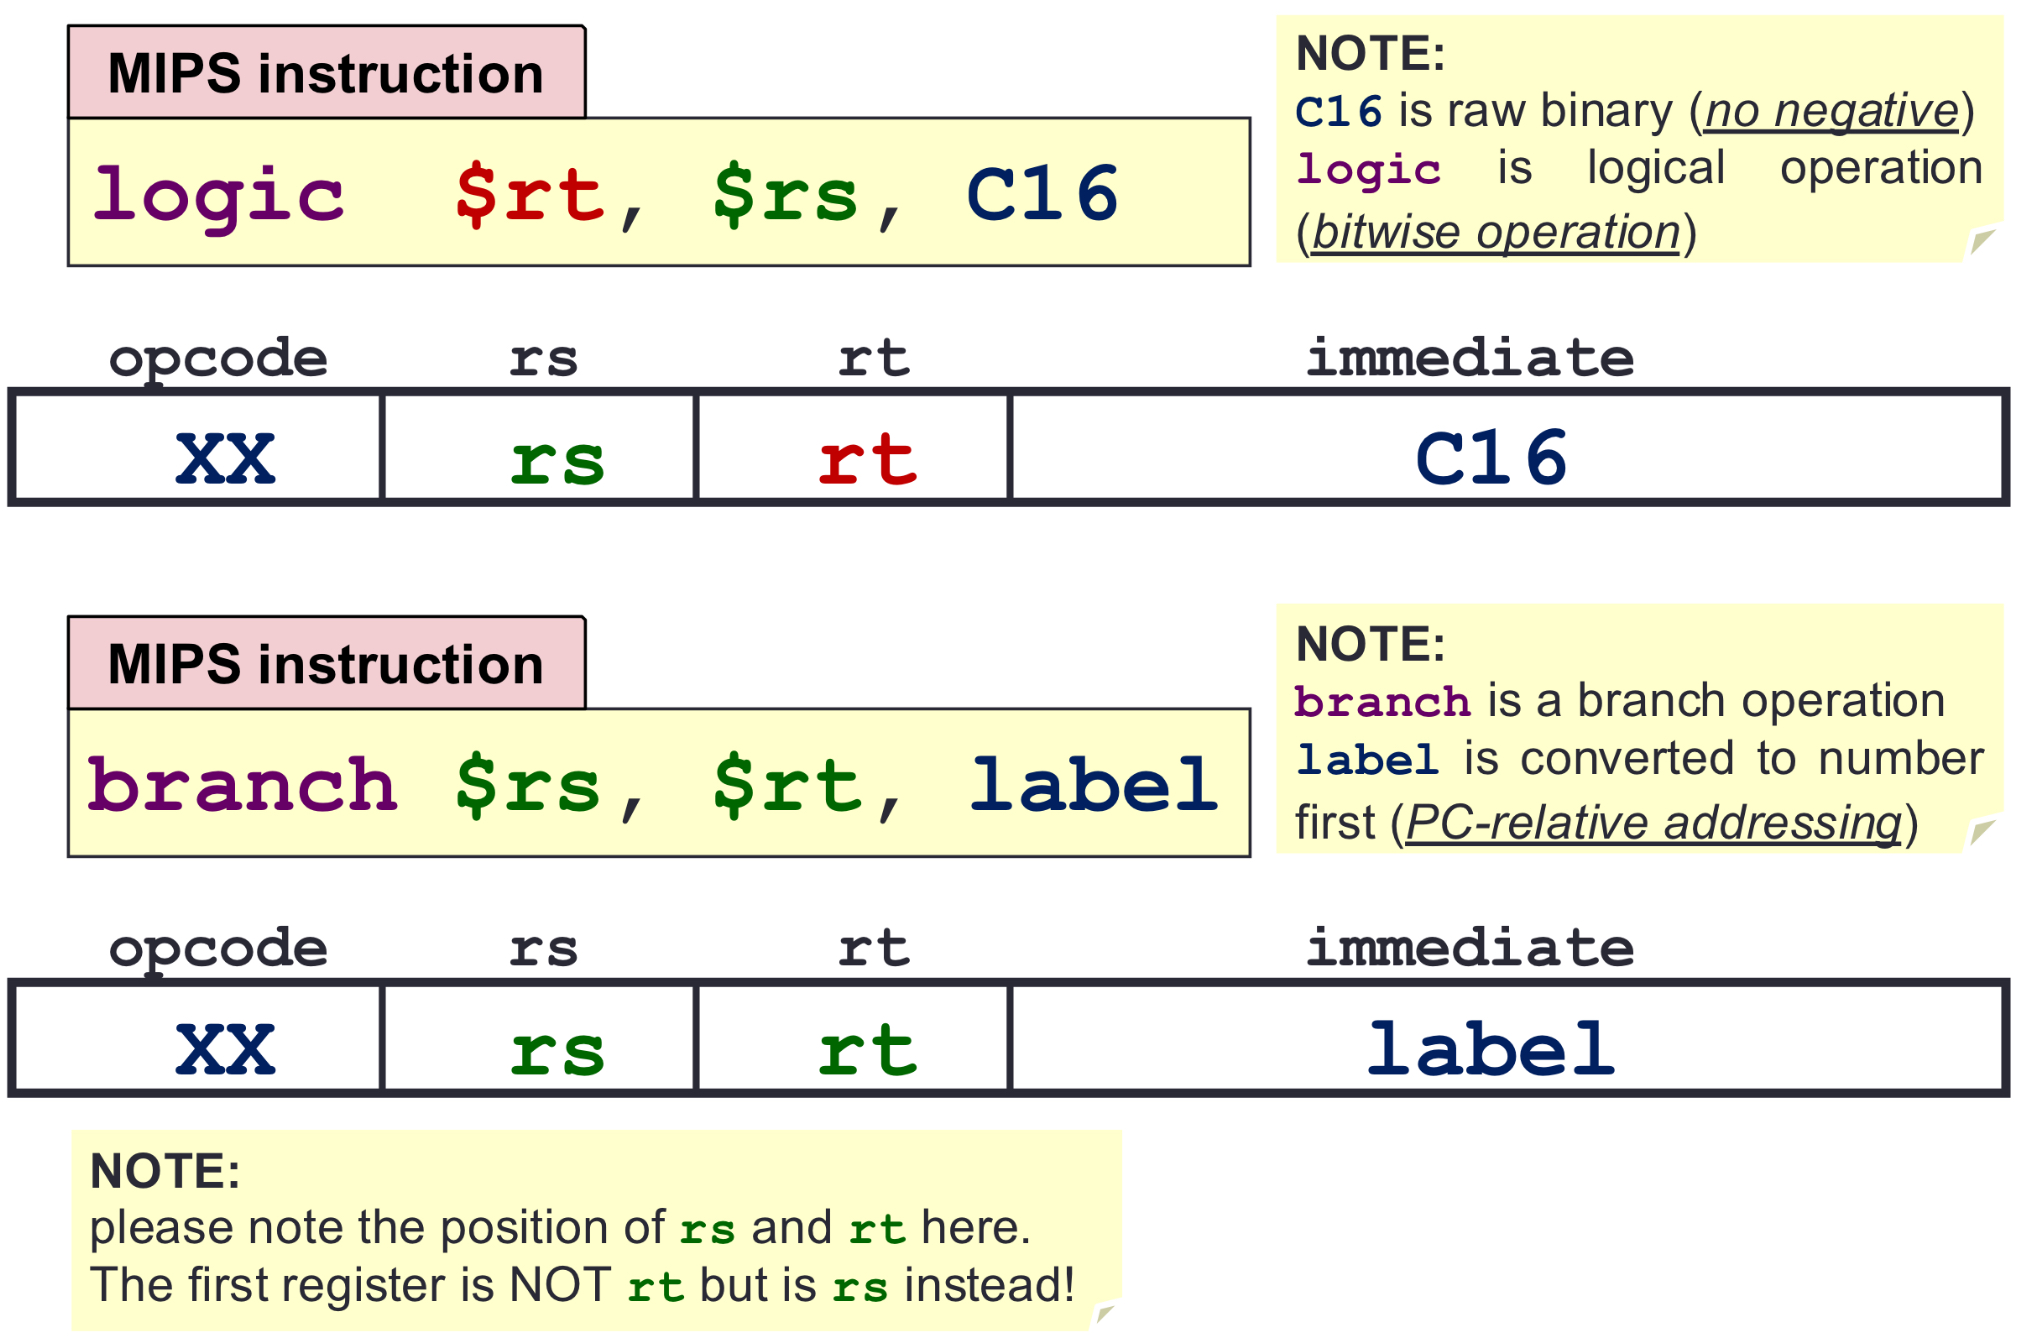
\includegraphics[width=.78\linewidth]{iFormat2.jpeg}
\end{subfigure}
\end{figure}
\begin{definition}[Program Counter]
  The \textbf{program counter} (PC) is a special register keeping address of
  the next instruction to be executed in the processor.
\end{definition}
Branch instructions also use the I-format, where the immediate specifies the
\textbf{relative address of the next instruction (in number of words)} if the
condition is fulfilled.
\[PC:=\begin{cases} PC+4&\text{if branch is not taken}\\ \left( PC+4 \right)
+\left( \verb|immediate| \times 4 \right) & \text{if branch is
taken}\end{cases}.\]
\begin{remark}
  This allows us to specify a branch up to $\pm 2^{15}$ words $=\pm 2^{17}$ 
  bytes from the PC.
\end{remark}

\paragraph{J-Format} For jump formats, we have the following fields:
\begin{itemize}
  \item \verb|opcode| Uniquely specifies the instruction
  \item \verb|targetAddress| Consists the 5th to 30th MSB of the target
    instruction address.
\end{itemize}
The 4 MSBs of the target instruction address is taken from $PC+4$, and the 2
LSBs are $00$ due to word alignment of instructions. We hence form the full
32-bit target address from the specified 26 bits.

\begin{remark}
  Due to the use of the first $4$-bits of $PC+4$, jump instructions are limited to within
  the same block of 256MB.
\end{remark}

\subsubsection{MIPS Addressing Modes}
In MIPS, we have the following addressing modes:
\begin{itemize}
  \item \textit{Register Addressing}: (\verb|add, sub, and, xor, nor, slt, sll, srl|)
  \item \textit{Immediate Addressing}: (\verb|addi, andi, ori, xori, slti|)
  \item \textit{Base Addressing (Displacement Addressing)}: Operand is at the
  address obtained from the sum of a register and an immediate (\verb|lw, sw|)
  \item \textit{PC-Relative Addressing}: Address is obtained from the sum of PC
  and an immediate (\verb|beq, bne|)
  \item \textit{Pseudo-direct Addressing}: Address is given by $26$-bit instruction
    concatenated with upper $4$-bits of $PC+4$
\end{itemize}

\section{Processor}
The processor comprises two major components: the \textbf{datapath} and the \textbf{control}.
\subsection{Datapath}
The datapath is the \textit{collection of components that process data}. It
performs the arithmetic, logical and memory operations.
\begin{remark}
  This processor design supports a subset of the core MIPS ISA:
  \begin{itemize}
    \item Arithmetic and Logical operations:
      \verb|add, sub, and, or, addi, slt, sll, srl|
    \item Data Transfer Instructions
      \verb|lw, sw|
    \item Branches
      \verb|beq, bne|
    \item Jumps
      \verb|j|
  \end{itemize}
  \verb|andi, ori| is not supported because sign extension is done on immediate
  values.
\end{remark}
\subsubsection{Instruction Execution Cycle}
The Instruction Execution Cycle comprises the following steps:
\begin{figure}[h!]
  \centering
  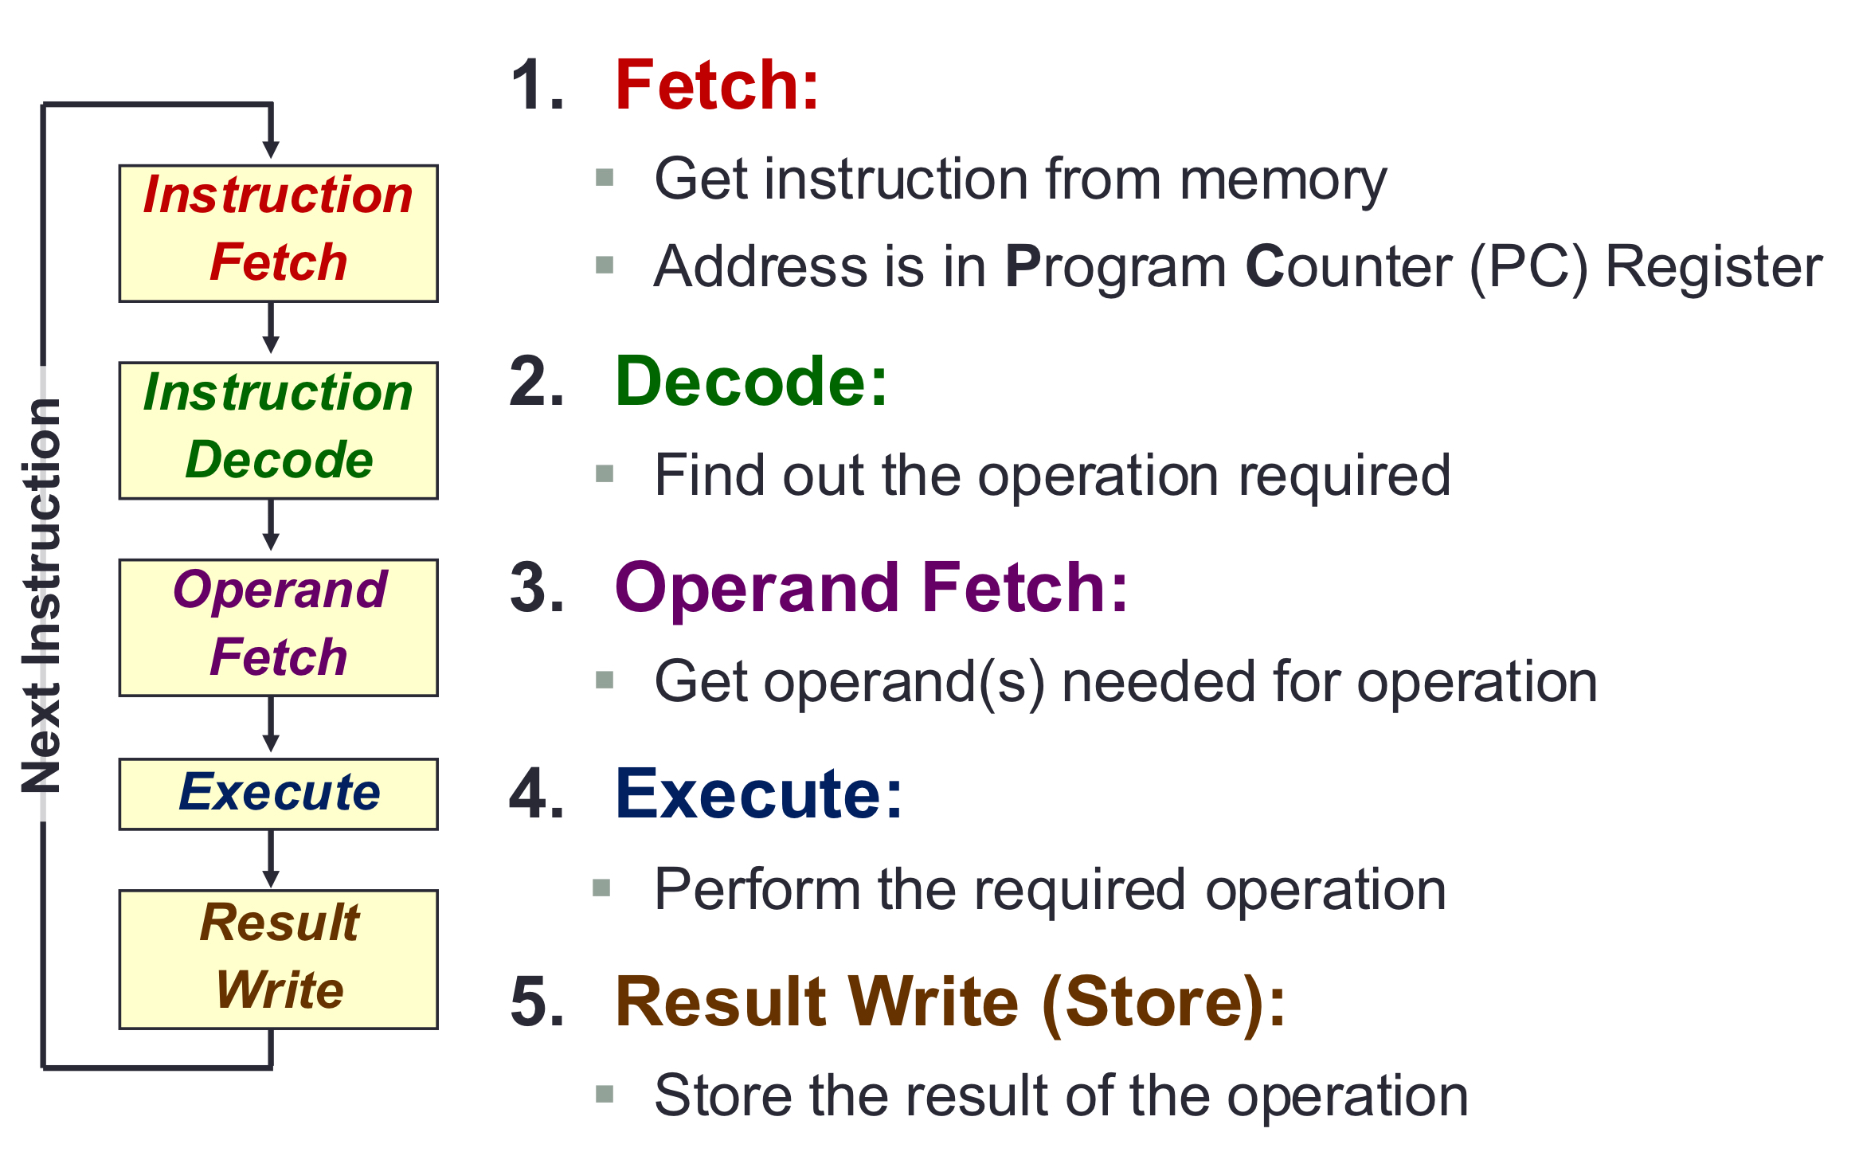
\includegraphics[width=0.5\textwidth]{IEC.jpeg}
\end{figure}
\paragraph{Instruction Fetch Stage}: Uses PC to fetch the instruction from
\textbf{instruction memory}, and then is incremented by $4$ to get the address of the next
instruction. Output instruction is then fed to the next stage.

\begin{definition}[Instruction Memory]
  The instruction memory is a sequential circuit that as an internal state
  storing the instructions. It also comprises a clock signal.
\end{definition}

\paragraph{Clock Period}
The clock signal ensures that we do not read and write the PC at the same time,
by ensuring that the PC is read during the first half of the clock period, and
updated at the \textbf{next rising clock edge}.\\
In general, the clock period allows us to read, compute, and write all within a
single clock period, and allow us to synchronise between each phase of the
instruction execution.


\paragraph{Instruction Decode/Operand Fetch Stage}: Gathers the data from the
instruction fields. It determines the instruction type and field lengths, and
then read from all necessary registers. The output operation and operands is
then fed to the next stage.

\begin{definition}[Register File]
  The register file is a collection of 32 registers that can be read/written by
  specifying the register number. Per instruction, a maximum of two registers
  can be read and one register can be written.
\end{definition}

\paragraph{Instruction ALU Stage}: Executes an operation specified by
ALUControl with the two input values. It outputs \verb|ALUresult| and
\verb|is0?|. The \verb|is0?| bit is used to generate the PCSrc Control signal
that decides whether there is a jump.

\begin{figure}[h!]
  \centering
  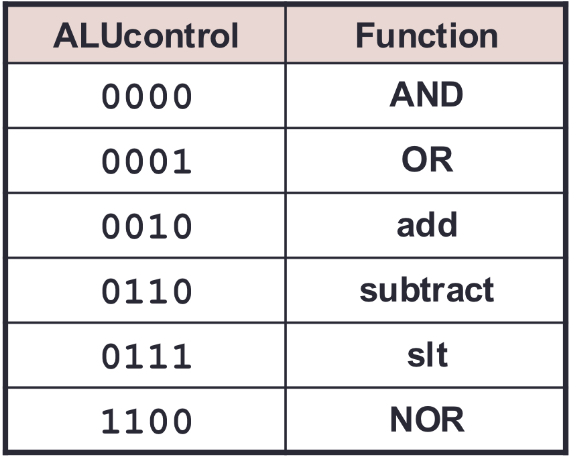
\includegraphics[width=0.25\textwidth]{aluControl.jpeg}
\end{figure}

\paragraph{Memory Stage}: For load and store instructions, we use the memory
address calculated by the ALU stage to read or write data memory. The output value
is passed on to the RegWrite stage.

\begin{definition}[Data Memory]
  The data memory is a storage element for the data of a program., taking in a
  memory address, data to be written and outputs the data read from memory for
  load instructions.
\end{definition}

\paragraph{RegWrite Stage}: For most instructions, we write the result of computation
into a register (except for stores, branches and jumps).

\subsection{Control}
The control prescribes the processes of the datapath, memory and I/O devices
according to program instructions, through control signals. From the datapath,
we are required to generate the control signals:

\begin{figure}[h!]
  \centering
  \includegraphics[width=0.7\textwidth]{controlSignals.jpeg}
\end{figure}

\paragraph{ALUControl Design}
Considering the 1-bit ALU, the ALUControl signal indicates whether to invert
each of the input, and specify the final operation performed on the inputs, as
shown in the figure.

\begin{figure}[h!]
  \centering
  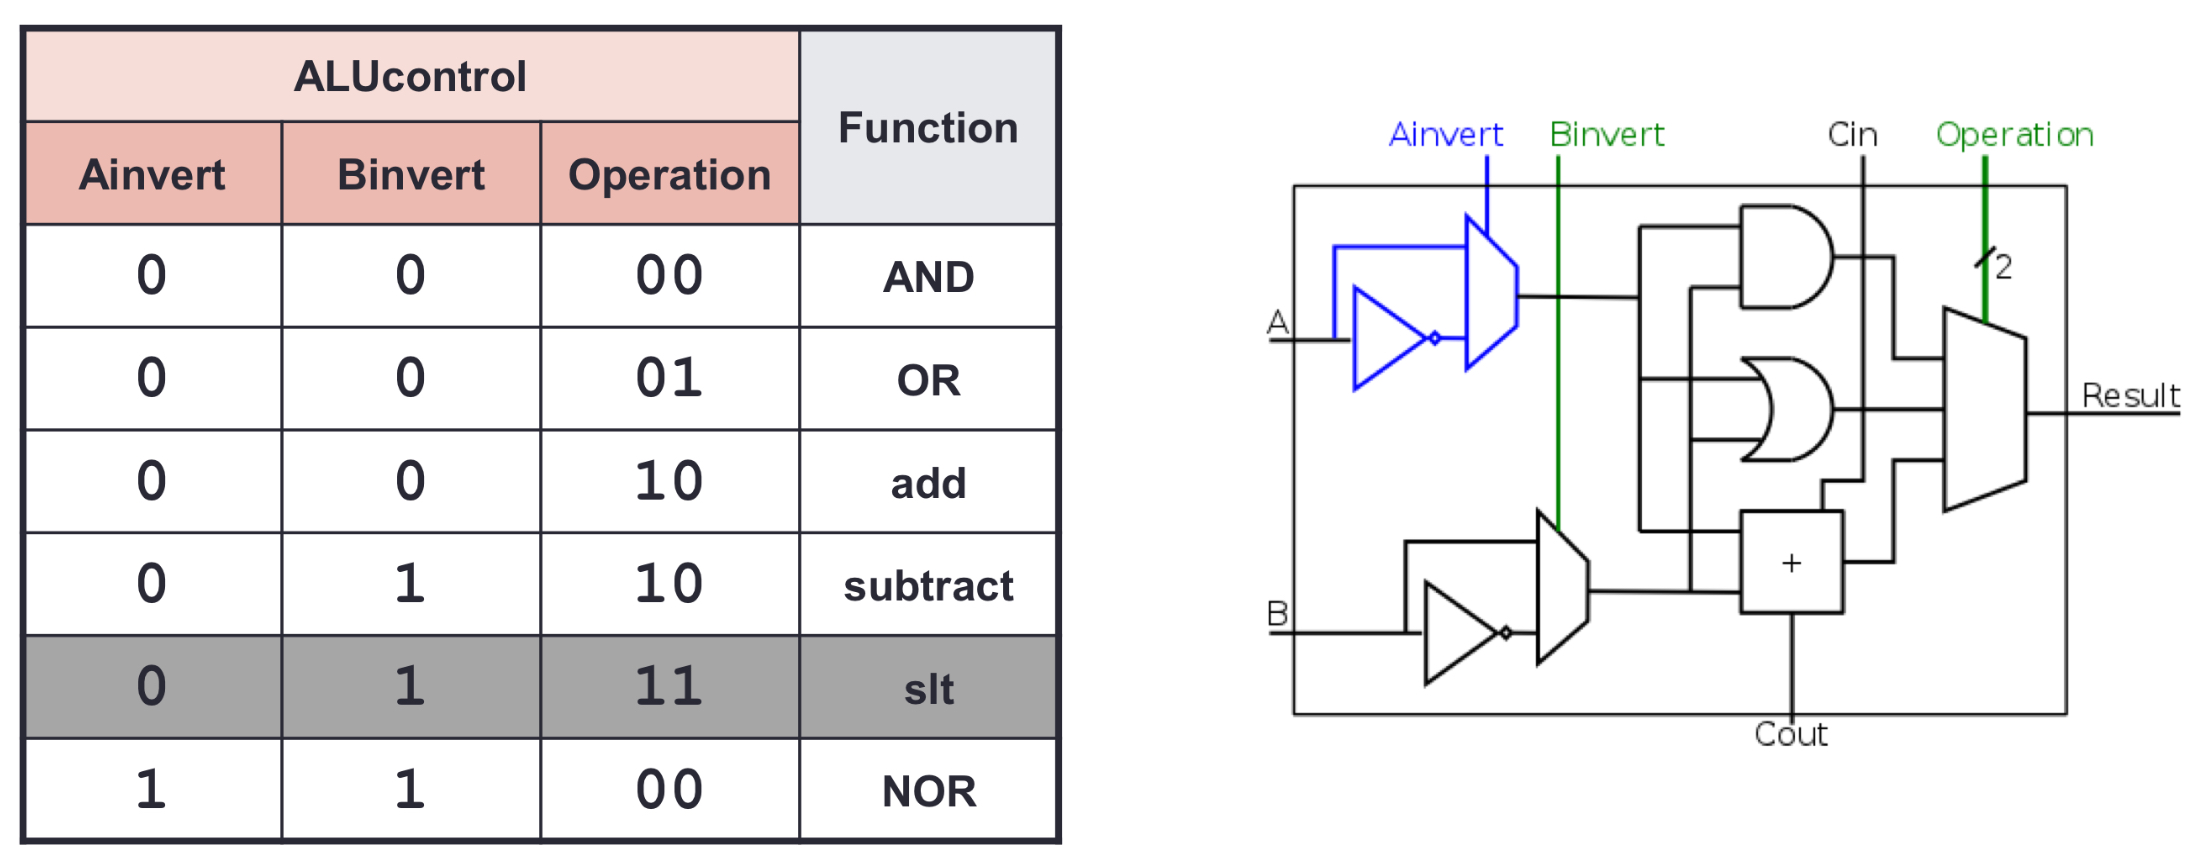
\includegraphics[width=0.7\textwidth]{aluControl2.jpeg}
\end{figure}

We can design the ALUControl signal which depends on the opcode and function
code fields with a \textit{multilevel decoding approach}, by generating an
intermediate signal \verb|ALUop| from the 6-bit opcode, and then obtain
\verb|ALUcontrol| from \verb|ALUop| and funct.

\begin{remark}
  The multilevel decoding approach simplifies the design process, reduces the
  size of the main controller, and potentially speeds up the circuit.
\end{remark}

\begin{figure}[h!]
  \centering
  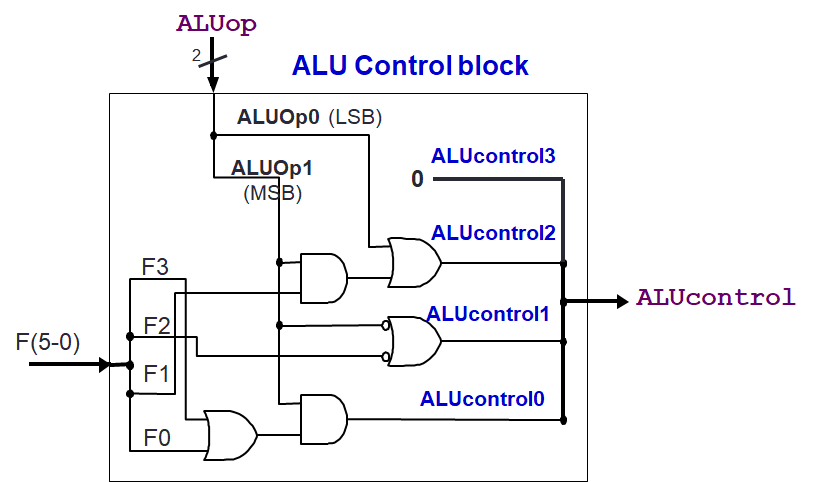
\includegraphics[width=0.5\textwidth]{aluControlCircuit.png}
\end{figure}

\begin{figure*}[h!]
  \centering
  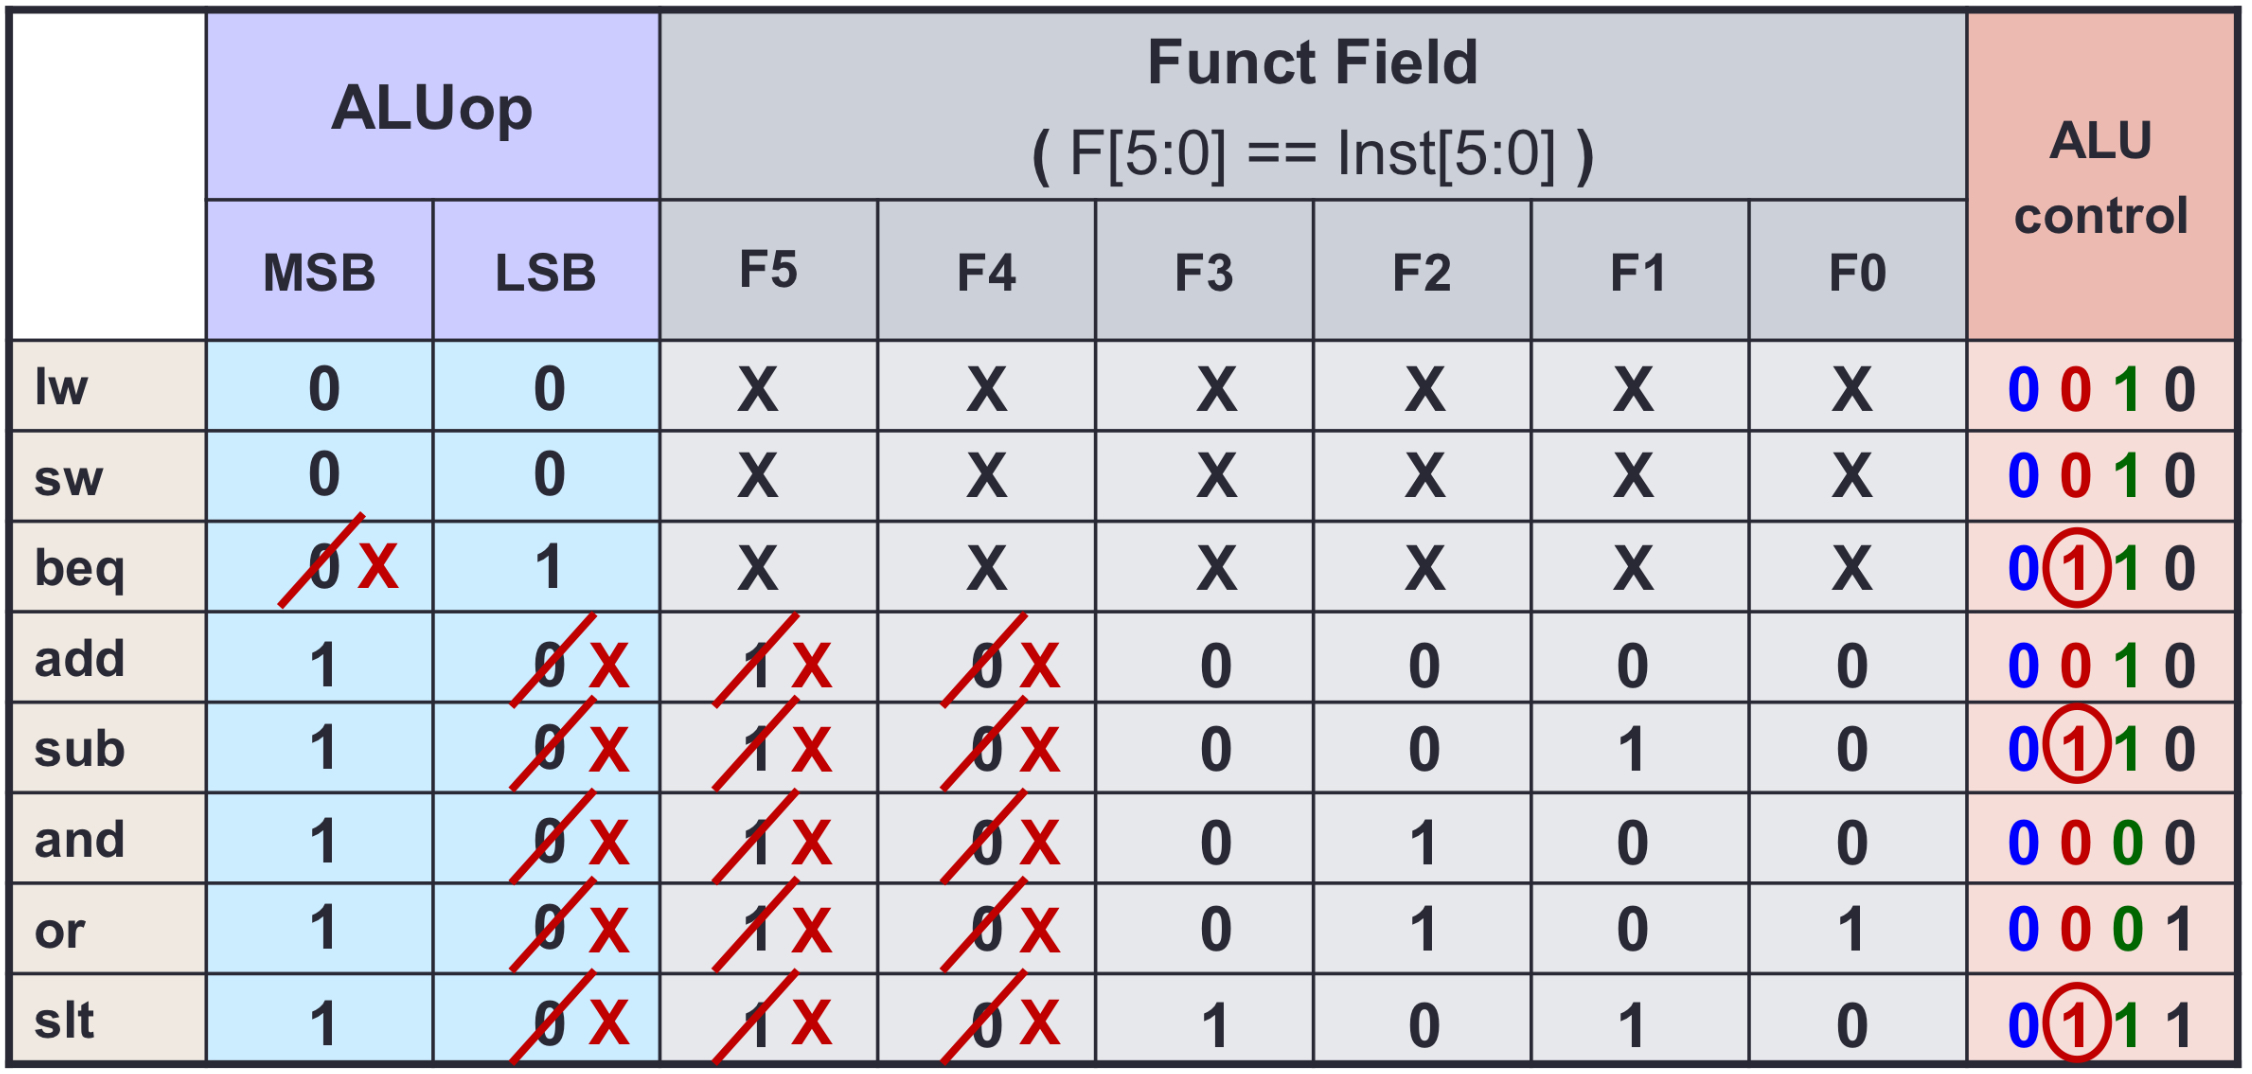
\includegraphics[width=0.65\textwidth]{aluControlOverview.jpeg}
  \captionsetup{labelformat=empty}
  \caption{ALUop $\to$ ALUcontrol}
\end{figure*}

\paragraph{Control Design}
With the required outputs of the control, we now design the control circuit using the
opcode.
\begin{figure}[h!]
  \centering
  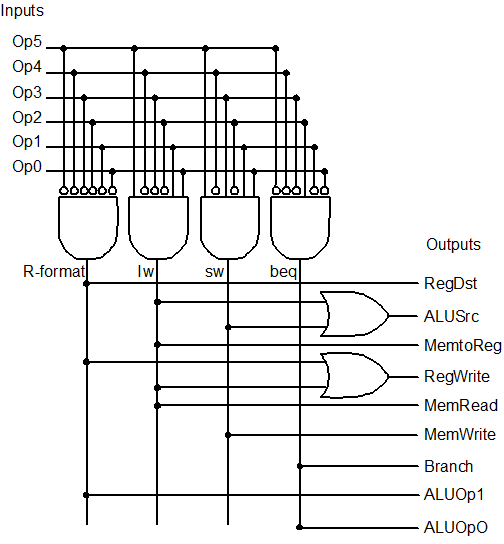
\includegraphics[width=0.4\textwidth]{controlCircuit.png}
\end{figure}
\begin{figure}[h!]
  \centering
  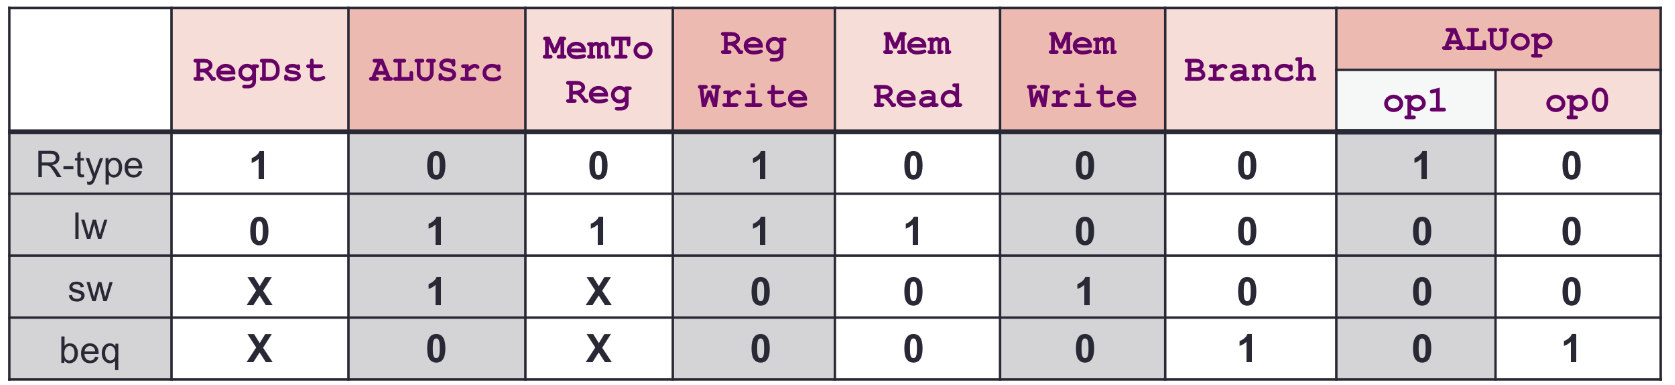
\includegraphics[width=0.7\textwidth]{control.jpeg}
  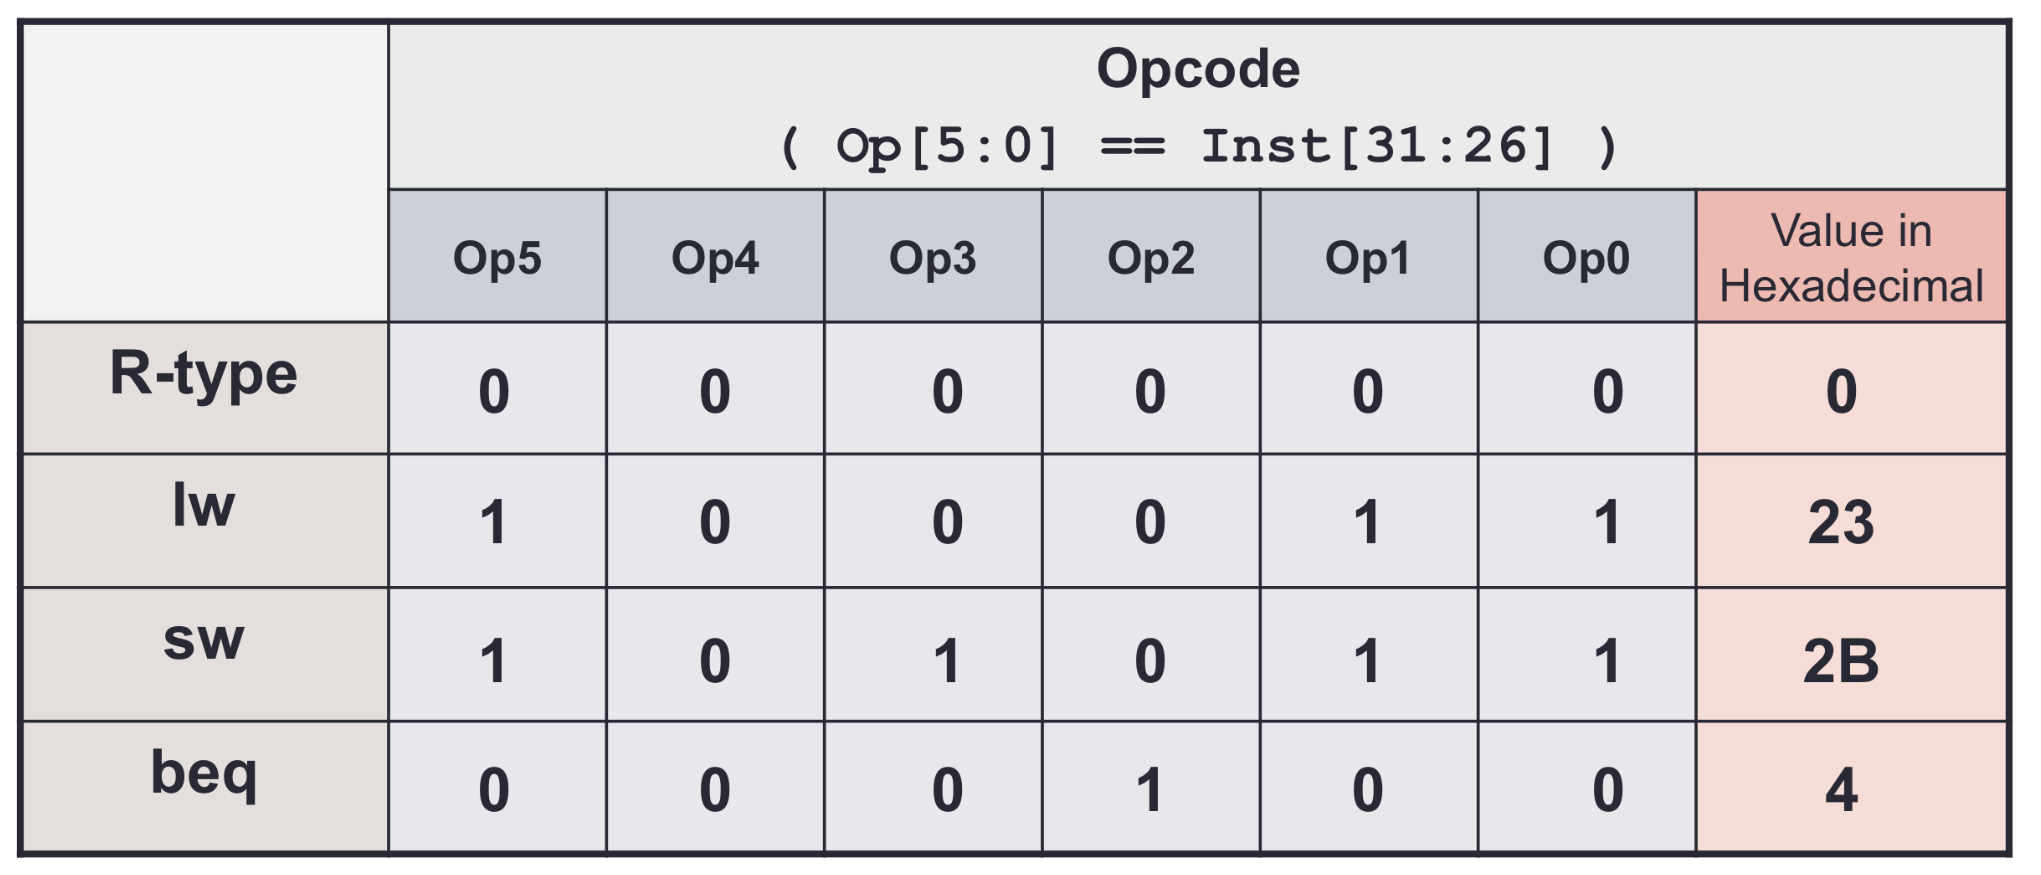
\includegraphics[width=0.4\textwidth]{control2.jpeg}
  \captionsetup{labelformat=empty}
  \caption{opcode $\to$ Control Signals}
\end{figure}

\subsection{Instruction Execution}
Each instruction consists of three phases: \textit{Read} contents of one or
more storage elements, Perform \textit{computations} through some combinational
logic, \textit{Write} results to one or more storage elements.

Each instruction is performed within a single \textbf{clock period}. The clock
period is used to prevent concurrent reading and writing to the storage
elements.
\begin{figure}[h!]
  \centering
  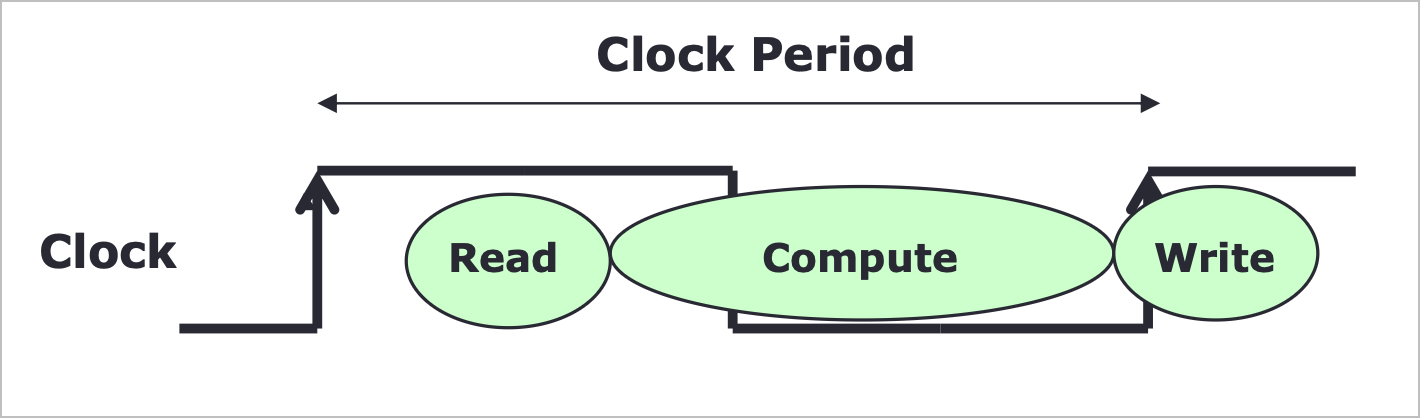
\includegraphics[width=0.5\textwidth]{clockPeriod.png}
\end{figure}

The clock period is computed based on the instructions to be executed, and has
multiple possible implementations.

\subsubsection{Single Cycle Implementation}
In Single Cycle Implementation, we calculate the clock cycle time based on the
slowest instruction between \textit{ALU}, \textit{lw}, \textit{sw},
\textit{beq} instructions.
\begin{example}
  Assuming neglligible delays, we have the total time for each instruction:
  \begin{figure}[h!]
    \centering
    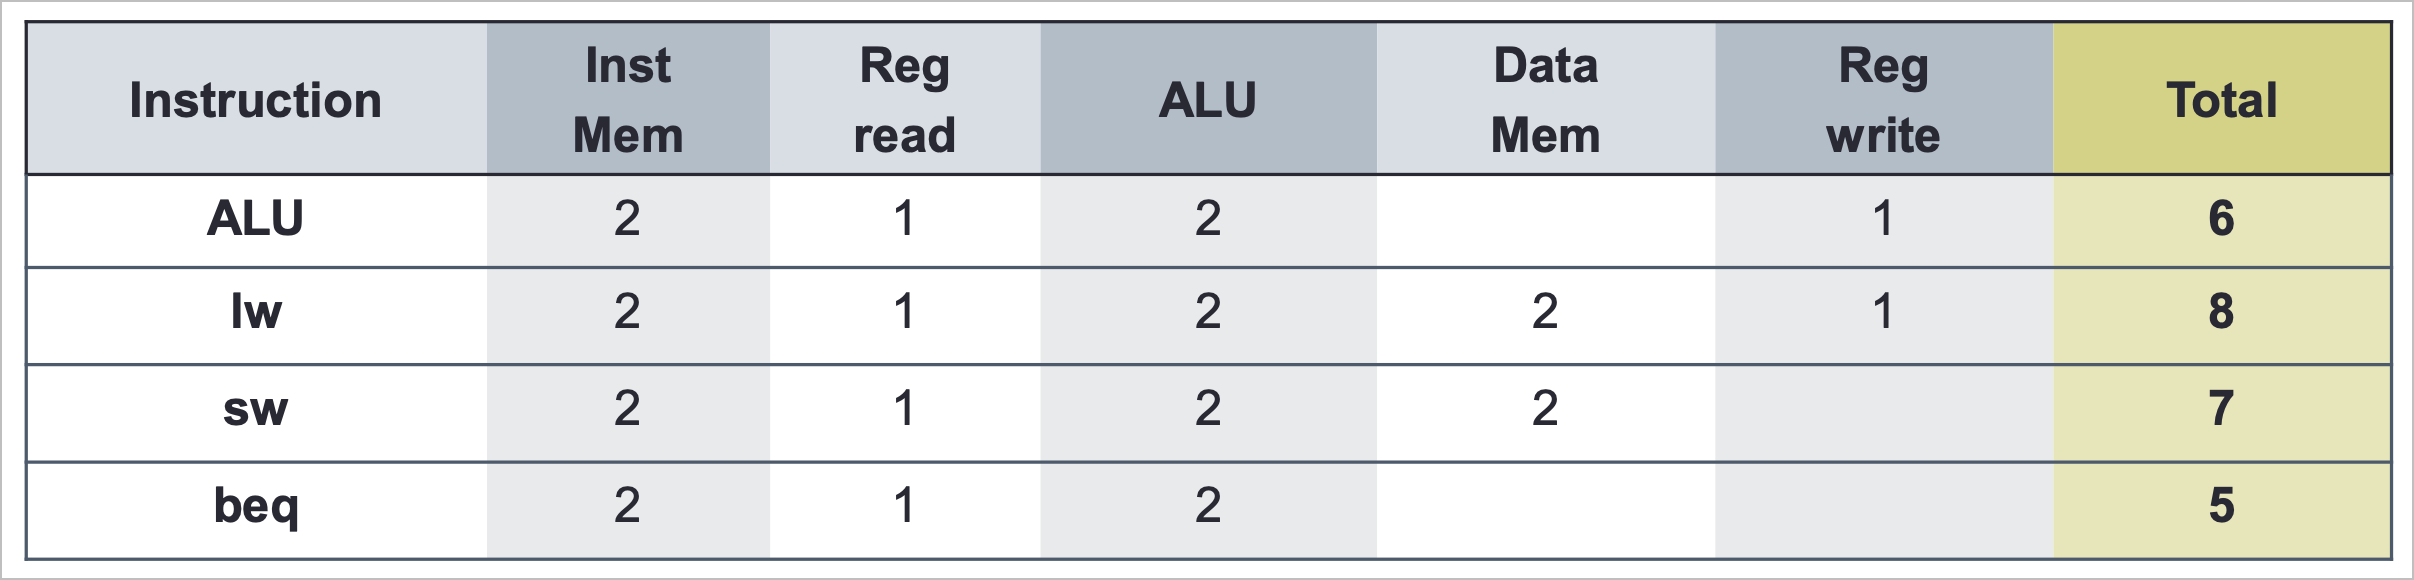
\includegraphics[width=0.6\textwidth]{singleCycle.png}
  \end{figure}
\end{example}
Implementing a single cycle for all instructions, each instruction will take as
much time as the slowest one.
  
\subsubsection{Multicycle Implementation}
In multicycle implementation, we break up instructions into \textit{execution
steps}, each taking a single clock cycle.
\begin{itemize}
  \item Instruction Fetch
  \item Instruction Decode and Register Read
  \item ALU Operation
  \item Memory Read/Write
  \item Register Write
\end{itemize}
The cycle time is hence much shorter, and each instruction takes a variable
number of clock cycles.

\subsubsection{Pipelining}
In addition to breaking up instructions into execution steps, we may
\textit{allow different instructions to be in different execution steps
simultaneously}. This is known as \textbf{pipelining}.

\newpage
\begin{sideways}[h!]
  \centering
  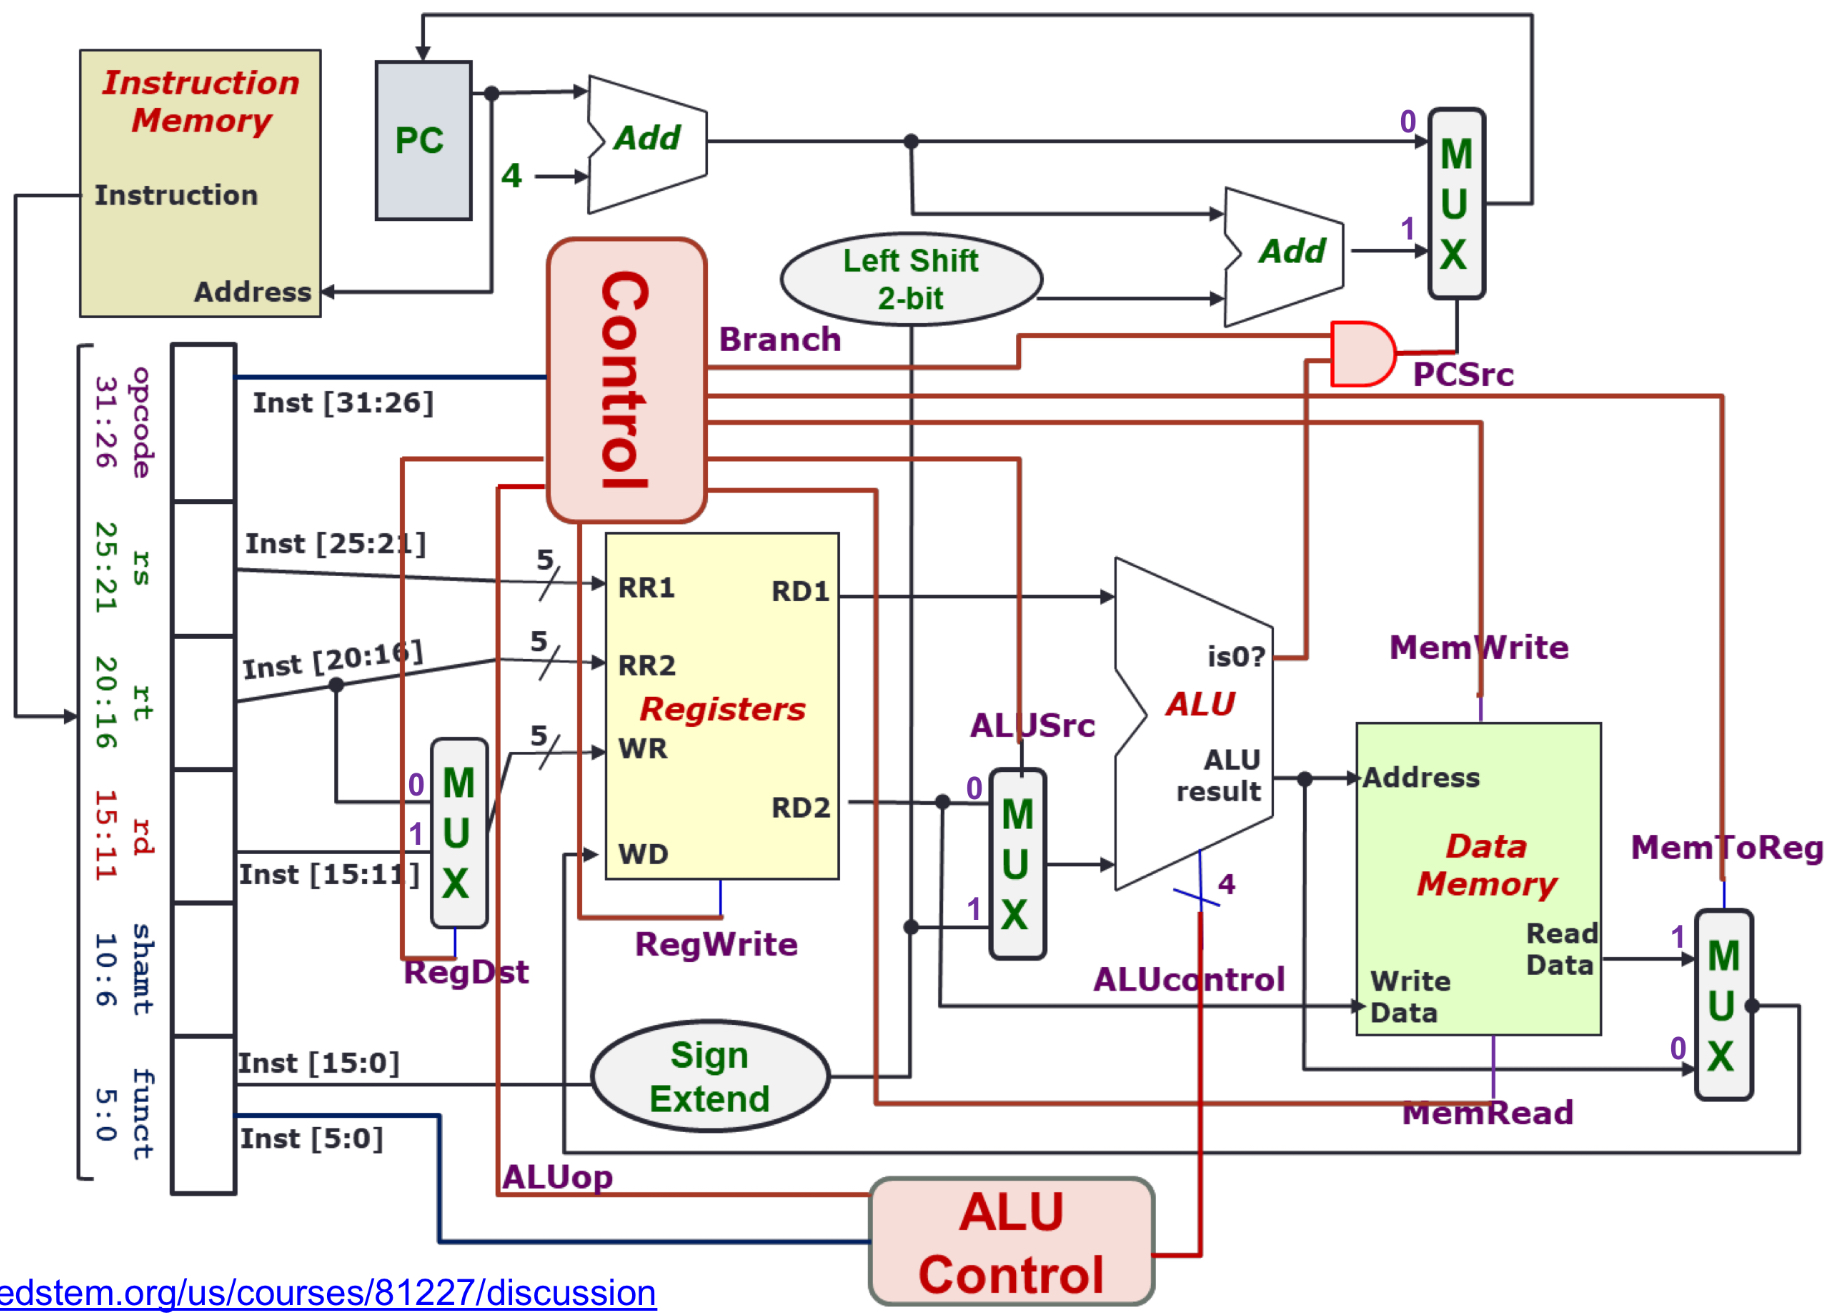
\includegraphics[width=1.35\textwidth]{processor.jpeg}
\end{sideways}
\newpage

\section{Circuit Design}
\paragraph{Circuit Types}
We focus on digital circuits design with the advantages over analog circuits:
\begin{itemize}
  \item More reliable, with simpler circuits and less noise-prone
  \item Specified accuracy (determinable)
  \item Abstraction can be applied using boolean algebra
  \item Simpler design, analysis and simplification
\end{itemize}
Among digital circuits, we have \textit{combinational circuits} (with no
memory, and output depends solely on the input) and \textit{sequential
circuits} (where output depends on both input and current state of memory).

\subsection{Boolean Algebra}
\subsubsection{Operations}
\begin{notation}
  In Boolean Algebra, True is denoted as $T$ or $1$, and False as $F$ or $0$.
  We denote conjunction (AND) as $A\cdot B$ or $A\wedge B$, disjunction (OR) as
  $A+B$ or $A\vee B$, and negation (NOT) as $A'$, $\bar{A}$ or $\neg{A}$. 
  \begin{remark}
    In CS2100, we use $1$ for True, $0$ for false, $\cdot$ for conjunction, $+$
    for disjunction and $'$ for negation.
  \end{remark}
\end{notation}
\paragraph{Precedence of Operators}
There is no convention for boolean algebra in general. We define the precedence
of operators from higher to lowest (for CS2100):
\begin{enumerate}
  \item Not ($'$)
  \item And ($\cdot$)
  \item Or ($+$)
\end{enumerate}
\subsubsection{Results of Boolean Algebra}
We have the following laws of boolean algebra:

\centering
\begin{tabular}{c c c}
  \toprule
  Law & Disjunction & Conjunction\\
  \midrule
  Identity Laws & $A+0=0+A=A$ & $A\cdot 1=1\cdot A = A$ \\
  Inverse/Complement Laws & $A+A'=A'+A=1$ & $A\cdot A'=A'\cdot A=0$ \\
  Commutative Laws & $A+B=B+A$ & $A\cdot B=B\cdot A$ \\
  Associative Laws & $A+(B+C)=(A+B)+C$ & $A\cdot(B\cdot C)=(A\cdot B)\cdot C$ \\
  Distributive Laws & $A\cdot (B+C)=(A\cdot B)+(A\cdot C)$ & $A+(B\cdot C)=(A+B)\cdot(A+C)$ \\
  \bottomrule
\end{tabular}\\
\vspace{4mm}
\raggedright%
and the following theorems:\\
\vspace{2mm}

\centering
\begin{tabular}{c c c}
  \toprule
  Theorem & Disjunction & Conjunction \\
  \midrule
  Idempotency & $X+X=X$ & $X\cdot X=X$ \\
  One Element / Zero Element & $X+1=1$ & $X\cdot 0 = 0$ \\
  Involution & \multicolumn{2}{c}{$\left( X' \right)'=X $ } \\
  Absorption 1 & $X+X\cdot Y=X$ & $X\cdot (X+Y)=X$ \\
  Absorption 2 & $X+X'\cdot Y=X+Y$ & $X\cdot (X'+Y)=X\cdot Y$ \\
  De Morgan's Laws & $(X+Y)'=X'\cdot Y'$ & $(X\cdot Y)'=X'+Y'$ \\
  \multirow{2}{4em}{Consensus} & \multicolumn{2}{c}{$X\cdot Y+X'\cdot Z + Y\cdot Z=X\cdot Y+X'\cdot Z$}\\
  & \multicolumn{2}{c}{$(X+Y)\cdot(X'+Z)\cdot(Y+Z)=(X+Y)\cdot(X'+Z)$} \\
  \bottomrule
\end{tabular}

\raggedright%
\paragraph{Duality} Each result comes in pairs. If each AND/OR operator and
identity element 0/1 in a boolean equation is interchanged, it remains valid. This
is known as \textit{duality}.

\subsubsection{Standard Forms}
\paragraph{Definitions}
\begin{definition}[Terms]
  A boolean variable, or its complemented form is known as a \textit{literal}.
  A single literal, or a logical product (AND) of literals is a \textit{product
  term}. Similarly, a single literal, or a logical sum (OR) of literals is a
  \textit{sum term}.
\end{definition}
We define two standard forms of boolean expressions, to the end of desirable
circuits for implementation:
\begin{itemize}
  \item \textit{Sum-of-Products (SOP)}: A product term, or a logical sum (OR) of several product terms.
  \item \textit{Product-of-Sums (POS)}: A sum term, or a logical product (AND) of several sum terms.
\end{itemize}
\begin{remark}
  All boolean expressions can be expressed in SOP and POS form.
\end{remark}
\begin{definition}[Minterm, Maxterm]
  A \textit{minterm} of $x$ variables is a product term containing $x$
  literals, denoted m0 to m$(2^{n}-1)$. A \textit{maxterm} of $x$ variables is a
  sum term containing $x$ literals, denoted M0 to M$(2^{n}-1)$.
\end{definition}
\begin{example}[Number of min-, maxterms]
  Given $n$ variables, we have up to $2^{n}$ minterms and $2^{n}$ maxterms.
  \begin{figure}[h!]
    \centering
    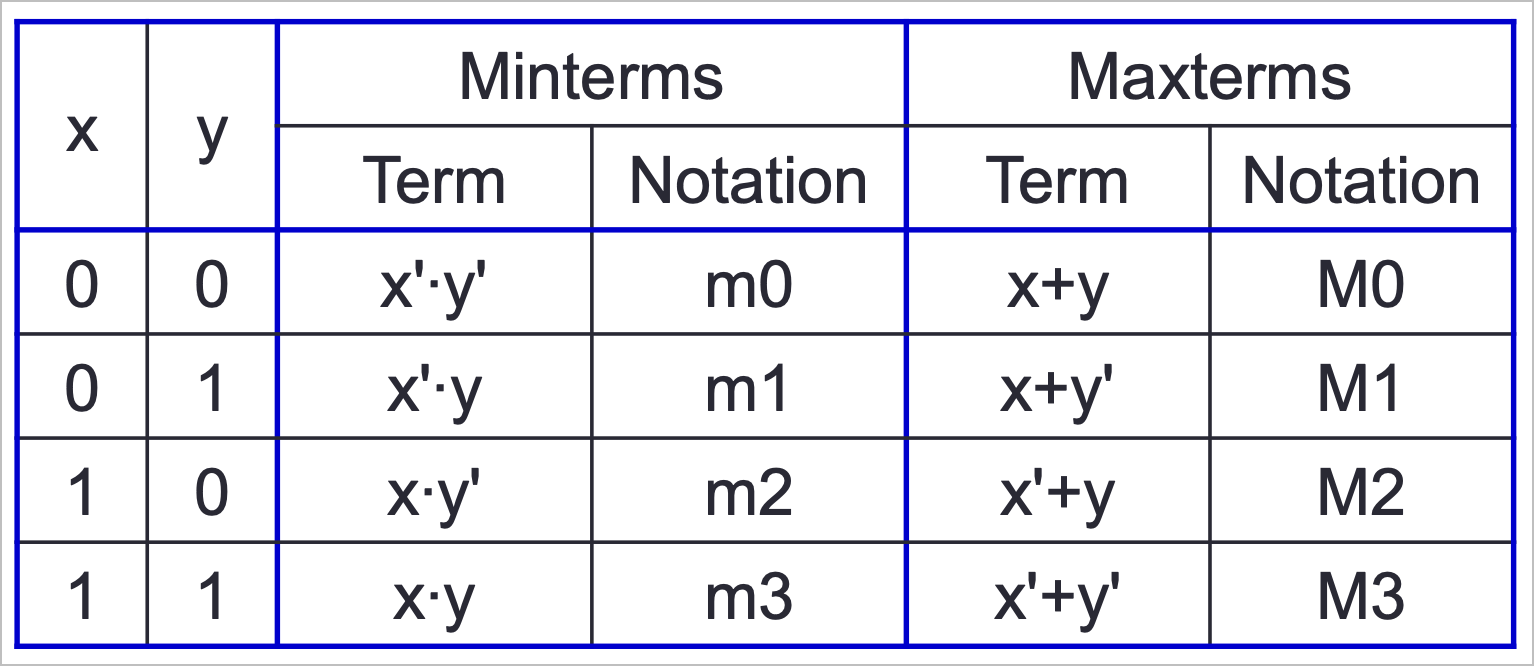
\includegraphics[width=0.5\textwidth]{minMaxTerms.png}
  \end{figure}
\end{example}
\textbf{Each minterm is the complement of the corresponding maxterm.}
To find the m(x) minterm, where $x={(b_1b_2\cdots b_{n})}_2$, we have the
product of $n$ literals of which each literal $a_i=\begin{cases}a_i'&b_i=0\\a_i&b_i=1\end{cases}$. The M(x) maxterm is then the sum of $n$ literals where
each literal $a_i =\begin{cases}a_i&b_i=0\\a_i'&b=1\end{cases}$

Using minterms and maxterms, we may then obtain a \textbf{canonical/normal
form}, which ensures uniqueness of the SOP or POS\@.

A \textit{sum-of-minterms} is the canonical SOP, denoted $\sum m(k_1,k_2,\ldots
k_i)$. It can be obtained by gathering the minterms with which the output is 1.
A \textit{product-of-maxterms} is the canonical POS, denoted $\prod
M(k_1,k_2,\ldots,k_i)$. It can be obtained by gathering the maxterms with which
the output is 0.

Additionally, each function $F=\sum m(k_1,k_2,\ldots,k_i)=\prod M(l_1,l_2,\ldots,l_j)$
where $\left\{ 0,\ldots,n-1 \right\}\setminus\left\{ k_1,k_2,\ldots k_i
\right\}=\left\{ l_1,l_2,\ldots l_j \right\} $.


\subsection{Circuit Simplification}
Given a boolean expression, we may then simplify to obtain a circuit that uses
fewer logic gates, such that it is cheaper, uses less power and (sometimes)
faster. We do this with various simplification techniques, namely
\textbf{algebraic simplification}, \textbf{Karnaugh Maps}, and
the \textbf{Quine-McCluskey Technique}.

\subsubsection{Algebraic Simplification}
By application of the boolean algebra results and theorems, we are able to
minimise the number of literals and number of terms. However, these two
minimisations may sometimes be in conflict, in which case we have to opt to
adapt the tradeoff within the constraints in our context. \\

Algebraic manipulation allows us to adapt the technique, but is sometimes
challenging, requiring strong algebraic manipulation skills.

\subsubsection{Karnaugh Maps}
\begin{definition}[Gray Code]
  An ordering of the binary numerals is a \textit{Gray code} if every two
  successive values differ in only one bit.
\end{definition}
A Gray code is an unweighted code, and every of the $n$-bits are usually
utilised to have a sequence of $2^n$ values. The $n$-bit standard gray code can
be obtained inductively from the $(n-1)$-bit standard gray code.
\begin{figure}[h!]
  \centering
  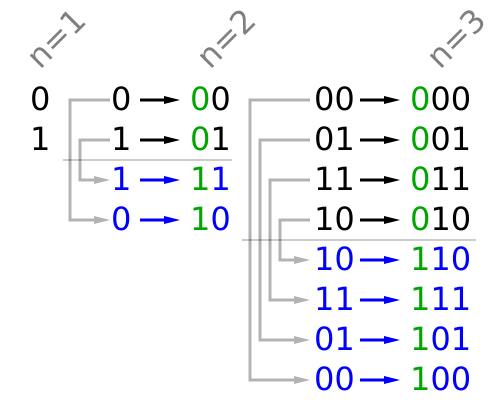
\includegraphics[width=0.26\textwidth]{gray_code}
\end{figure}\\
Given $n$-bits, there are multiple possible Gray code cycles, from which the
standard Gray code uniquely specifies one. For instance, we have the $4$-bit
standard gray code as shown.
\begin{figure}[h!]
  \centering
  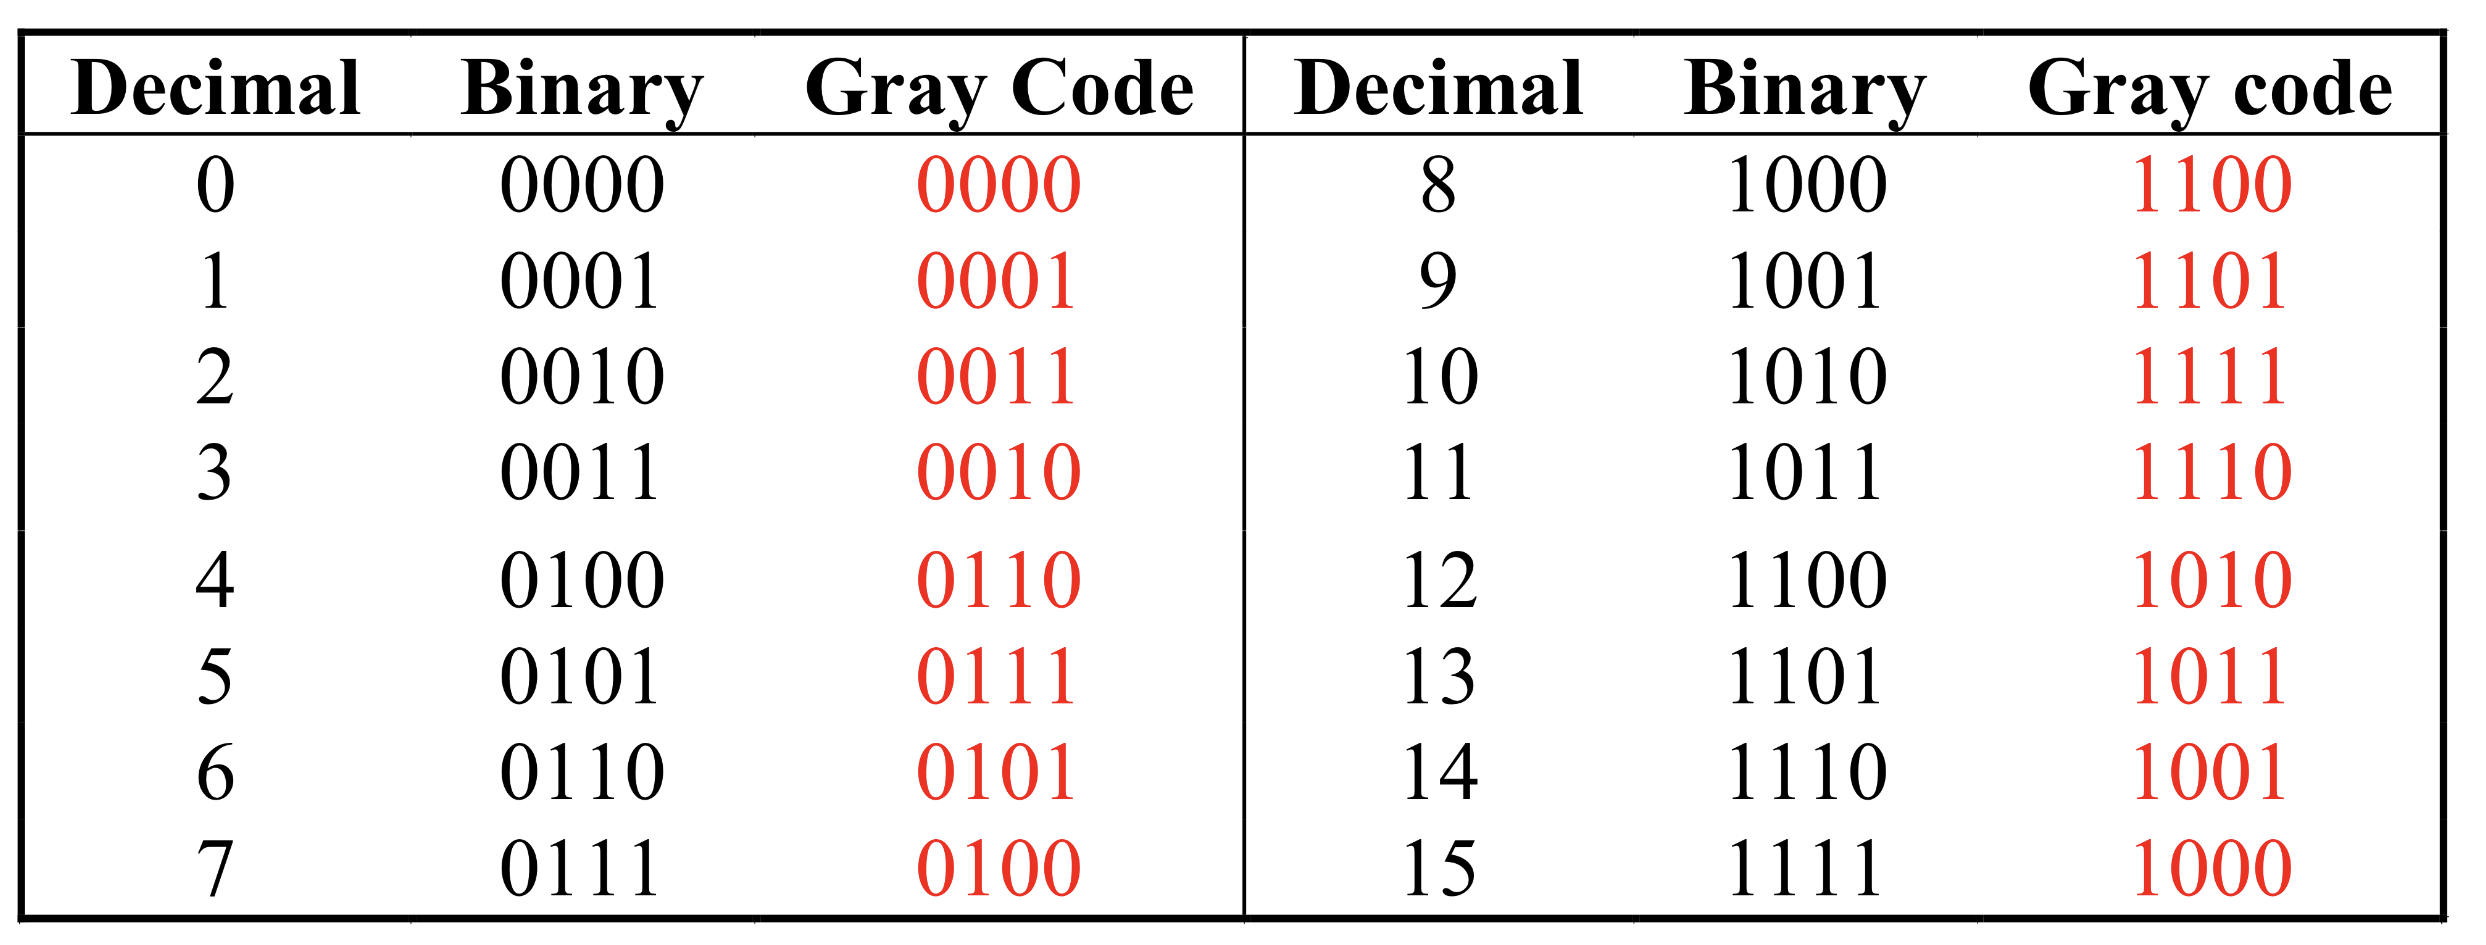
\includegraphics[width=0.5\textwidth]{4_gray_code}
\end{figure}\\
Within a universal set $U$ of minterms, we can partition the minterms, from
which a boolean function is a subset where we obtain the SOP expression. We may
use venn diagrams to analyse boolean expressions.
\begin{definition}[Karnaugh Maps]
  A \textit{K-Map} is an abstract form of a Venn diagram organised as a matrix
  of cells where
  \begin{itemize}
    \item Each cell represents a minterm
    \item Adjacents cell differ by one literal
  \end{itemize}
\end{definition}
We define K-maps up to 6 variables. For each K-map, we fill each cell with $1$
if it corresponds to a minterm of the function, $d$ if it corresponds to a
dont-care term, and $0$ otherwise. Given an arbitrary Boolean function, we can
convert it to a SOP form, where we can then fill the K-map directly, or
construct the truth table to obtain the minterms.
\paragraph{n-Variable K-Maps} Given n variables $a,b$, we have the K-maps as
shown below, with axes each Gray codes representing the status of the
variables, and where each cell has n neighbours.
\begin{figure}[h!]
  \centering
  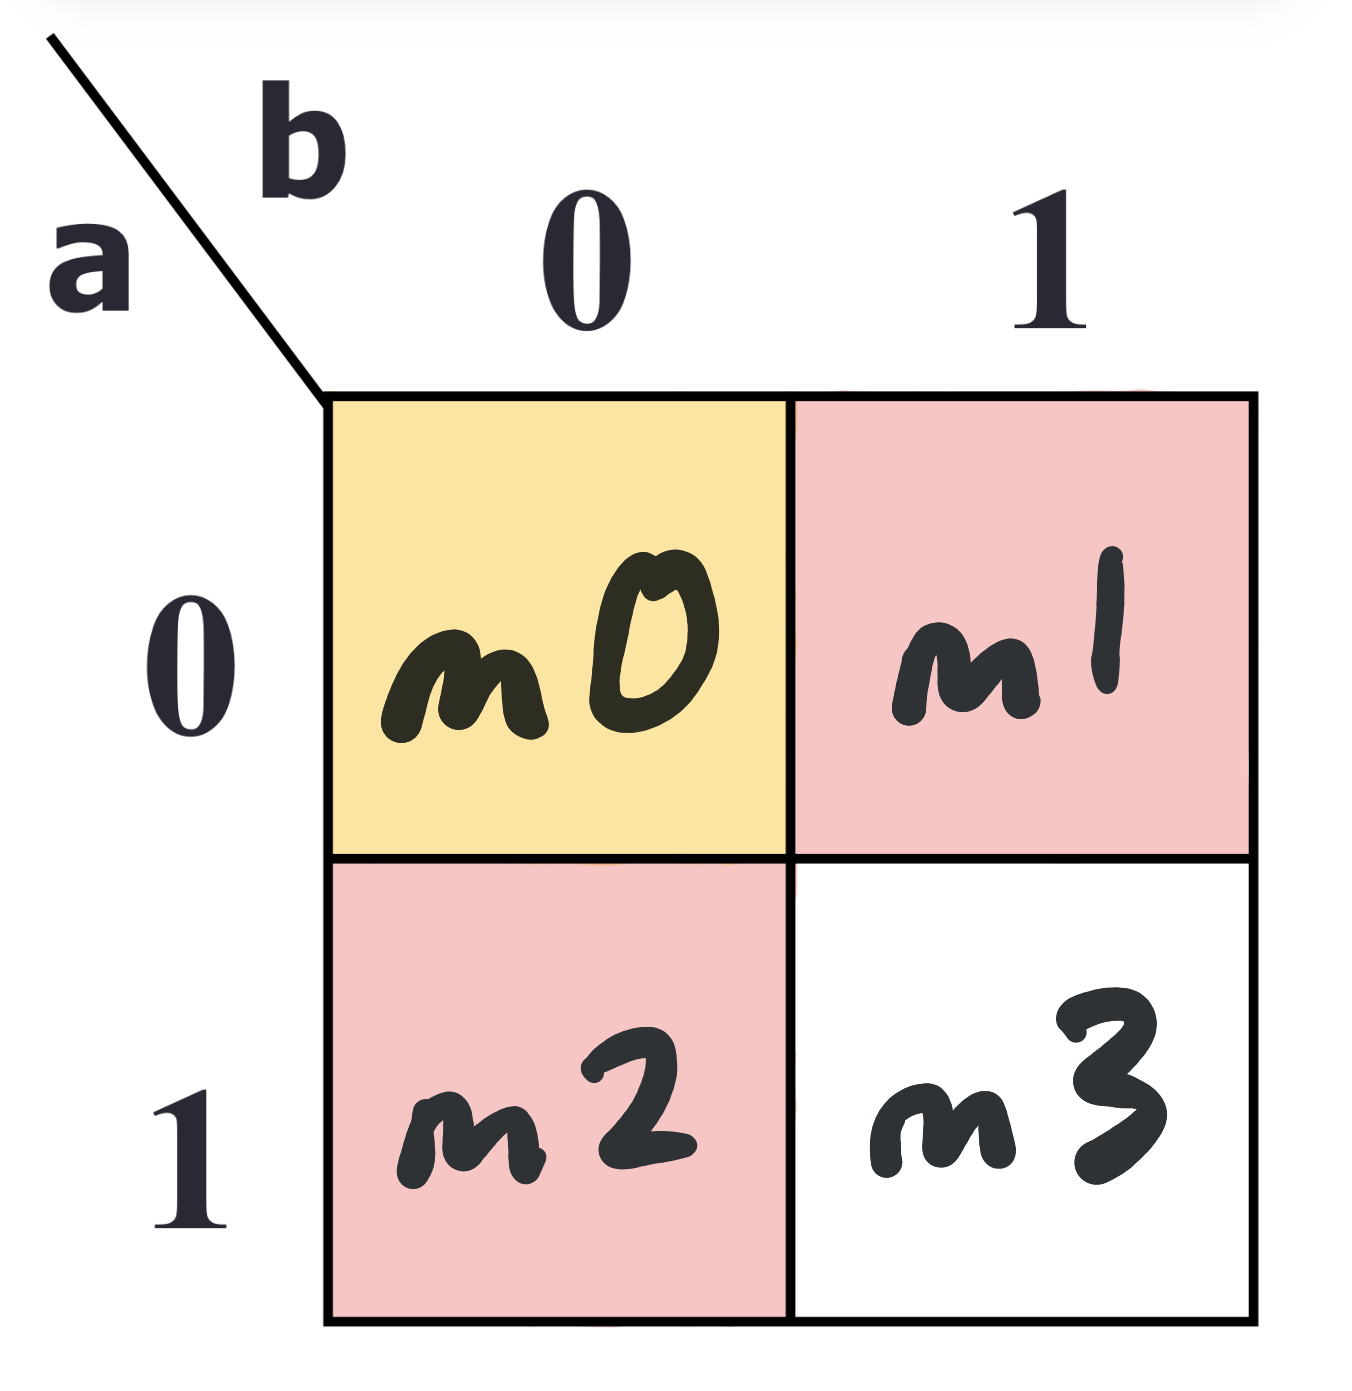
\includegraphics[width=0.15\textwidth]{kmap2}
  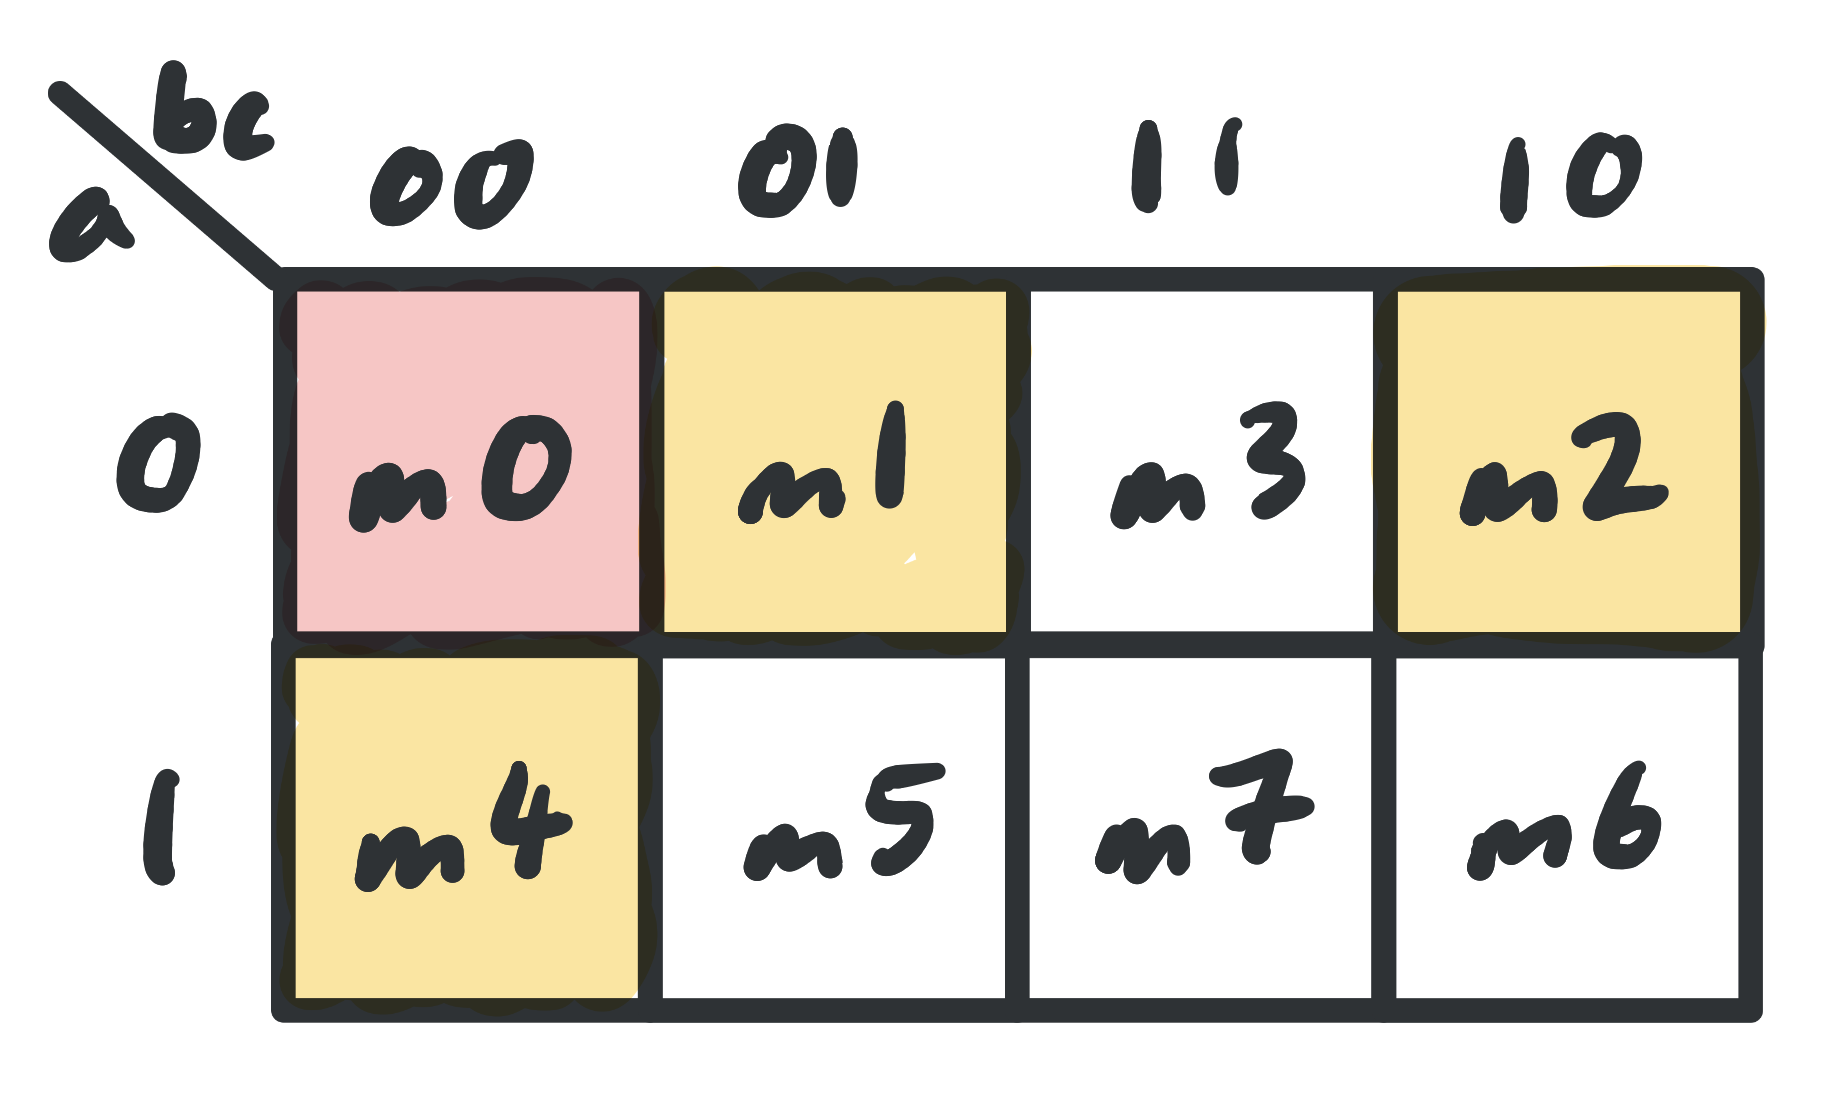
\includegraphics[width=0.25\textwidth]{kmap3}
\end{figure}
\begin{figure}[h!]
  \centering
  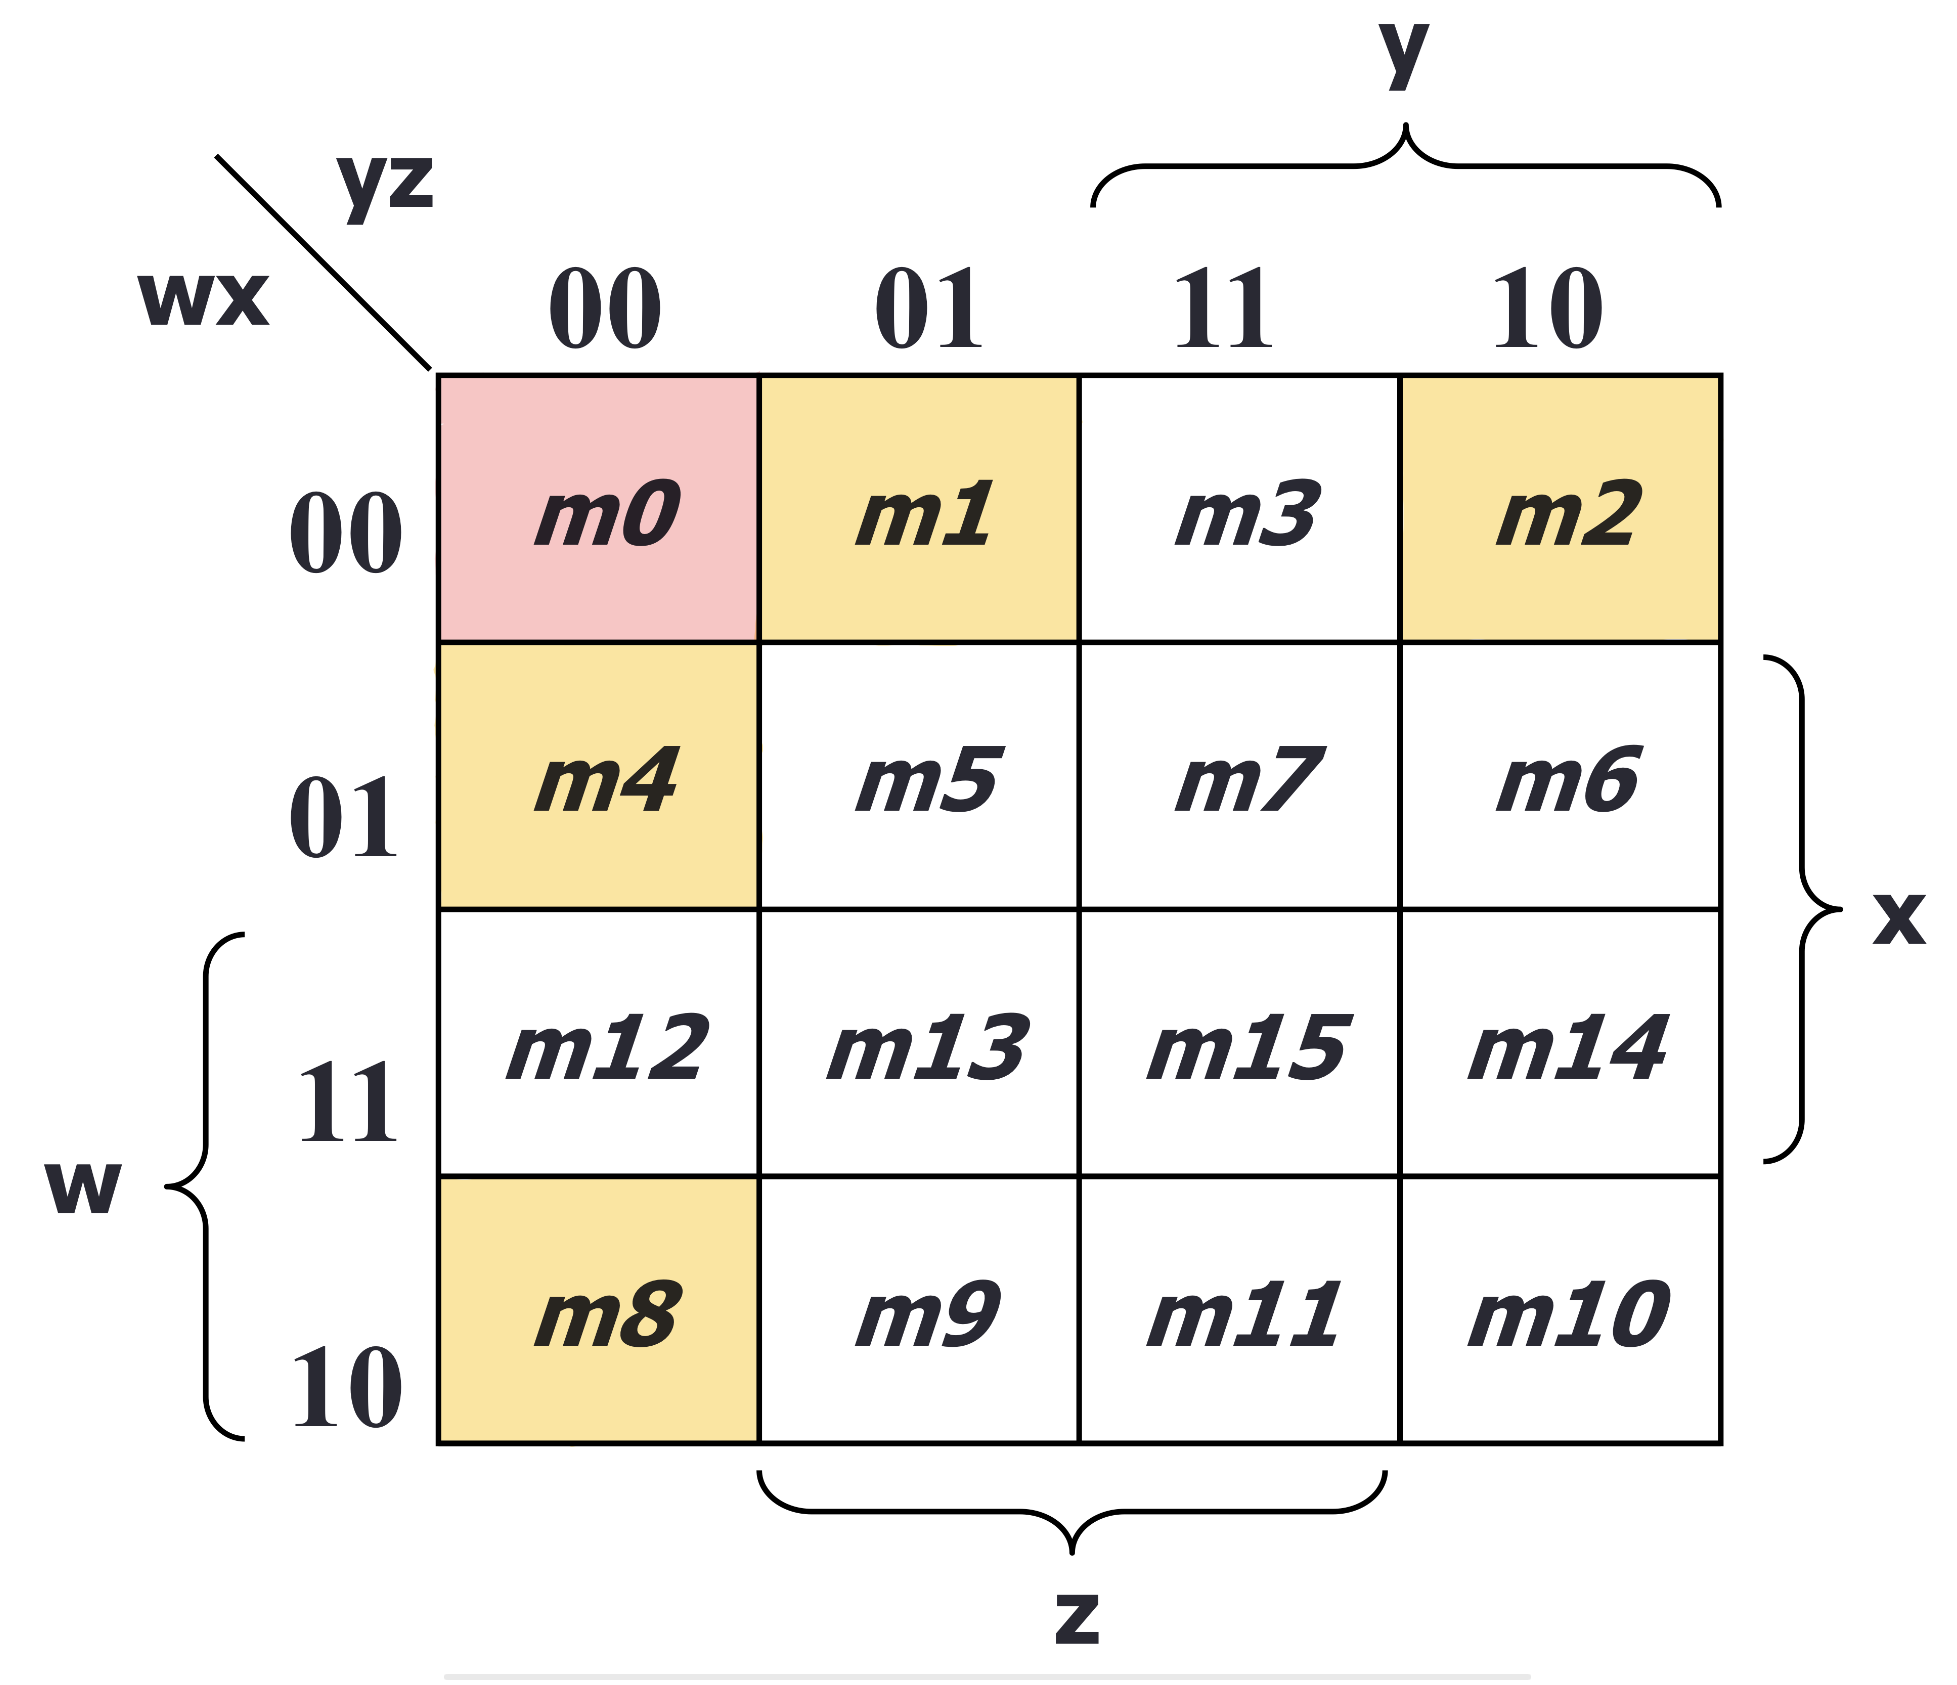
\includegraphics[width=0.4\textwidth]{kmap4}
\end{figure}\\
\begin{figure}[h!]
  \centering
  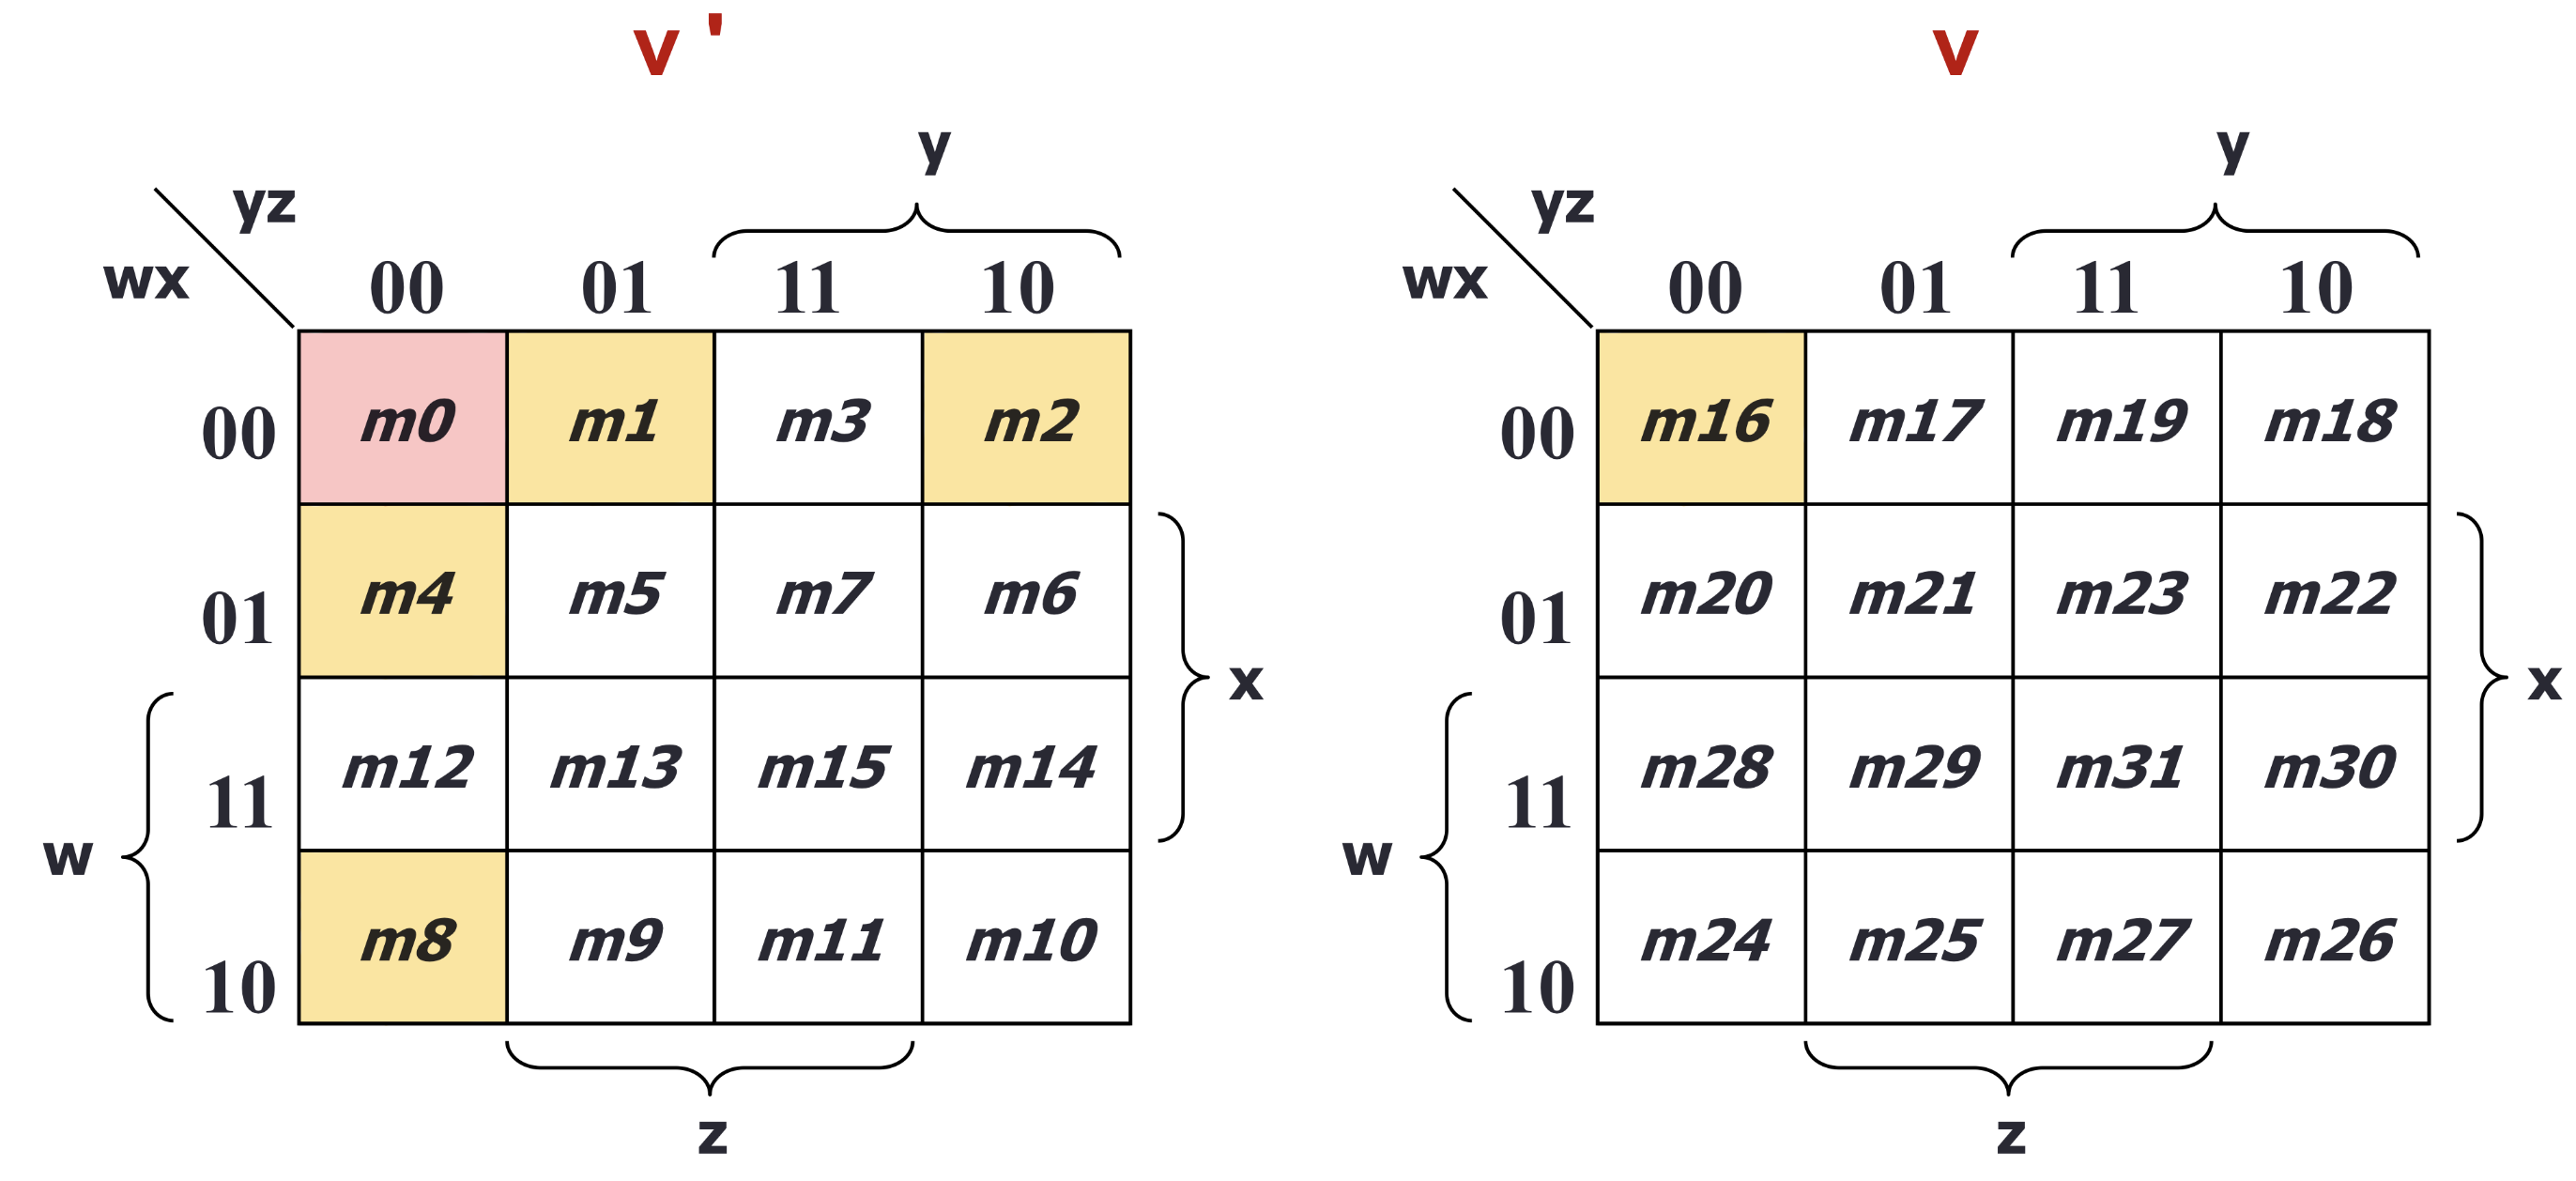
\includegraphics[width=0.73\textwidth]{kmap5}
\end{figure}
\begin{figure}[h!]
  \centering
  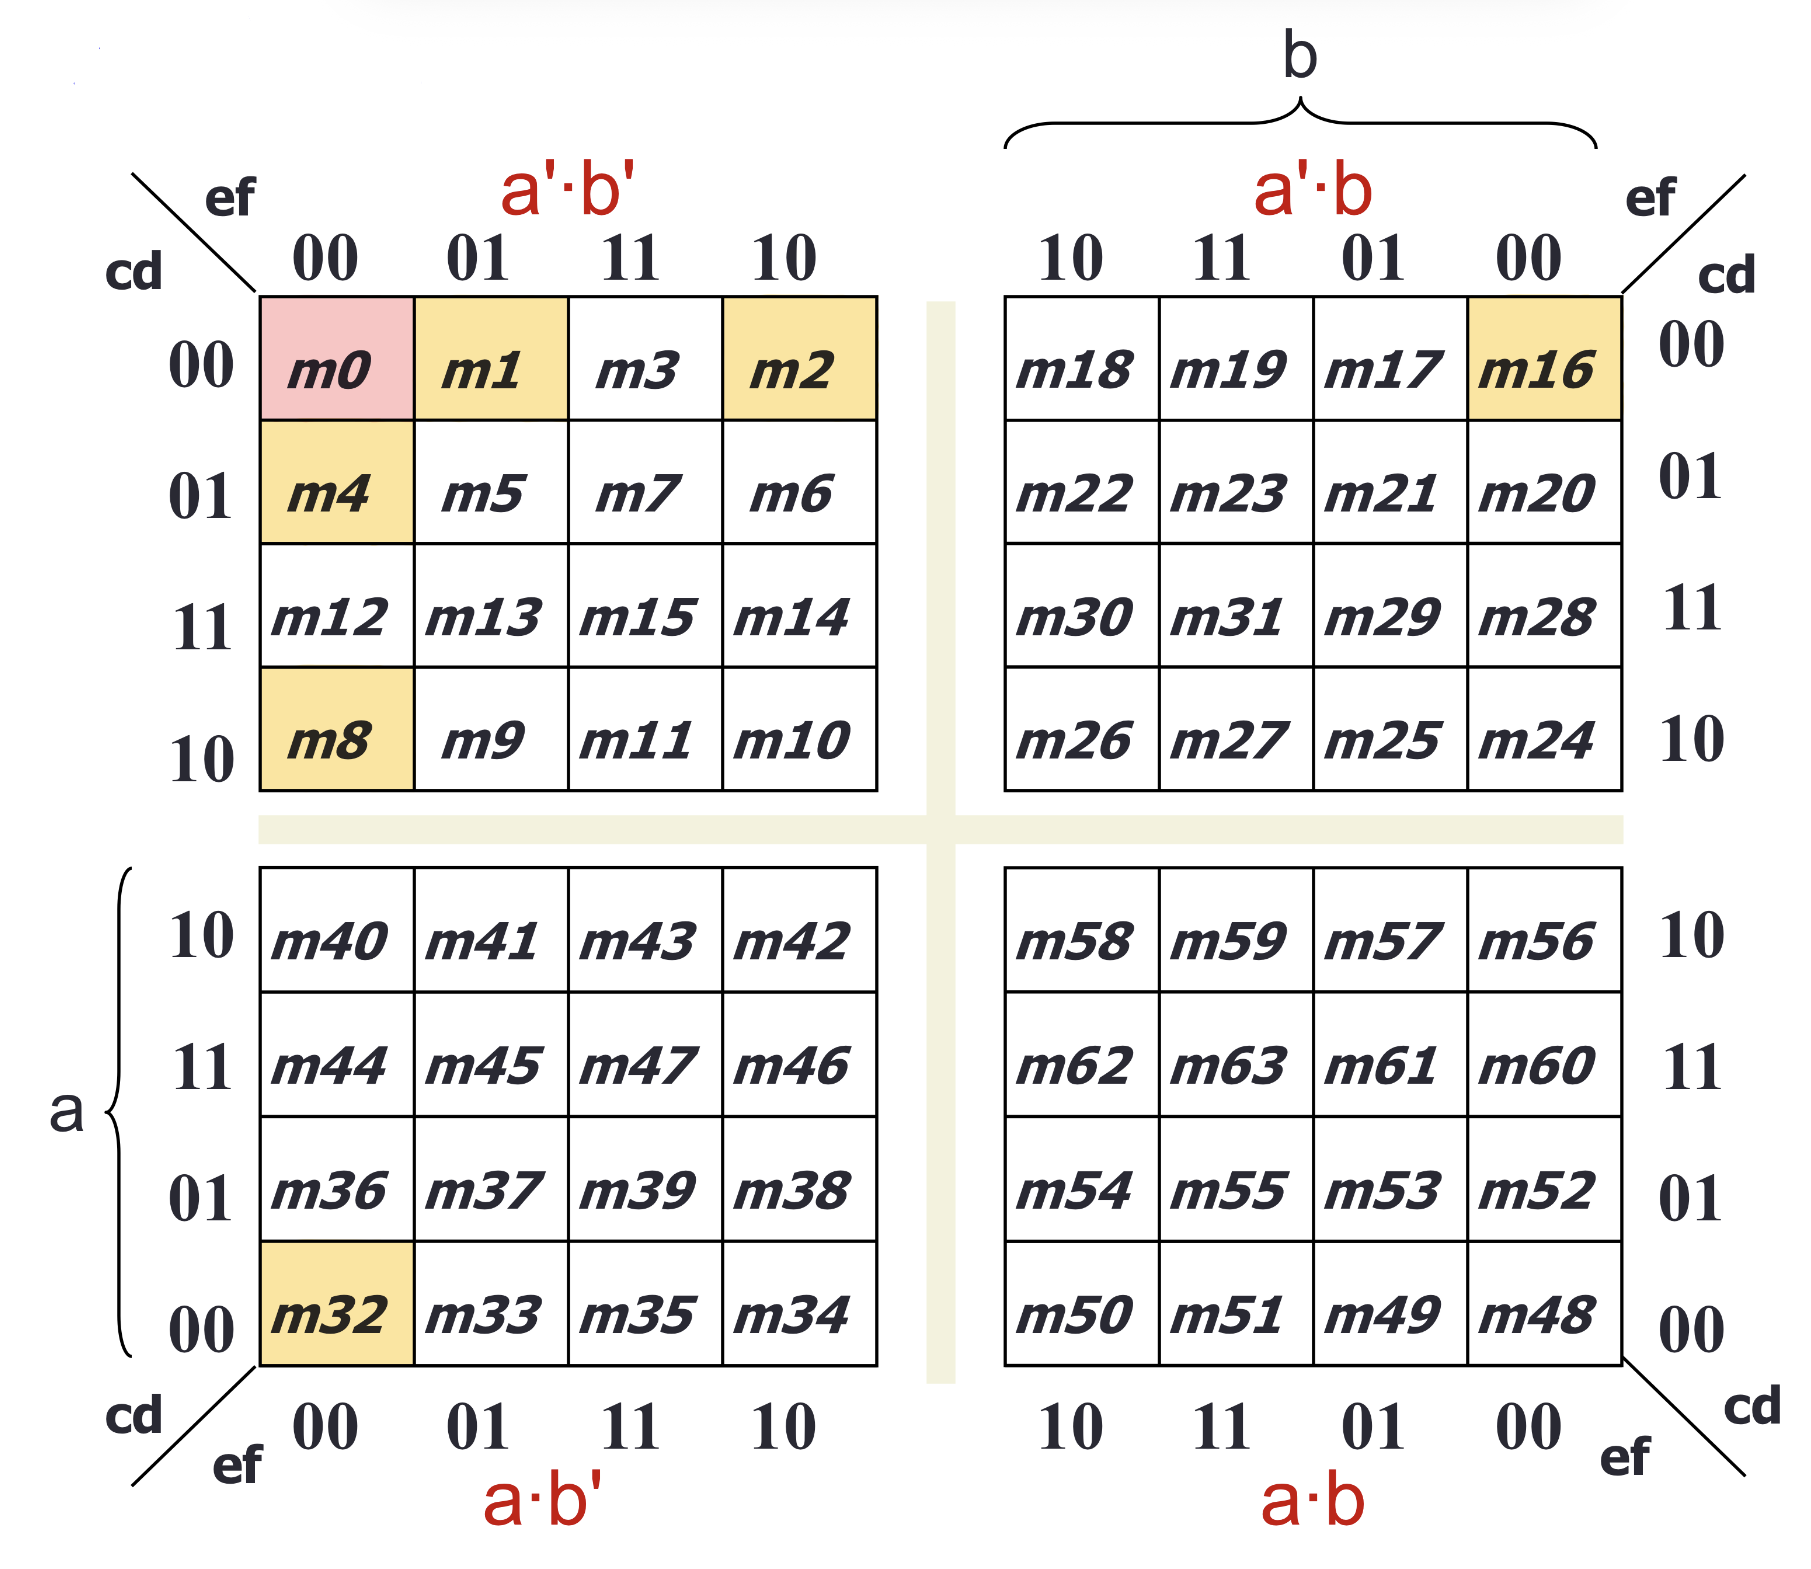
\includegraphics[width=0.5\textwidth]{kmap6}
\end{figure}
\vspace{16mm}
Given a filled K-map, we may obtain valid groupings of adjacent cells as follows:
\begin{itemize}
  \item Each cell may be grouped with any of its neighbouring cell
  \item Each group has size in powers of two
  \item Each group correspond to a product term
  \item Each don't-care term can be taken to be $1$ or $0 $ to obtain a simpler
    expression
\end{itemize}
\begin{remark}
  Each grouping of $2^{n}$ cells eliminates $n$ variables from the product
  terms.
\end{remark}
\begin{definition}[Prime Implicants]
  A product term that is obtained by combining the maximum number of minterms
  from adjacent squares in the map is known as a \textit{prime implicant}.
\end{definition}
\begin{definition}[Essential Prime Implicant]
  A prime implicant that includes at least one minterm that is not covered by
  any other prime implicant is known as a \textit{essential prime implicant}.
\end{definition}
Given the K-map, we may then find a \textbf{simplified SOP expression} to the
function with the following algorithm.
\begin{enumerate}
  \item Identify PIs of the function by finding all largest possible groupings.
  \item Within the PIs, identify the EPIs that must exist in the expression.
  \item Select a minimum subset of the remaining PIs to complete the cover.
\end{enumerate}

Alternatively, we may find a \textbf{simplified POS expression} to the function
by grouping the maxterms. This is equivalent to grouping the minterms in the
K-map of the function's complement. We can then obtain the POS expression by
taking the inverse of the SOP expression found from this grouping.\\

By using K-Maps, we can minimise the number of product terms and literals. They
are easy to use, but limits us to 5 to 6 variables.


\subsubsection{Quine-McCluskey Technique}
With $n$ variables, in the Quine-McCluskey Technique, we denote each product
term as a $n$-length string, with $1, 0$ for the literals, and $-$ for an
absence of a variable. We can obtain a simplified expression using an iterative
algorithm. Given a sum-of-minterms expression, 
\begin{enumerate}
  \item Arrange the terms in groups according to the number of $1$s.
  \item Combine terms from adjacent groups which differ by only $1$ bit.
  \item Iterate step $2$ until no further combinations are possible.
\end{enumerate}
When terms are combined, we indicate them as such with a tick. When the program
terminates, terms that have not been combined are the PIs. We then find a cover
using a PI chart, to find the EPIs given by columns with a single $X$, and then
a reduced PI chart to find a minimum cover for the remaining minterms.
\begin{example}
  Given a $4$-variable function
  \[F(A,B,C,D)=\sum m\left( 2,4,6,8,9,10,12,13,15 \right)\] 
  we have the following table from applying the algorithm.
  \begin{figure}[h!]
    \centering
    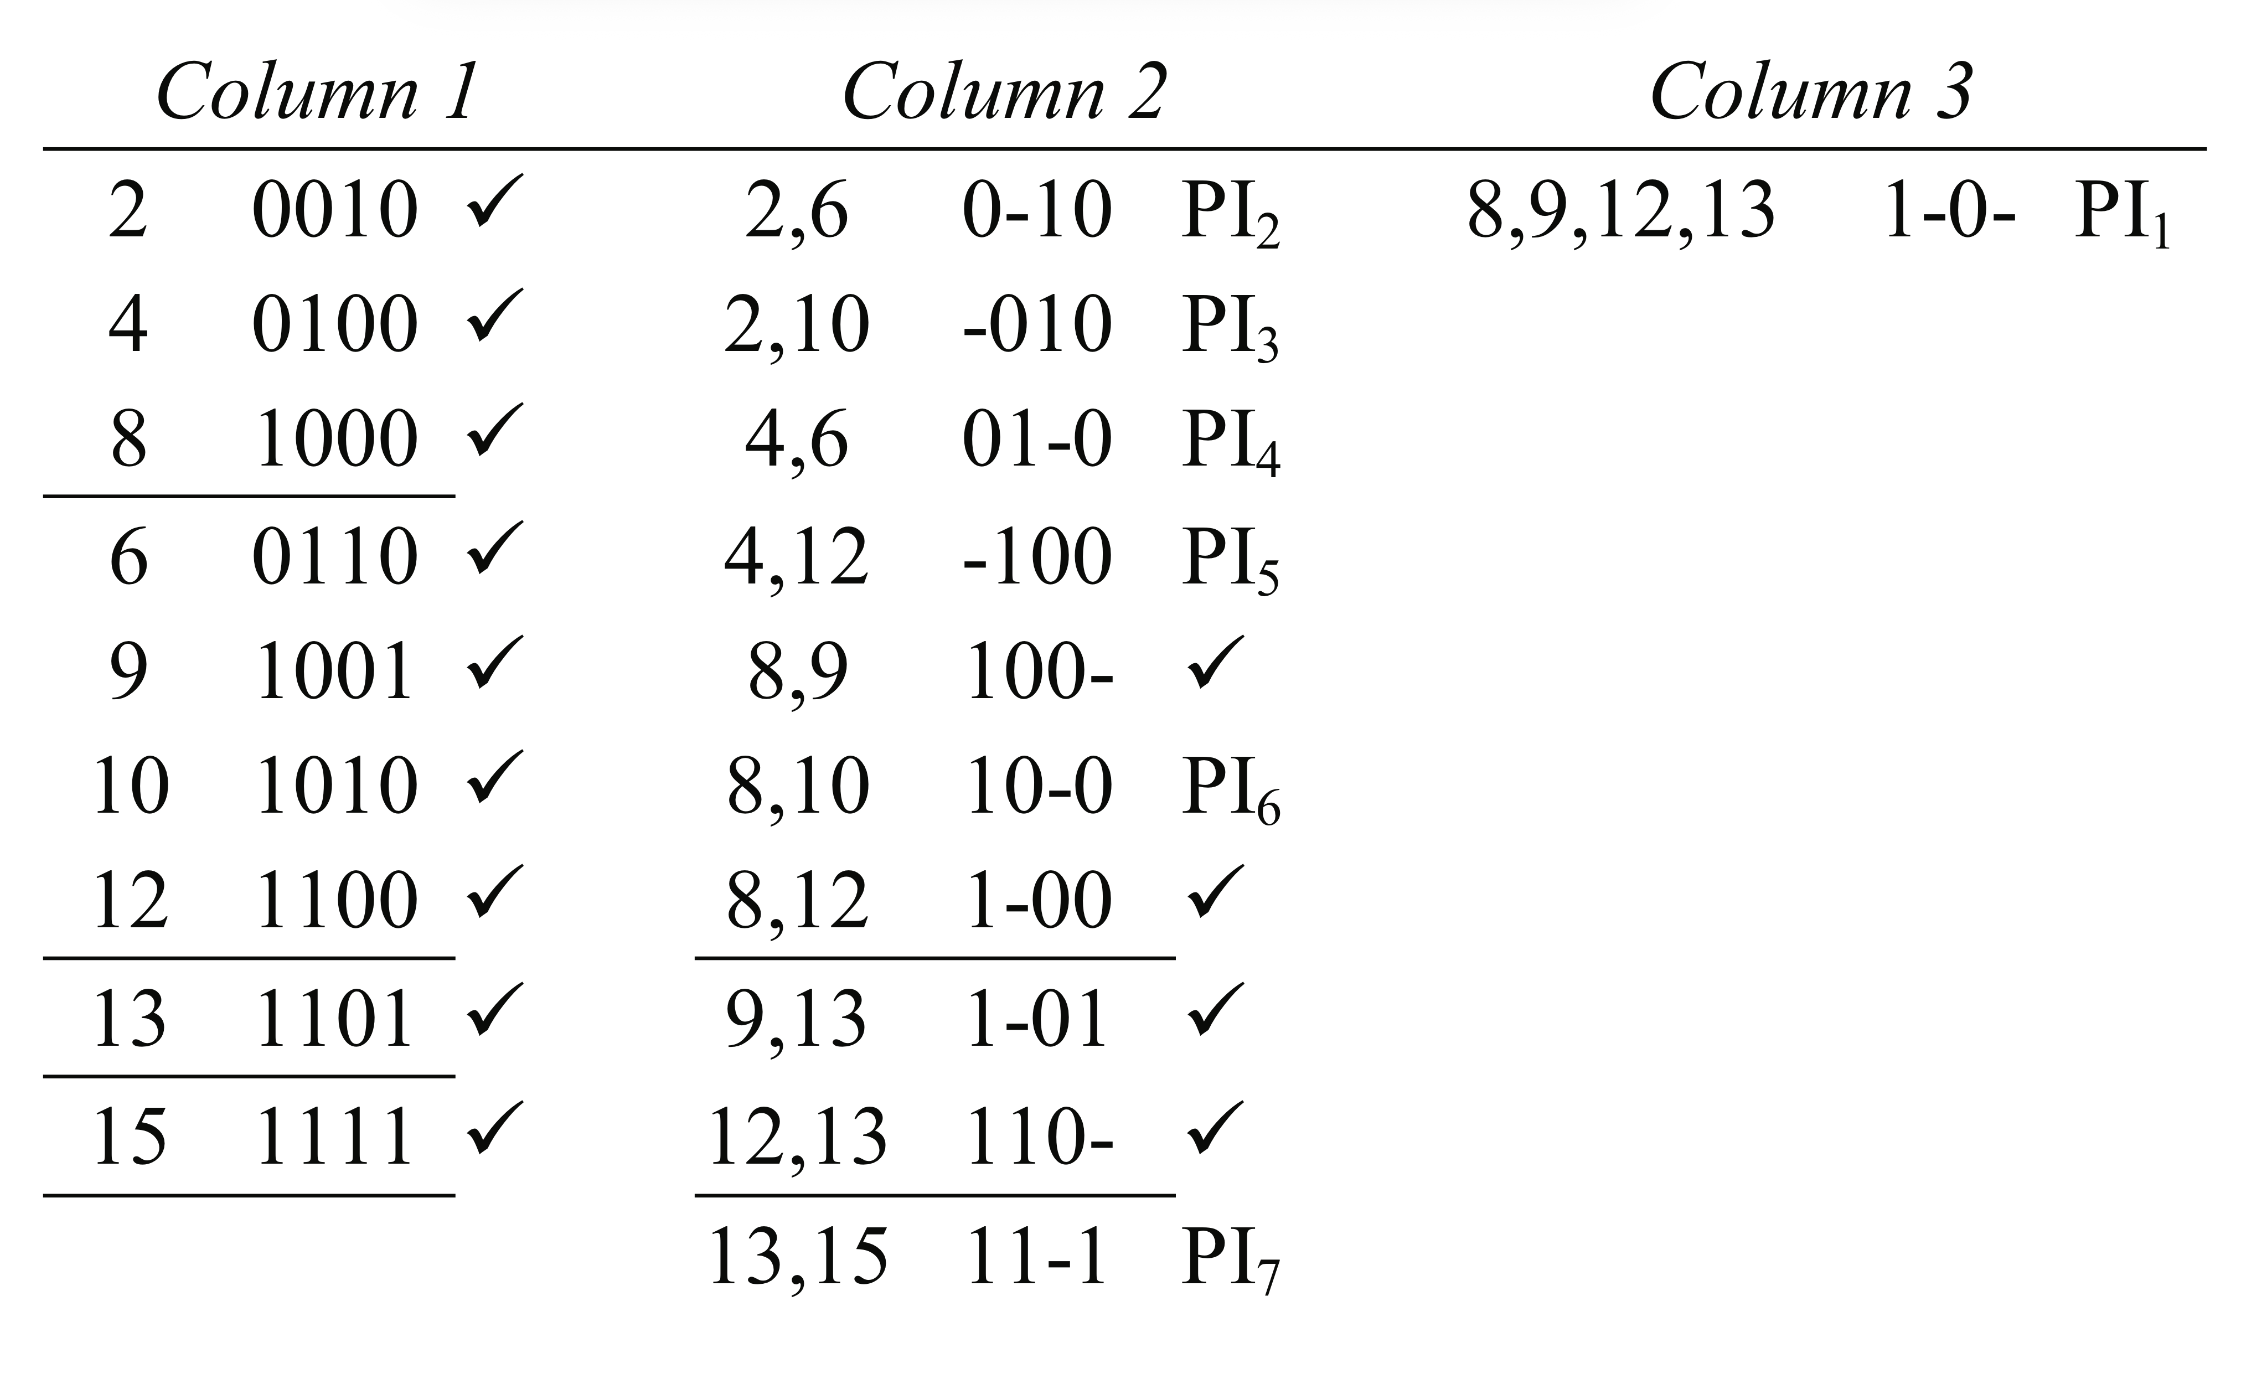
\includegraphics[width=0.5\textwidth]{quine_mccluskey}
  \end{figure}\\
  From this, we have the PI chart and then the reduced PI chart.
  \begin{figure}[h!]
    \centering
    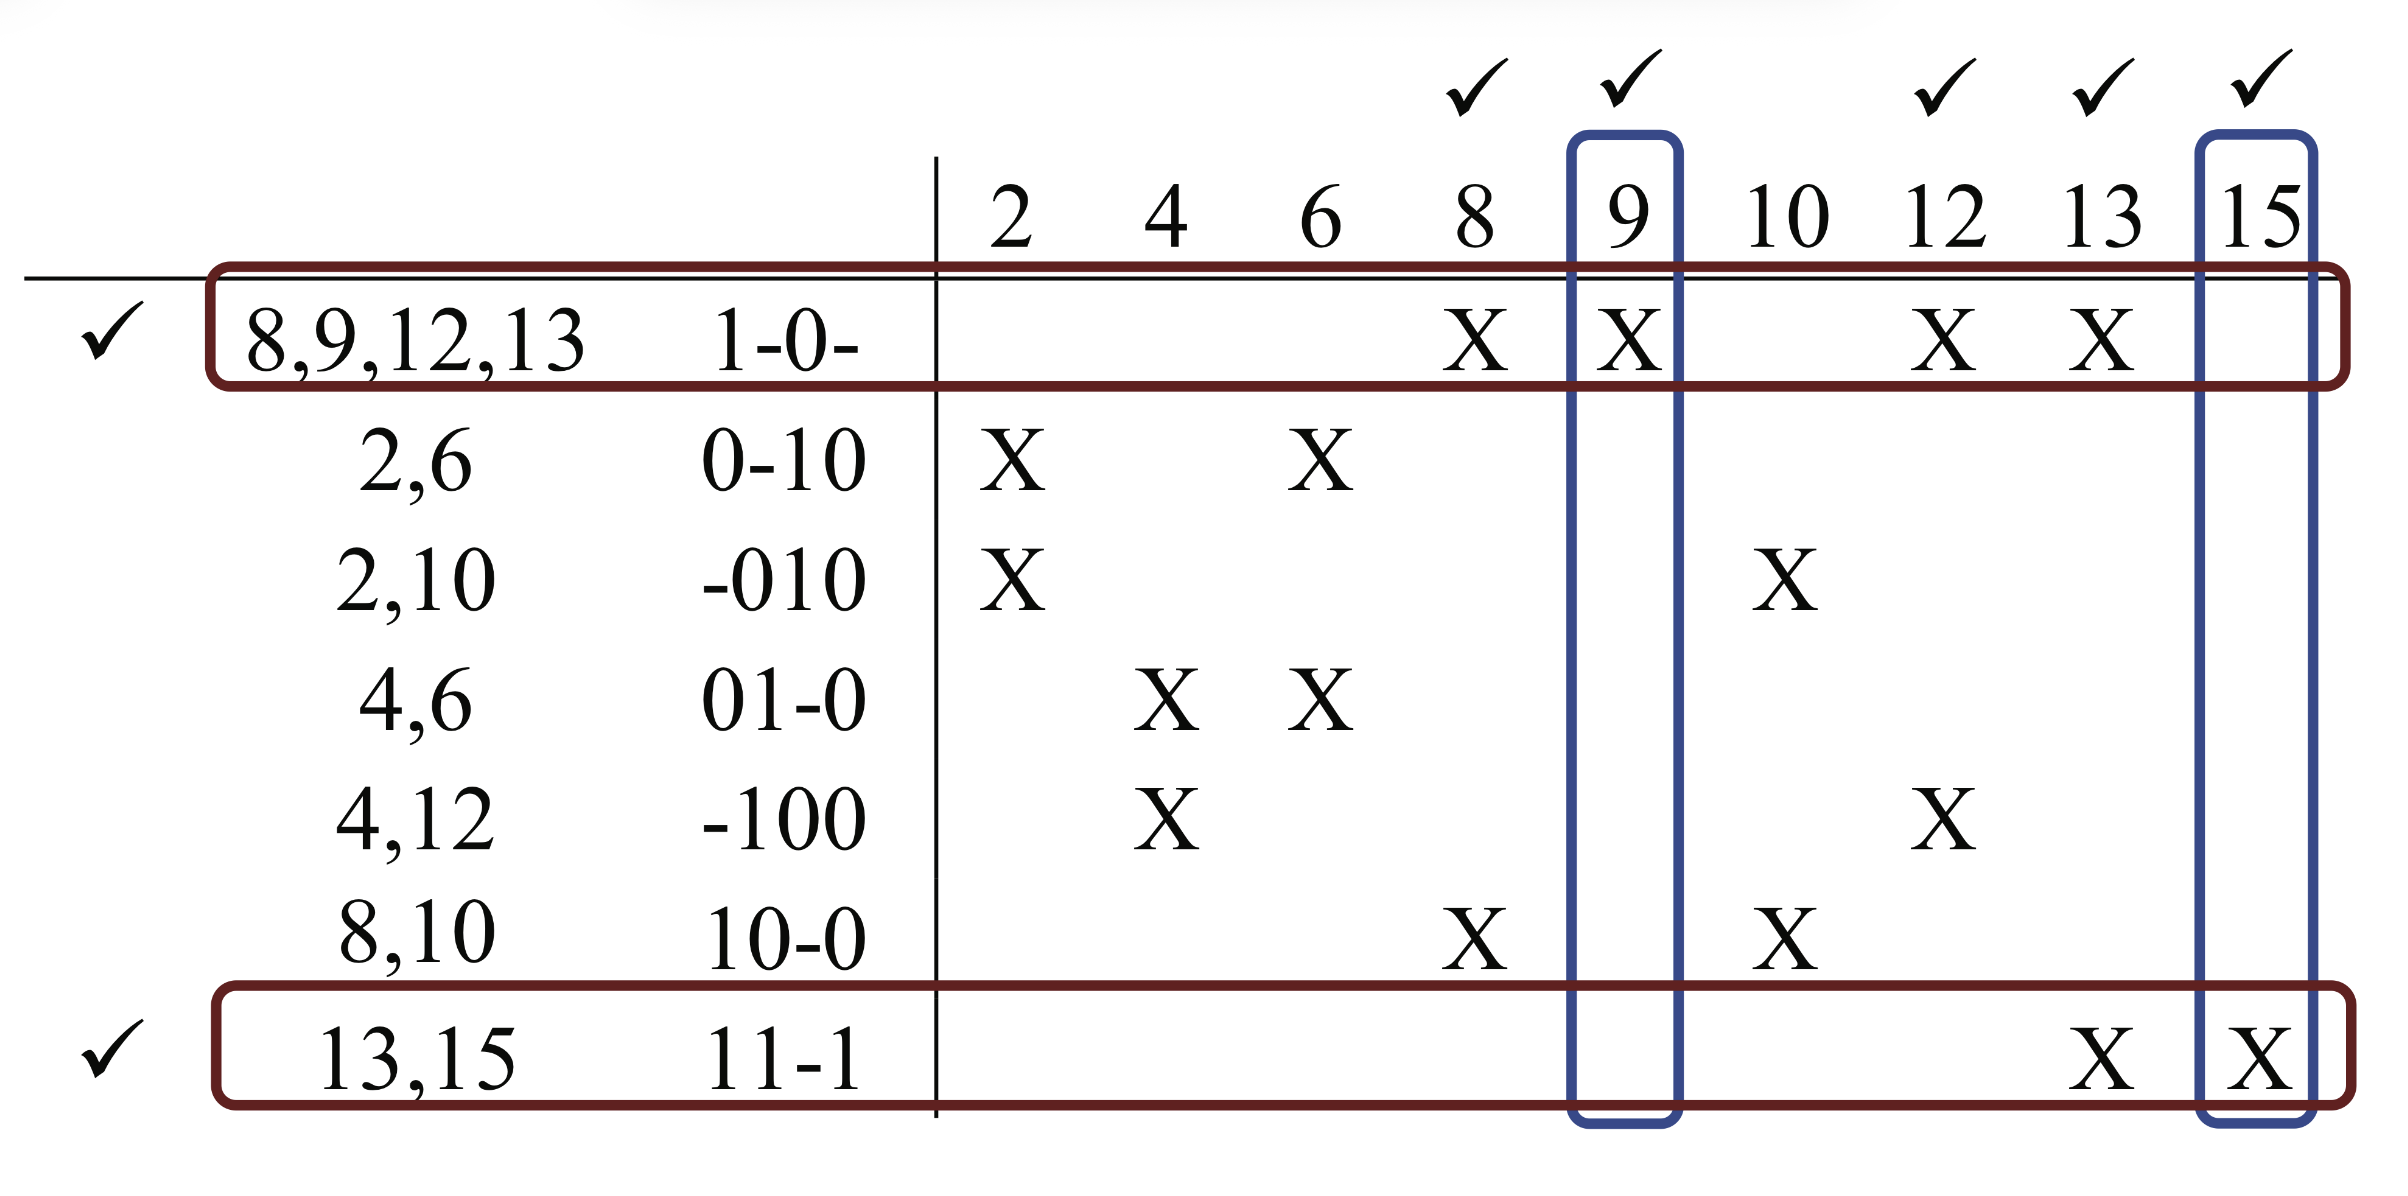
\includegraphics[width=0.4\textwidth]{quine_pi}
    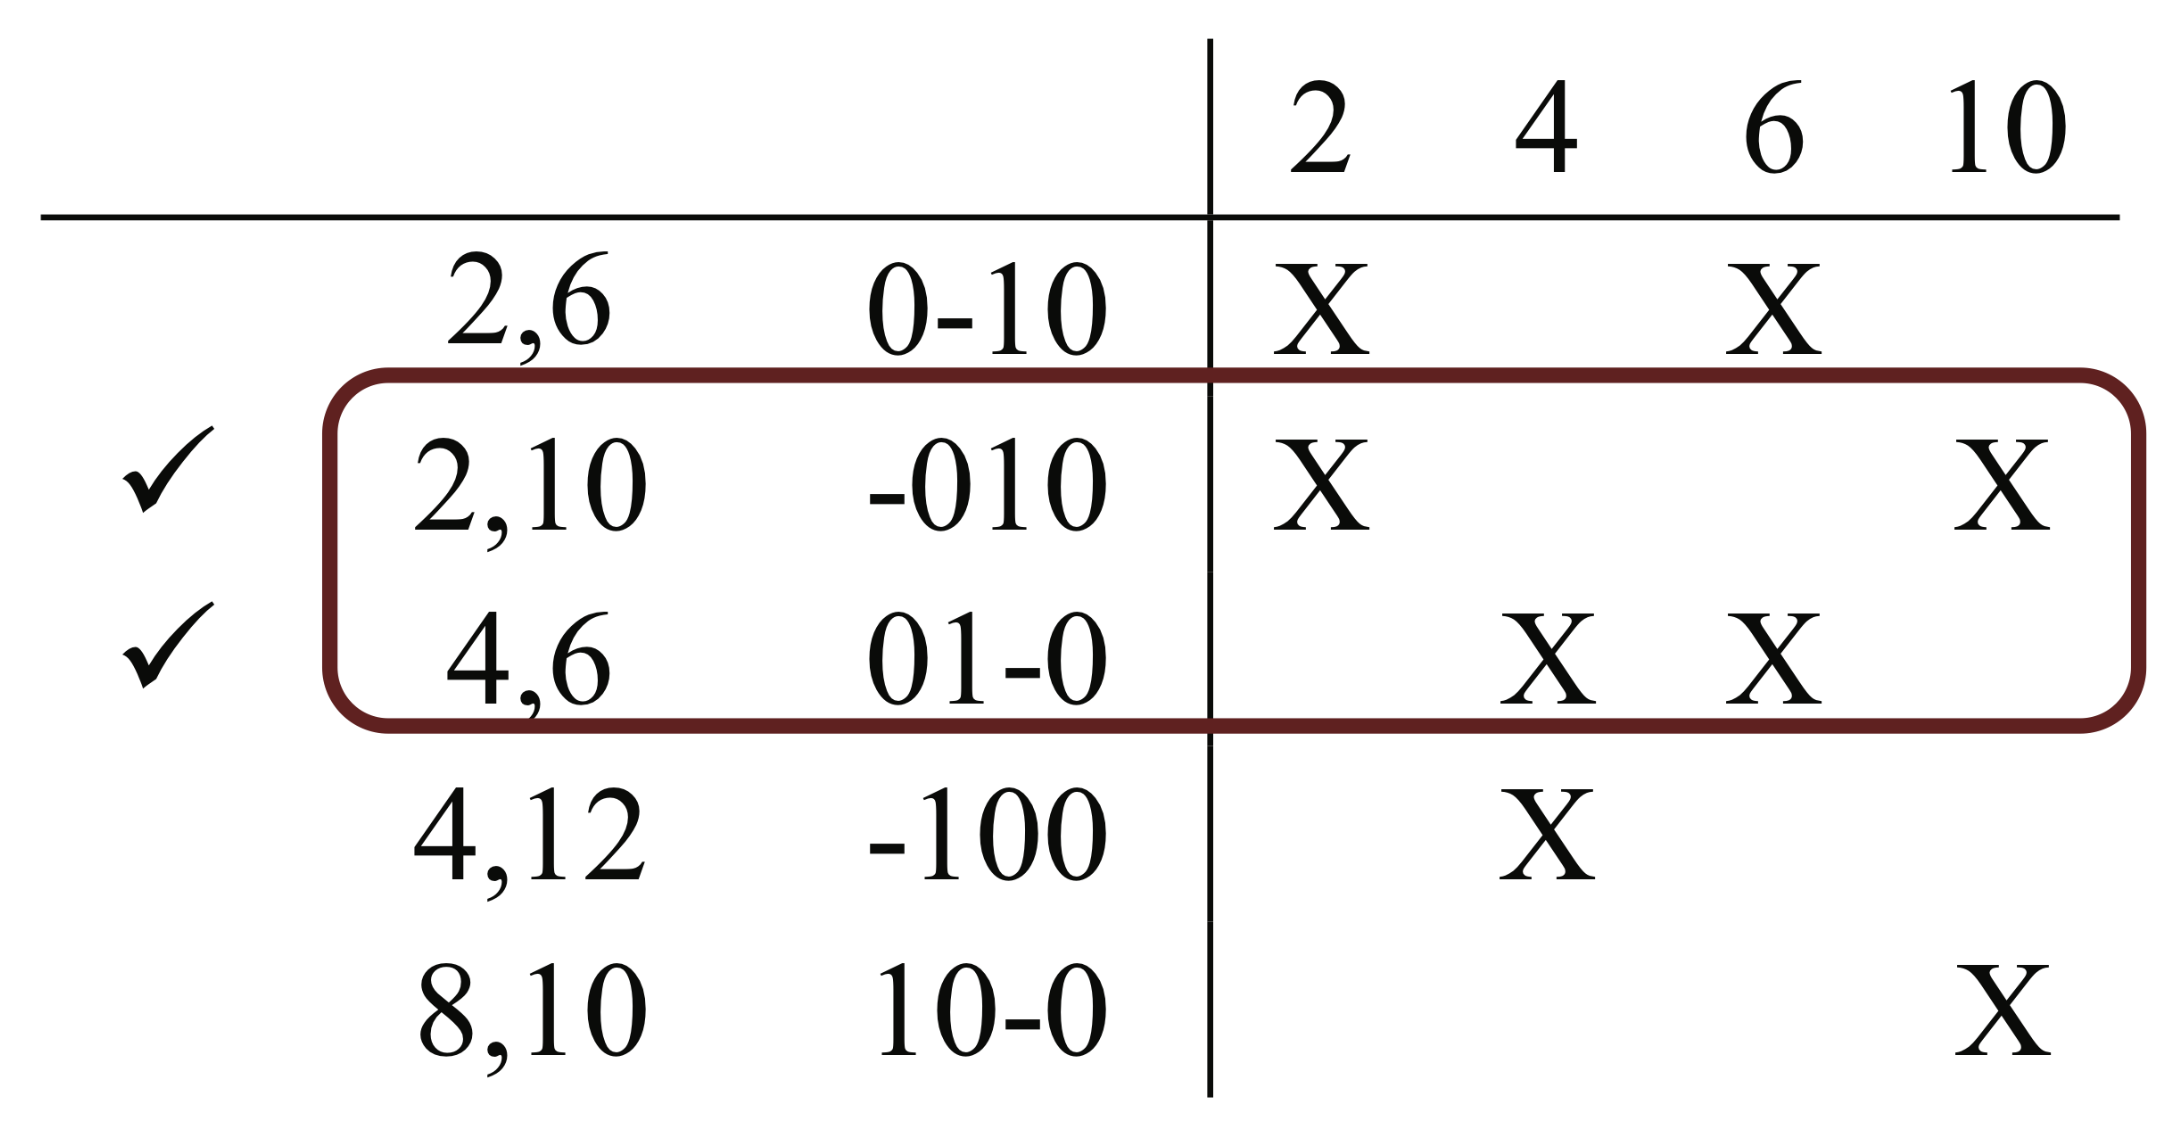
\includegraphics[width=0.3\textwidth]{quine_reducedpi}
  \end{figure}
  As such, we have the minimal SOP expression
  \[F=A\cdot C'+A\cdot B\cdot D+B'\cdot C\cdot D+A'\cdot B\cdot D'.\] 
\end{example}
This technique guarantees to produce a minimal standard form, and can be
applied to functions on many variables. However, it is highly tedious and more
suited for automation.


\subsection{Logic Circuits}
A logic circuit is composed of logic gates, represented as shown. We call the number of inputs of a gate the \textbf{fan-in}. Gates can have a fan-in more than 2.
\begin{figure}[h!]
  \centering
  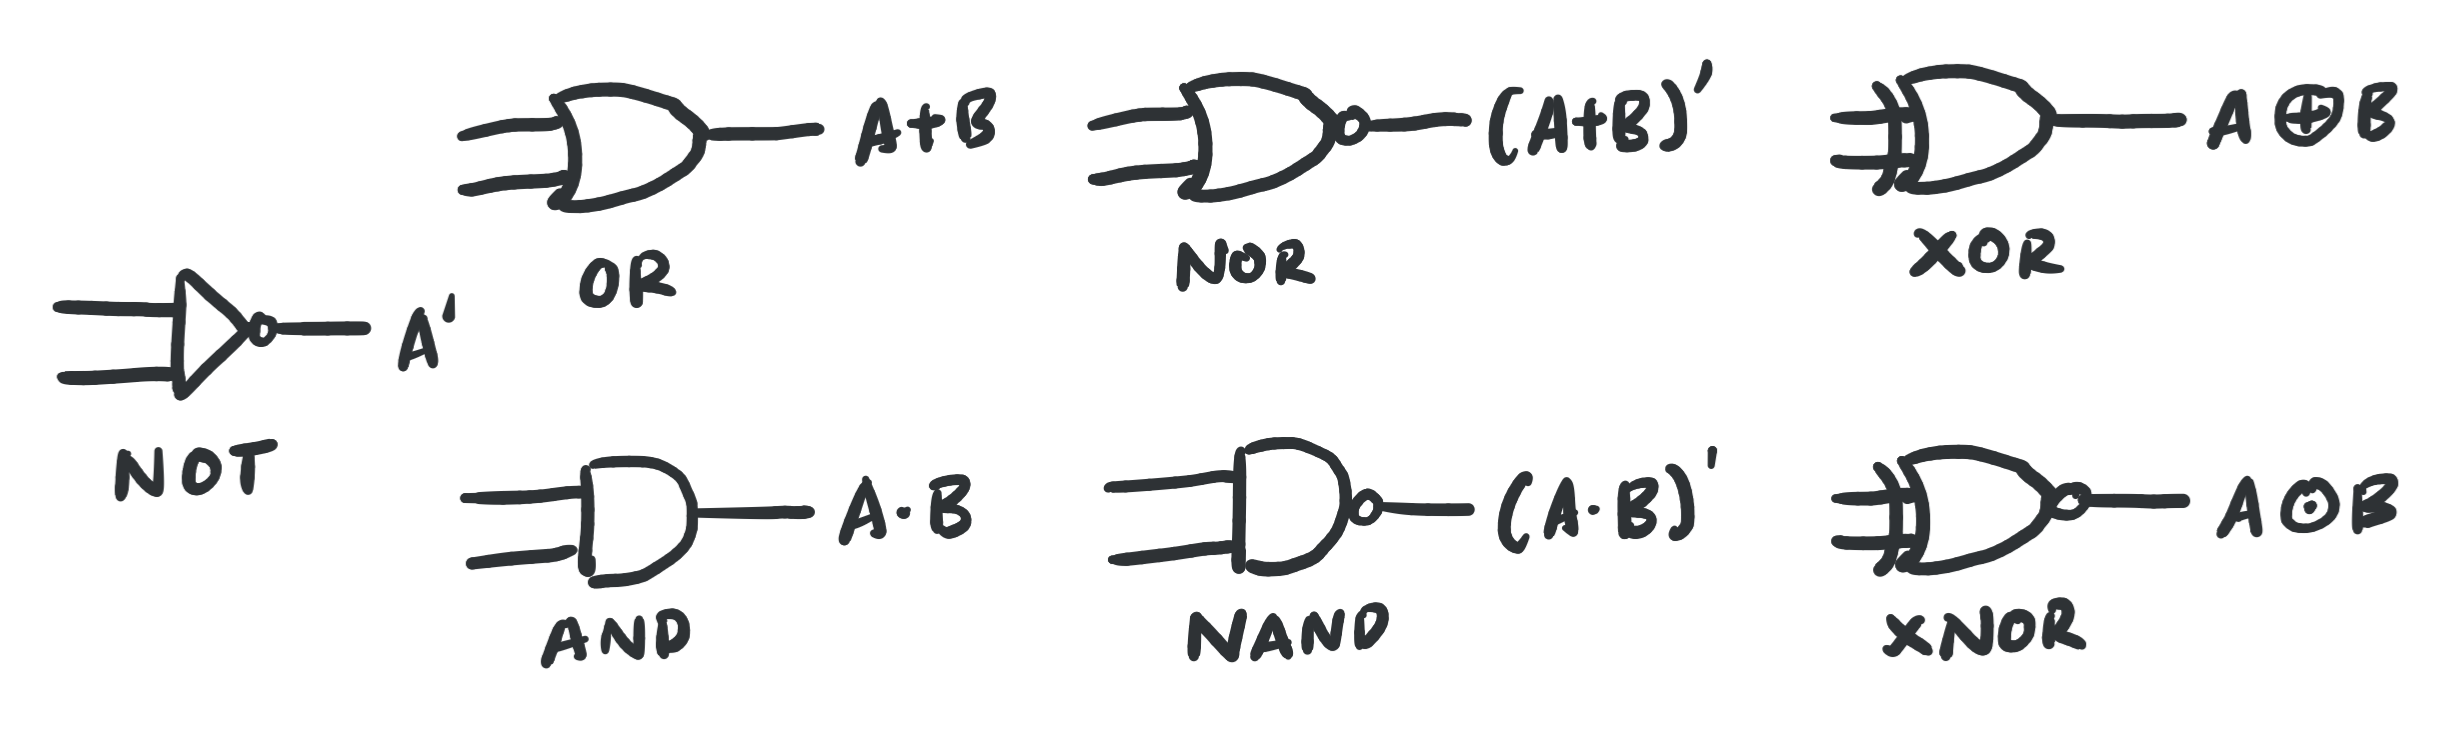
\includegraphics[width=0.5\textwidth]{logicGates.png}
\end{figure}
\begin{remark}
  By De Morgan's laws, we have the NAND $\equiv$ Negative-OR gate, and NOR $\equiv$ Negative-AND.
\end{remark}
Given a boolean expression, we may implement it as a logic circuit.
Additionally, given a logic circuit, we may obtain its logic expression.
We call the set $\left\{ AND, OR, NOT \right\} $ a \textbf{complete set of logic}. It is
sufficient for building any boolean function.
\begin{definition}[Universal Gates]
  A \textbf{Universal Gate} is a gate that itself is a complete set of logic. We may
  prove a specified gate is a universal gate by implementing a complete set of
  logic with the gate.
\end{definition}
\begin{example}[NAND]
  NAND is a universal gate.
  \begin{figure}[h!]
    \centering
    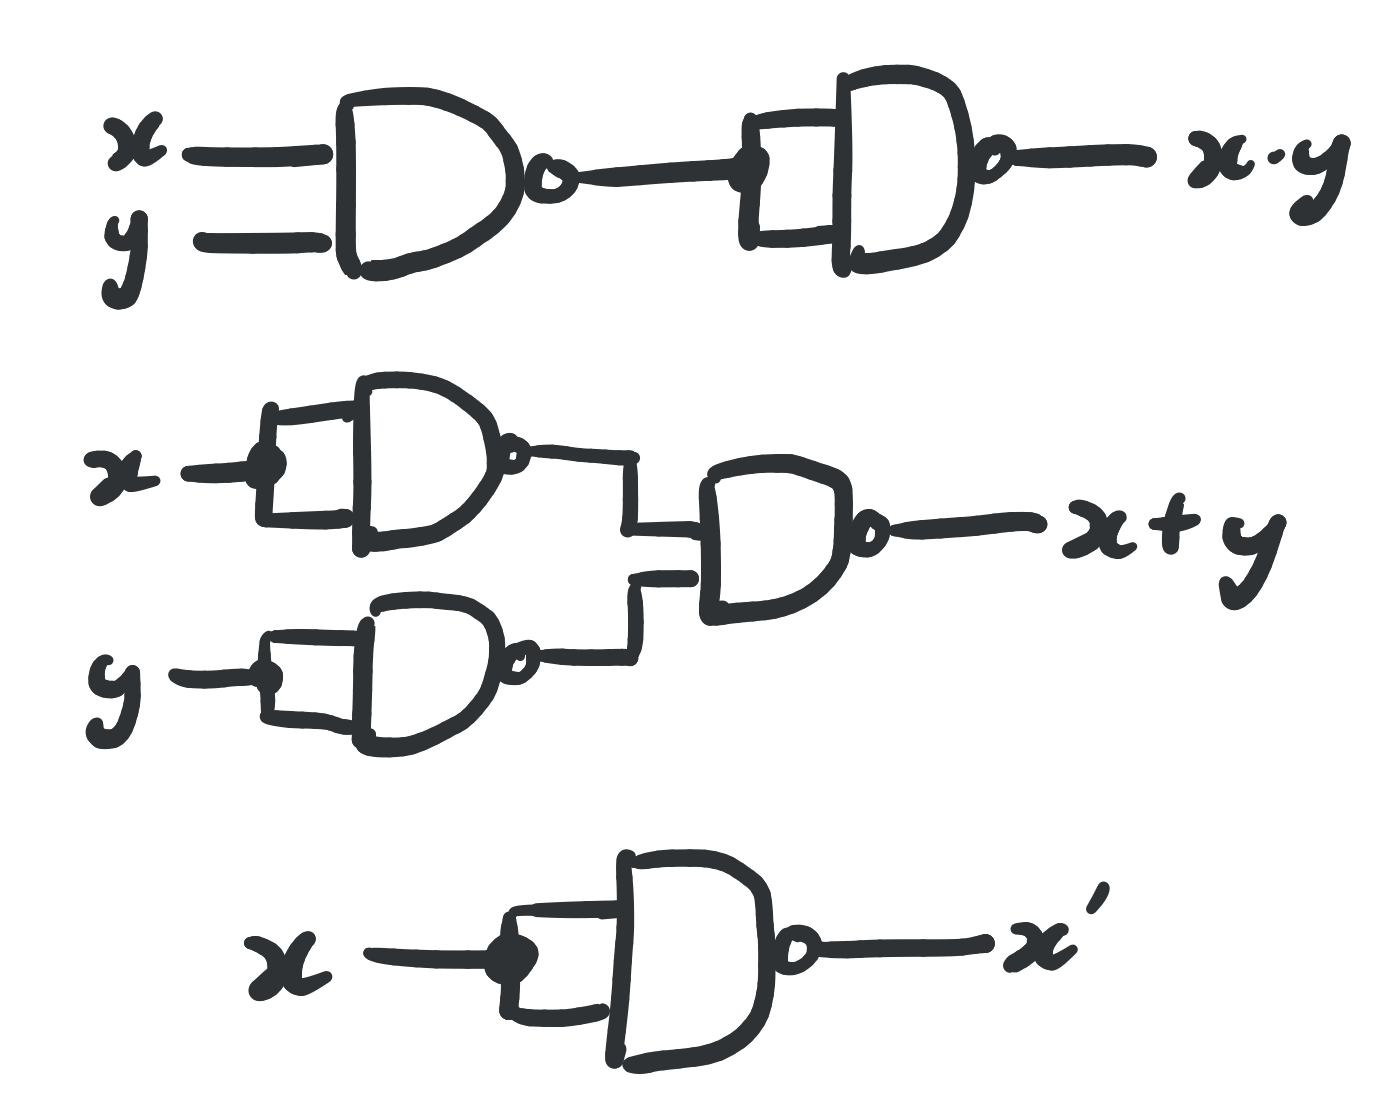
\includegraphics[width=0.25\textwidth]{nandUniversal}
  \end{figure}
\end{example}
\begin{example}[NOR]
  NOR is a universal gate.
  \begin{figure}[h!]
    \centering
    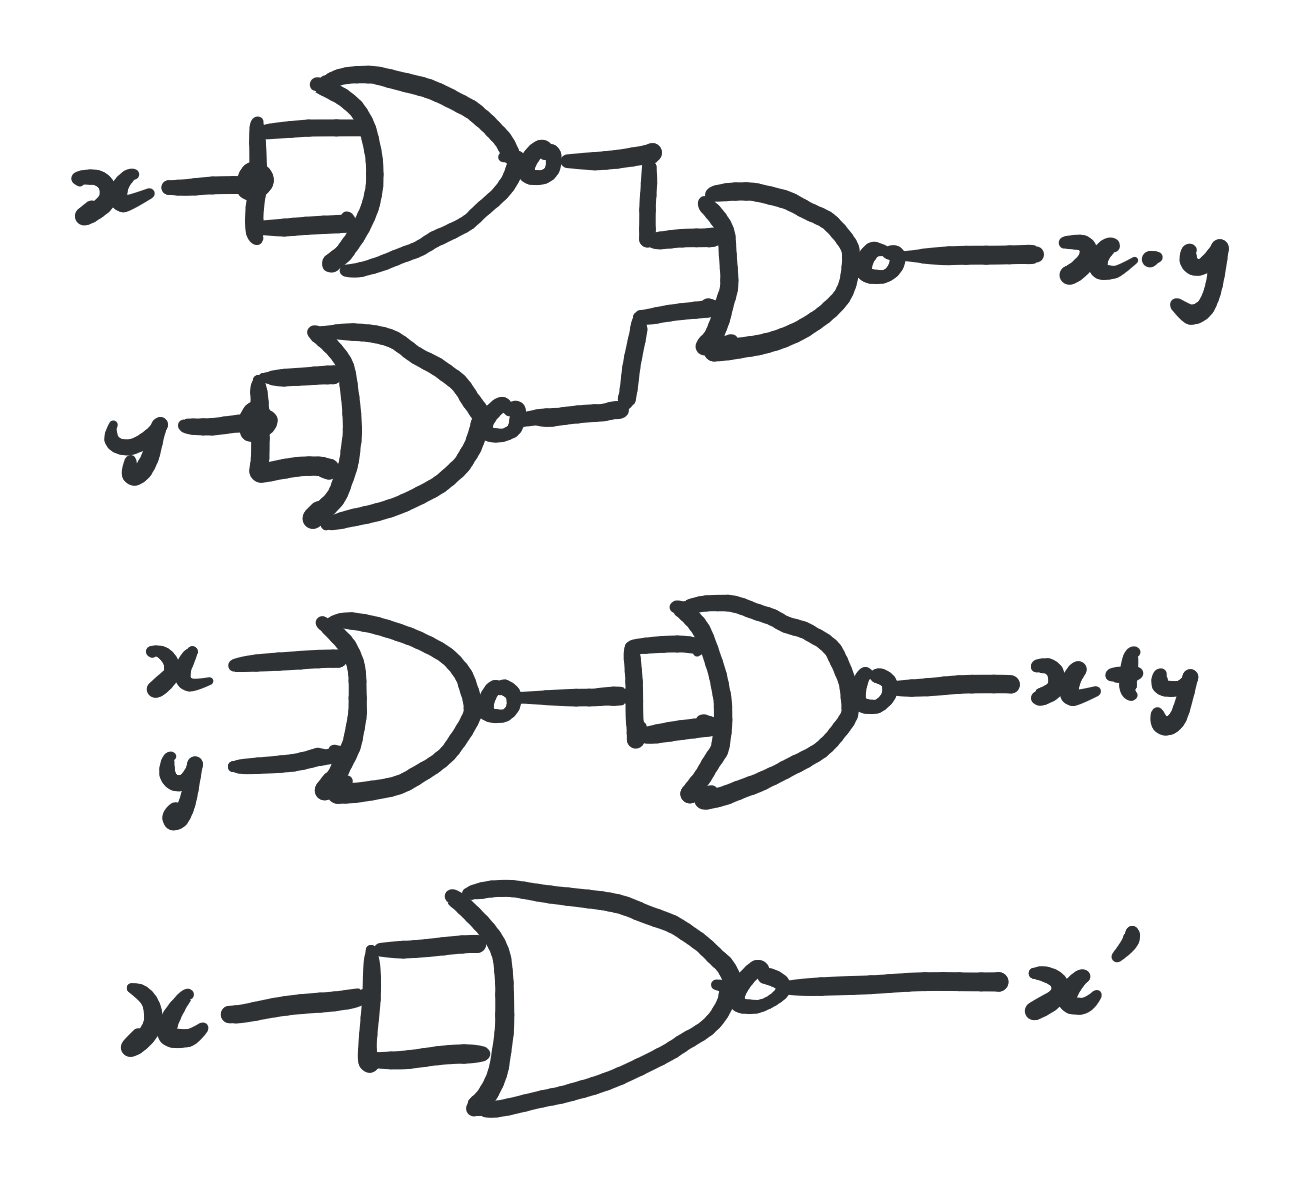
\includegraphics[width=0.25\textwidth]{norUniversal}
  \end{figure}
\end{example}
We may implement a given a SOP expression using a 2-level AND-OR circuit or a
2-level NAND circuit.
\begin{proof}
  With a SOP expression $F=A_0\cdot A_1 \cdot\ldots \cdot A_{n}+\cdots+Z_0\cdot
  Z_1\cdot\ldots\cdot Z_{n}$, we obtain each product term with AND gates for
  each product term, and obtain the final expression with a single OR gate.  By
  negating the output of each AND gate, and then negating the input to the OR
  gate, we obtain a 2-level circuit of NAND gates.\qed
\end{proof}\\
Similarly, we may implement a given a POS expression using a 2-level OR-AND
circuit or a 2-level NOR circuit.

\subsubsection{Propagation Delay}
\begin{definition}[Propagation Delay]
  The \textbf{gate delay} or \textbf{propagation delay} of a given gate is the
  average transition time taken for the output signal of the gate to change in
  response to changes in the input signals:
  \[t_{PD}=\left( t_{PHL} +t_{PLH}\right)/2 ,\] 
  where $t_{PHL}$ is the propagation delay time when the output changes from
  high to low, and $t_{PLH}$ that when the output changes from low to high.
\end{definition}
In general, given an $n$-input logic gate with delay $T$ and its inputs stable
at times $t_1,t_2,\ldots,t_{n}$, the earliest time in which the output is
stable is $max\left\{ t_1,t_2,\ldots,t_{n} \right\} +T$.

\begin{definition}[Circuit Delay]
  The \textbf{circuit delay} is the ``propagation of the entire circuit'', the
  longest time it takes for the input signals to propagate to the outputs.
\end{definition}
\begin{example}[Circuit Delay]
  Given a circuit, we can calculate the circuit delay by propagating the inputs
  forward past each logic gate or component to obtain the final delay.
  \begin{figure}[h!]
    \centering
    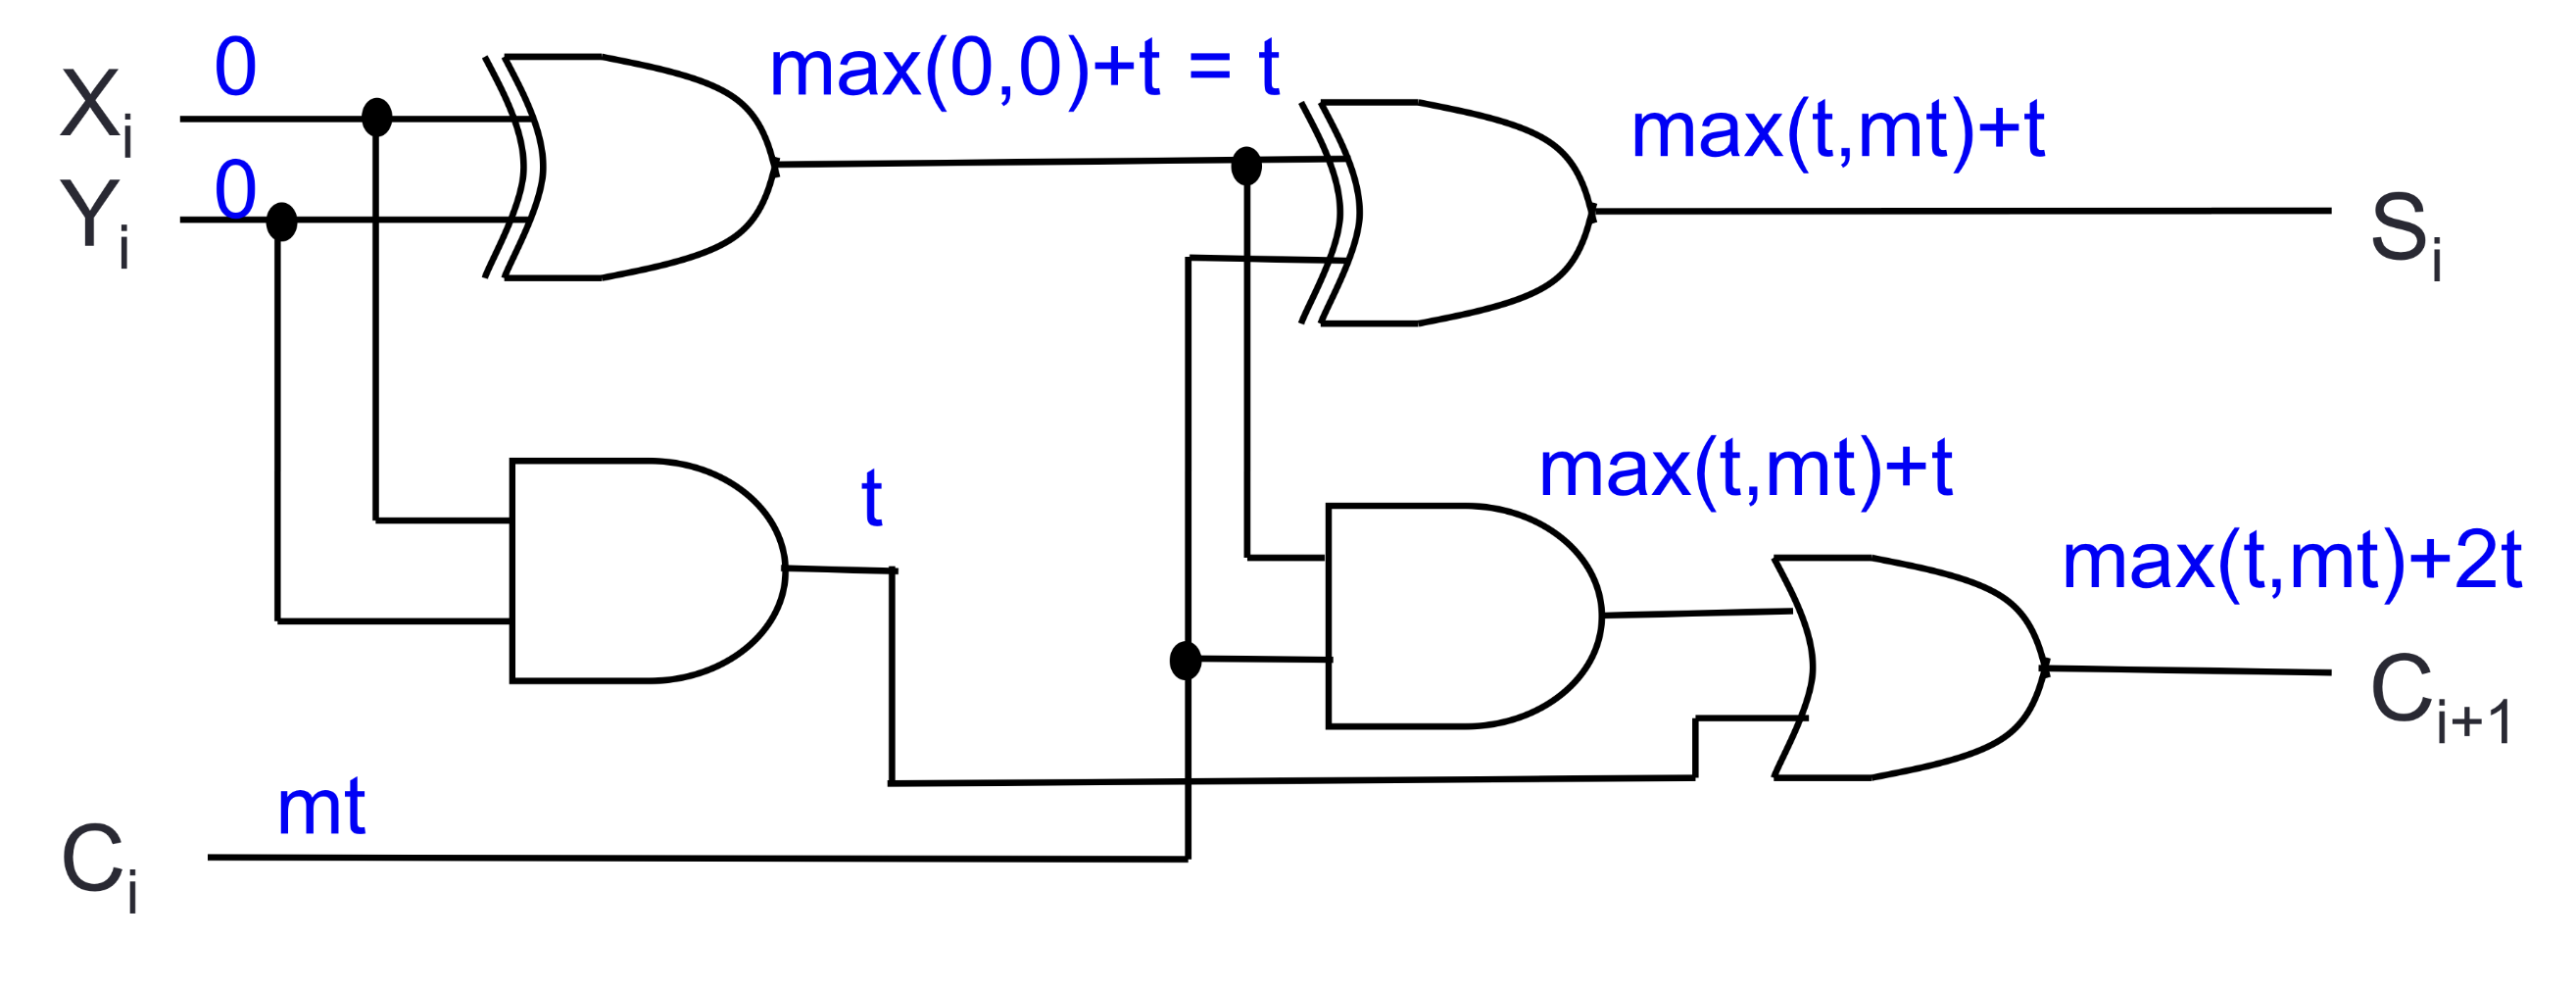
\includegraphics[width=0.5\textwidth]{circuit_delay}
  \end{figure}
\end{example}

\subsubsection{Alternative Logic Circuits}
\paragraph{Integrated Circuit}
\begin{definition}[Integrated Circuit]
  An \textbf{Integrated Circuit }(IC), also known as a chip or microchip, is a
  semiconductor device in which transistors, capacitors and resistors are
  fabricated.
\end{definition}
ICs can be categorised according to the number of components they contain,
\begin{itemize}
  \item \textit{Small Scale Integration}: Up to 100 electronic components
  \item \textit{Medium-Scale Integration}: From 100 to 3,000 electronic components
  \item \textit{Large-Scale Integration}: From 3,000 to 100,000 electronic components
  \item \textit{Very Large-Scale Integration}: From 100,000 to 1,000,000 electronic components
  \item \textit{Ultra Large-Scale Integration}: More than 1,000,000 electronic components
\end{itemize}
or according to its capabilities and limitations, into different logic families:
\begin{itemize}
  \item \textit{Transistor-Transistor Logic}: Uses bipolar junction transistors
  \item \textit{Complementary Metal-Oxide Semiconductor}: Uses metal-oxide
    semiconductor field effect transistors, consumes less power and has higher
    packing density, but is very sensitive to static electricity
  \item \textit{Emitter-Coupled Logic}: Uses bipolar circuit technology,
    designed for very high speed operations, but has high power consumption.
  \item among many others…
\end{itemize}

\begin{example}[TTL]
  The Transistor-Transistor Logic family is the largest, consisting various
  versions: \textit{standard TTL, low-power TTL, Schottky TTl, low-power
  Schottky TTL, advanced Schottky TTL,} etc. These ICs are encoded by four- to
  five-digit part numbers, with a two-digit prefix (usually 54 or 74) followed
  by a two- or three-digit code for the gate. Between the prefix and the gate
  code is a letter code indicating the TTL version.
\end{example}

\paragraph{Programming Logic Array}
\begin{definition}[Programming Logic Array]
  A \textbf{Programming Logic Array }(PLA) is a programmable integrated circuit
  that implements SOP circuits with multiple outputs using a 2-level AND-OR
  circuit.
\end{definition}
\begin{figure}[h!]
  \centering
  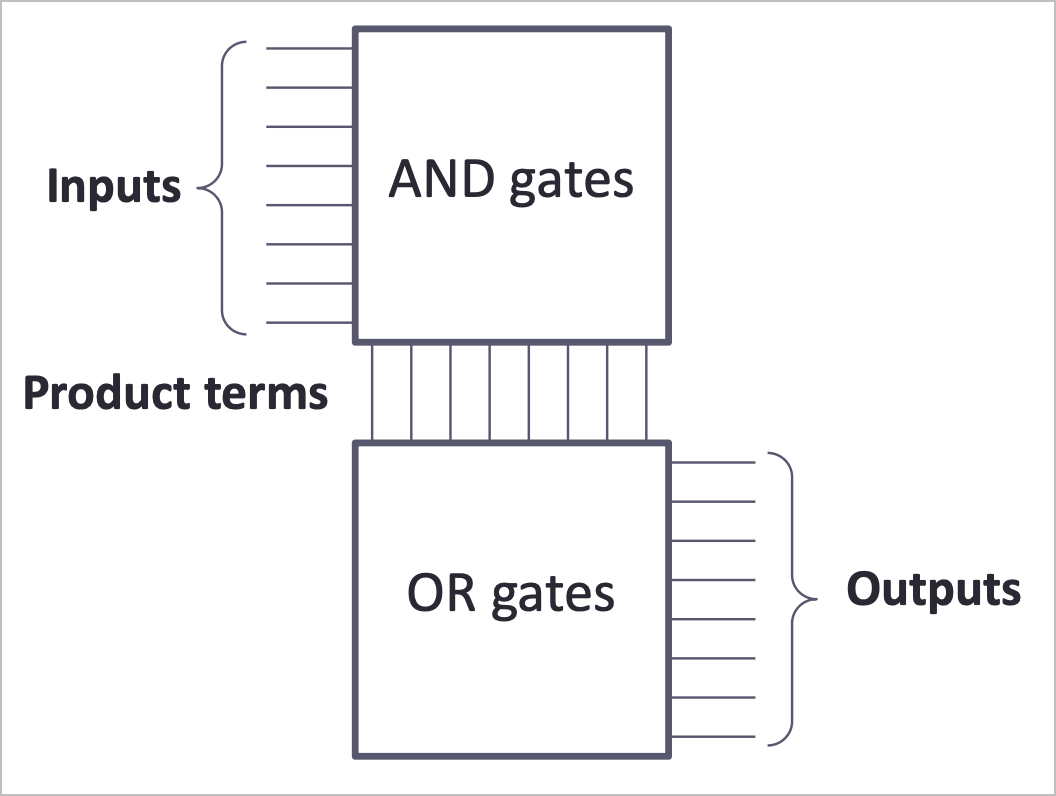
\includegraphics[width=0.3\textwidth]{PLA.png}
\end{figure}

\paragraph{Read Only Memory}
\begin{definition}[Read Only Memory]
  A \textbf{Read-Only Memory} is similar to PLA with a set of inputs
  (addresses) and a set of outputs, with a programmable mapping between inputs
  and outputs.
\end{definition}
A ROM is fully decoded and able to implement any mapping, in contrast to PLA
which may not have enough minterms.

\subsubsection{MSI Components}
In addition, we have various common medium-scale integration (MSI) components
that are used in circuit design, namely the \textit{decoders},
\textit{encoders}, \textit{demultiplexers}, and \textit{multiplexers}.

\paragraph{Decoders}
\begin{definition}[Decoders]
  A $n$-to-$m$-line, $n:m$, or $n\times m$ \textit{decoder}, converts binary
  information from $n$ input lines to $m\le 2^{n}$ output lines. Given an input
  of $k_{10}={\left( X_{n}X_{n-1}\cdots X_1 \right)}_2$, the decoder selects
  the $k$-th output line.
\end{definition}
\begin{remark}
  Each output is the minterm of all the variables, since every code uniquely
  identifies an output line to be selected.
\end{remark}
\begin{definition}[Enable]
  In these components, we may have an \textit{enable control} sigal, such that
  the device is only activated when the enable $E=1$. We say that the device is
  one-enable.
  \begin{figure}[h!]
    \centering
    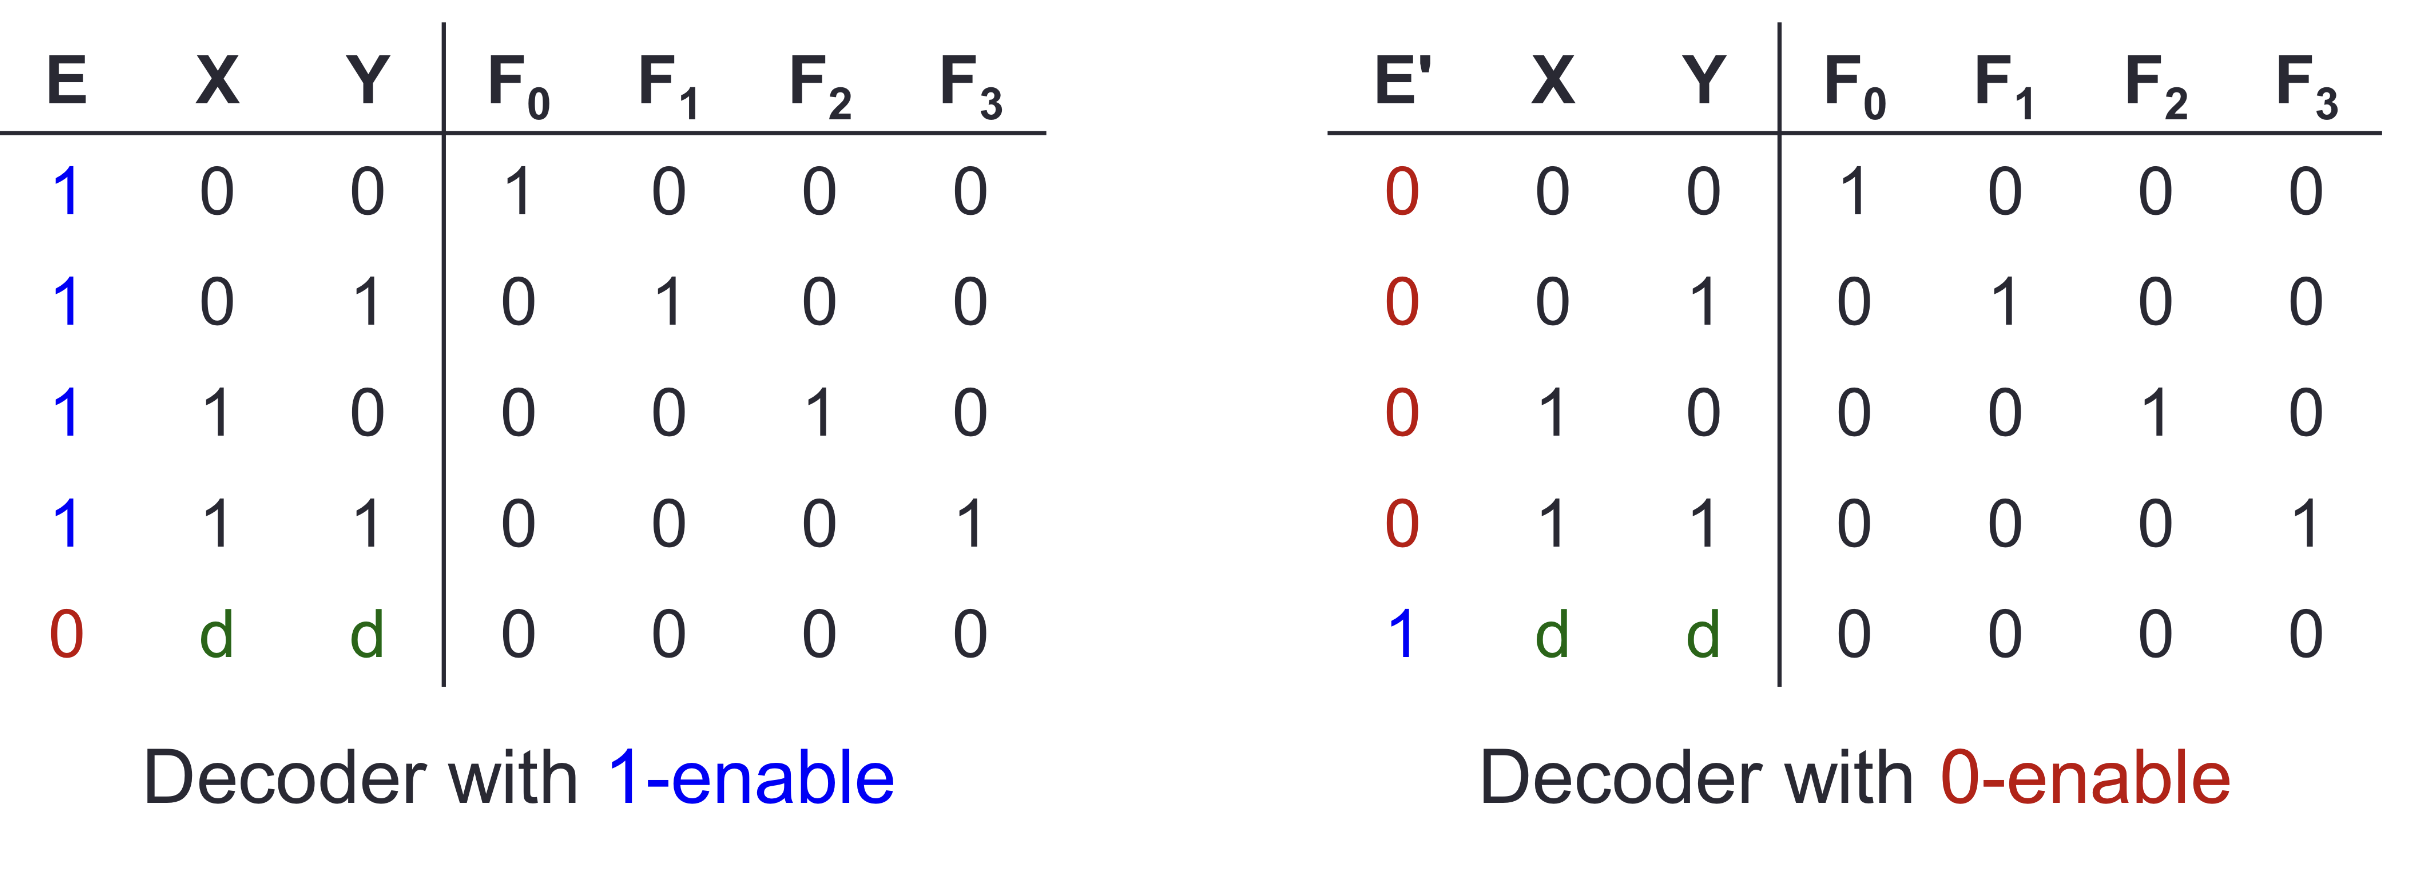
\includegraphics[width=0.5\textwidth]{decoder_enable}
  \end{figure}\\
  Enables may be implemented with an AND gate for each of the outputs.
\end{definition}
\begin{definition}[Active High/Low Outputs]
  A device has normal outputs if it has active high outputs, and negated
  outputs if it has active low outputs.
\end{definition}
\begin{remark}
  Most Standard MSI Decoders are zero-enabled, and have active-low outputs.
  \begin{example}[74138 $3:8$ Decoder]
    We illustrate the representations of a standard 74138 decoder, a
    zero-enabled, active-low output, $3:8$ decoder.
    \begin{figure}[h!]
      \centering
      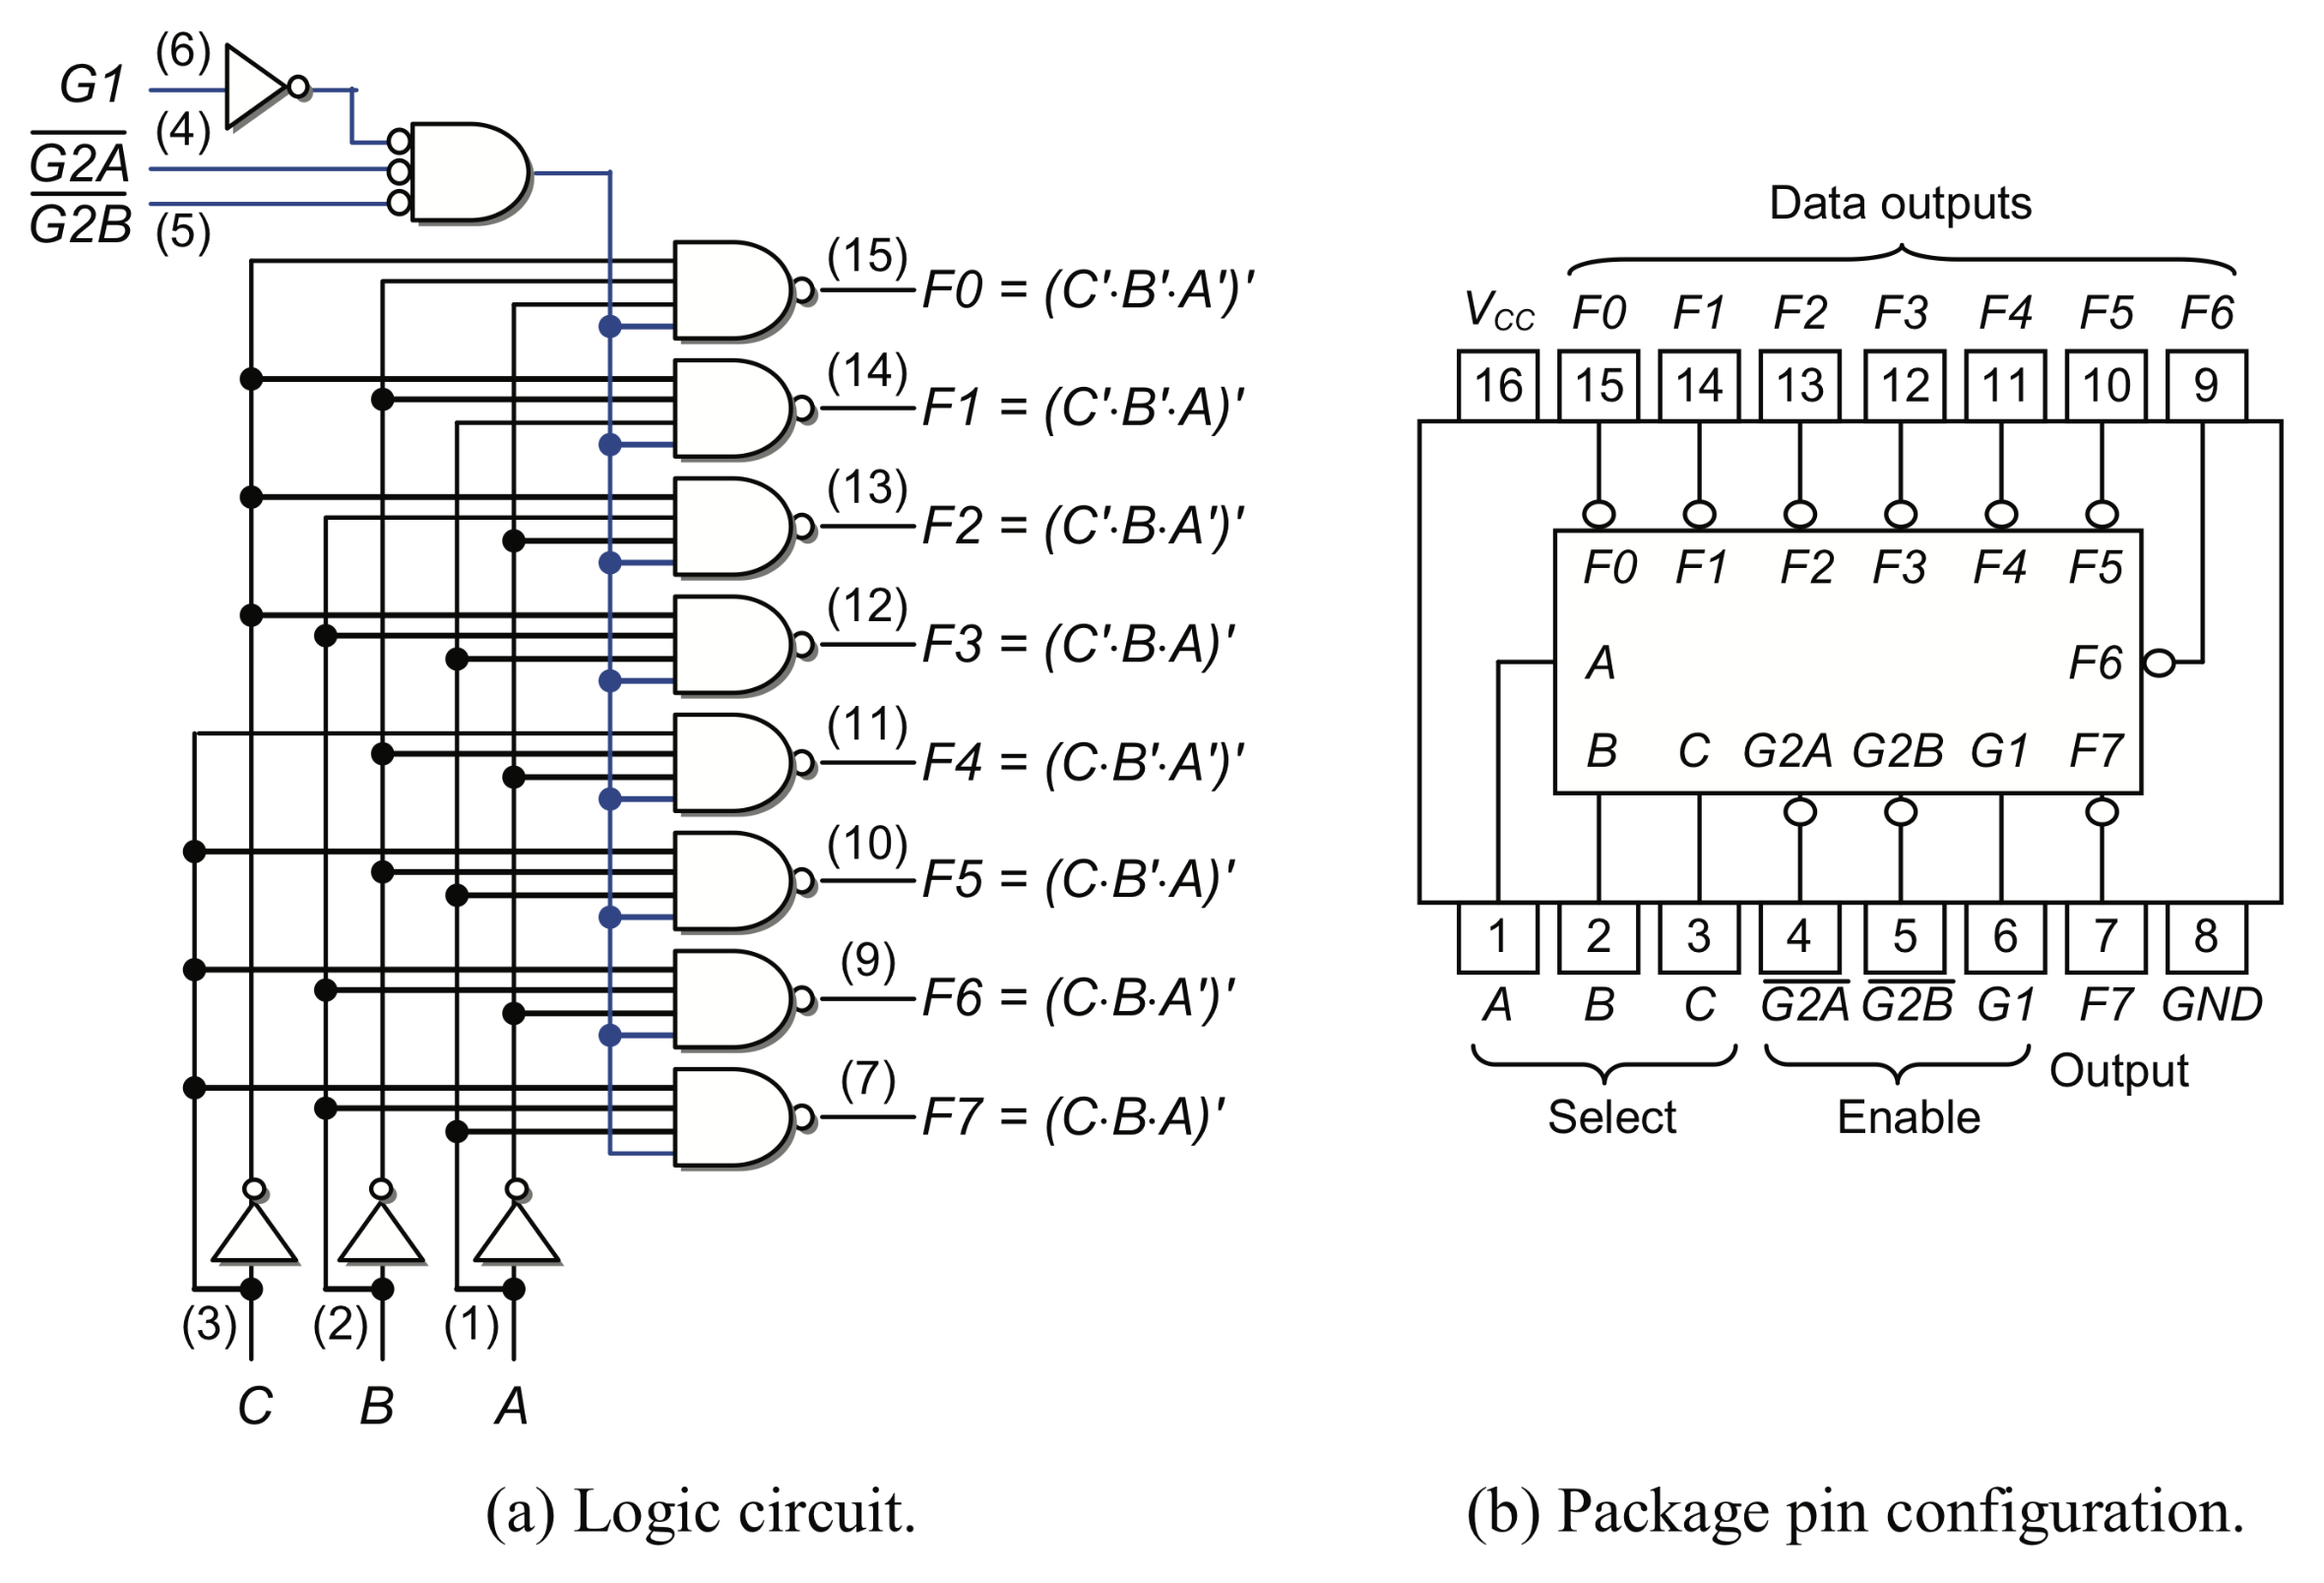
\includegraphics[width=0.5\textwidth]{decoder_74138}
      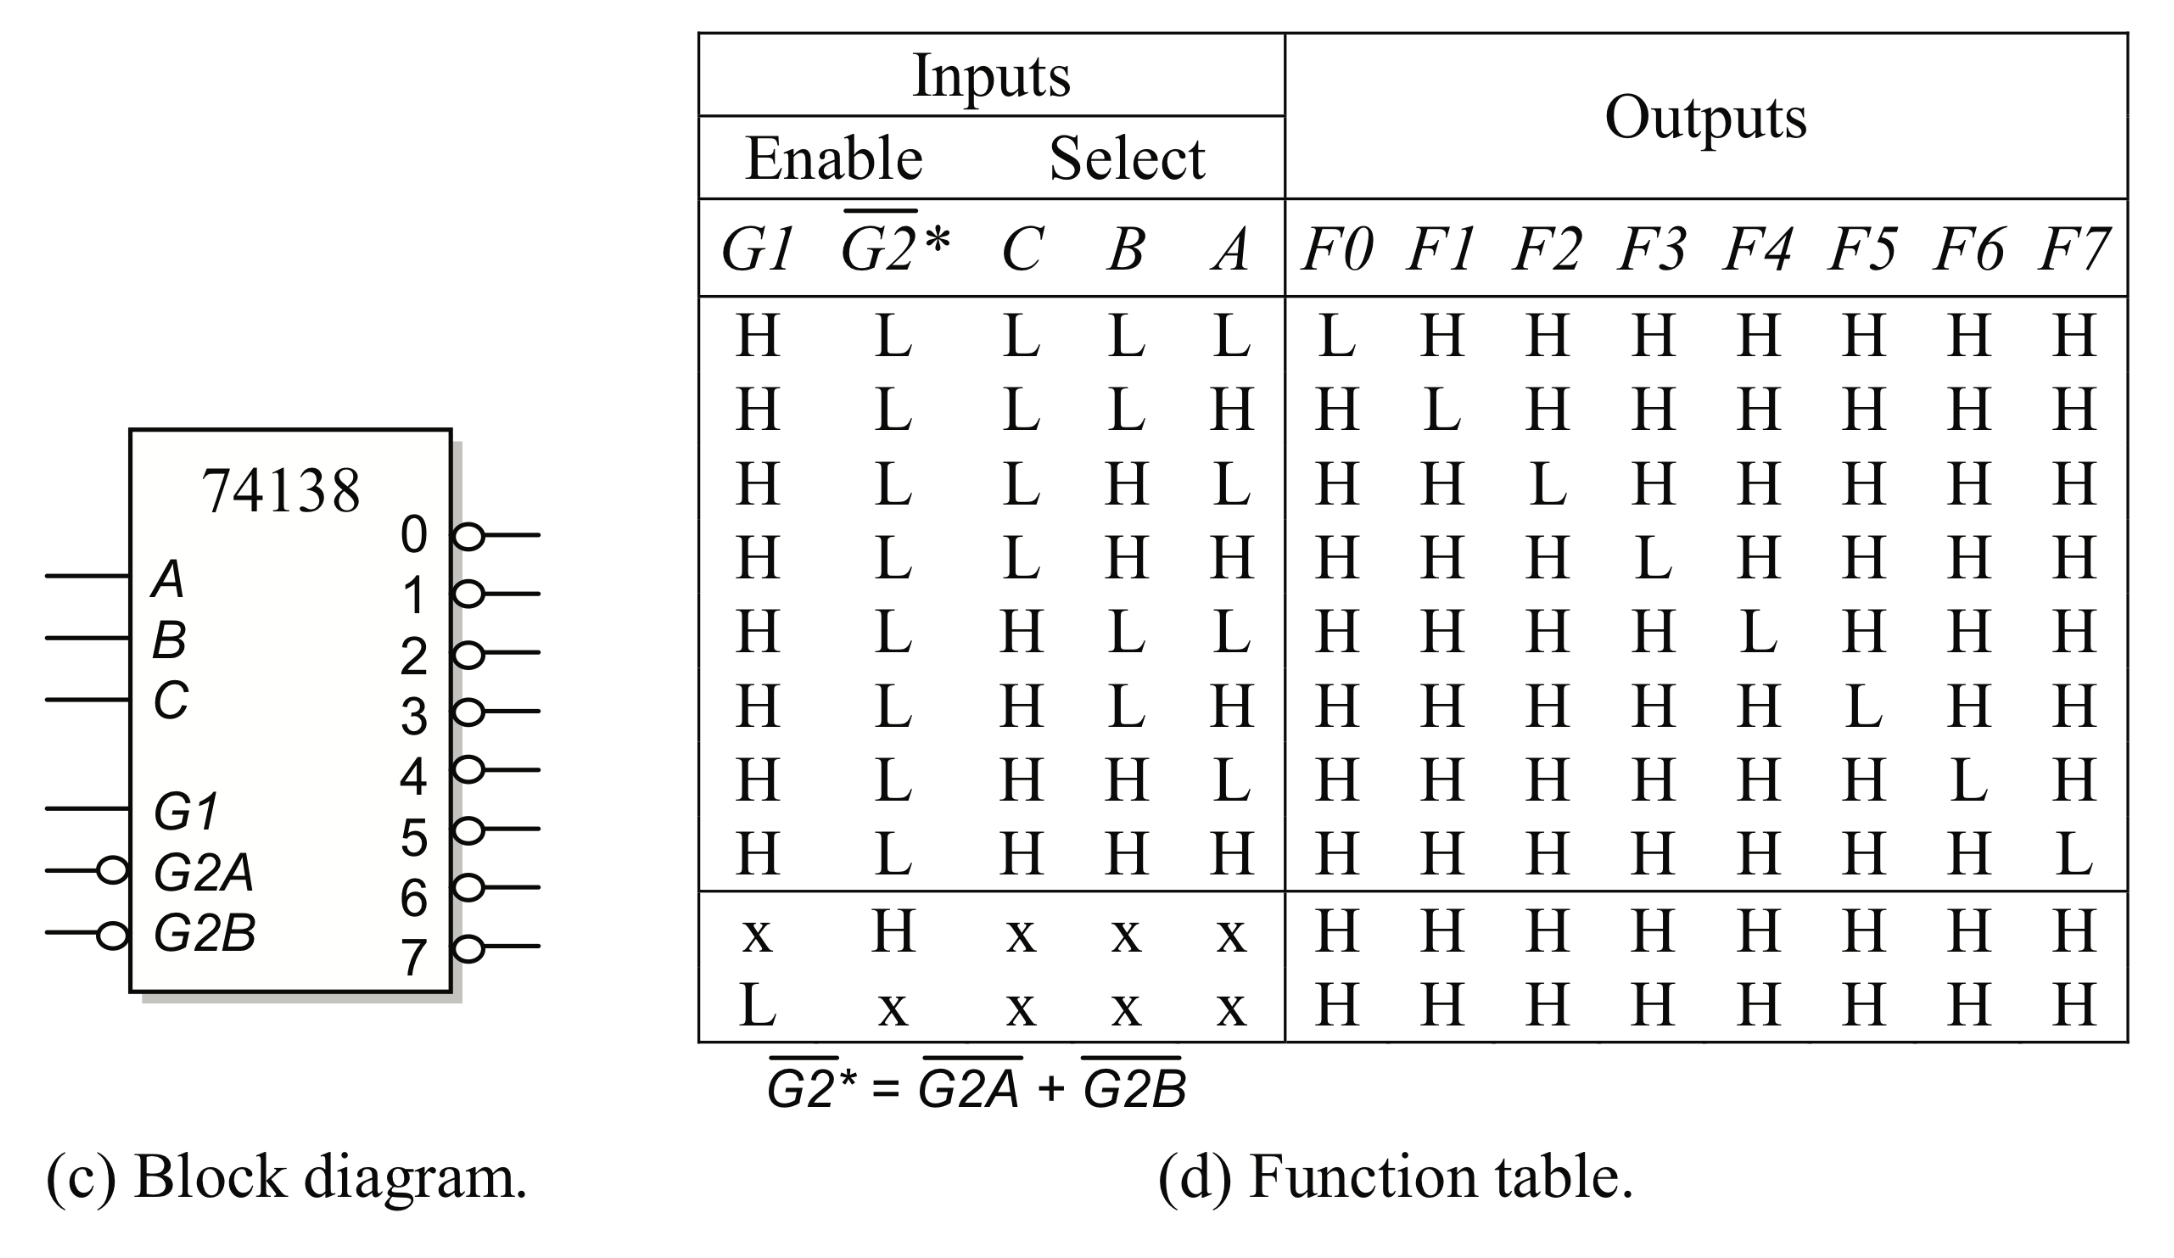
\includegraphics[width=0.4\textwidth]{decoder_74138_2}
    \end{figure}
  \end{example}
\end{remark}
Additionally, decoders can also be cascaded to construct larger decoders.
\begin{example}[$3:8$ Decoder]
  We can construct a $3:8$ decoder from two $2:4$ decoders with one-enable and
  an inverter.
  \begin{figure}[h!]
    \centering
    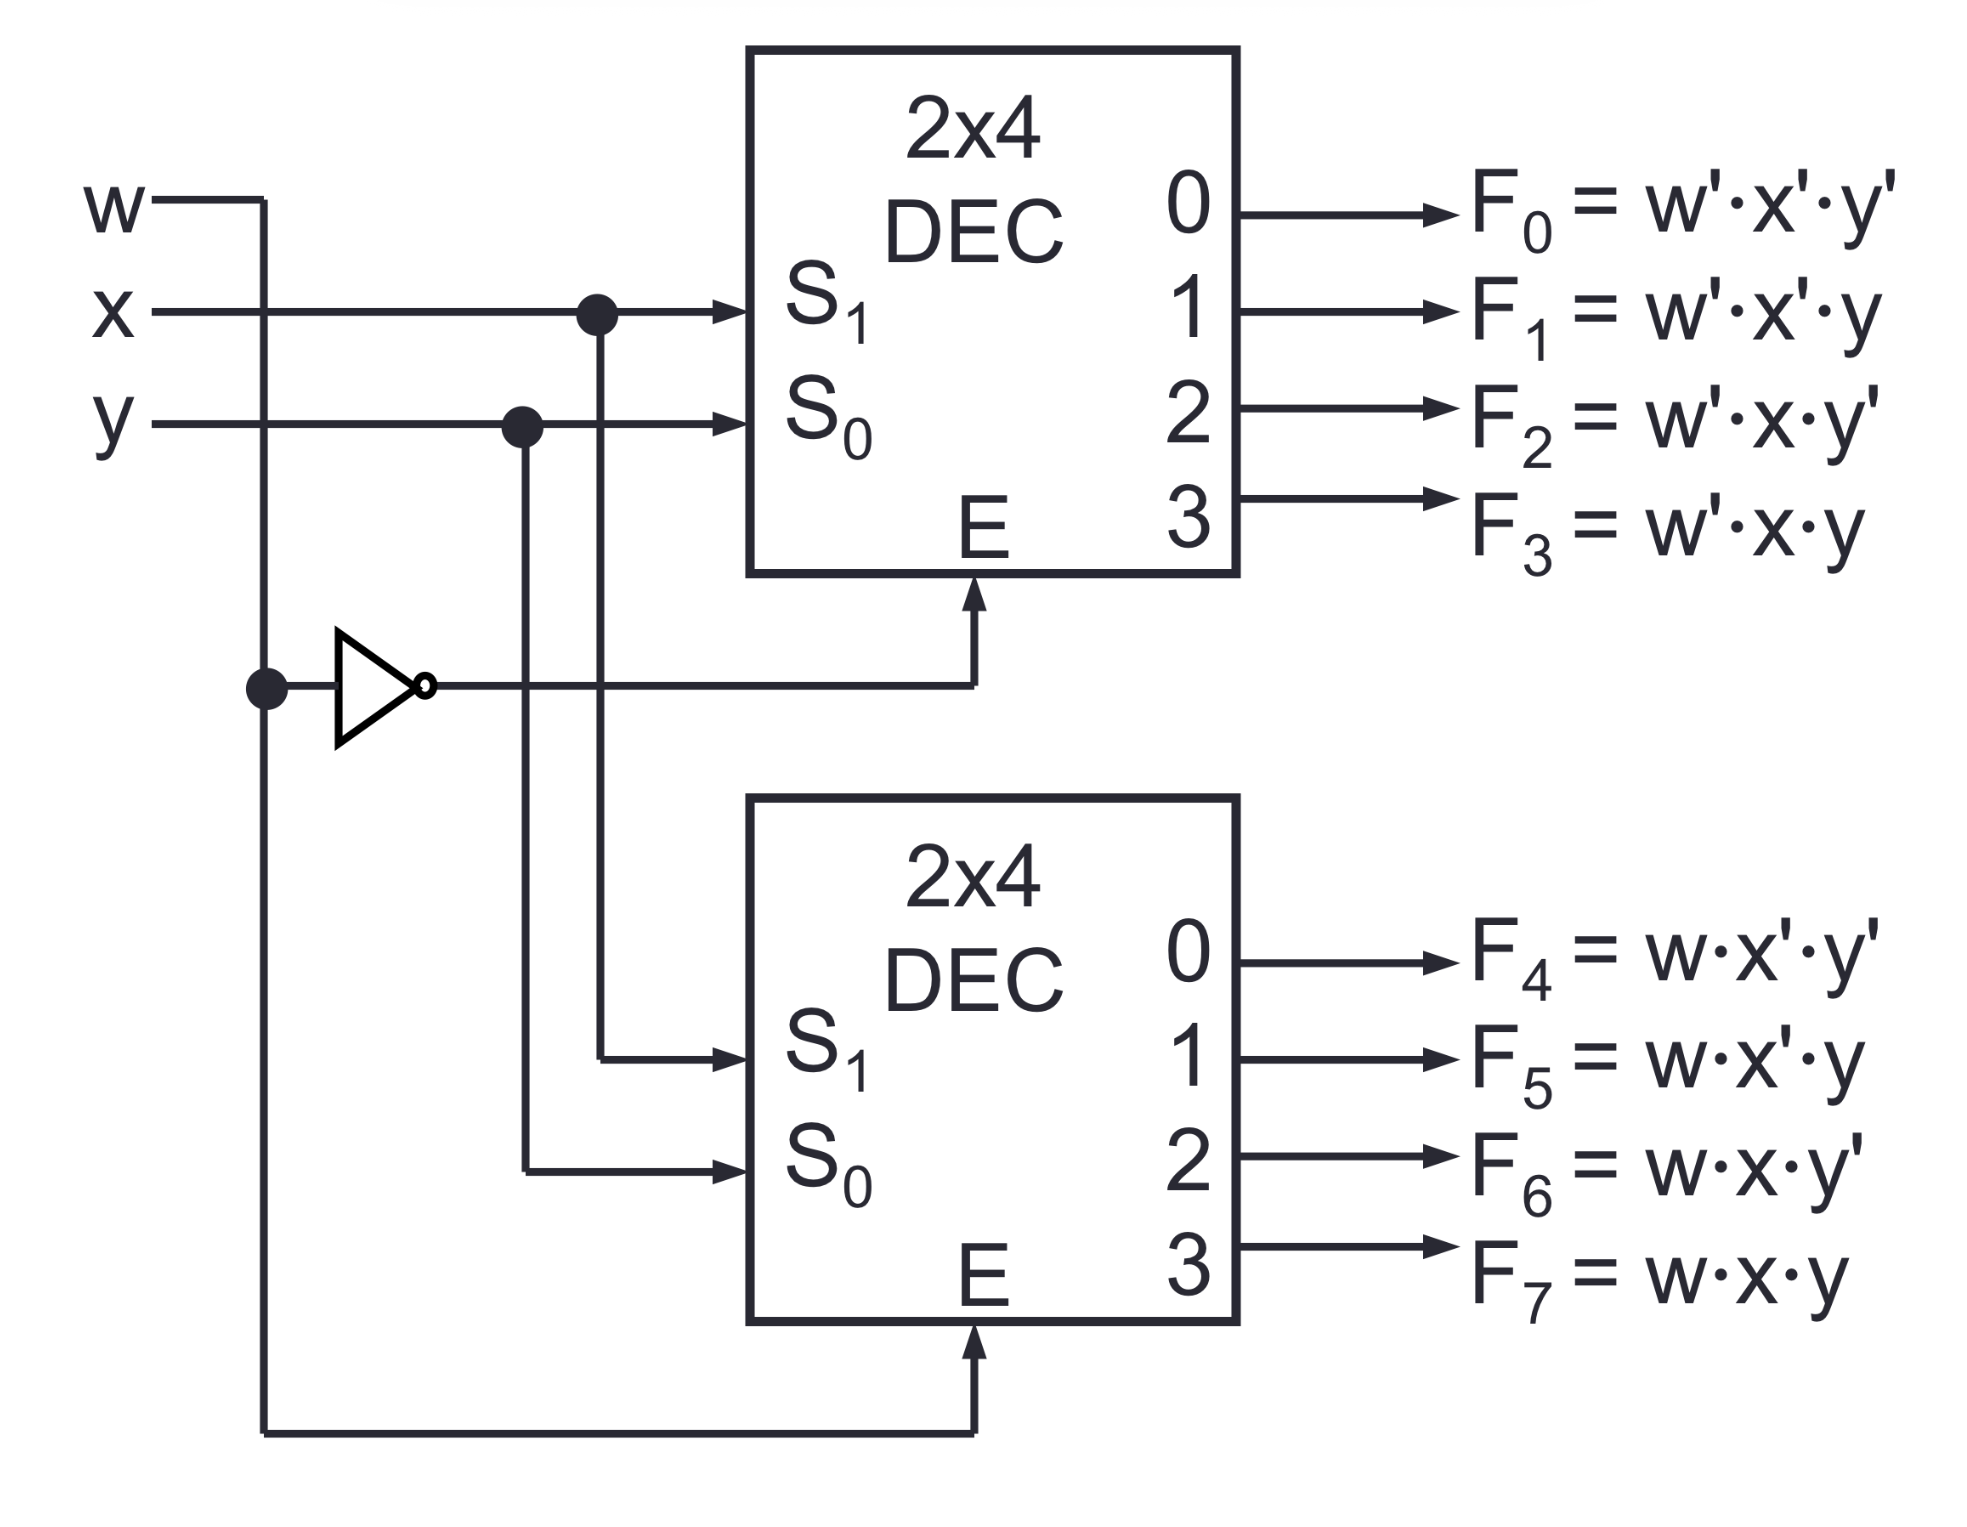
\includegraphics[width=0.3\textwidth]{decoder_cascade}
  \end{figure}
\end{example}
Decoders allow us to implement any function, by generating all the individual
minterms, and using an appropriate gate to implement the function. In general, for
a function $f=\sum m\left( a_1,a_2,\ldots,a_k \right)=\prod M\left(
b_1,b_2,\ldots,b_l \right)  $:
\begin{itemize}
  \item Decoder with active-high outputs
    \begin{itemize}
      \item with an OR gate:
        \[f=m_{a_1}+m_{a_2}+\cdots+m_{a_k}\]
      \item with a NOR gate:
        \[f=\left( m_{b_1}+m_{b_2}+\cdots+m_{b_l} \right)'\left[ =M_{b_1}\cdot
        \cdots \cdot M_{b_l} \right] \]
    \end{itemize}
  \item Decoder with active-low outputs
    \begin{itemize}
      \item with a NAND gate:
        \[f=\left( m_{a_1}'\cdot m_{a_2}'\cdot \cdots \cdot m_{a_k}\right)'\] 
      \item with an AND gate:
        \[f=m_{b_1}'\cdot m_{b_2}'\cdot \cdots \cdot m_{b_l}'.\] 
    \end{itemize}
\end{itemize}
They hence best lend themselves to circuits of many outputs, each a sum of a
few minterms. In general, any combinational circuit with $n$ inputs and $m$
outputs can be implemented with a $n:2^{n}$ decoder and $m$ logic gates. 

\paragraph{Encoders}
\begin{definition}[Encoders]
  A $m$-to-$n$-line, $m:n$, or $m\times n$ \textit{encoder}, converts binary
  information from $m<2^{n}$ input lines to $n$ output lines. If the $k$-th
  input line is active, the encoder outputs $\left( D_{n}D_{n-1}\cdots D_1
  \right)_2=k_{10}$. Behaviour is only defined for input lines of which exactly
  one is active.
\end{definition}
Encoders compute the inverse of decoders and can be implemented with $n$ OR
gates.
\begin{figure}[h!]
  \centering
  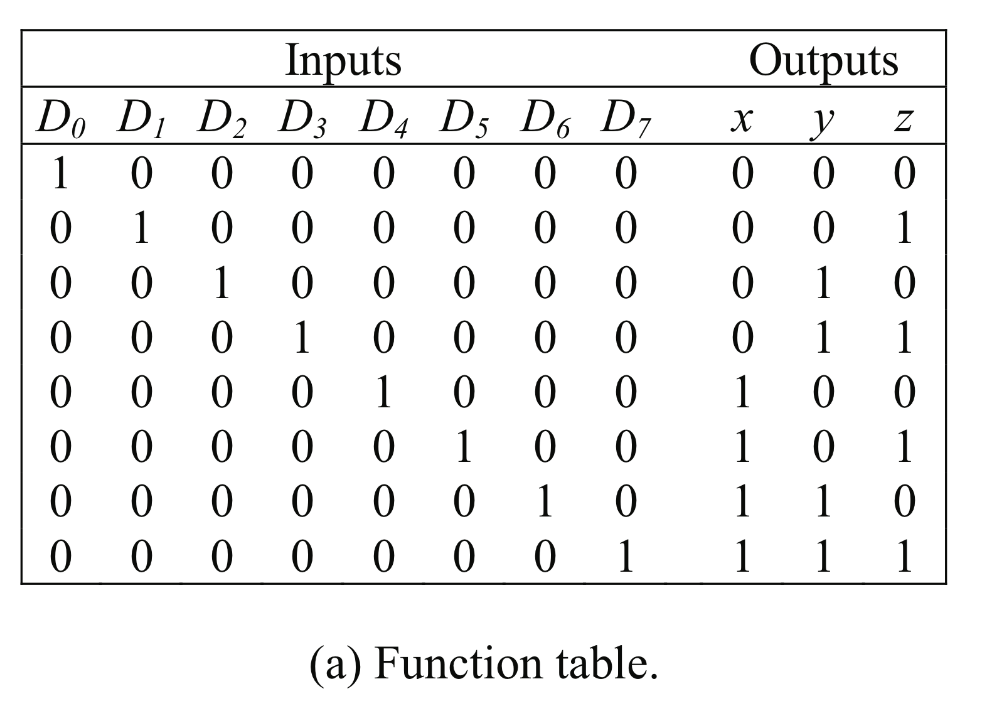
\includegraphics[width=0.4\textwidth]{encoder_truth}
  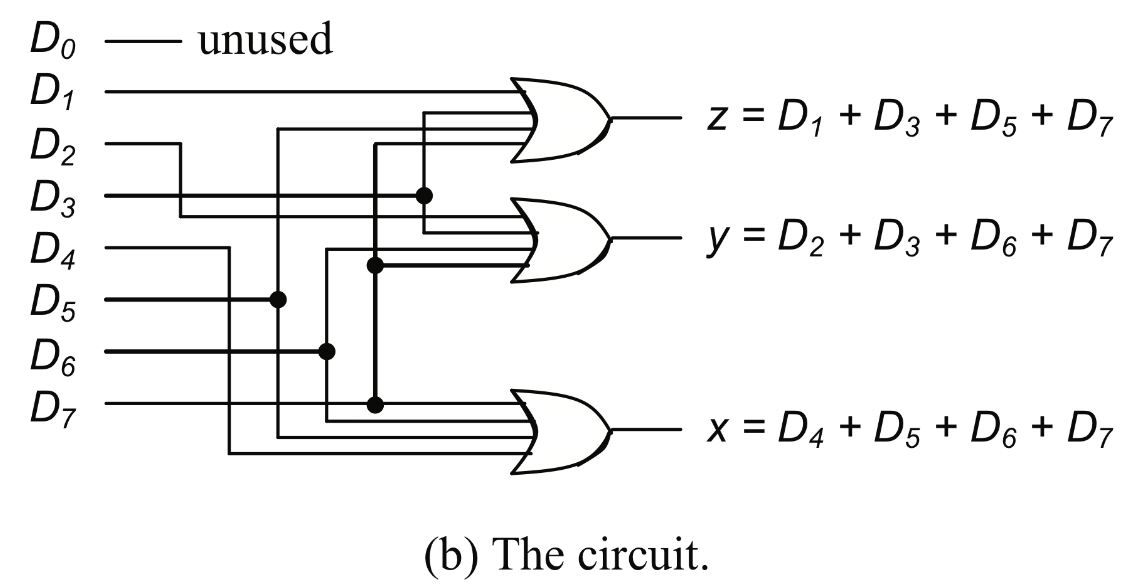
\includegraphics[width=0.4\textwidth]{encoder_circuit}
\end{figure}

\begin{definition}[Priority Encoders]
  A \textit{priority encoder} is an encoder with priority. If two or more
  outputs are active, the input with the highest priority takes precedence. If
  all inputs are inactive, behaviour is undefined.
\end{definition}

\paragraph{Demultiplexers}
\begin{definition}[Demultiplexers]
  Given an input line and a set of selection lines, a
  \textit{demultiplexer} directs data from the input to one selected output line
  by the control signals.
\end{definition}
\begin{figure}[h!]
  \centering
  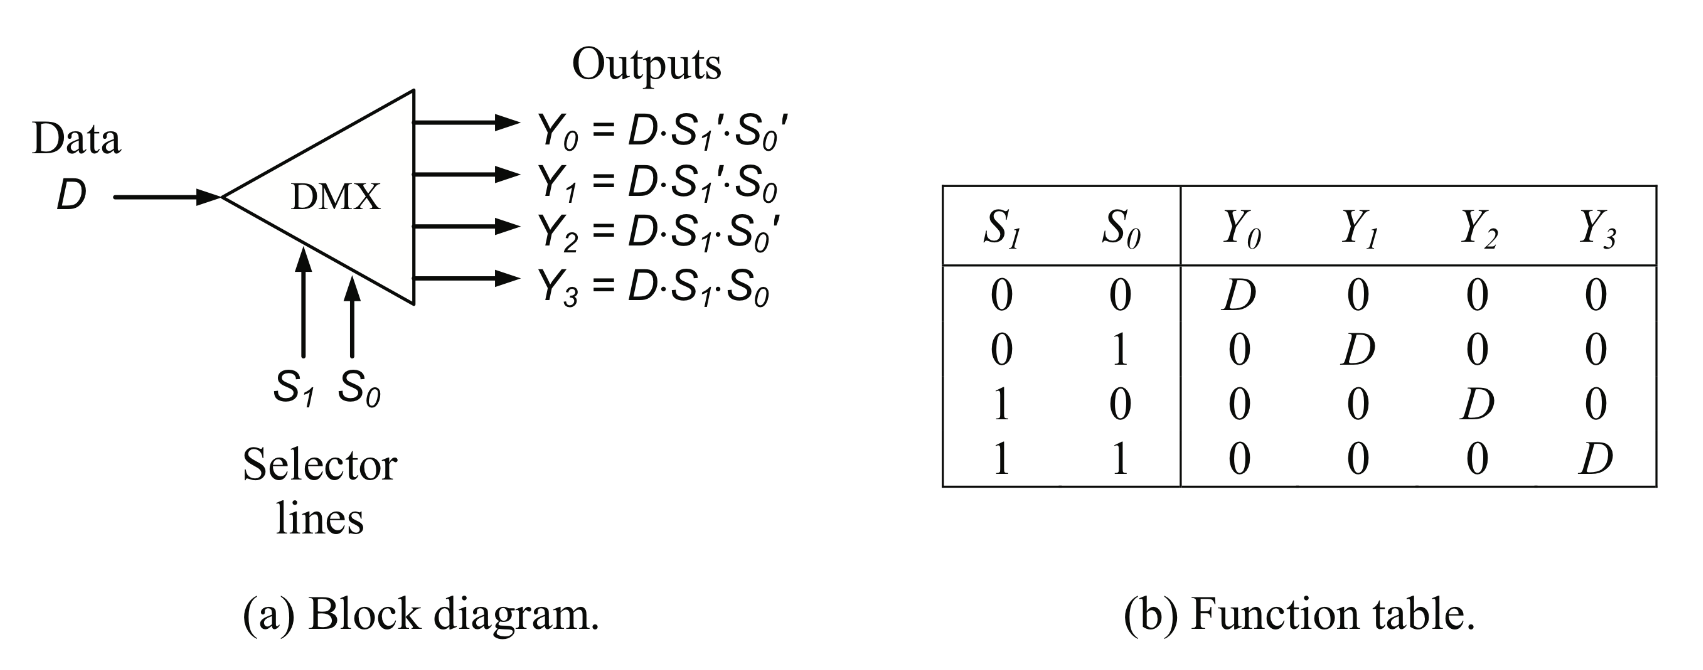
\includegraphics[width=0.6\textwidth]{demultiplexer}
\end{figure}
The demultiplexer circuit is identical to a decoder with enable, by taking the
enable as the input and the input lines as the control.

\paragraph{Multiplexers}
\begin{definition}[Multiplexers]
  A \textit{multiplexer}, or data-selector, has $2^{n}$ input lines, $n$
  selection or control lines, and one output line. It directs data from the
  specified input line to the output line.
\end{definition}
It may be implemented with a $n:2^{n}$decoder, and getting each of the $2^{n}$
output's  product with the corresponding input line.

\begin{example}[74151A $8:1$ Multiplexer]
  We illustrate the representations of a standard 74151A multiplexer.
  \begin{figure}[h!]
    \centering
    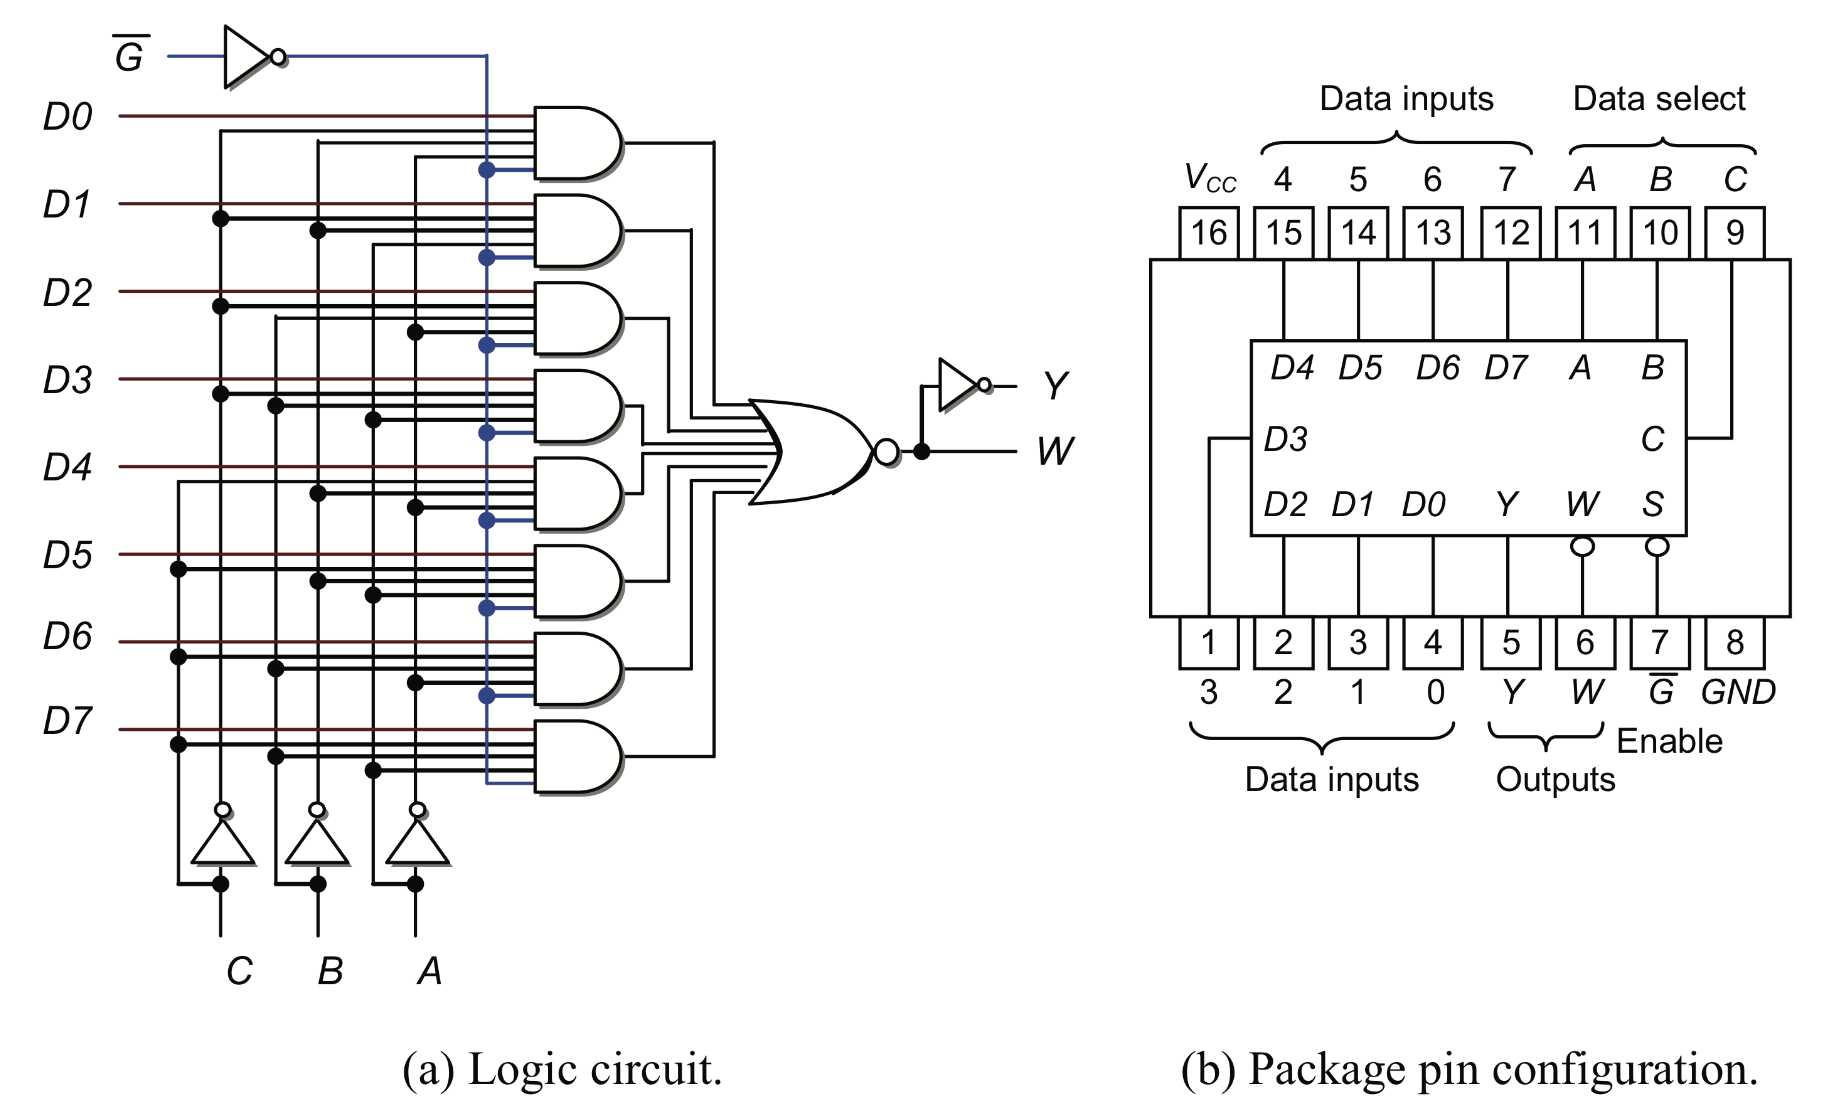
\includegraphics[width=0.4\textwidth]{multiplexer}
    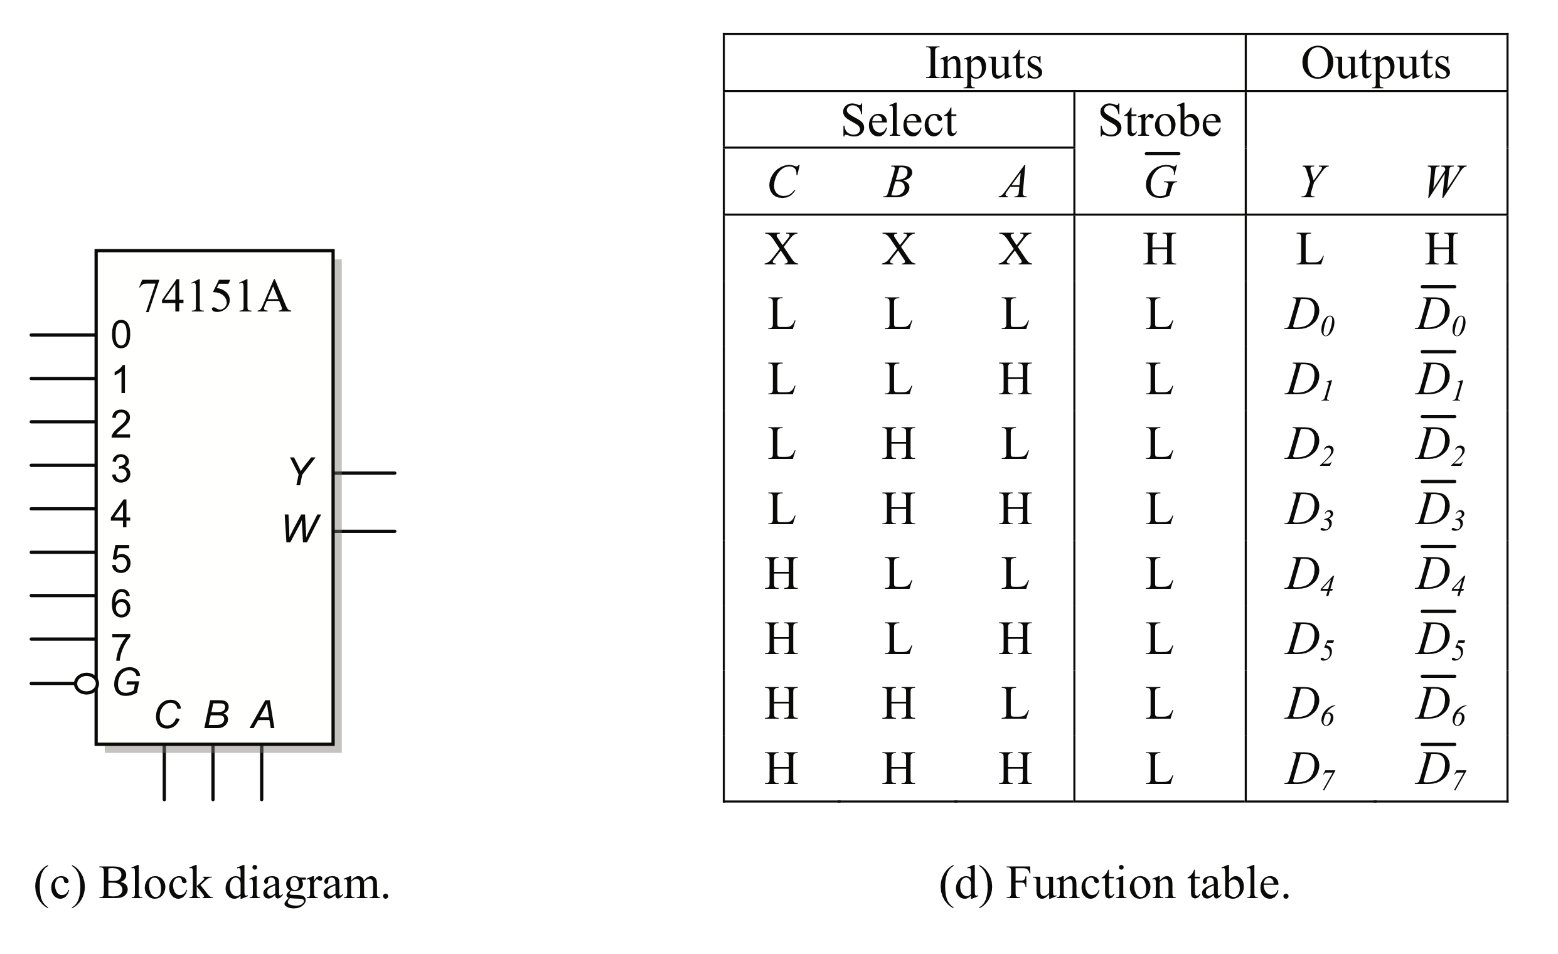
\includegraphics[width=0.4\textwidth]{multiplexer_2}
  \end{figure}
\end{example}

Multiplexers can also be cascaded to construct larger multiplexers.
\begin{example}[$8:1$ Multiplexer] We can construct a $8:1$ multiplexer from
  smaller multiplexers as shown.
  \begin{figure}[h!]
    \centering
    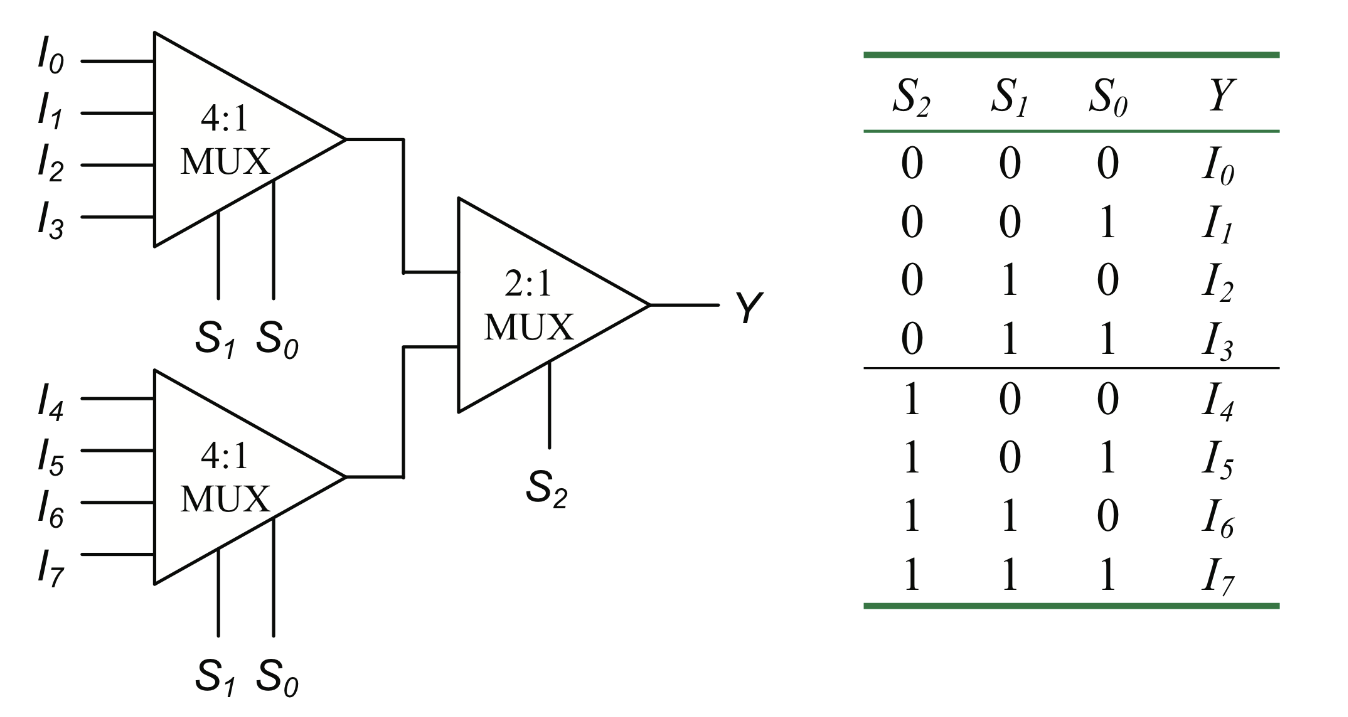
\includegraphics[width=0.4\textwidth]{multiplexer_cascade}
    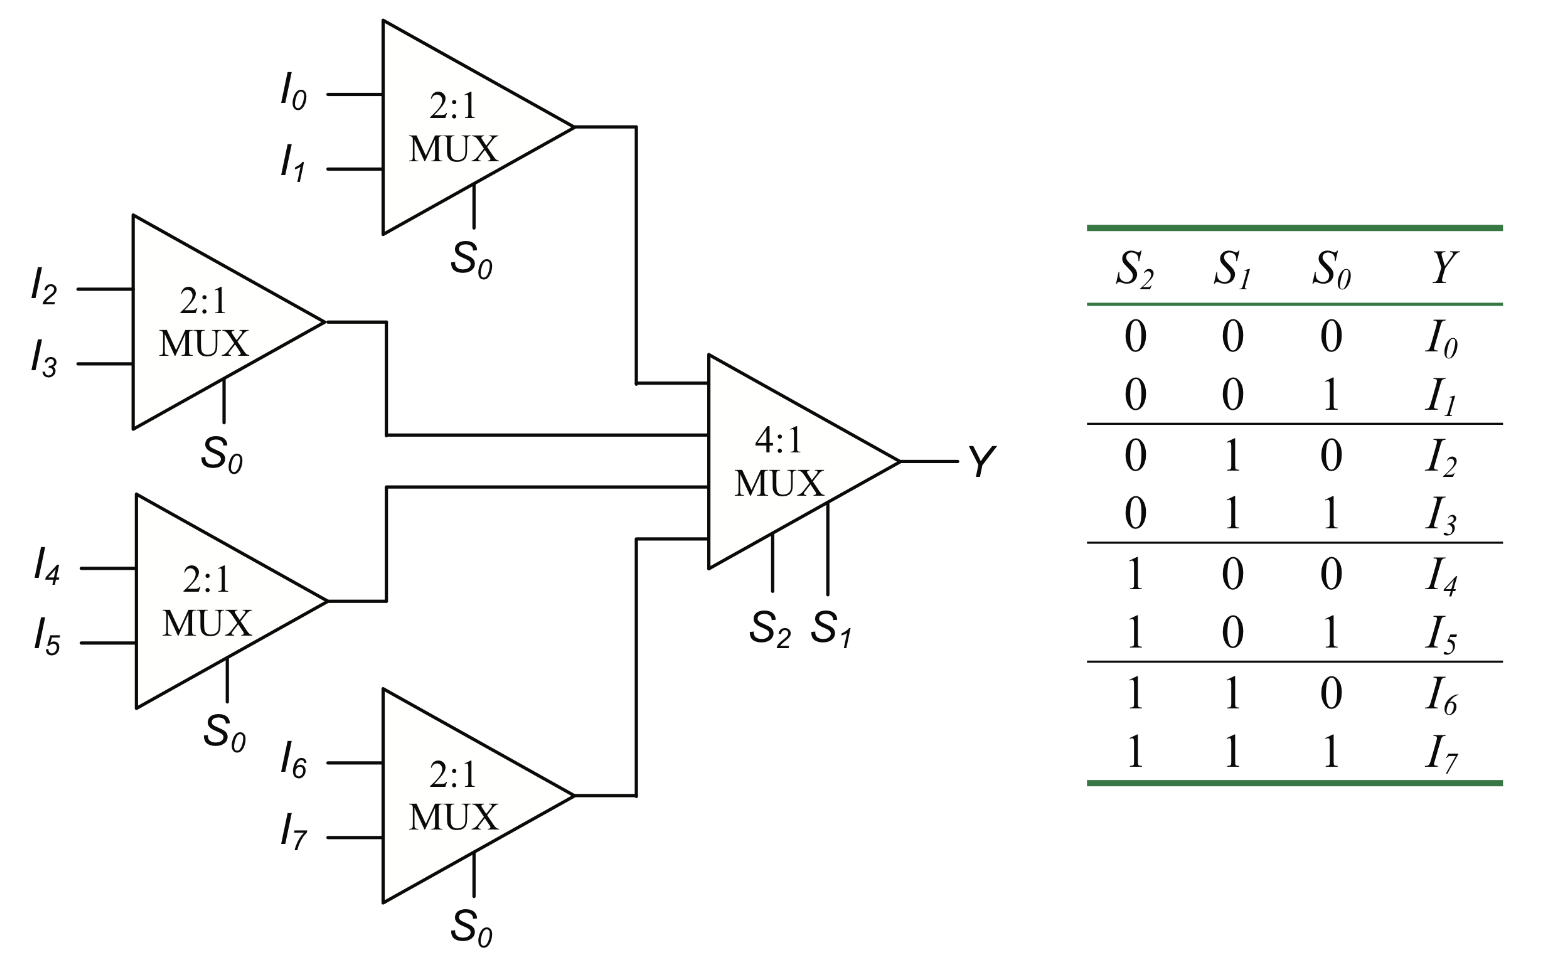
\includegraphics[width=0.45\textwidth]{multiplexer_cascade_2}
  \end{figure}
\end{example}

Multiplexers also allow us to implement any function, by having each of the
variables as a selection line, and setting each input to be $1$ if it is the
$k$-th line, where $m(k)$ is a minterm of the function and $0$ otherwise. We
may also implement a $n$-variable function with a $2^{n-1}:1$ multiplexer, by
setting one of the variables to be input and the others the selection lines. We
do so by drawing the truth table, grouping by selection line values, and then
comparing the input variable to the function output.\\

We illustrate this with the following example, where $f(A,B,C)=\sum m\left(
0,1,3,6 \right) $.
\begin{figure}[h!]
  \centering
  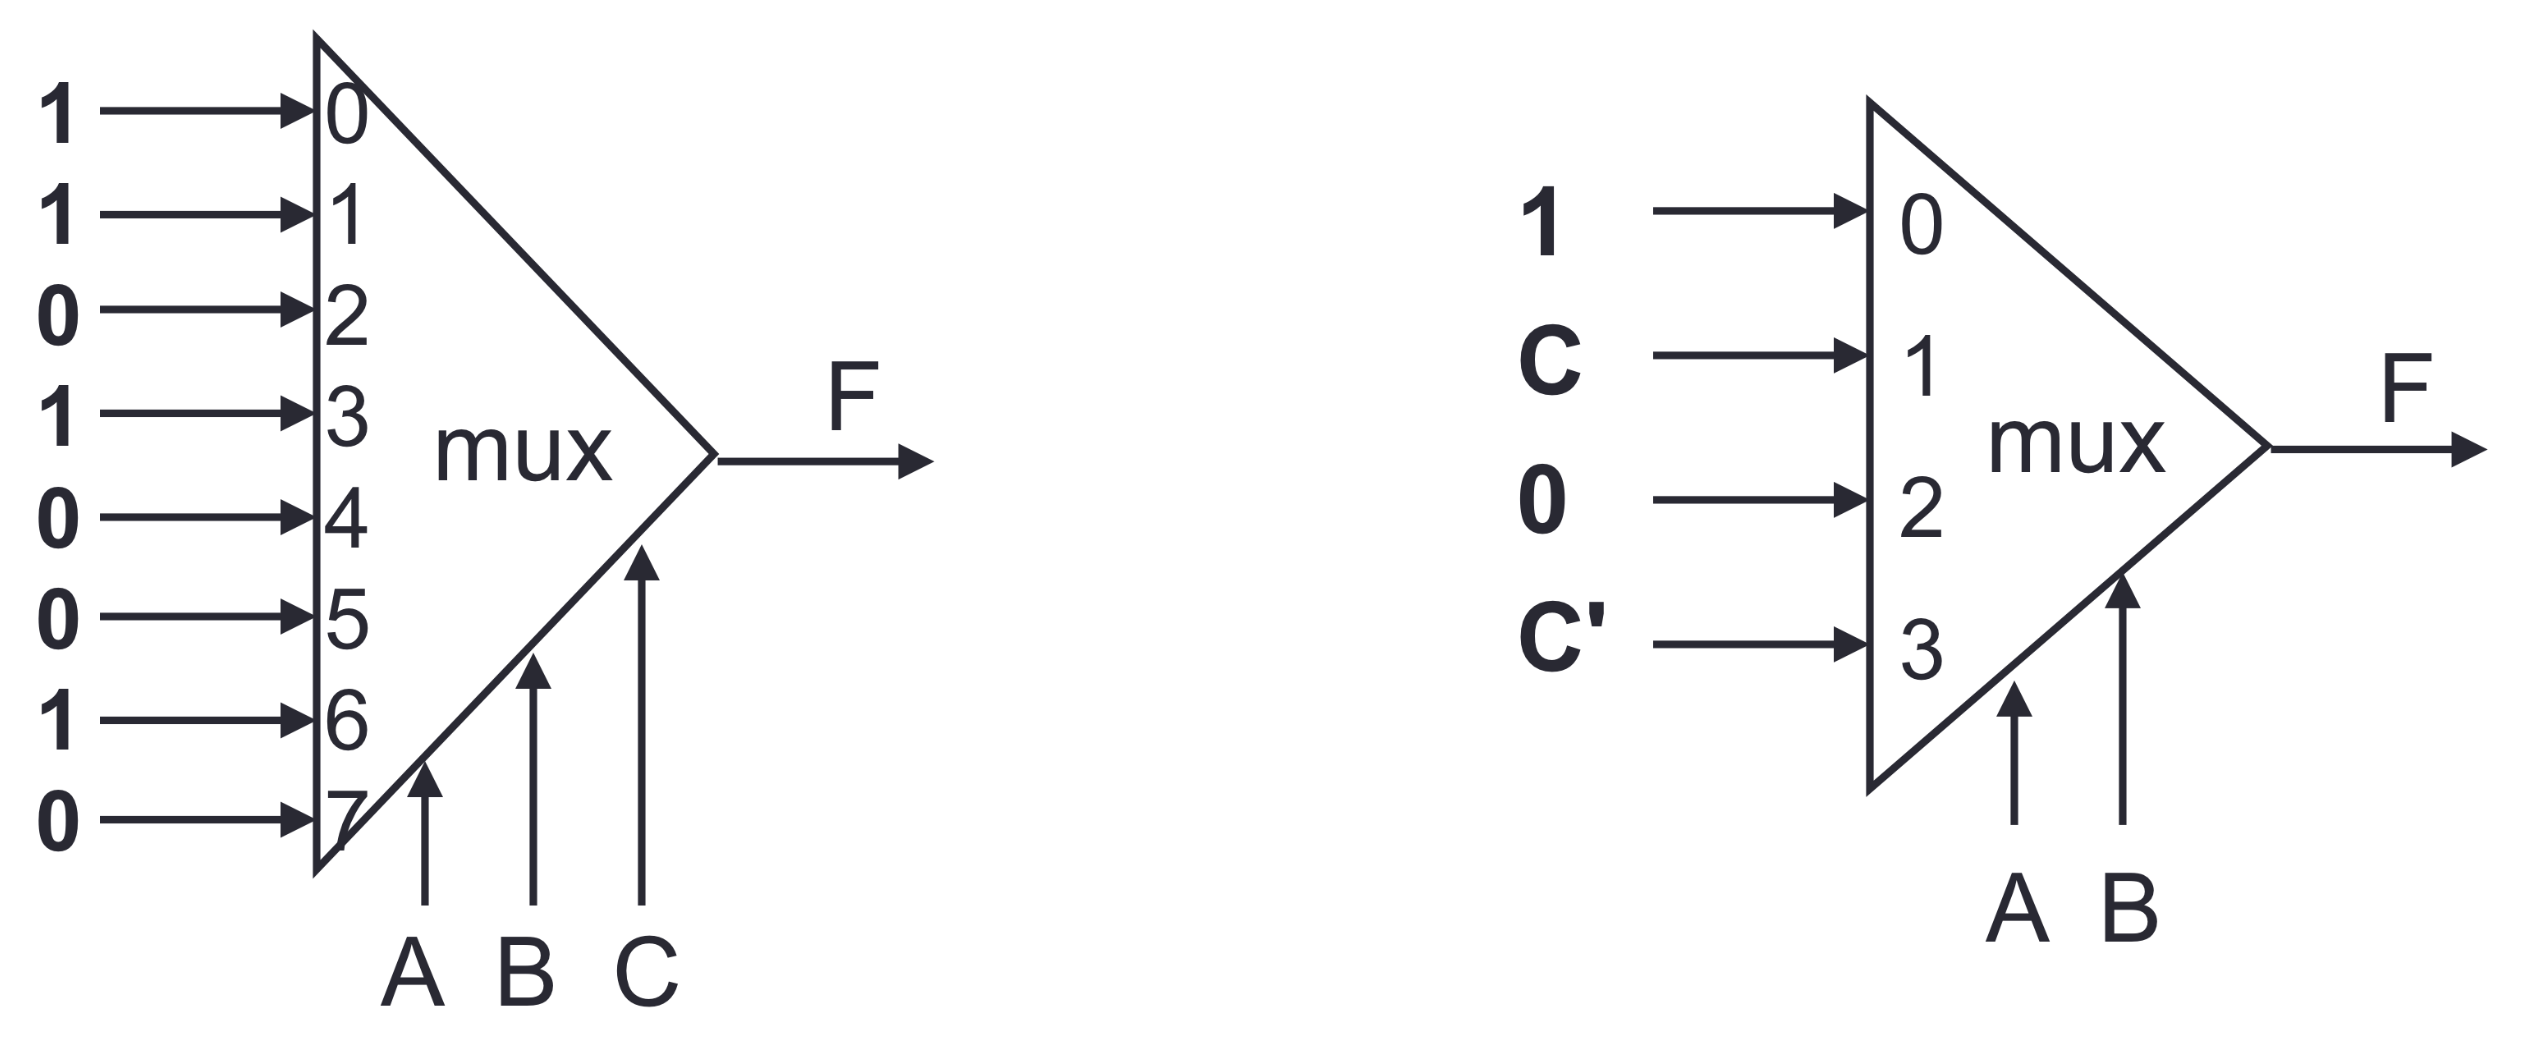
\includegraphics[width=0.35\textwidth]{multiplexer_imp_2}
  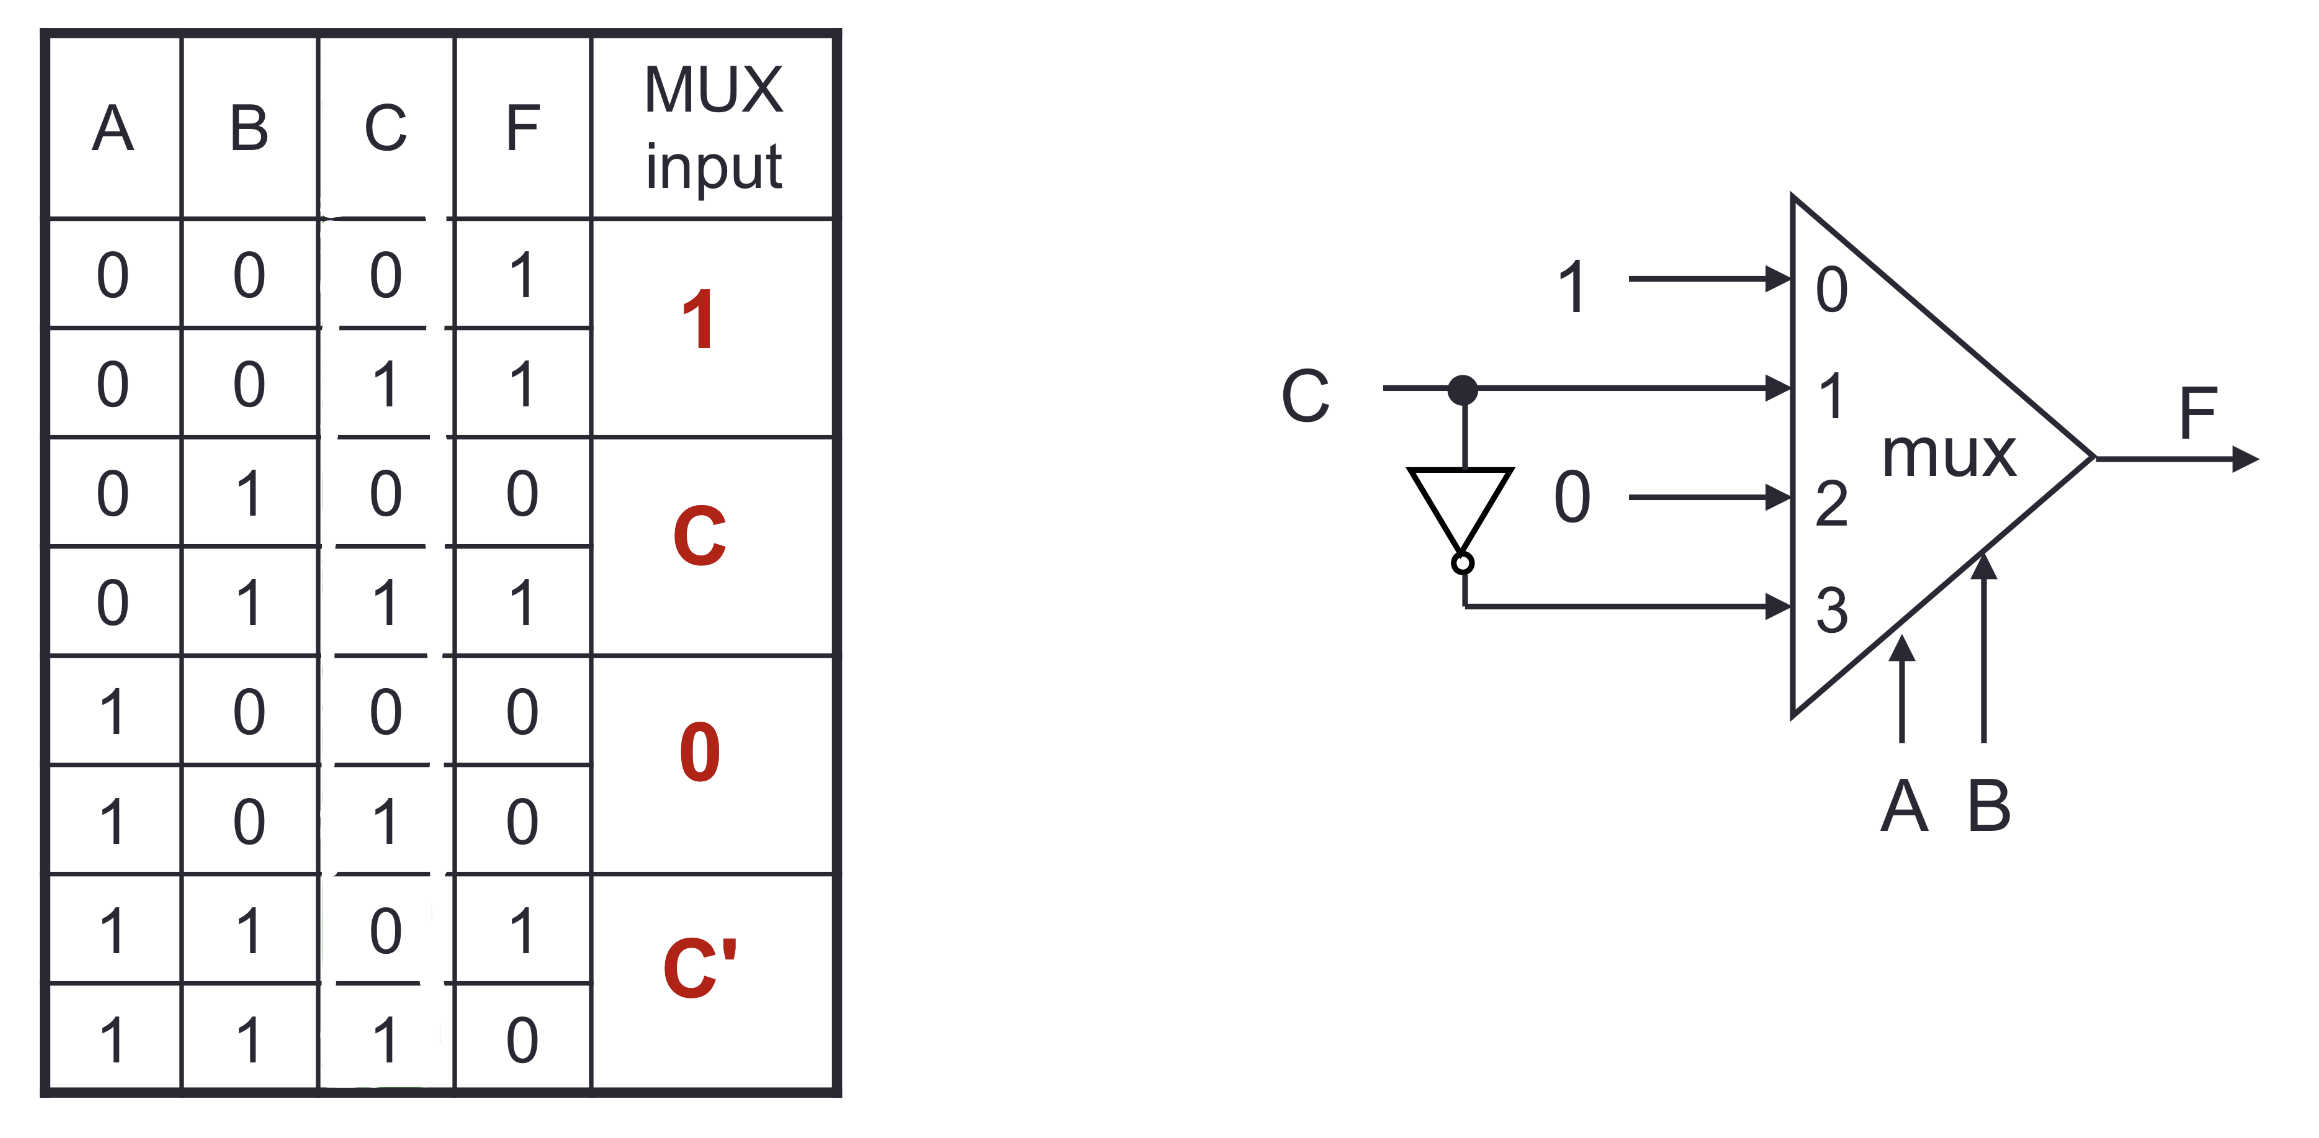
\includegraphics[width=0.45\textwidth]{multiplexer_imp}
\end{figure}


\subsection{Combinational Circuits}
Within logic circuits, we first consider the class of combinational circuits,
where each output depends on only the immediate inputs. We may implement
combinational circuits with logic gates in the \textbf{gate-level design
method}, or functional blocks in the \textbf{block-level design method}.\\

\subsubsection{Gate-Level (SSI) Design}
In gate-level design, we follow the design procedure of (1) Stating the
problem, (2) Determining and labelling the inputs and outputs, (3) Drawing the
truth table, (4) Obtaining simplified Boolean expressions, (5) Drawing the
logic diagram.

\begin{example}[Full Adder] We demonstrate the design procedure with the Full
  Adder component.
  \begin{definition}[Half Adders]
    A \textit{Half Adder} is a circuit that adds 2 single bits $X$ and $Y$ to
    produce a result the carry-out bit $C$ and the sum bit $S$.
  \end{definition}
  From the truth table and algebraic simplification, we derive the simplified
  expressions for $C$ and $S$
  \[C=X\cdot Y,\qquad S=S'\cdot Y+X\cdot Y'=X\oplus Y.\]
  \begin{figure}[h!]
    \centering
    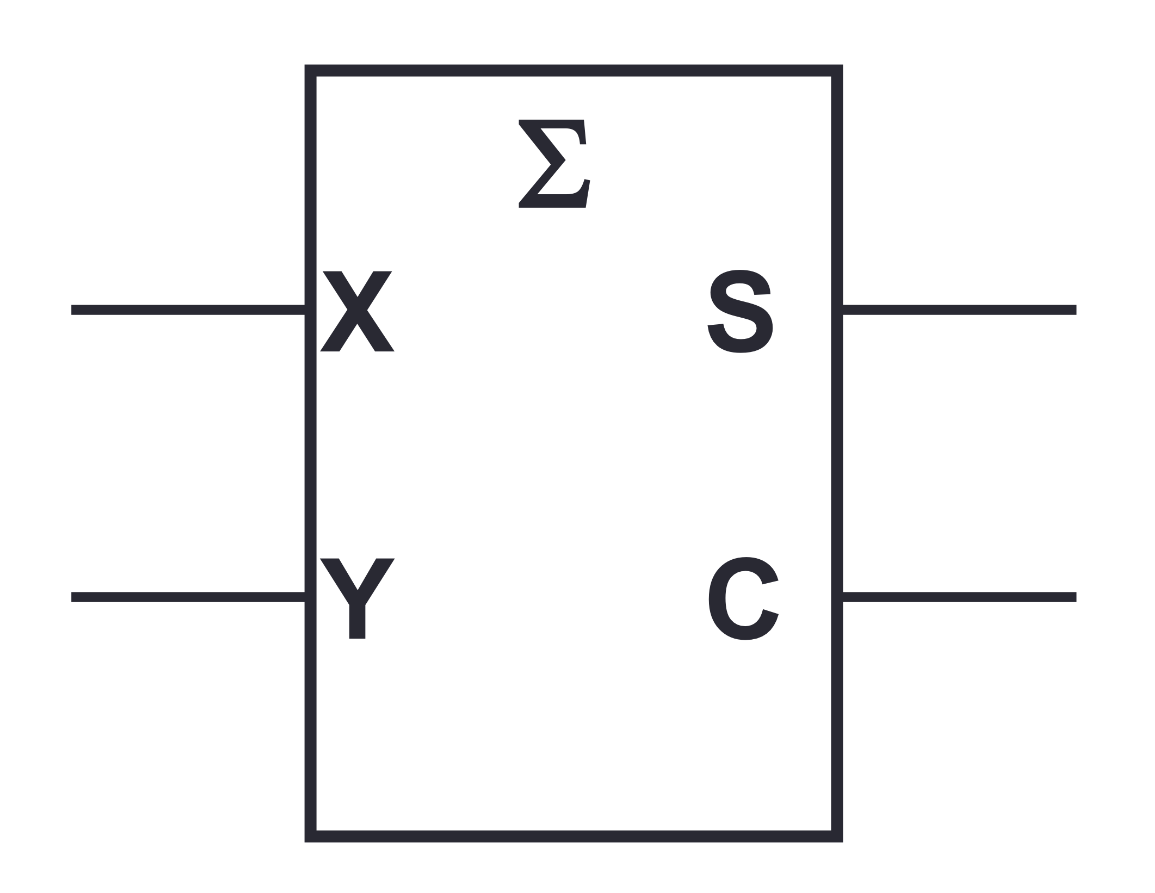
\includegraphics[height=0.15\textwidth]{half_adder_block}
    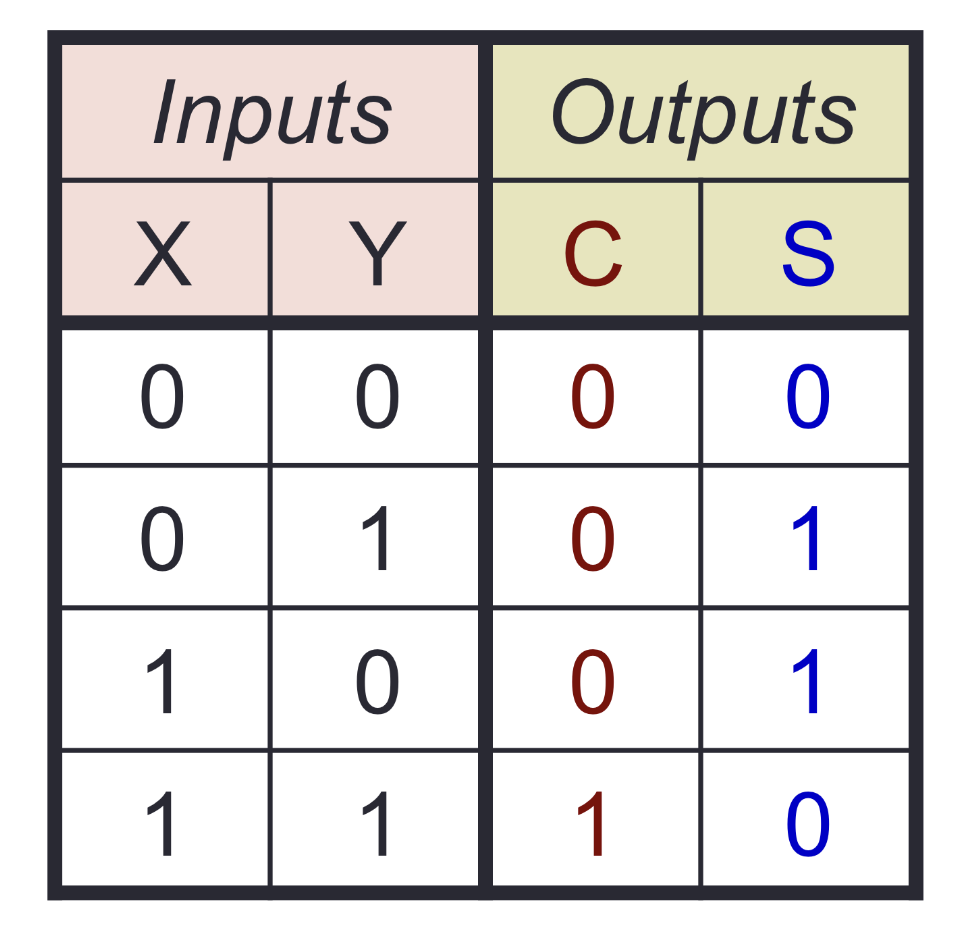
\includegraphics[height=0.15\textwidth]{half_adder_truth}
    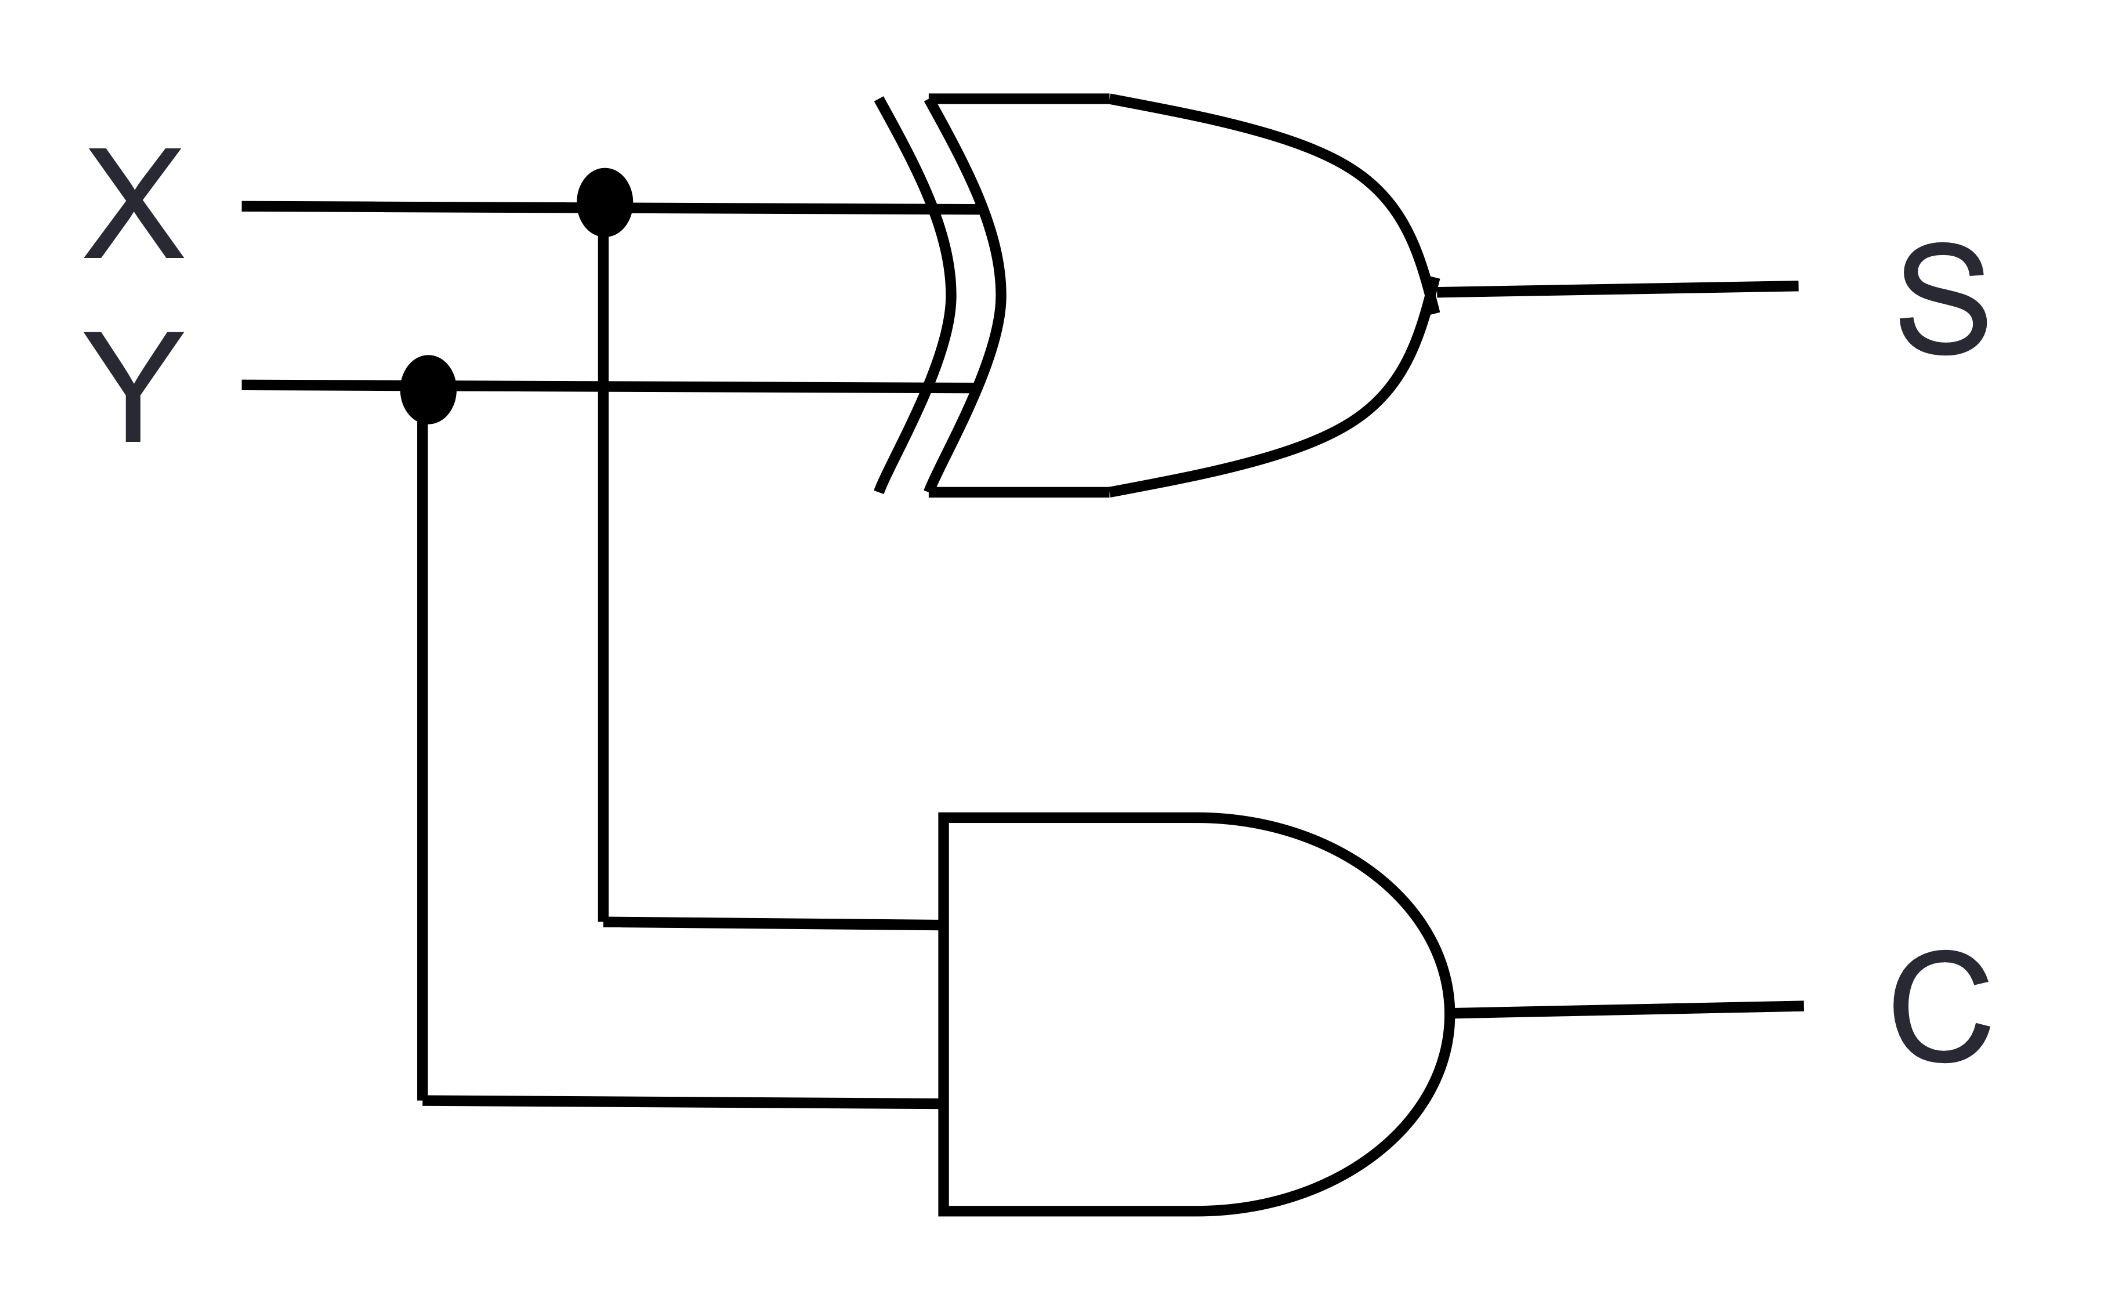
\includegraphics[height=0.15\textwidth]{half_adder_circuit}
  \end{figure}\\
  We aim to obtain a full-adder to be able to add 3 single bits, which we call
  $X$, $Y$, and a carry-in bit $Z$. Using the K-map, we have the simplified SOP
  forms
  \[C=X\cdot Y+X\cdot Z+Y\cdot Z=X\cdot Y+\left( X\oplus Y \right)\cdot Z\]
  \[S=X'\cdot Y'\cdot Z+X'\cdot Y\cdot Z'+X\cdot Y'\cdot Z'+X\cdot Y\cdot Z=X\oplus\left( Y\oplus Z \right).\] 
  \begin{figure}[h!]
    \centering
    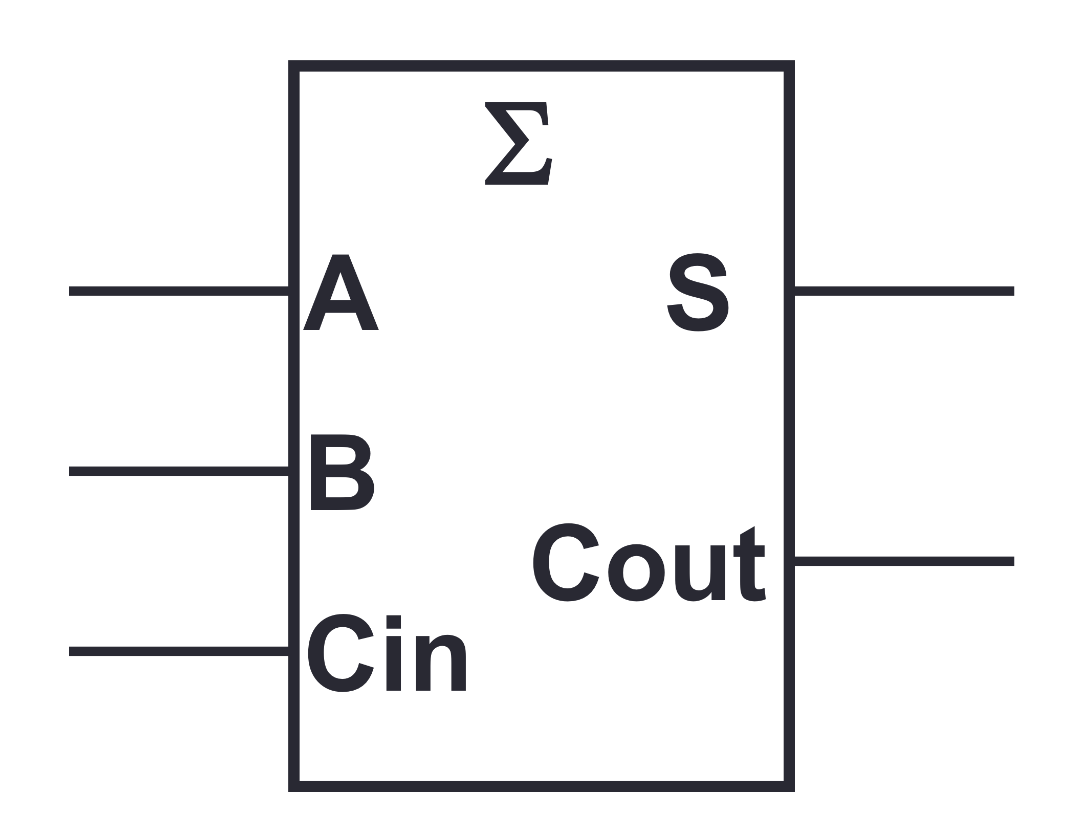
\includegraphics[height=0.2\textwidth]{full_adder_block}
    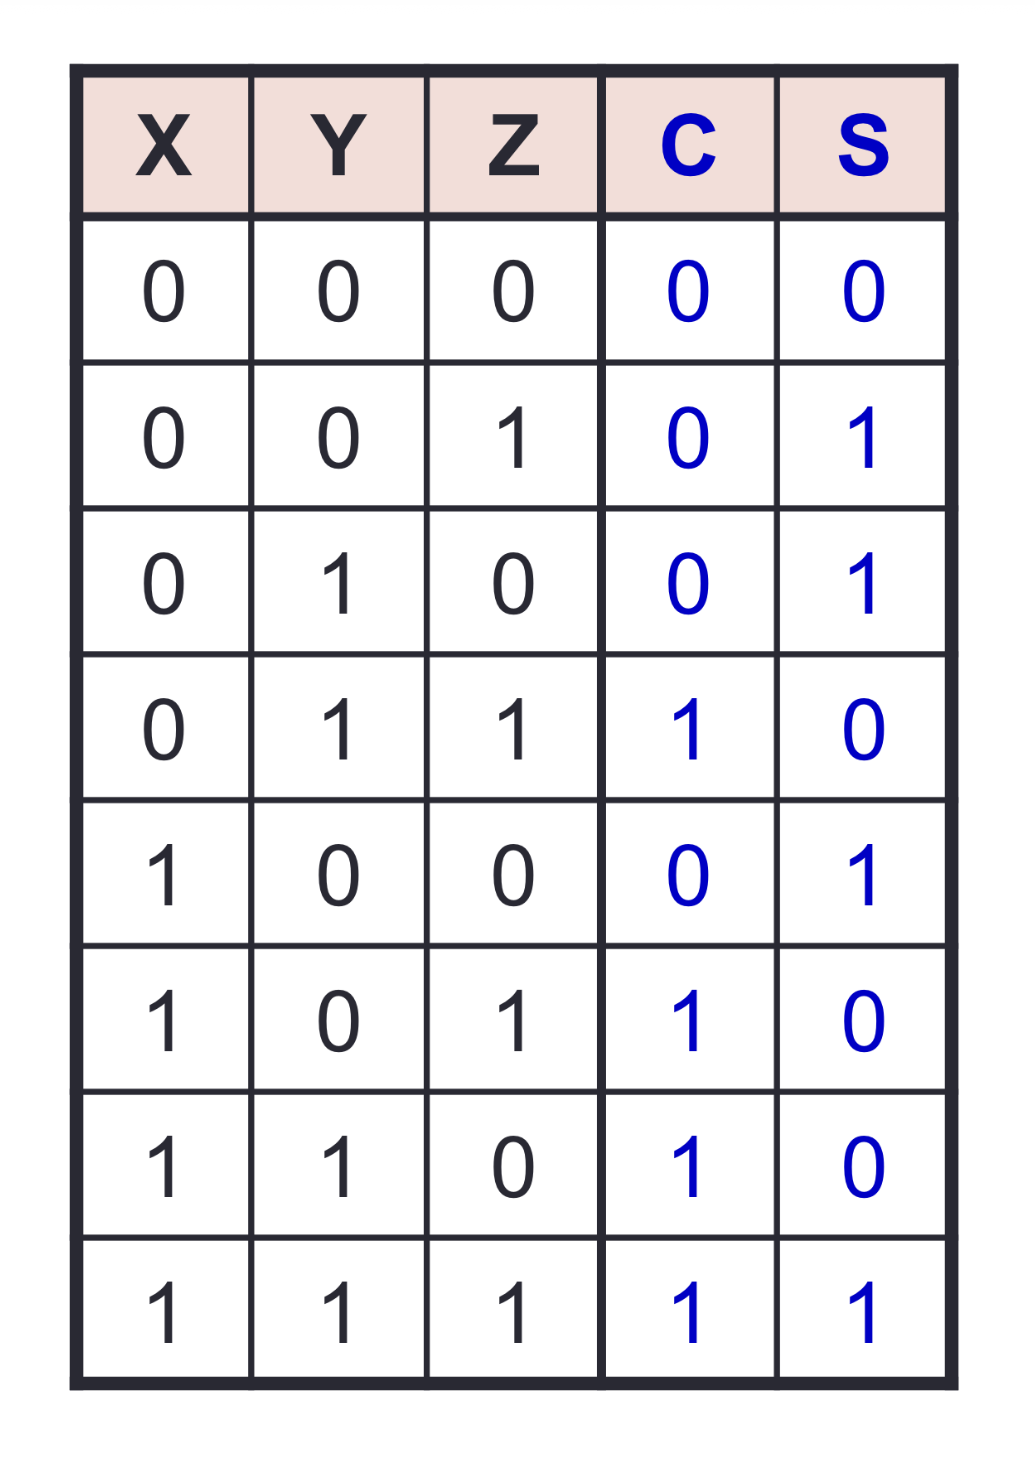
\includegraphics[height=0.2\textwidth]{full_adder_truth}
    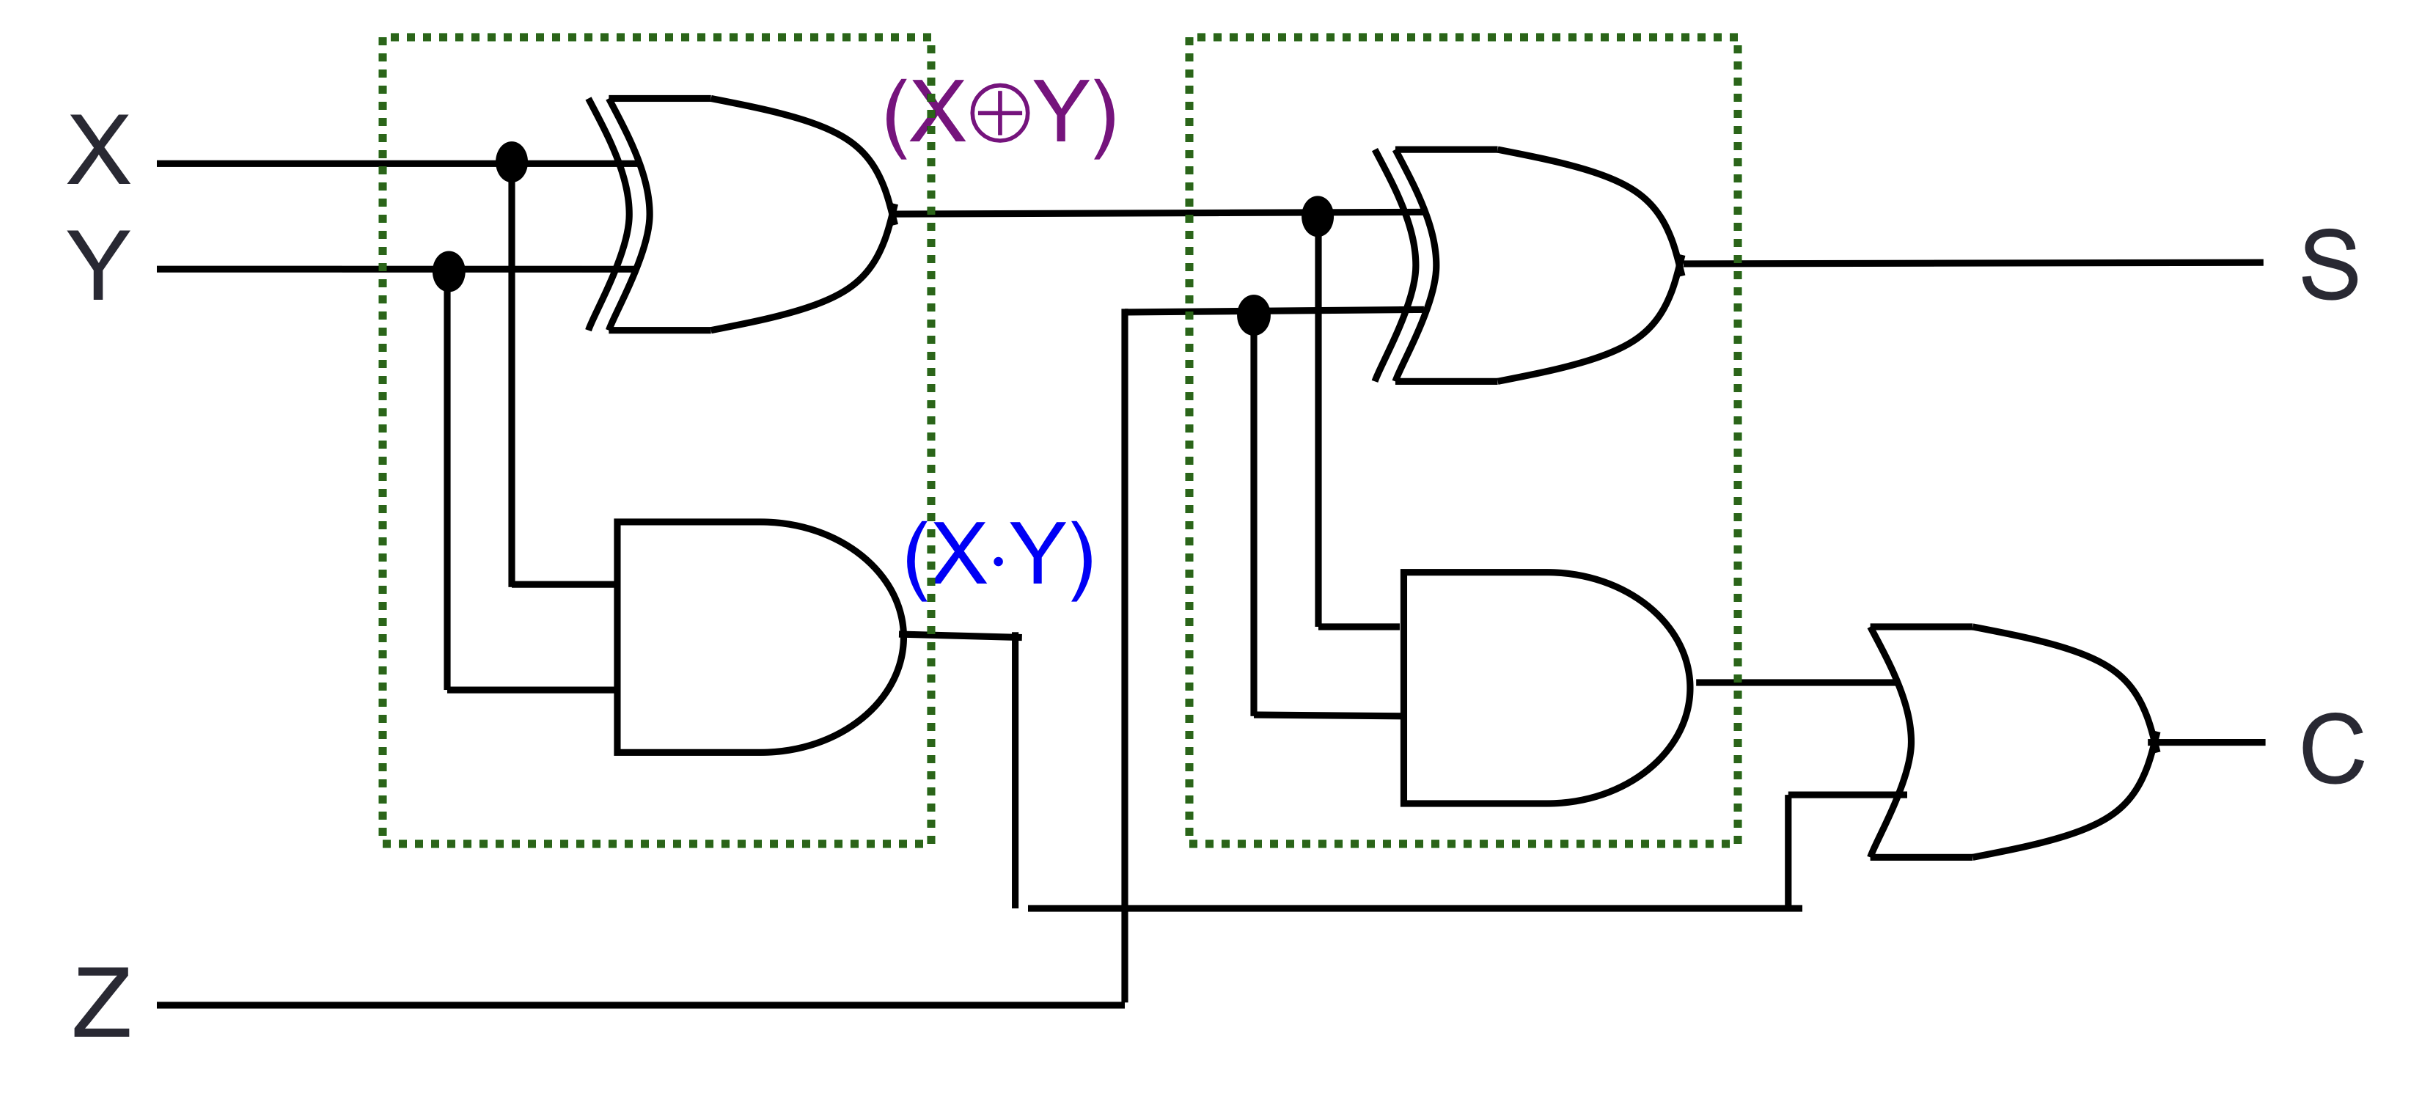
\includegraphics[height=0.2\textwidth]{full_adder_circuit}
  \end{figure}\\
  We hence have the full adder constructed from two half-adders and an OR gate.
\end{example}

\subsubsection{Block-Level Design}
For more complex circuits, we may employ block-level design, where we decompose
the main problem to sub-problems recursively to be directly solved by blocks of
circuits.

\begin{example}[Parallel Adder] We demonstrate the block-level design procedure
  with the paralllel adder component.
  \begin{definition}[Parallel Adders]
    A \textit{parallel adder} is a circuit that adds two $4$-bit numbers $X=X_4
    X_3 X_2 X_1$ and $Y=Y_4 Y_3 Y_2 Y_1$ and a carry-in bit $C_1$ to produce a
    $5$-bit result $R=C_5S_4S_3S_2S_1$
  \end{definition}
  Rather than drawing a truth table with $9$-bit inputs, we notice the addition
  formula for each pair of bits with carry-in has the same function as a full
  adder
  \[C_{i+1} S_i=X_i+Y_i+C_i\]
  \[C_{i+1}=X_i\cdot Y_i+\left( X_i\oplus Y_i \right)\cdot  C_i,\qquad
  S_i=X_i\oplus Y_i\oplus C_i.\] 
  This allows us to cascade full adders via their carries to create a
  \textit{parallel adder} (or \textit{ripple-carry adder}).
  \begin{figure}[h!]
    \centering
    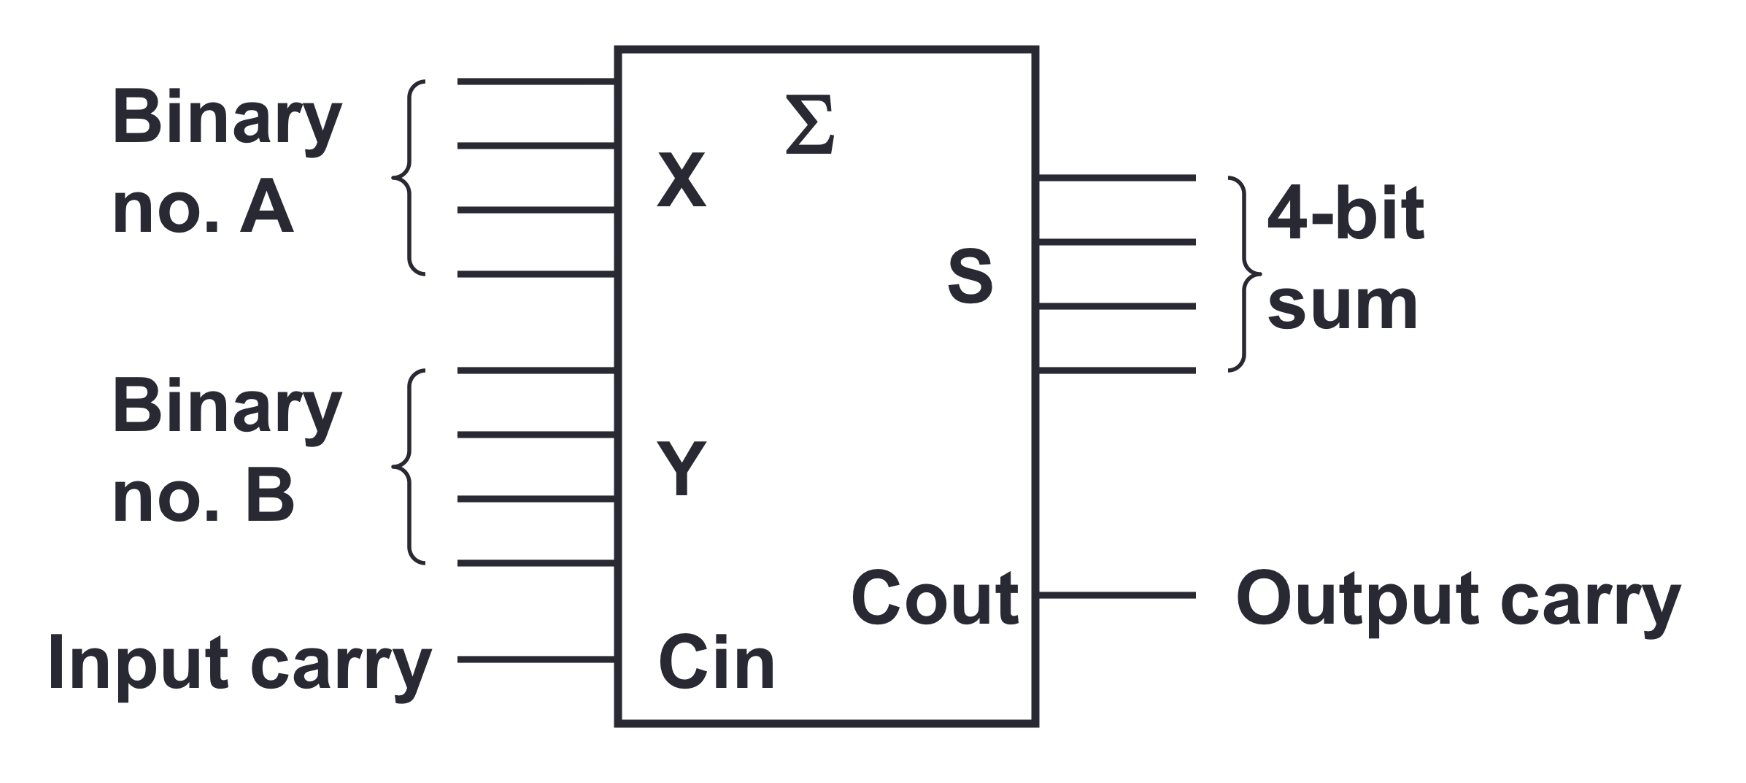
\includegraphics[height=0.2\textwidth]{parallel_adder_block}
    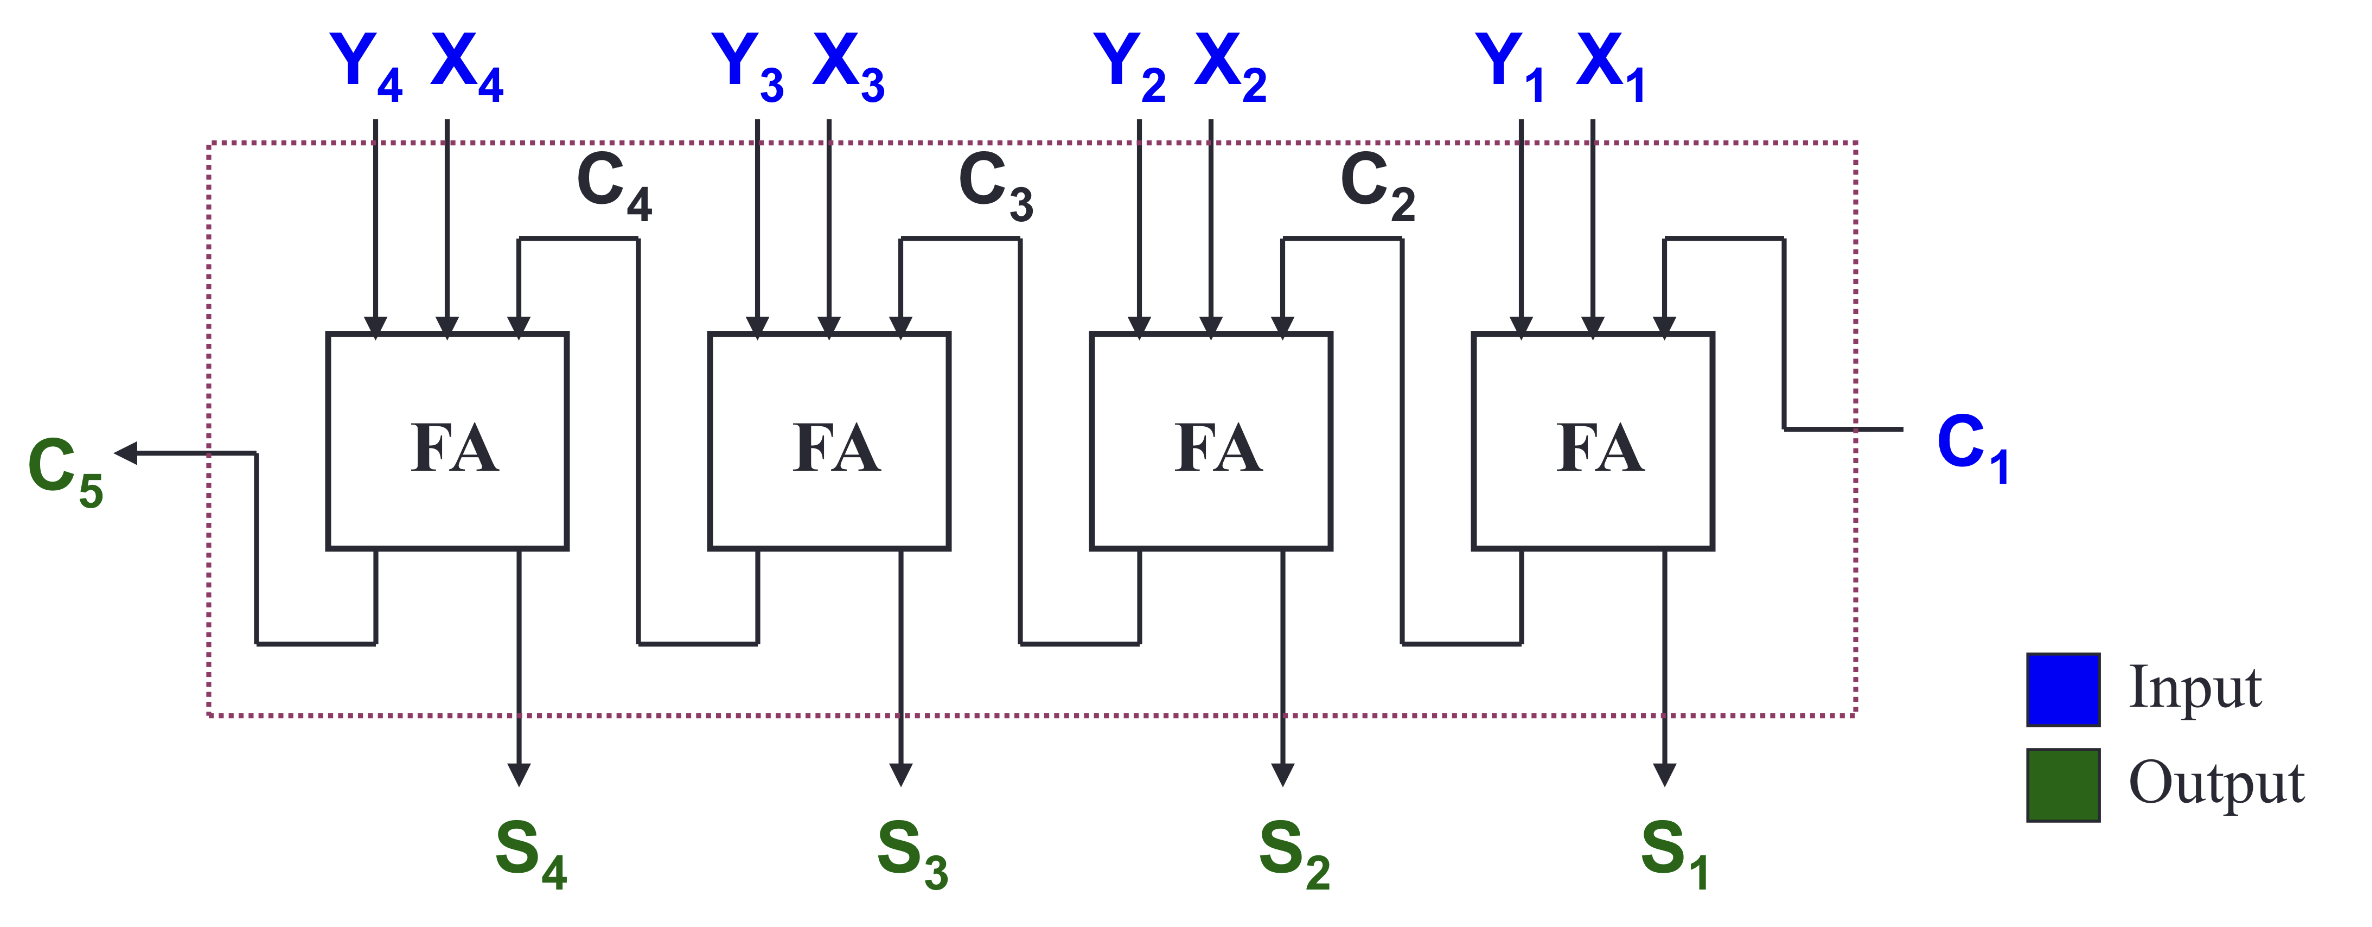
\includegraphics[height=0.2\textwidth]{parallel_adder_circuit}
  \end{figure}\\
\end{example}
Given the $4$-bit parallel adder, we may much more easily
implement a BCD to Excess-$k$ converter (by adding $k$ to a given BCD), or a
$4n$-bit parallel adder (by similarly cascading $n$ parallel adders).
\begin{remark}
  The circuit delay of a ripple-carry parallel adder is proportional to the
  number of bits it handles, since the carry bits has to propagate through each
  full adder.
\end{remark}

\begin{example}[Magnitude Comparator]
  Alternatively, to design a more complicated circuit, we may analyse the
  formulae or algorithms in its computation.
  \begin{definition}[Magnitude Comparators]
    A $n$-bit \textit{magnitude comparator} is a circuit that, given two
    $n$-bit numbers $A$ and $B$, compares and returns either $A>B$, $A=B$, or
    $A<B$.
  \end{definition}
  Given two unsigned values $A$ and $B$, we are only required to compare the
  MSB of the two values to conclude $A<B$ or vice versa, and check the next MSB
  only if the current MSB is equal. We hence may obtain the following circuit,
  where $A=A_3A_2A_1A_0$, $B=B_3B_2B_1B_0$, and $x_i=A_i\cdot B_i+A_i'\cdot
  B_i'$.
  \begin{figure}[h!]
    \centering
    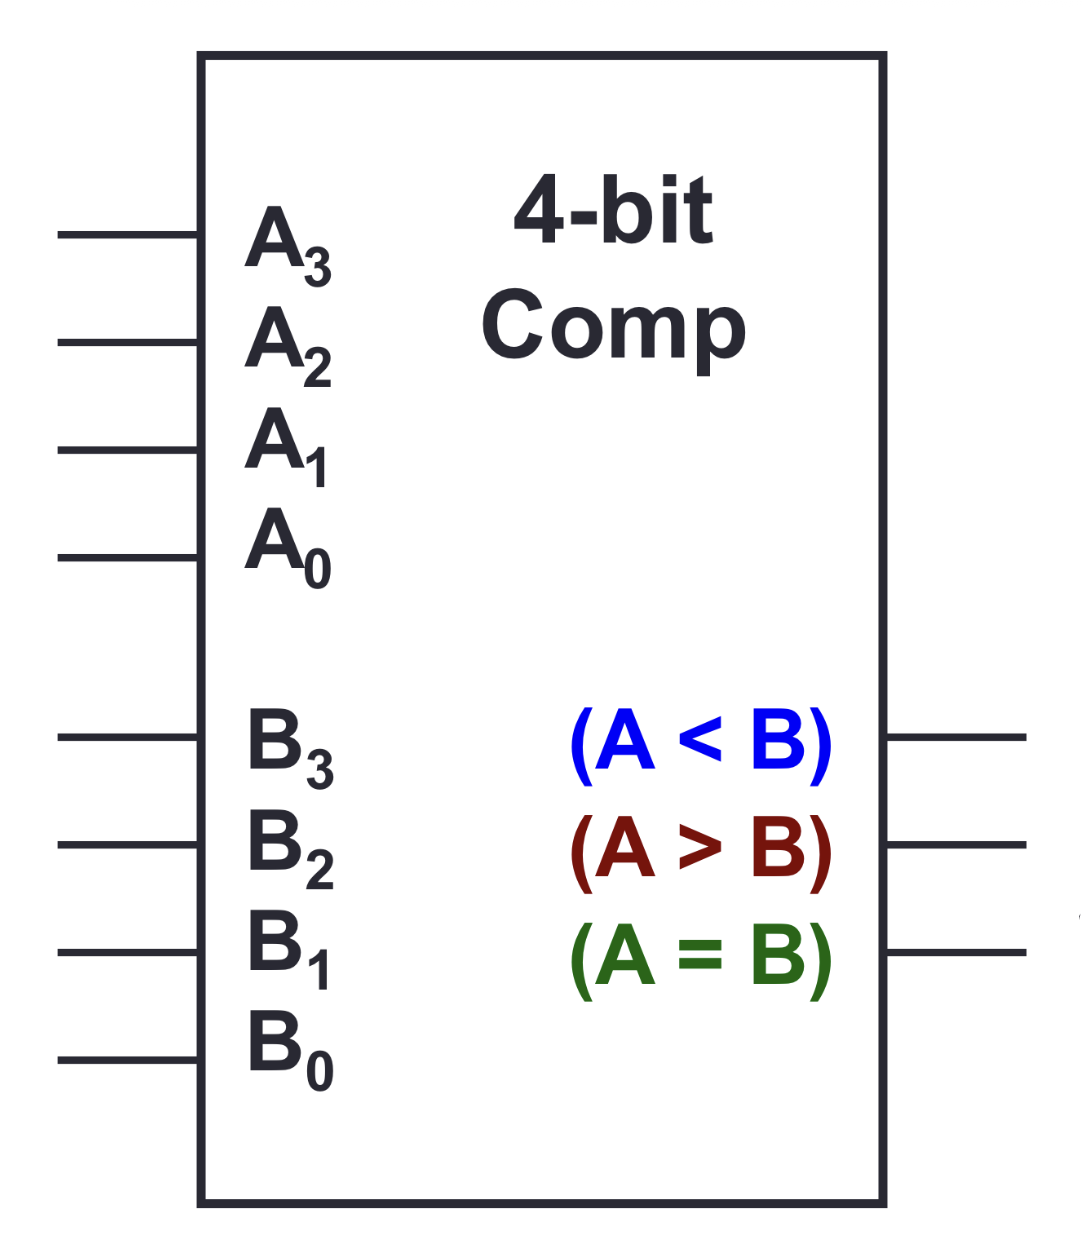
\includegraphics[height=0.3\textwidth]{compa_block}
    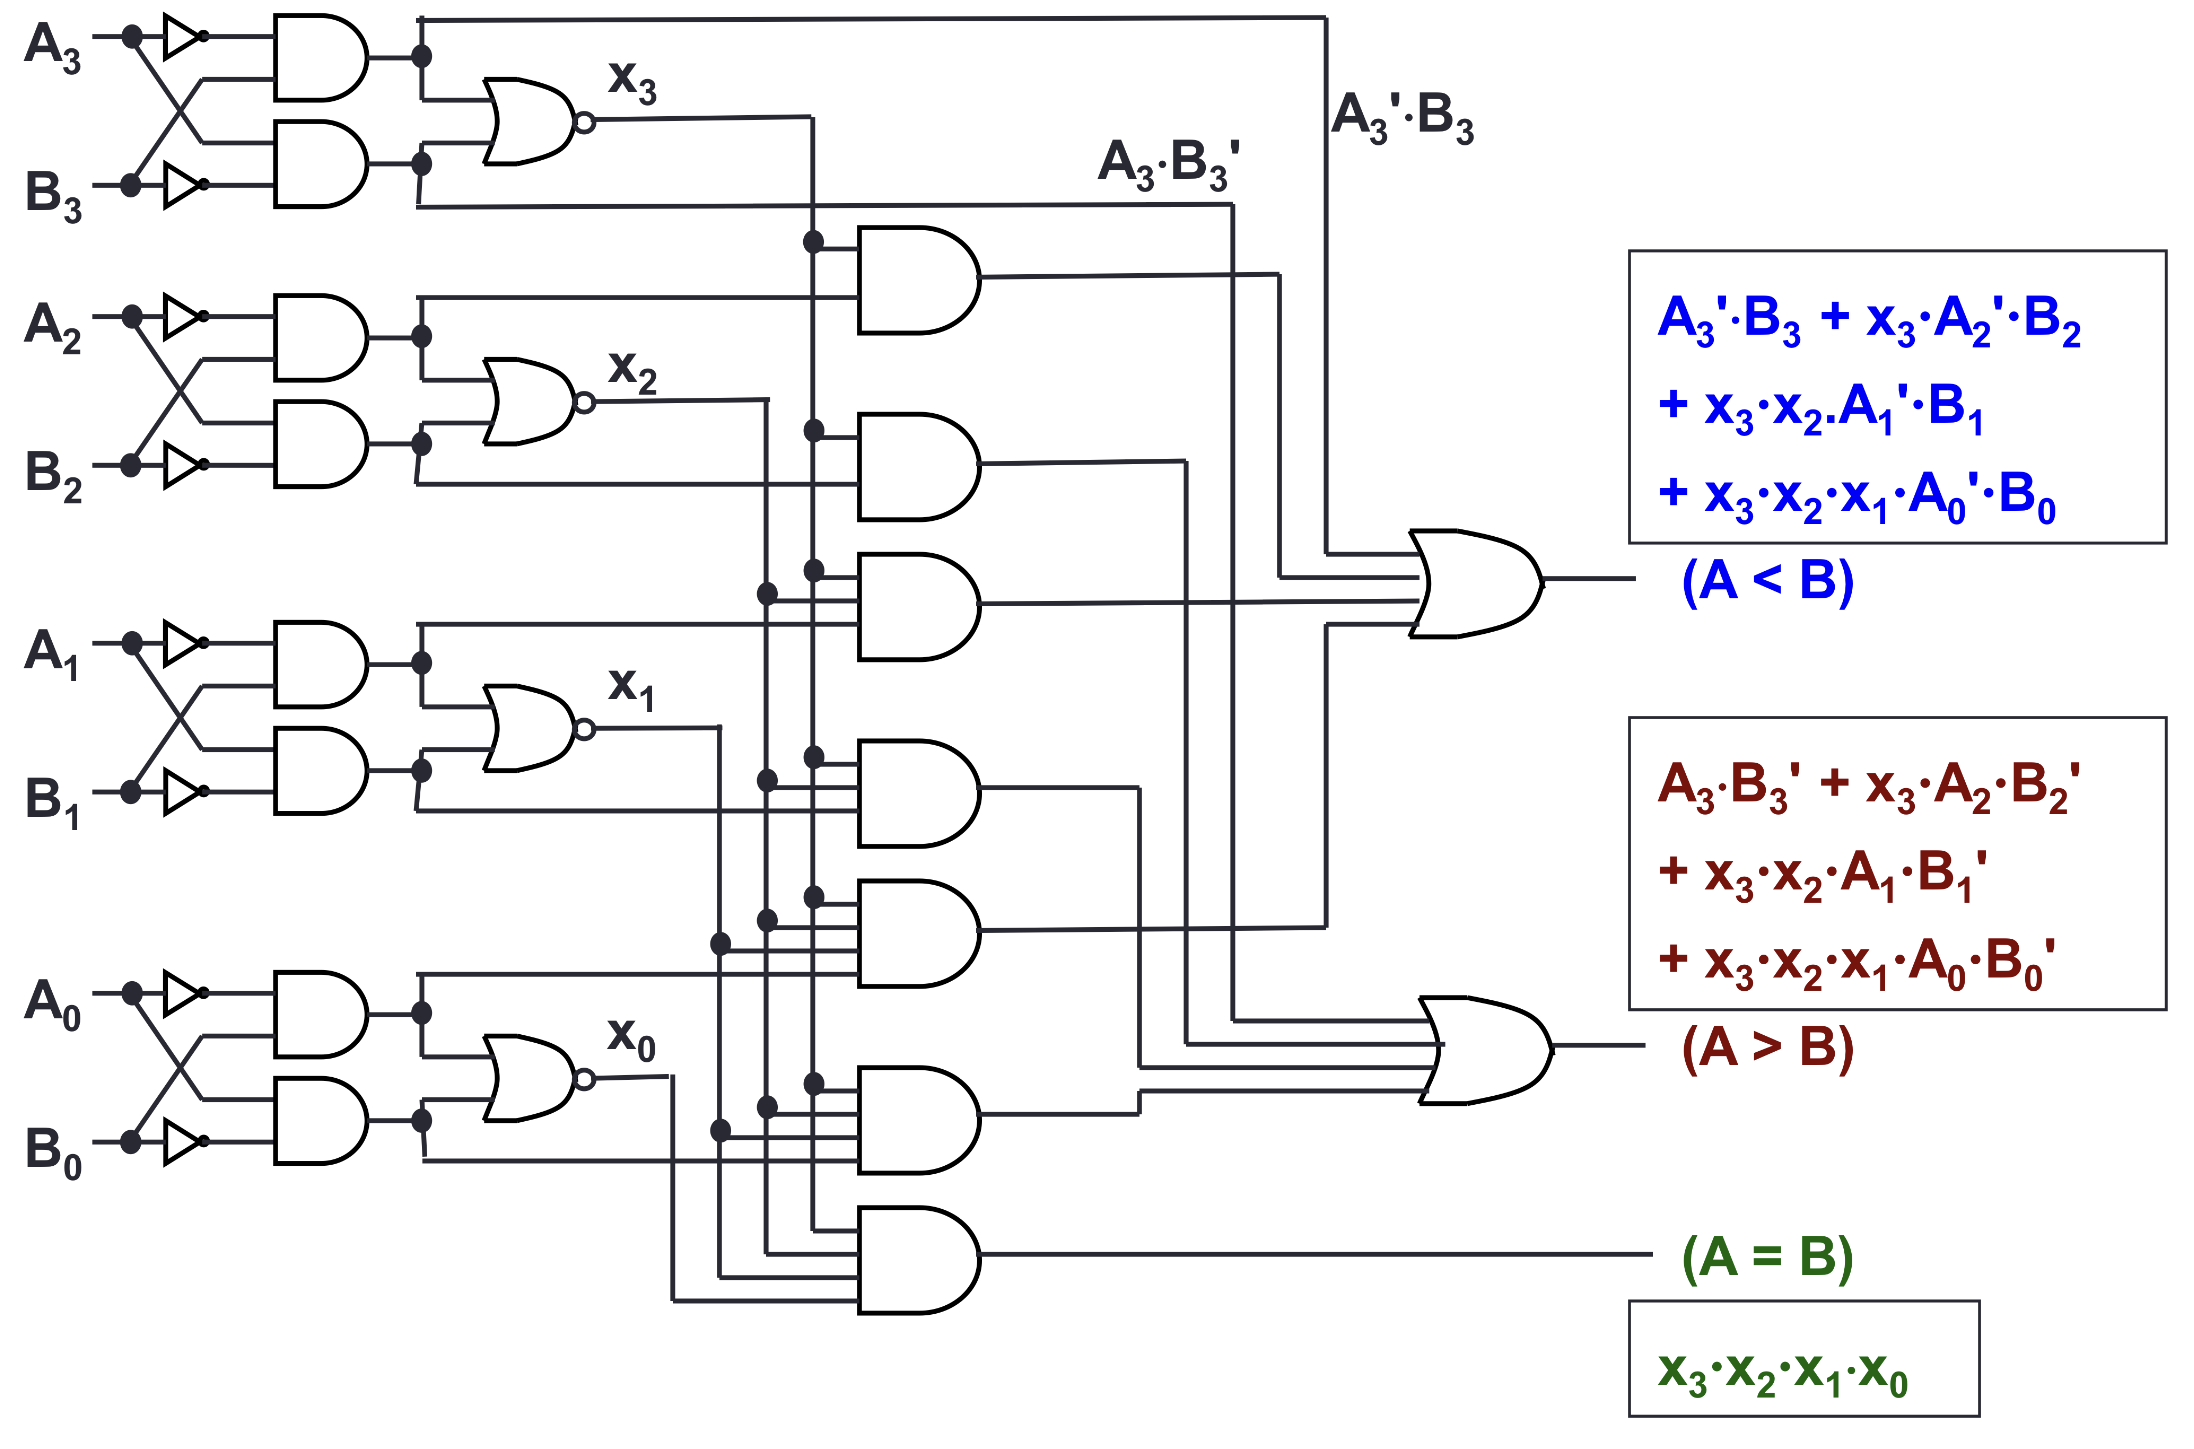
\includegraphics[height=0.3\textwidth]{compa_circuit}
  \end{figure}
\end{example}


\subsection{Sequential Circuits}
Other than combinational circuits, we now consider the class of sequential
circuits, where each output depends not only on the present inputs, but also on
the current state.

\begin{definition}[Synchronous/Asynchronous Circuits]
  \textit{Synchronous circuits} are sequential circuits where outputs change
  only at a specific time, and \textit{asynchronous circuits} are that where
  outputs change at any time.
\end{definition}

\begin{definition}[Multivibrators]
  \textit{Multivibrators} are a family of sequential circuits, within which we
  distinguish bistable (2 stable states), monostable (1 stable state) and
  astable (no stable state) circuits.
\end{definition}

\begin{definition}[Memory Elements]
  A \textit{memory element} is a device which comprises state indefinitely, or
  can change state based on its inputs.
\end{definition}

The memory elements in a sequential circuit are implemented using bistable
logic devices, namely \textbf{latches} and \textbf{flip-flops}. Memory elements
can also be controlled by a \textbf{clock}, typically a square wave consisting
positive and negative edges, and positive pulses.

\subsubsection{Latches}
Latches are memory devices that are pulse-triggered. It is ON for the duration
of positive pulses, during which it would respond to inputs for state
transitions, and preserve its state when it is OFF

\paragraph{S-R Latch}
A S-R Latch takes in two inputs $S$ (SET) and $R$ (RESET) and provides two
complementary outputs $Q$ and $Q'$. The latch is in a SET state when $Q=$HIGH
and RESET state when $Q=$LOW.

In an active-high input S-R latch, the next state is determined by the input
carrying the high signal.
\begin{figure}[h!]
  \centering
  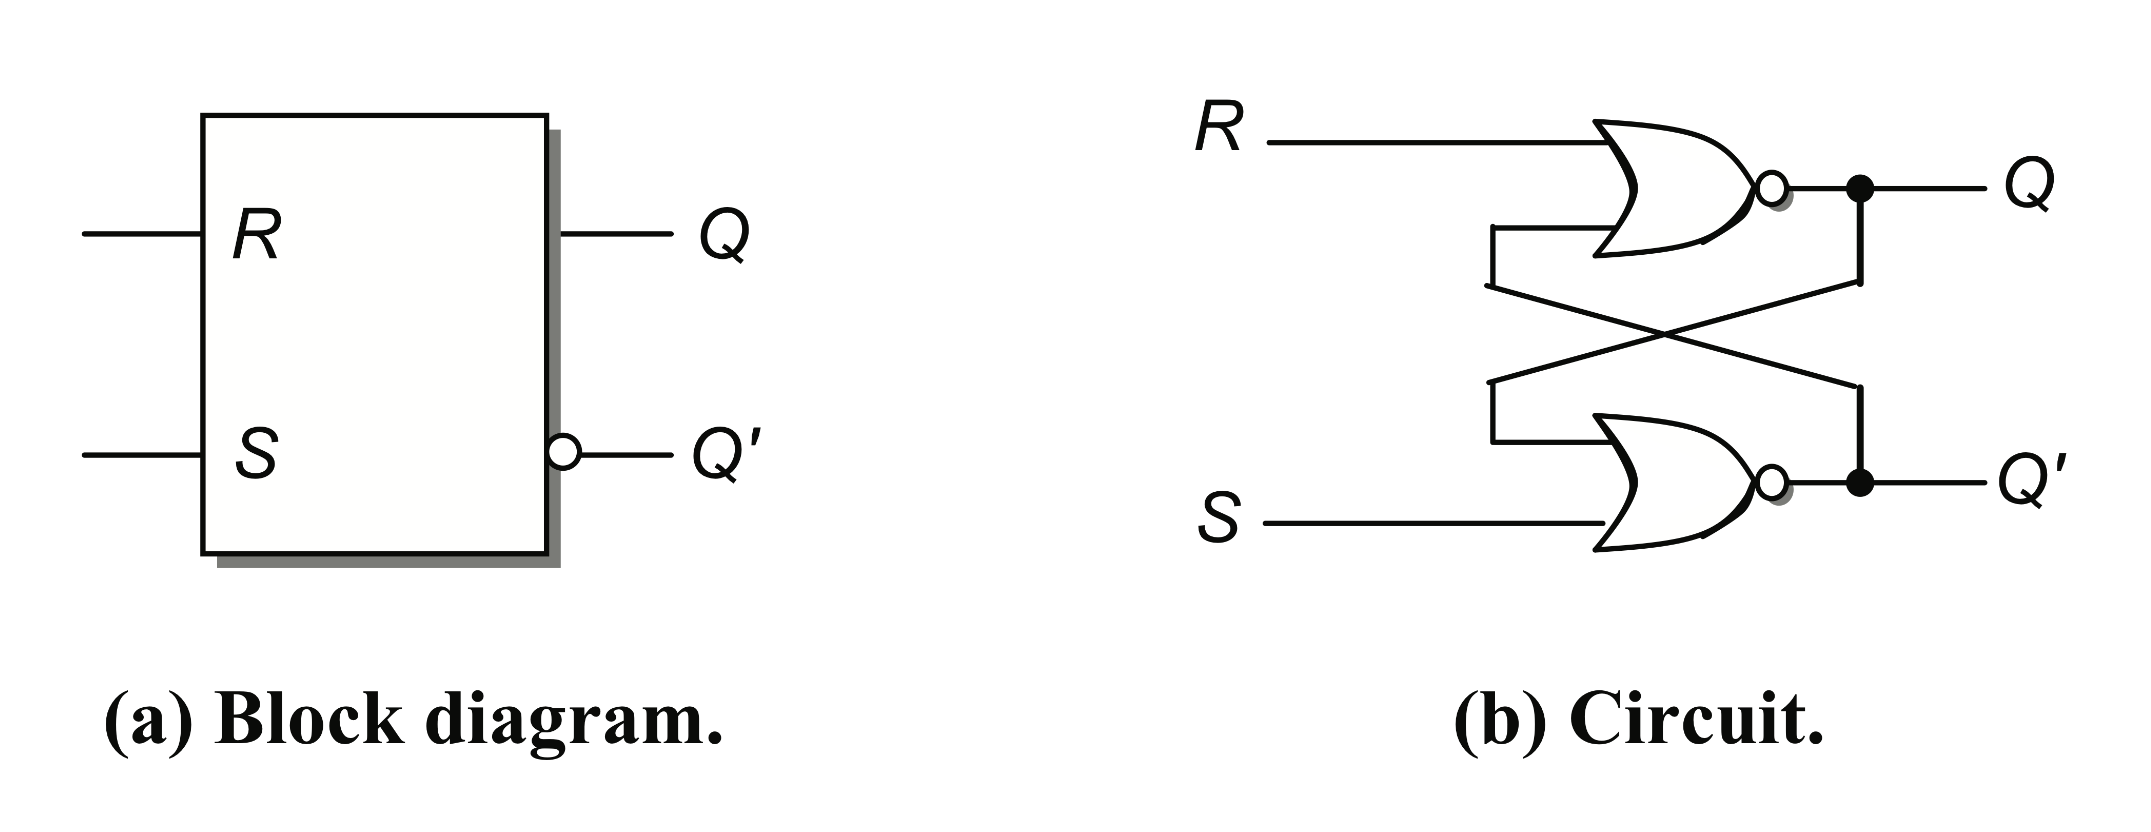
\includegraphics[width=0.4\textwidth]{sr_high}
  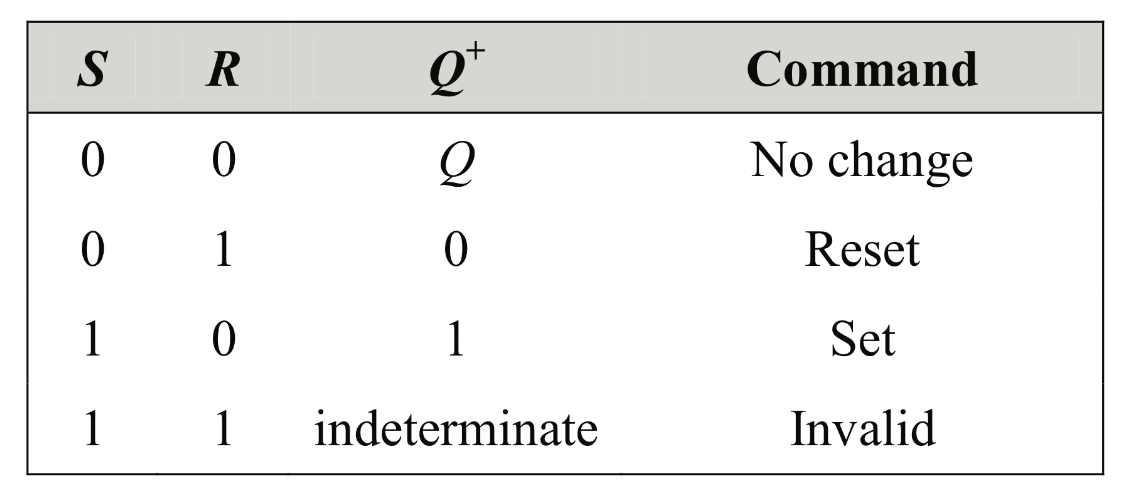
\includegraphics[width=0.35\textwidth]{sr_high_2}
\end{figure}\\
In an active-low input S-R latch, the next state is determined by the input
carrying the low signal.
\begin{figure}[h!]
  \centering
  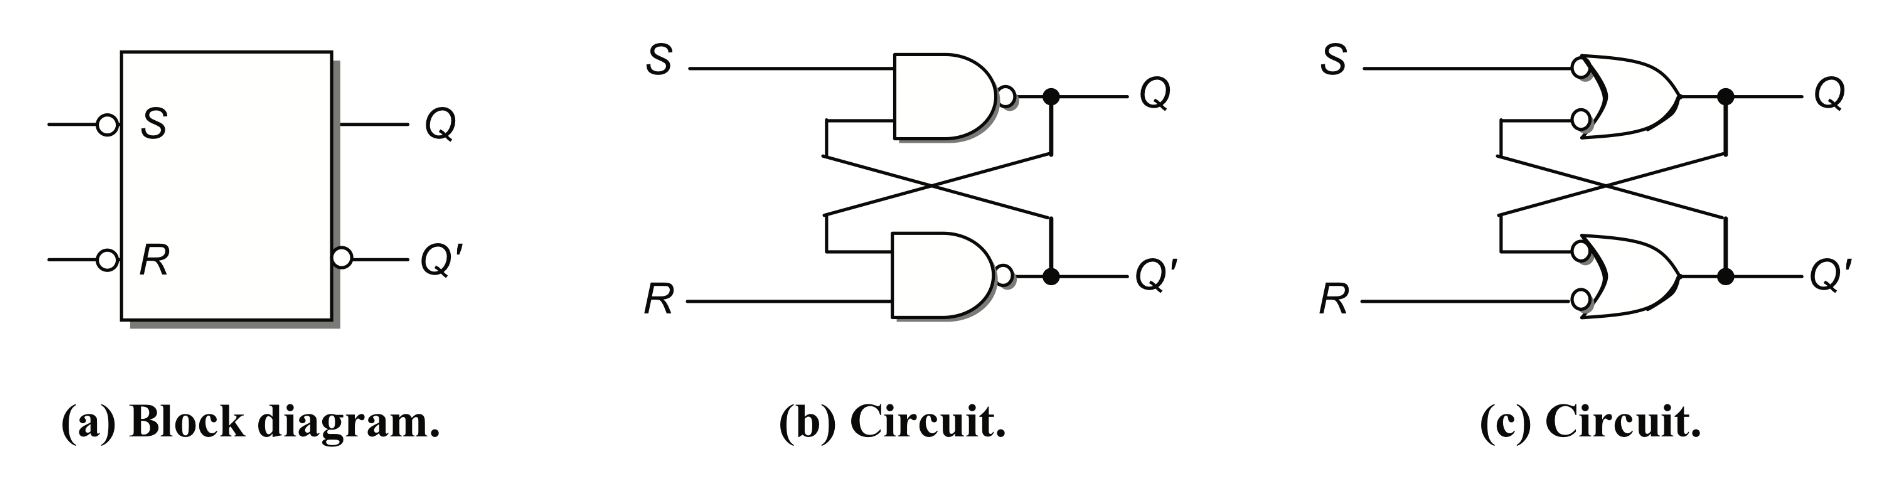
\includegraphics[width=0.5\textwidth]{sr_low}
  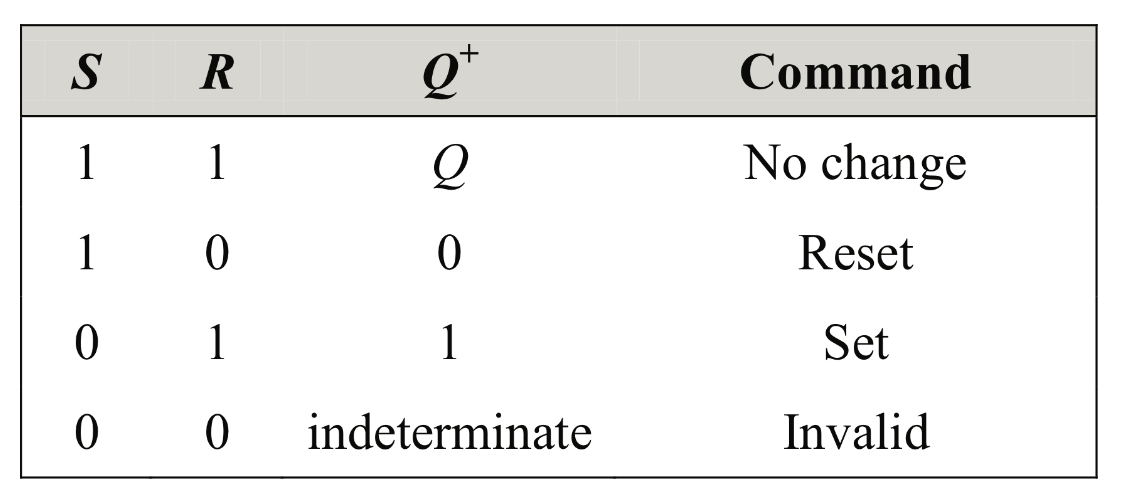
\includegraphics[width=0.35\textwidth]{sr_low_2}
\end{figure}

A pulse-triggered latch gated S-R latch is a S-R latch with an enable input.
Outputs of the latch change only if the enable input is high.
\begin{figure}[h!]
  \centering
  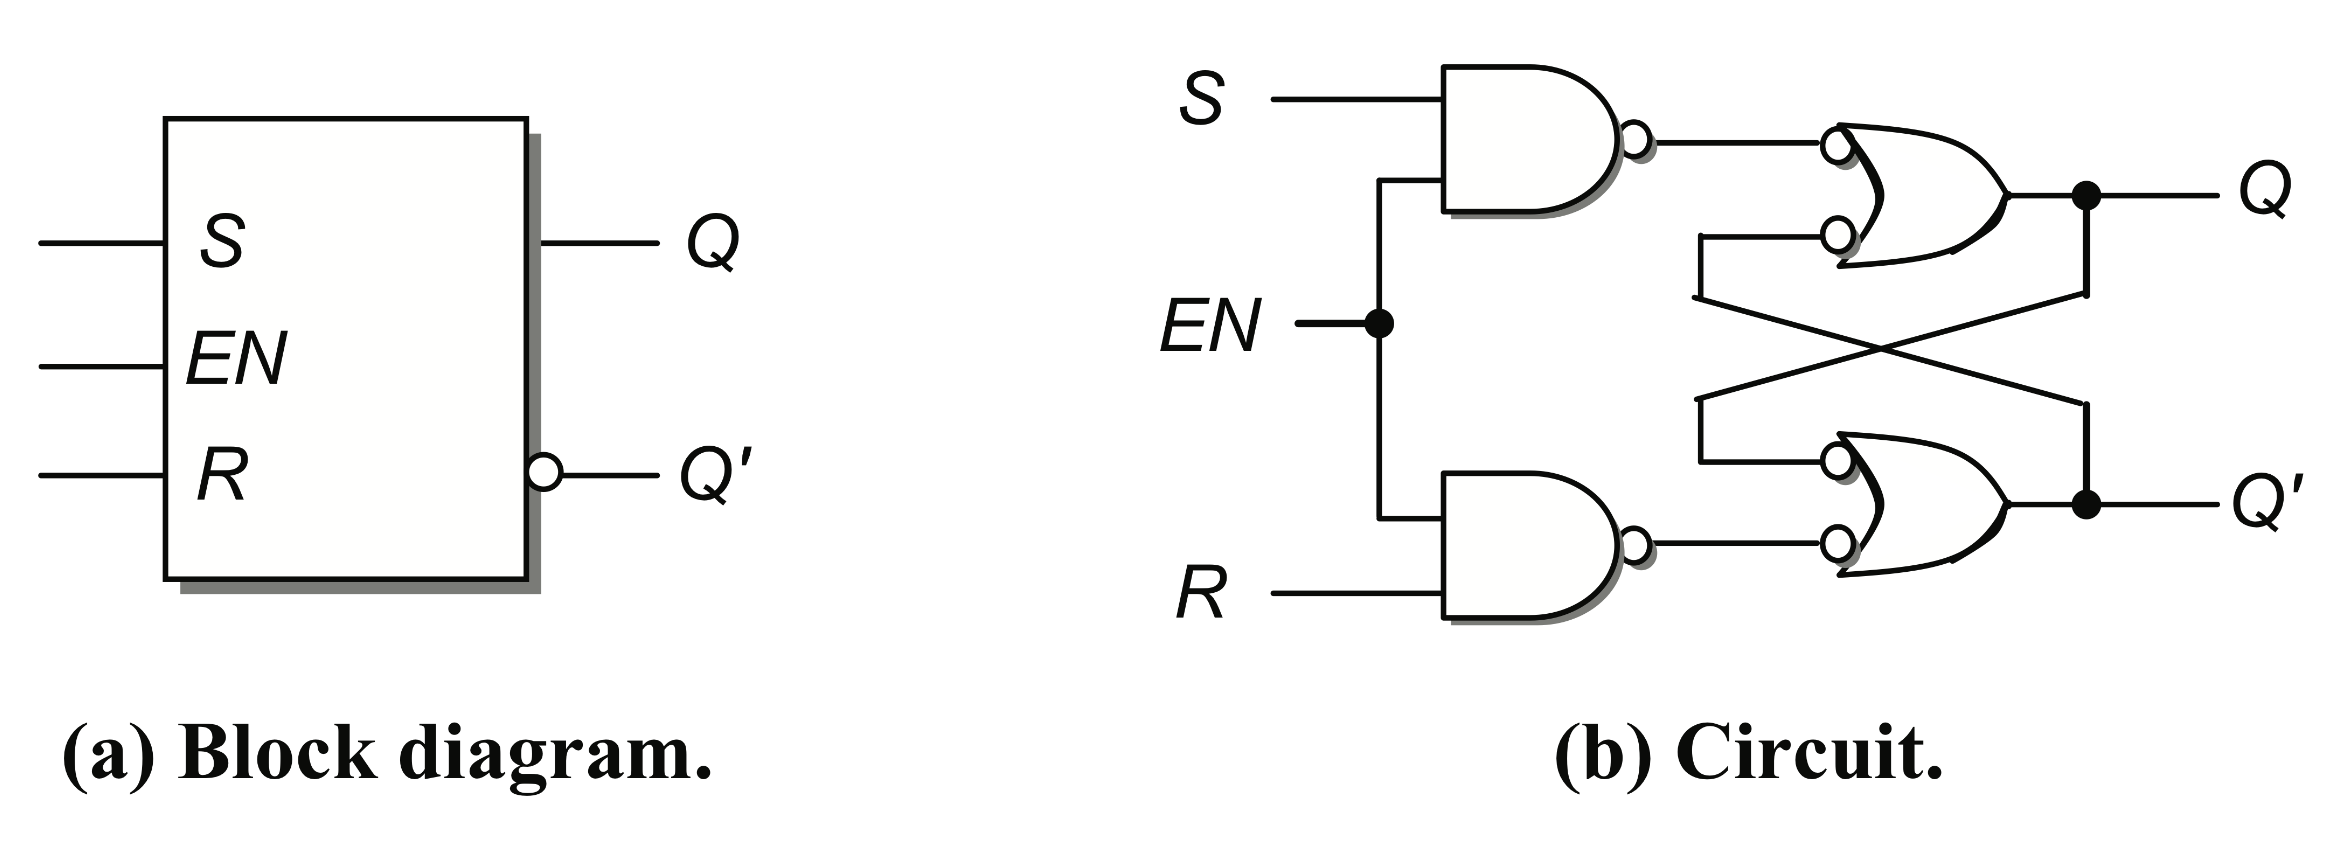
\includegraphics[width=0.4\textwidth]{sr_gated}
\end{figure}
\vspace{-4mm}
\paragraph{D Latch}
The gated D latch eliminates the invalid command in the S-R latch by
constraining the inputs for an S-R latch to be $D$ and $D'$.
\begin{figure}[h!]
  \centering
  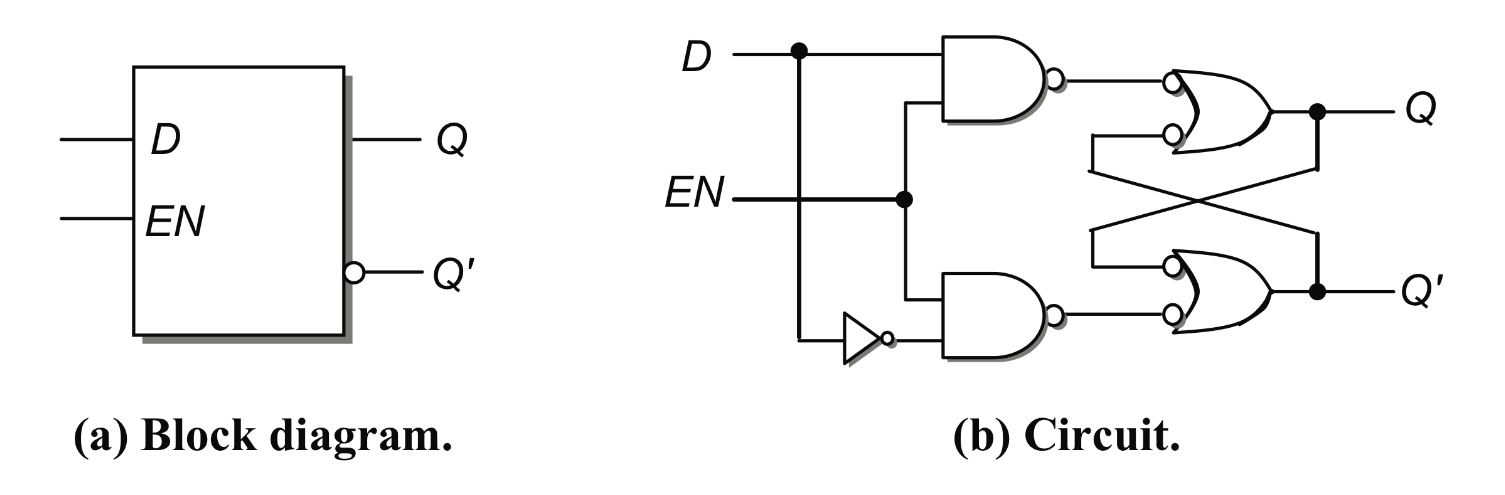
\includegraphics[width=0.4\textwidth]{d_gated}
  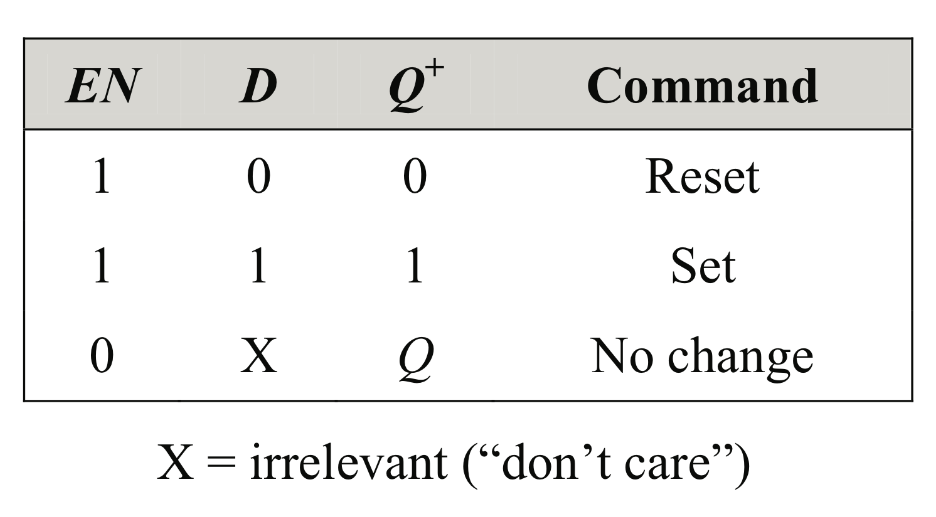
\includegraphics[width=0.3\textwidth]{d_gated_2}
\end{figure}
\vspace{-4mm}
\subsubsection{Flip-Flops}
Flip-flops are synchronous bistable memory devices that are edge-triggered.
That is, state is updated at a specified point on the clock signal, either at
the positive (rising) edge, or at the negative (falling) edge.
\begin{figure}[h!]
  \centering
  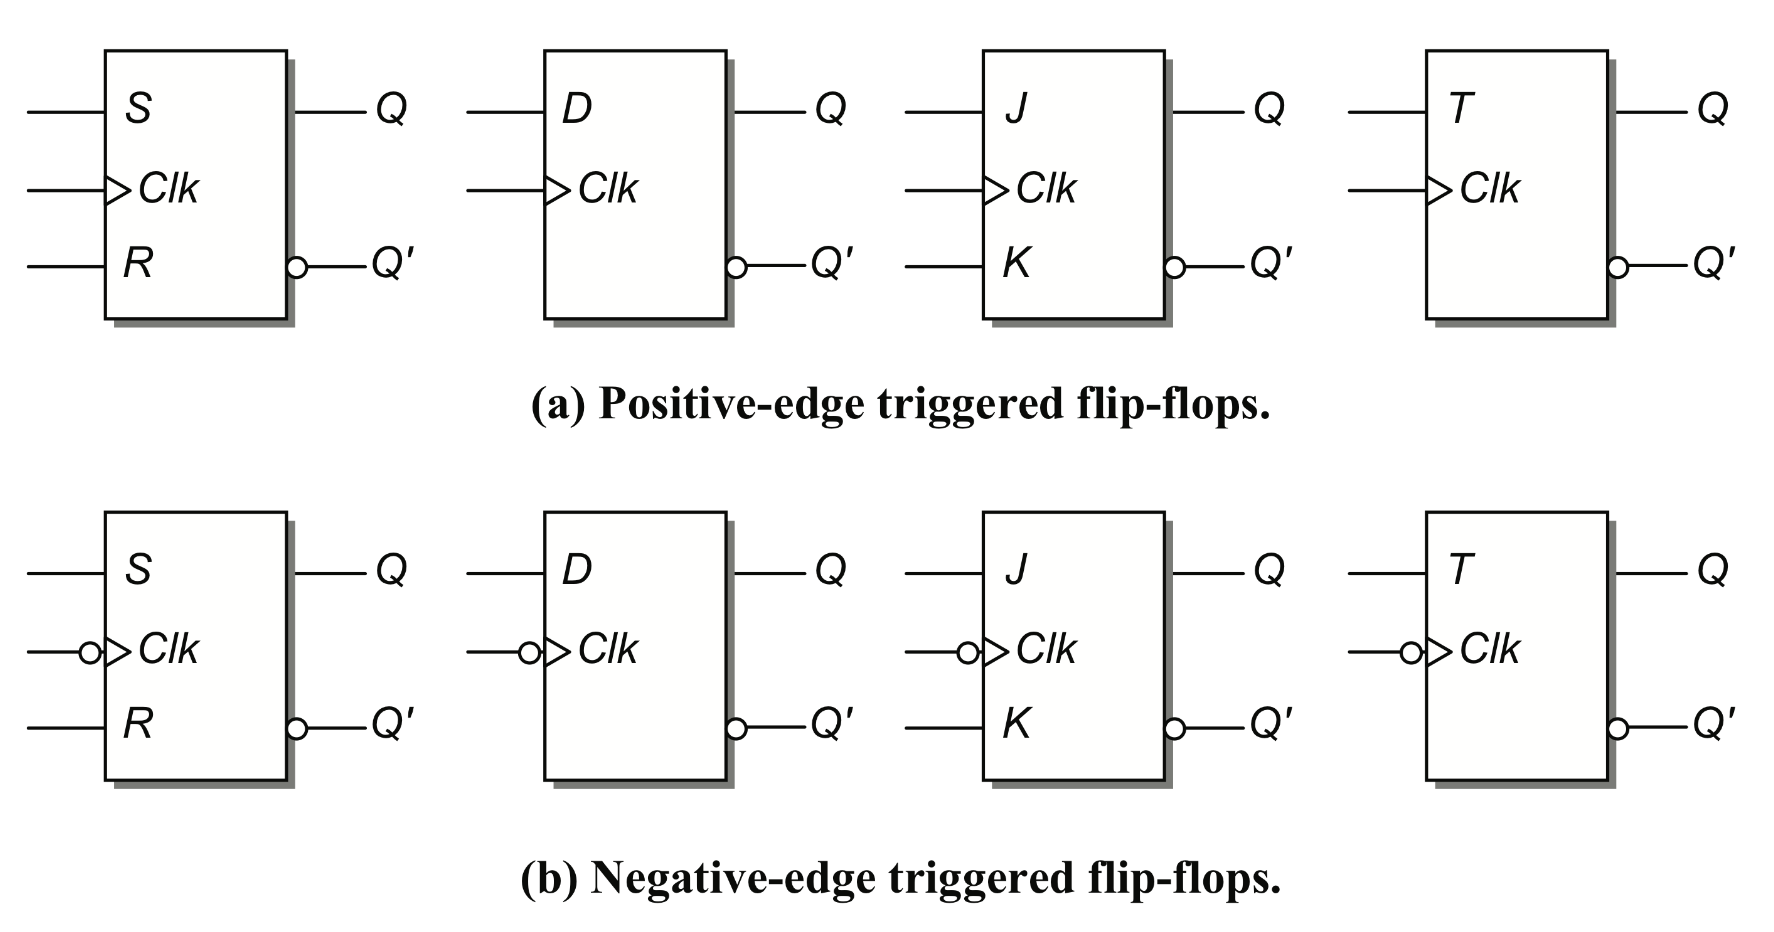
\includegraphics[width=0.65\textwidth]{flipflops}
\end{figure}
\vspace{-8mm}
\paragraph{S-R Flip-Flop} A positive-edge triggered S-R Flip-Flop behaves as a
synchronous version of an active-high input S-R latch. $Q^{+}=S+R'\cdot Q$ where $S\cdot R=0$.
\begin{figure}[h!]
  \centering
  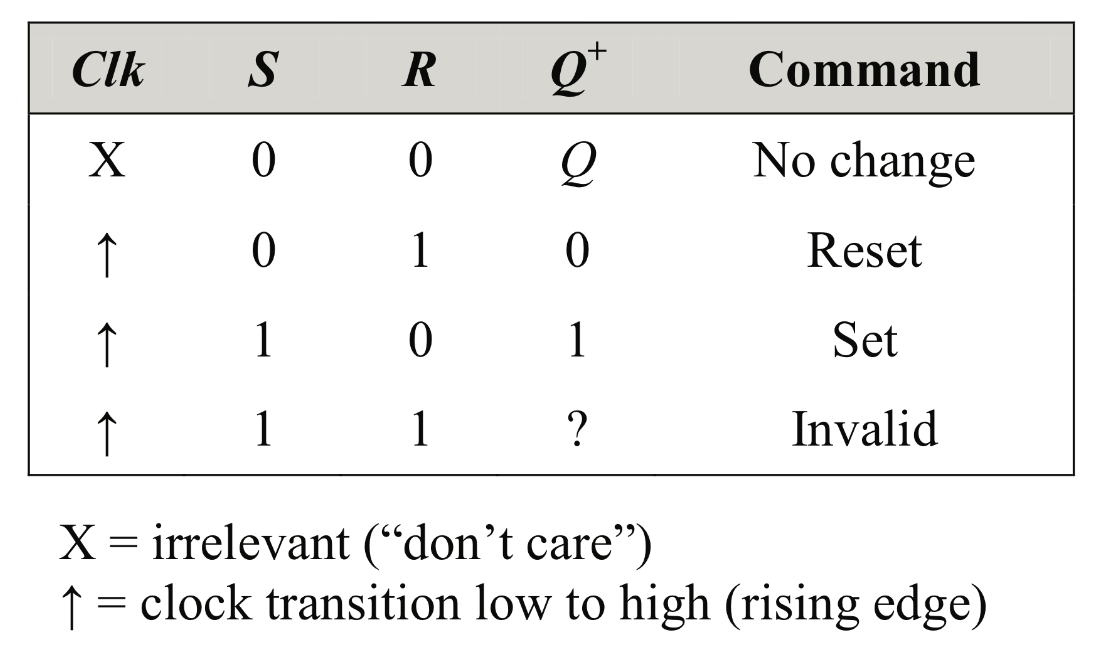
\includegraphics[width=0.38\textwidth]{srff}
\end{figure}
\vspace{-8mm}
\paragraph{D Flip-Flop} A positive-edge triggered D flip-flop behaves as a
synchronous version of an active-high input D latch. $Q^{+}=D$.
\begin{figure}[h!]
  \centering
  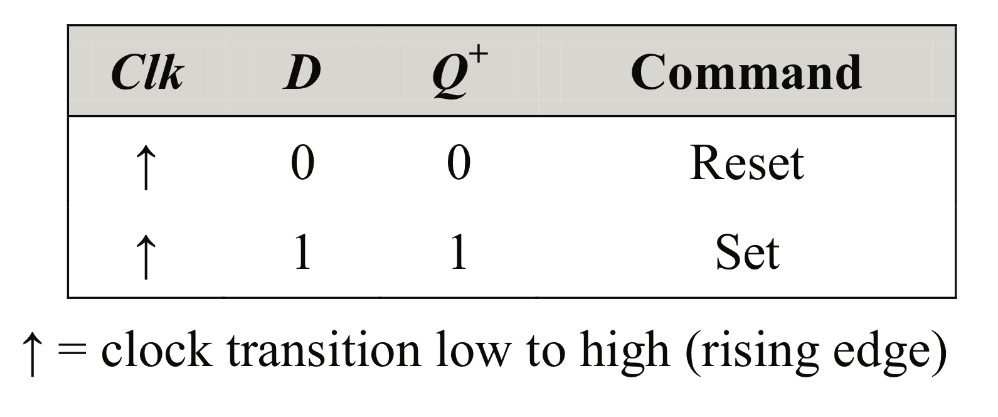
\includegraphics[width=0.35\textwidth]{dff}
\end{figure}
\vspace{-8mm}
\paragraph{J-K Flip-Flop} In a J-K flip-flop, $Q$ and $Q'$ are fed back to the
pulse-steering NAND gates. We eliminate the invalid state, which becomes a toggle
state. $Q^{+}=J\cdot Q'+K'\cdot Q$.
\begin{figure}[h!]
  \centering
  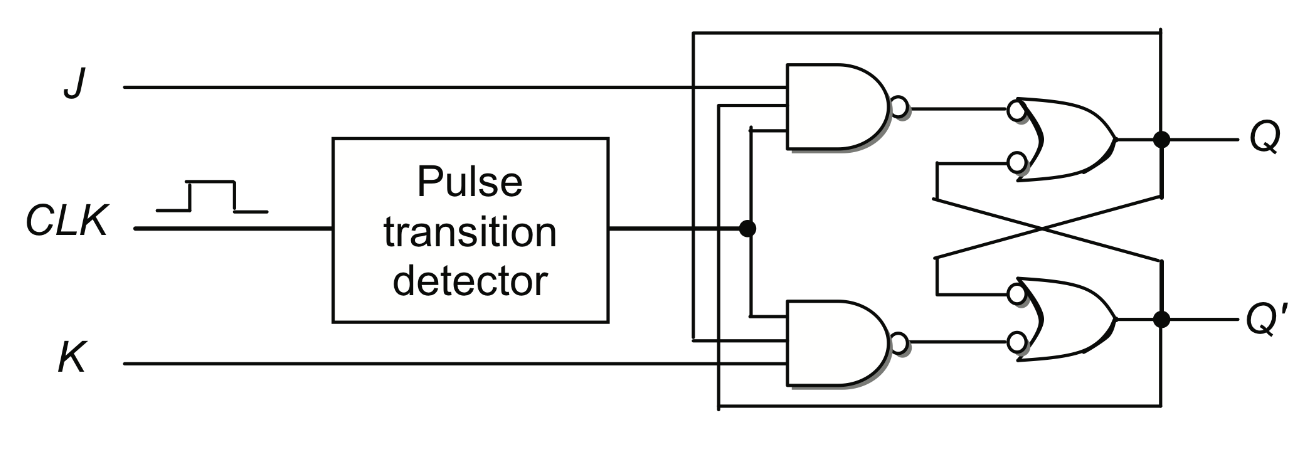
\includegraphics[width=0.4\textwidth]{jkff}
  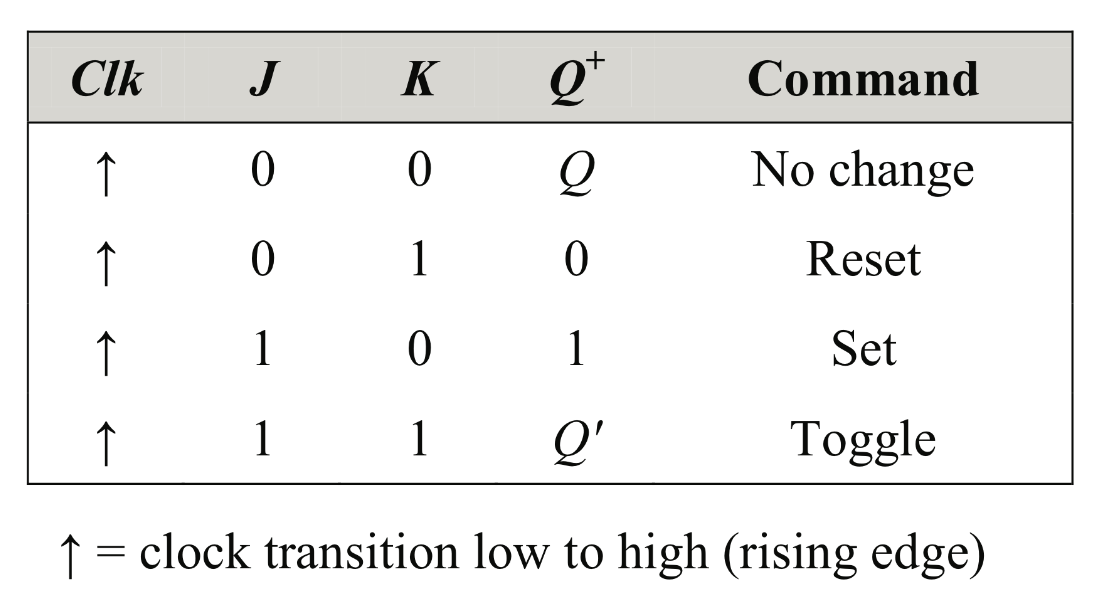
\includegraphics[width=0.38\textwidth]{jkff2}
\end{figure}
\vspace{-8mm}
\paragraph{T Flip-Flop} The T flip-flop is a single input version of the J-K
flip-flop where $J=K=T$, which triggers the toggle state. $Q^{+}=T\cdot Q'+T'\cdot Q$.
\begin{figure}[h!]
  \centering
  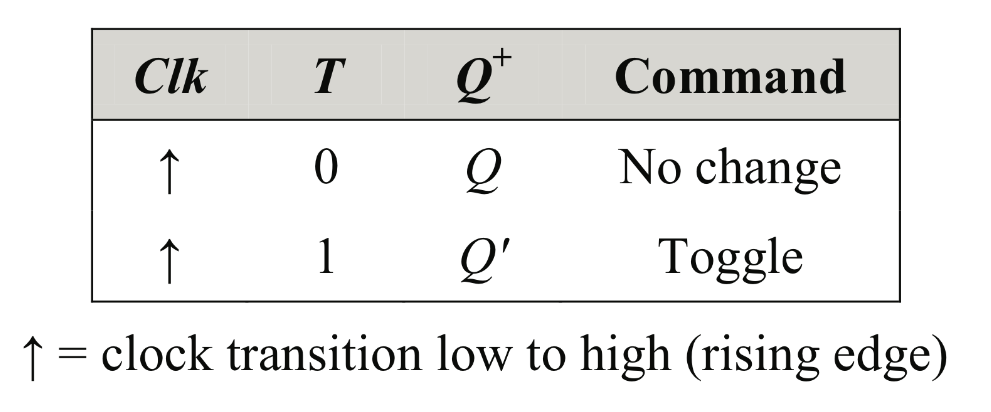
\includegraphics[width=0.35\textwidth]{tff}
\end{figure}
\vspace{-4mm}
\begin{definition}[Synchronous/Asynchronous Inputs]
  A \textit{synchronous input} is one where data is transferred to the output
  only at a specific time, and an \textit{asynchronous input} is one that
  affects the state independent of the clock.
\end{definition}
\begin{example}[Flip-Flops]
  For the flip-flops, we have the synchronous inputs $S$-$R$, $D$, and $J$-$K$.
  We may also have the asynchronous inputs $PRE$ or $SD$ (Preset/Direct Set),
  $CLR$ or $RD$ (Clear/Direct Reset). When $PRE=$HIGH, $Q=$HIGH
  \textit{immediately} and when $CLR=$HIGH, $Q=$LOW \textit{immediately}.
  \begin{figure}[h!]
    \centering
    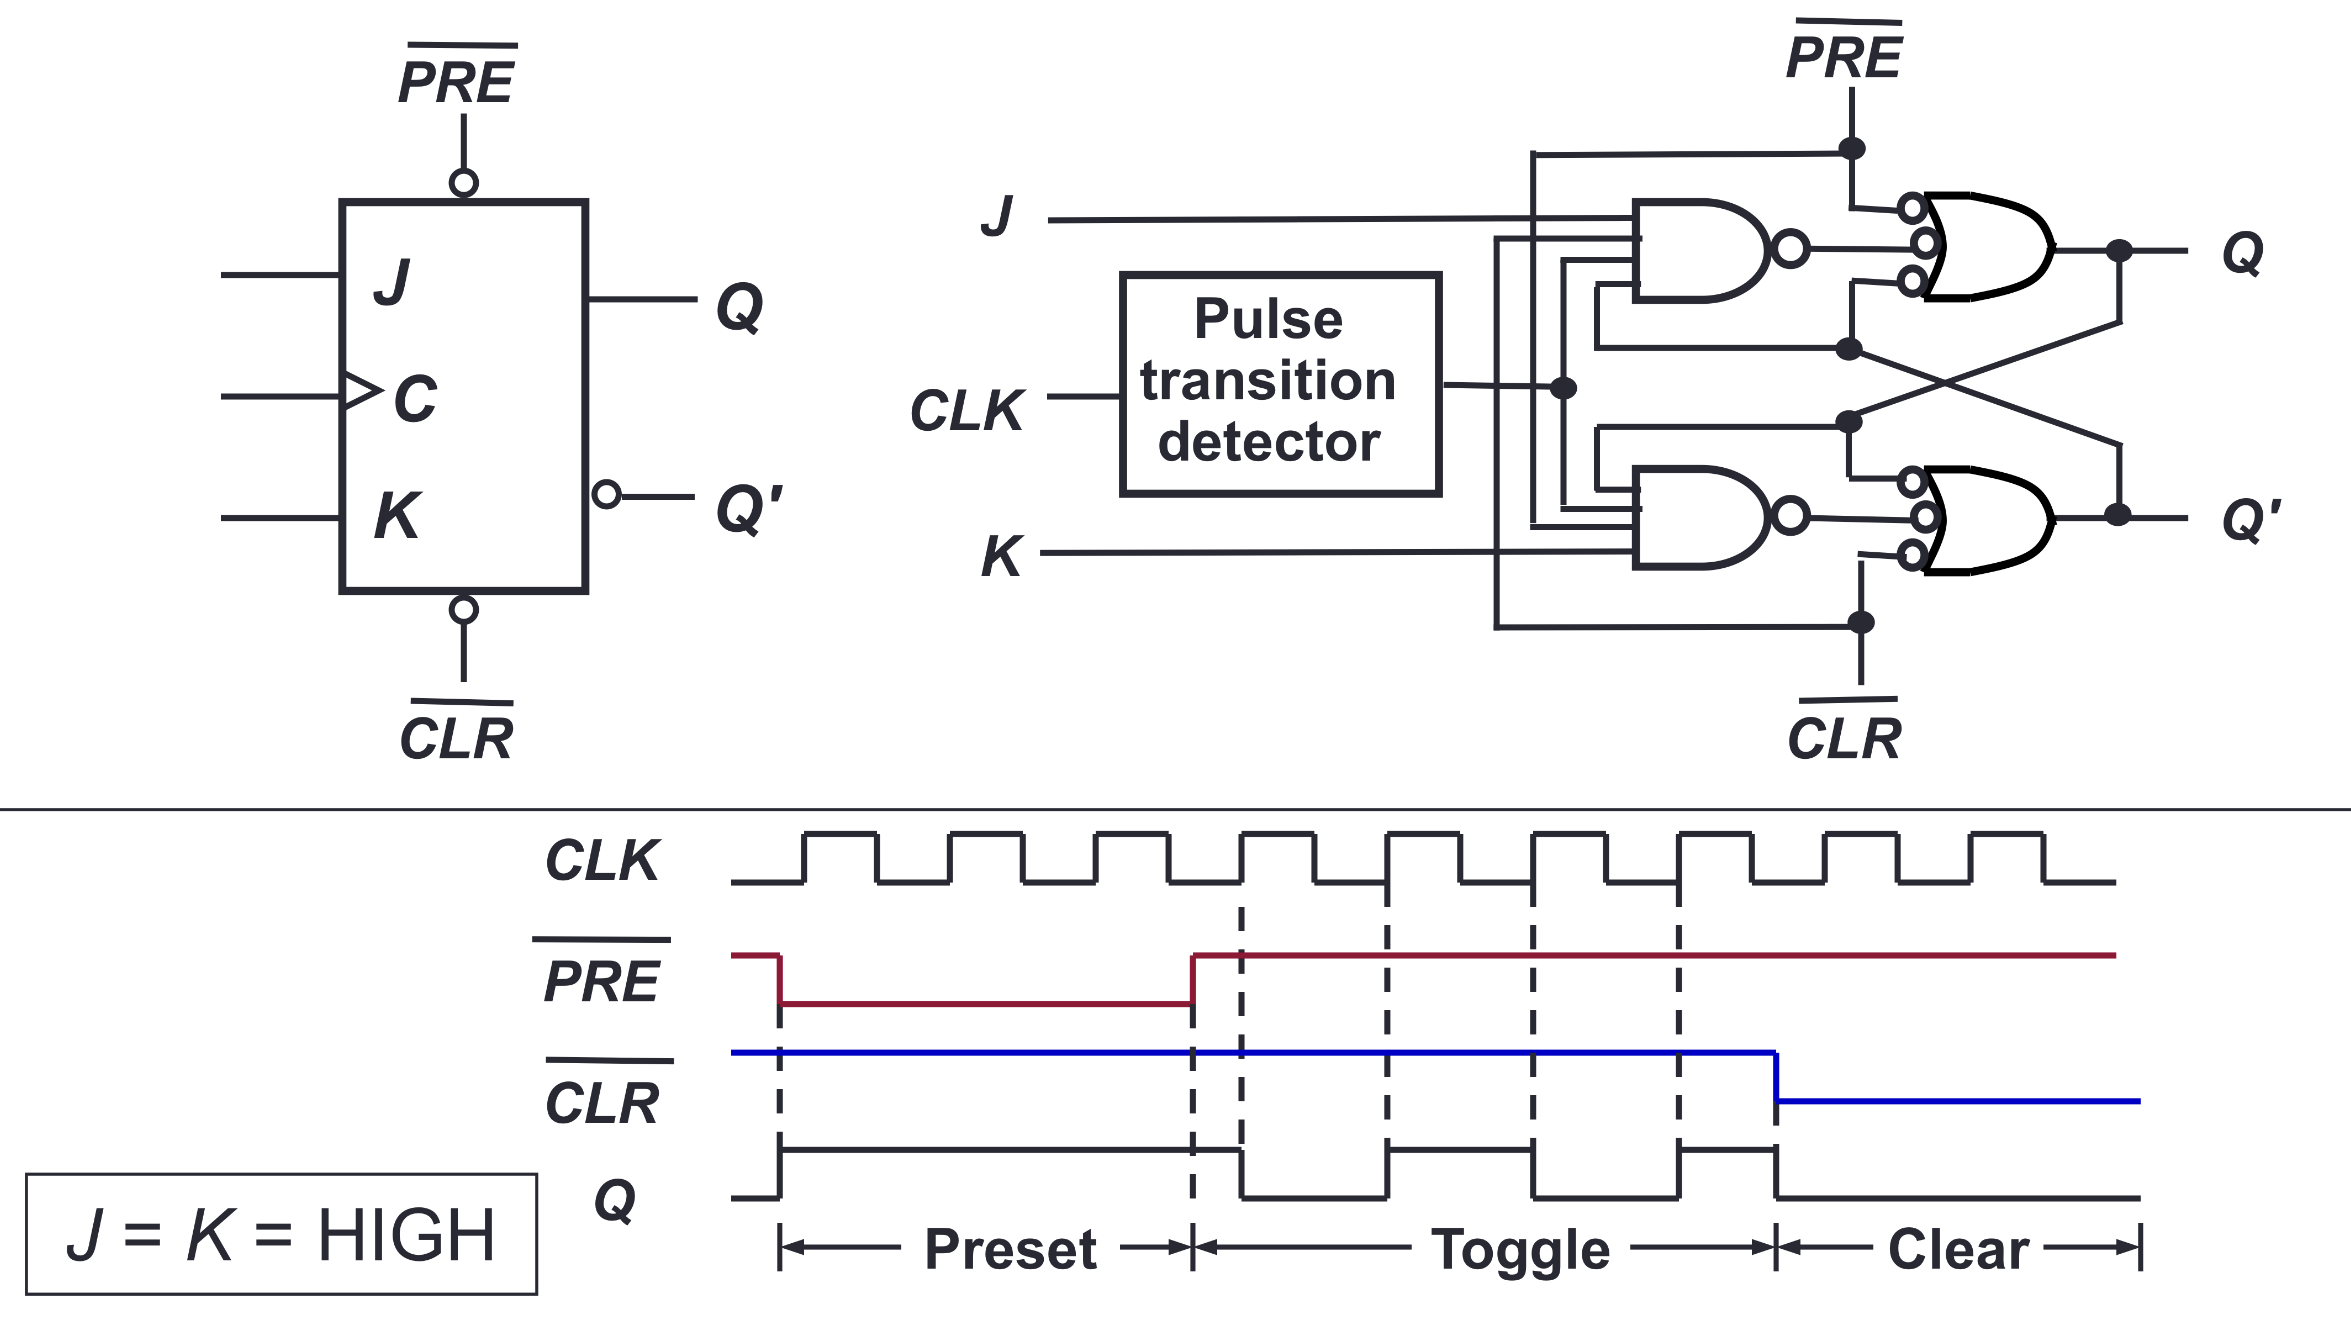
\includegraphics[width=0.55\textwidth]{async_ff}
  \end{figure}
\end{example}

\subsubsection{Sequential Circuit Analysis}
Given a sequential circuit, we analyse its behaviour by deriving its state
table and state diagram. We do so with the following procedure:
\begin{enumerate}
  \item Derive flip-flop input functions for each flip-flop. We denote each
    flip-flop input with two letters, the input's name and the flip-flop's
    name. We algebraically describe the inputs to the flip-flops.
  \item Using the characteristic tables, obtain state equations for each
    flip-flop.
  \item Derive output functions for each non-flip-flop output of the circuit.
  \item Draw and fill the state table consisting all possible binary
    combinations of present states and inputs, to show the outputs and next
    state. This consists $2^{m+n}$ rows for $m$ flip-flops and $n$-inputs.
  \item The state table can be optionally drawn more compactly by representing
    the current state of multiple variables in a single column.
  \item Derive the state diagram, where each of the $2^{m}$ node denotes a
    state, an arrow denotes a transition of state and a label of the form $a/b$
    is attached to an arrow where $a$ denotes the inputs and $b$ the outputs of
    the circuit in that transition.
\end{enumerate}
\begin{example}[Sequential Circuit Analysis]
  \begin{figure}[h!]
    \centering
    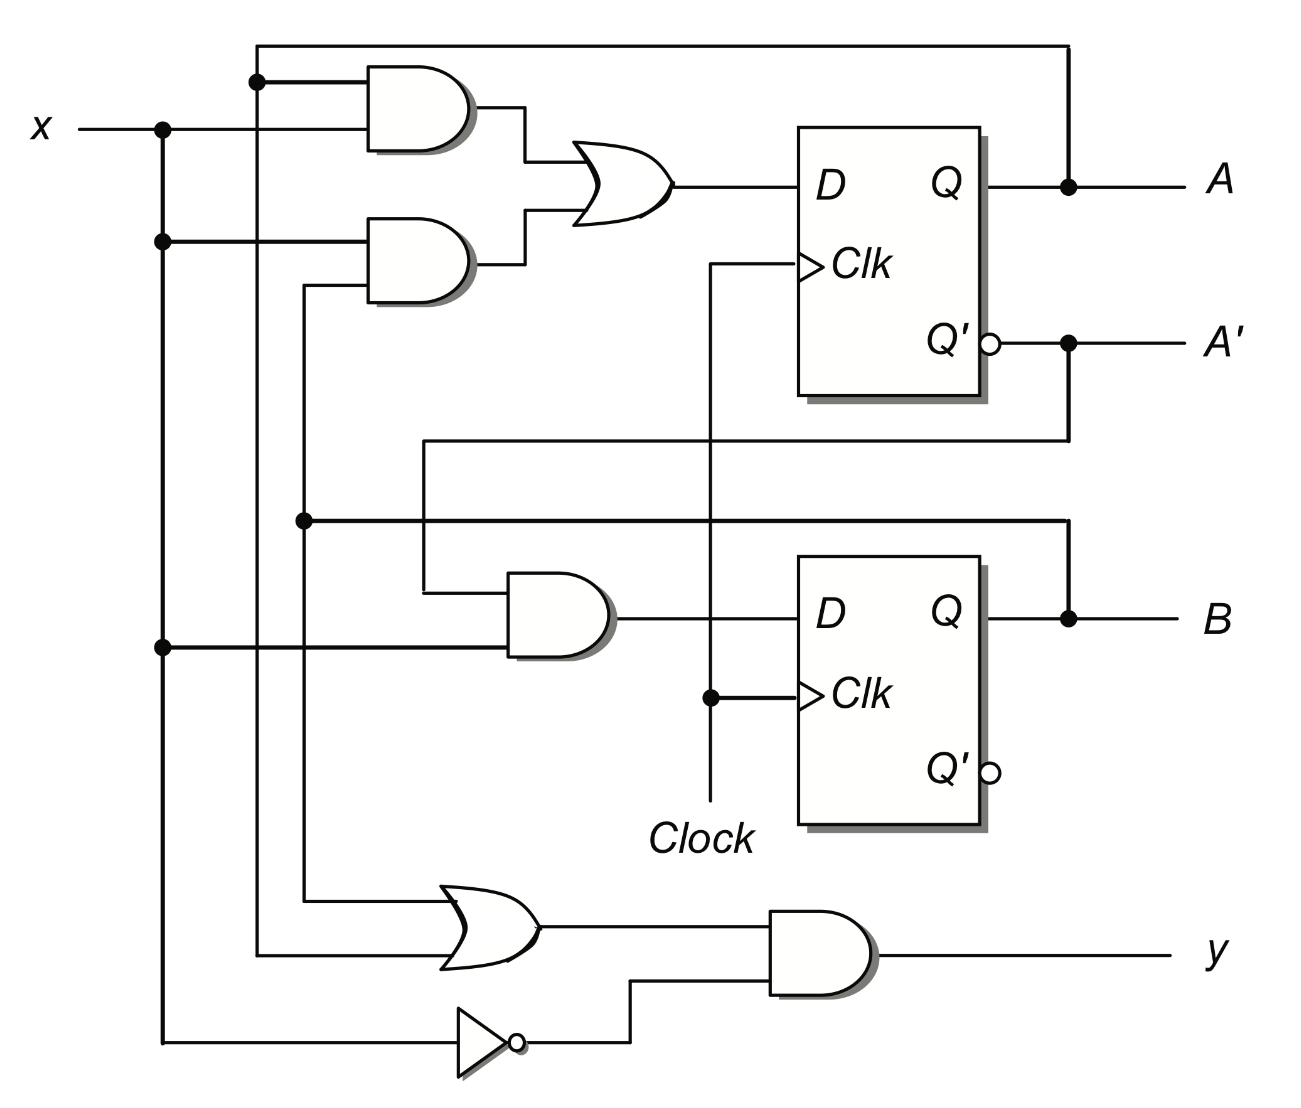
\includegraphics[width=0.4\textwidth]{seq_an}
  \end{figure}
  With the given sequential circuit, we obtain the flip-flop input functions
  for flip-flops $A$ and $B$:
  \[DA=A\cdot x+B\cdot x,\qquad DB=A'\cdot x.\] 
  Using the characteristic table of the $D$ flip-flop, we hence have the state
  equations and output function of $y$
  \[A^{+}=A\cdot x+B\cdot x,\qquad B^{+}=A'\cdot x,\qquad y=\left( A+B \right)
  \cdot x'.\]
  With these equations and functions, we obtain the state tables and diagram of
  the circuit.
  \begin{figure}[h!]
    \centering
    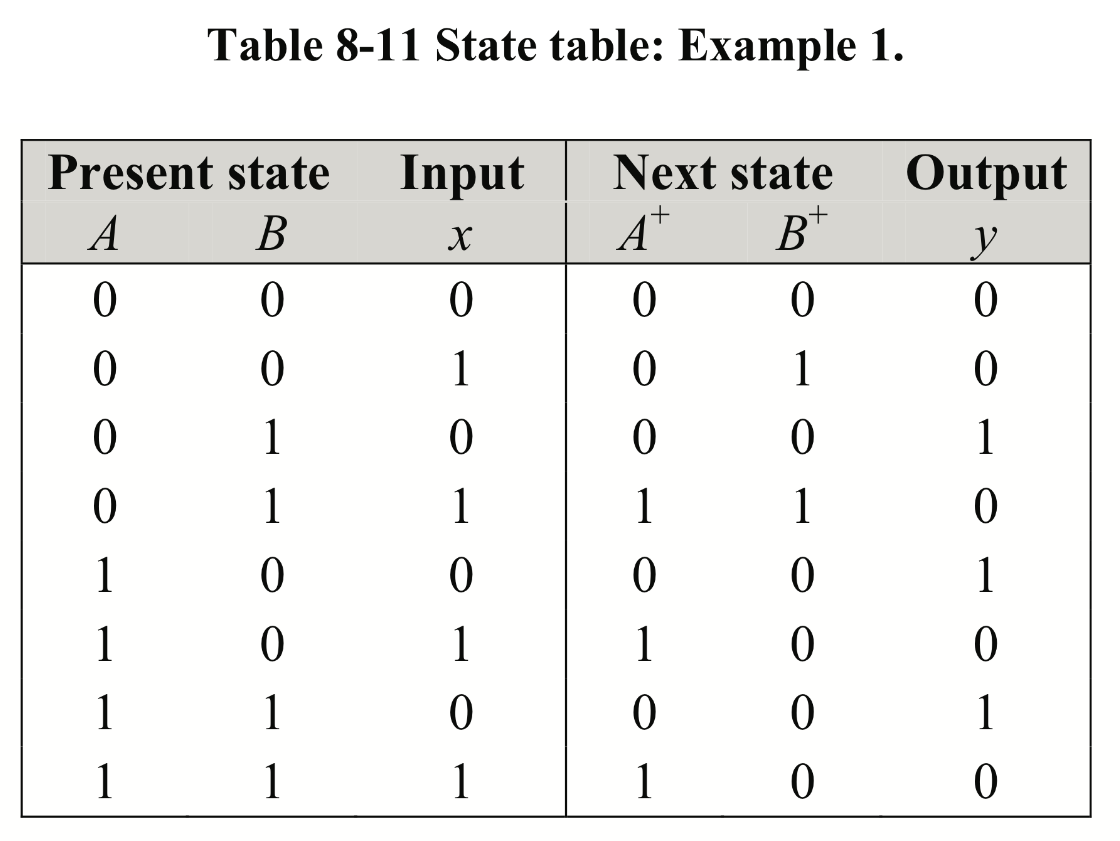
\includegraphics[width=0.33\textwidth]{seq_an1}
    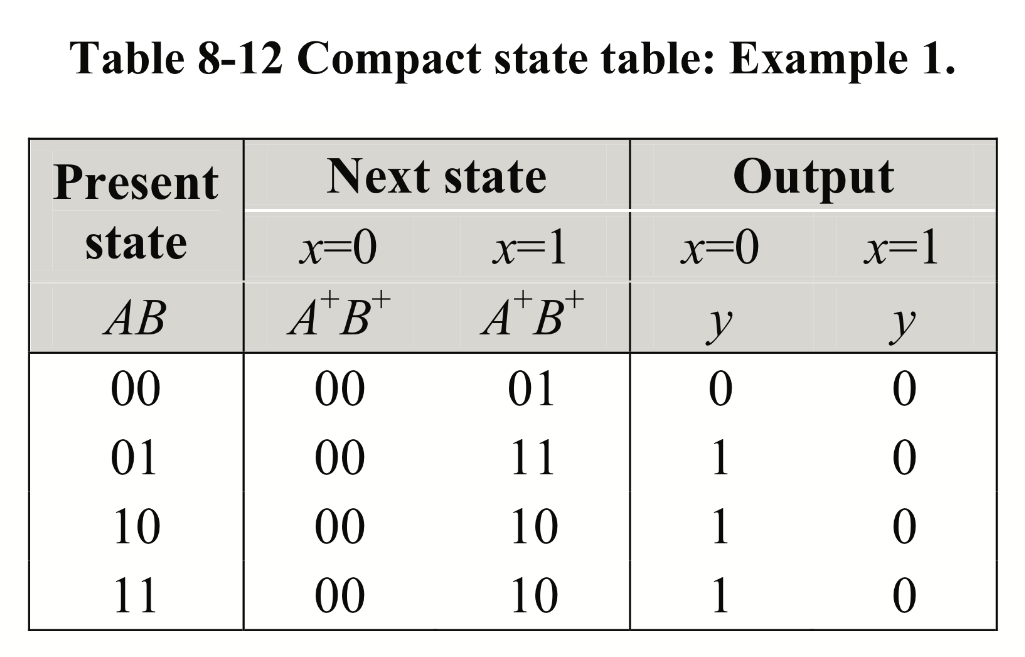
\includegraphics[width=0.3\textwidth]{seq_an2}
    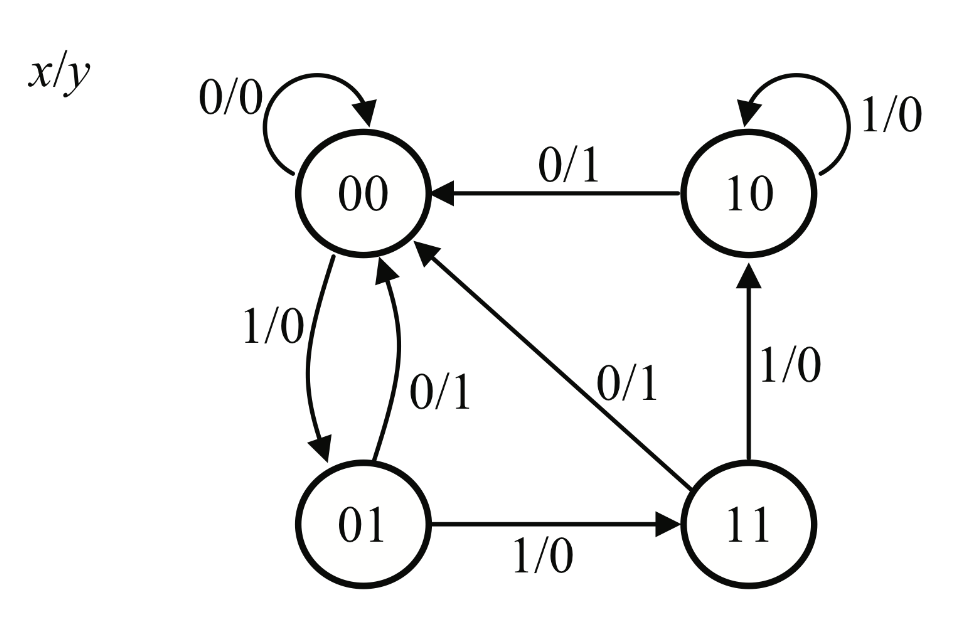
\includegraphics[width=0.33\textwidth]{seq_an3}
  \end{figure}
\end{example}
\vspace{-8mm}
\subsubsection{Sequential Circuit Design}
\vspace{-4mm}
\begin{figure}[h!]
  \centering
  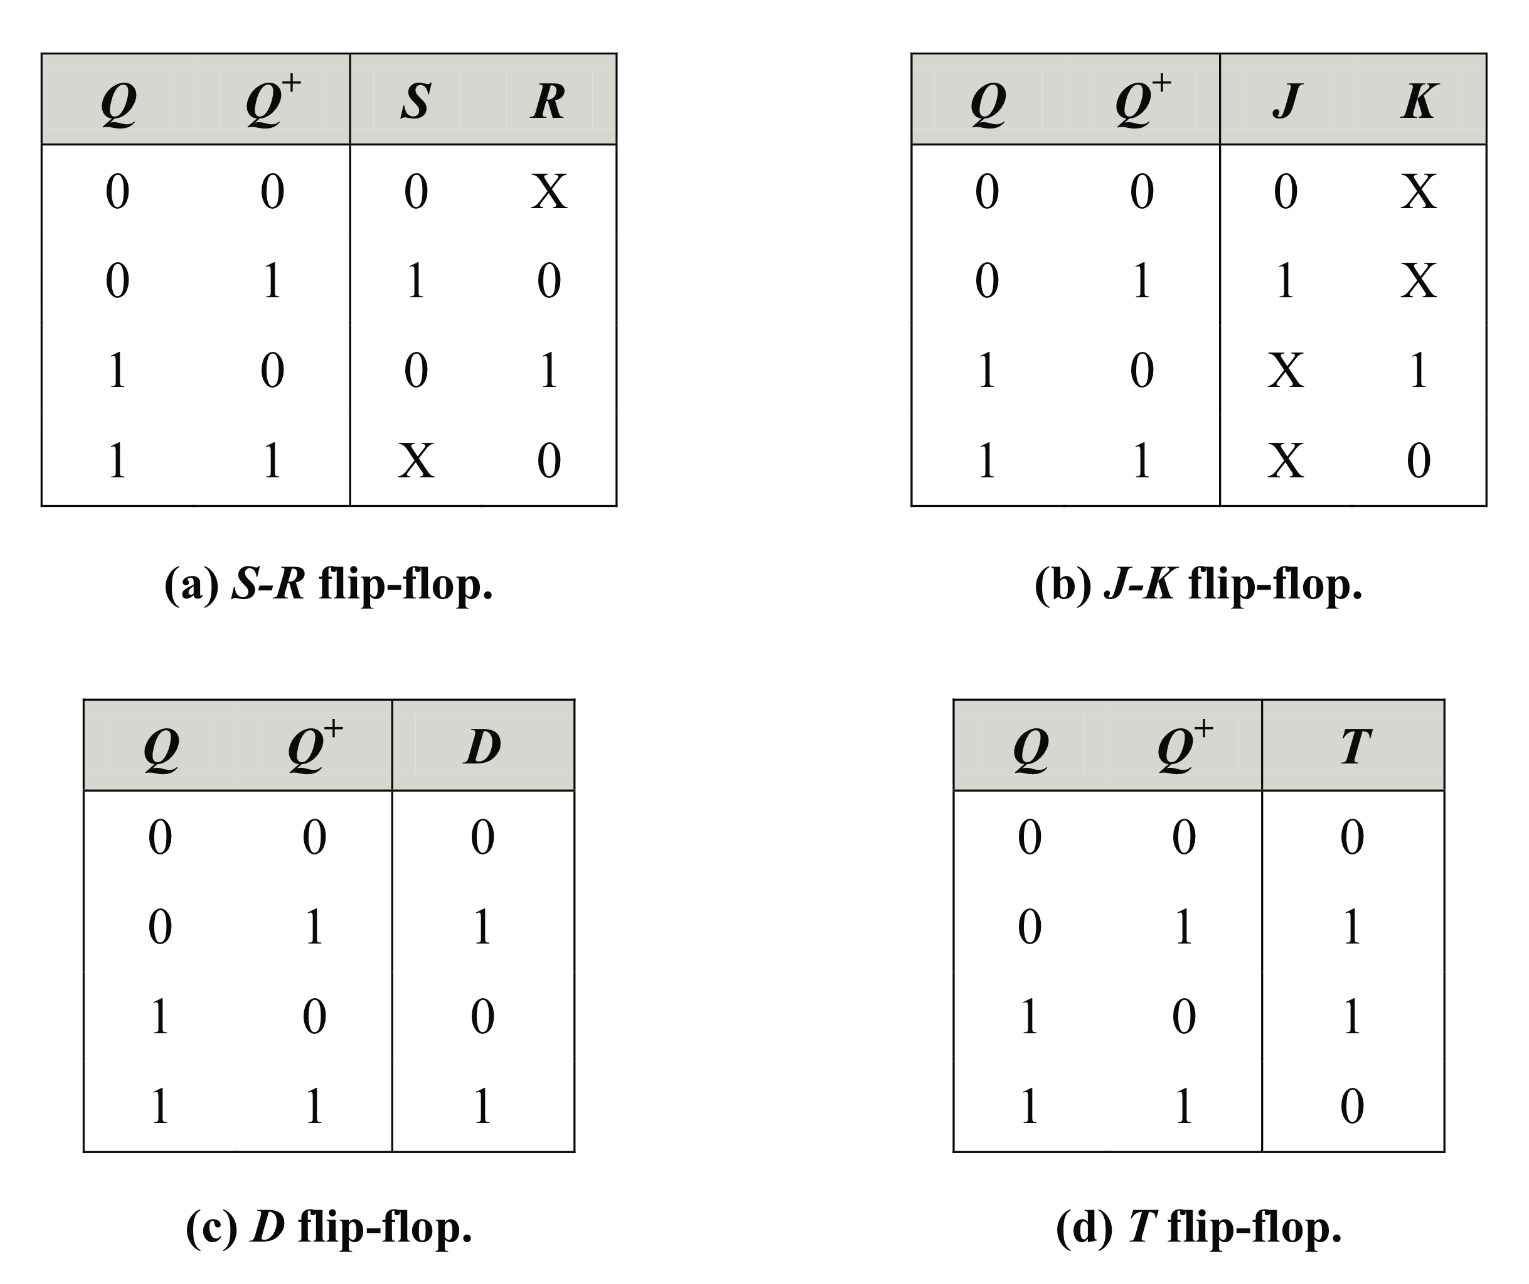
\includegraphics[width=0.5\textwidth]{seq_des}
\end{figure}
\vspace{-4mm}
Given a set of specifications in the form of state equations, state table, or
state diagram, we may derive a logic circuit fulfilling the specifications with
the following procedure:
\begin{enumerate}
  \item Derive the state table of the sequential circuit.
  \item Reduce states if necessary, removing duplicate states having
    identical outputs and next states.
  \item Assign a unique binary value to each state, if the given specifications
    depict states as labels (such as $X$, $Y$, $Z$)
  \item Determine the number of flip-flops required and label them. In general,
    a circuit with $n$ states require $\lceil{\log_2 n}\rceil$ flip-flops
  \item Using the excitation tables and the state tables, choose the
    appropriate type(s) of flip-flops to be used.
  \item Simplify the expressions of the flip-flop input functions and outputs.
  \item Draw the logic diagram of the circuit.
\end{enumerate}
\subsection{Memory}
Given these sequential circuits, we may implement a memory unit of $2^{k}$
words, each word consisting $n$ bits. The memory unit takes in $n$ data input
lines, a $k$-bit address and a $Read/\bar{Write}$ control signal, and provides
a $n$-bit data output.\\
\begin{figure}[h!]
  \centering
  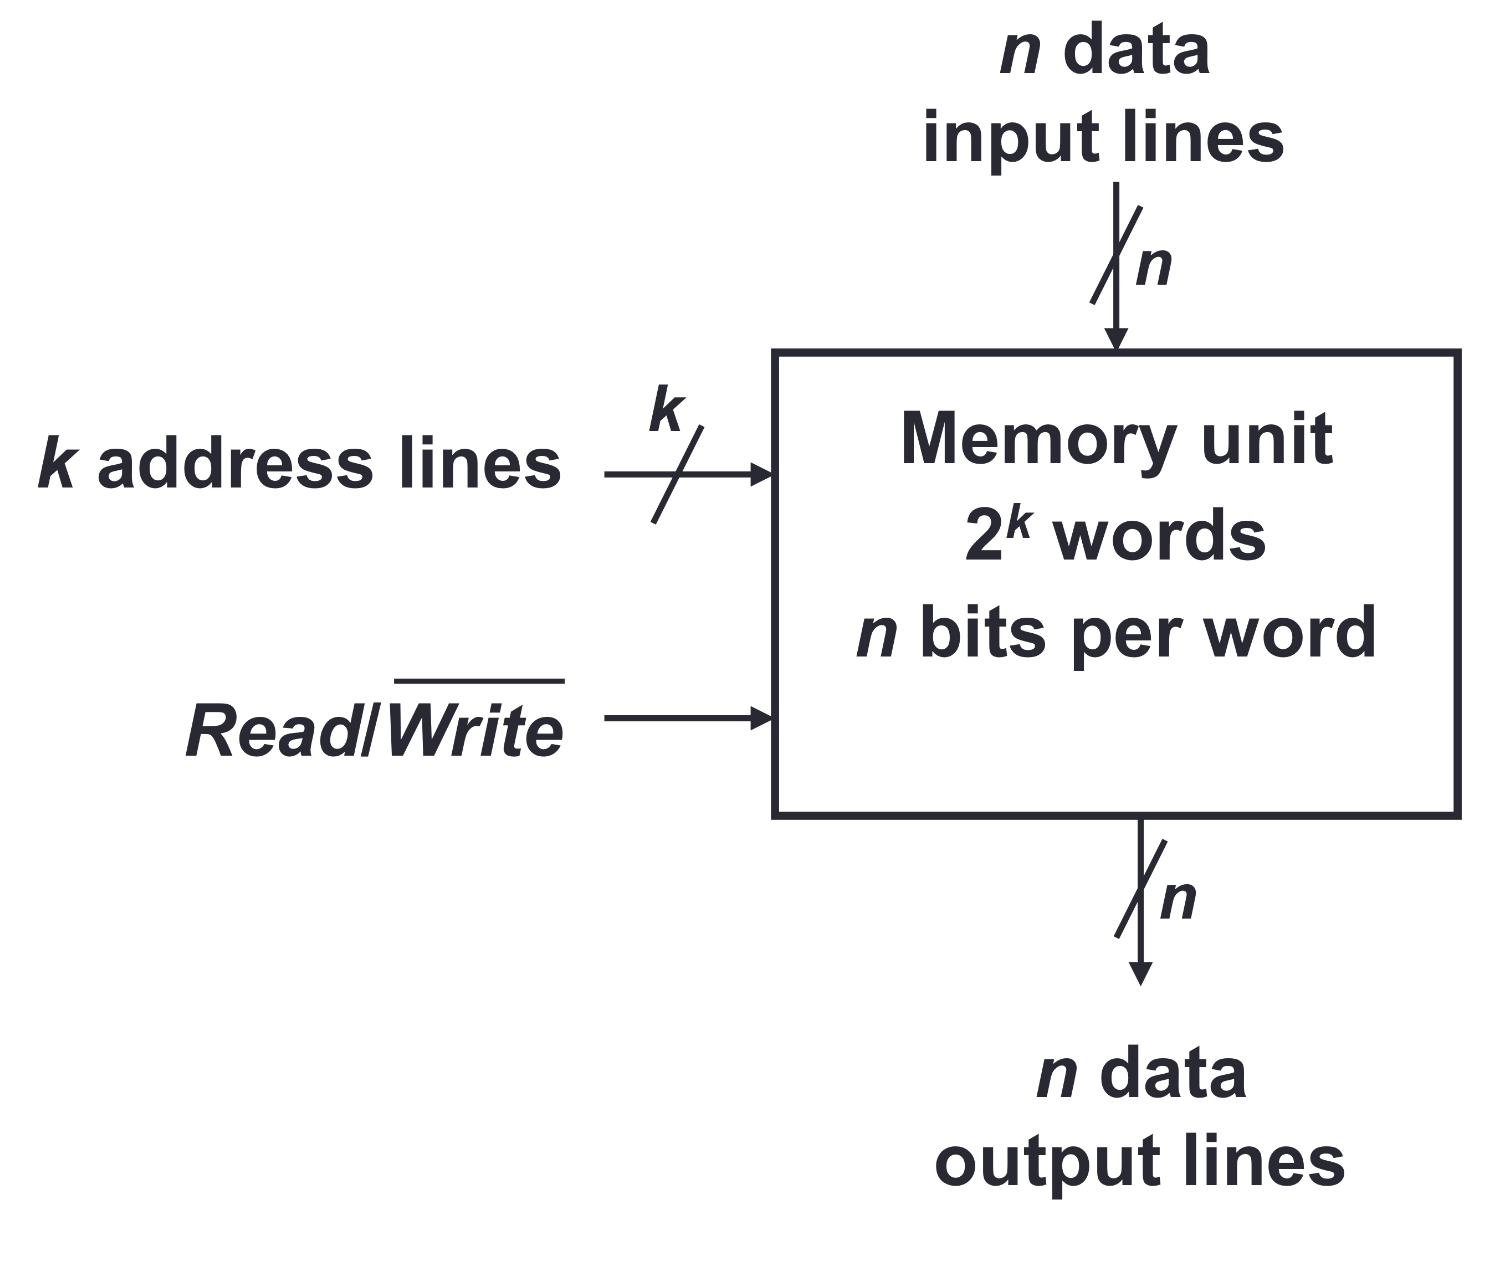
\includegraphics[width=0.3\textwidth]{memory_unit}
\end{figure}
To conduct a Write operation, we have to transfer the address of the desired
word to the address lines, the data bits to be stored to the data input lines,
and the Write control line. Similarly, to conduct a Read operation, we have to
transfer the address of the desired word to the address lines, and activate the
Read control line.

\paragraph{RAM} In general, there are two types of RAM: static RAMs that uses
flip-flops as memory cells, and dynamic RAMs that use capacitor charges to
represent data. DRAMs are simpler in circuitry but have to be constantly
refreshed.
\begin{figure}[h!]
  \centering
  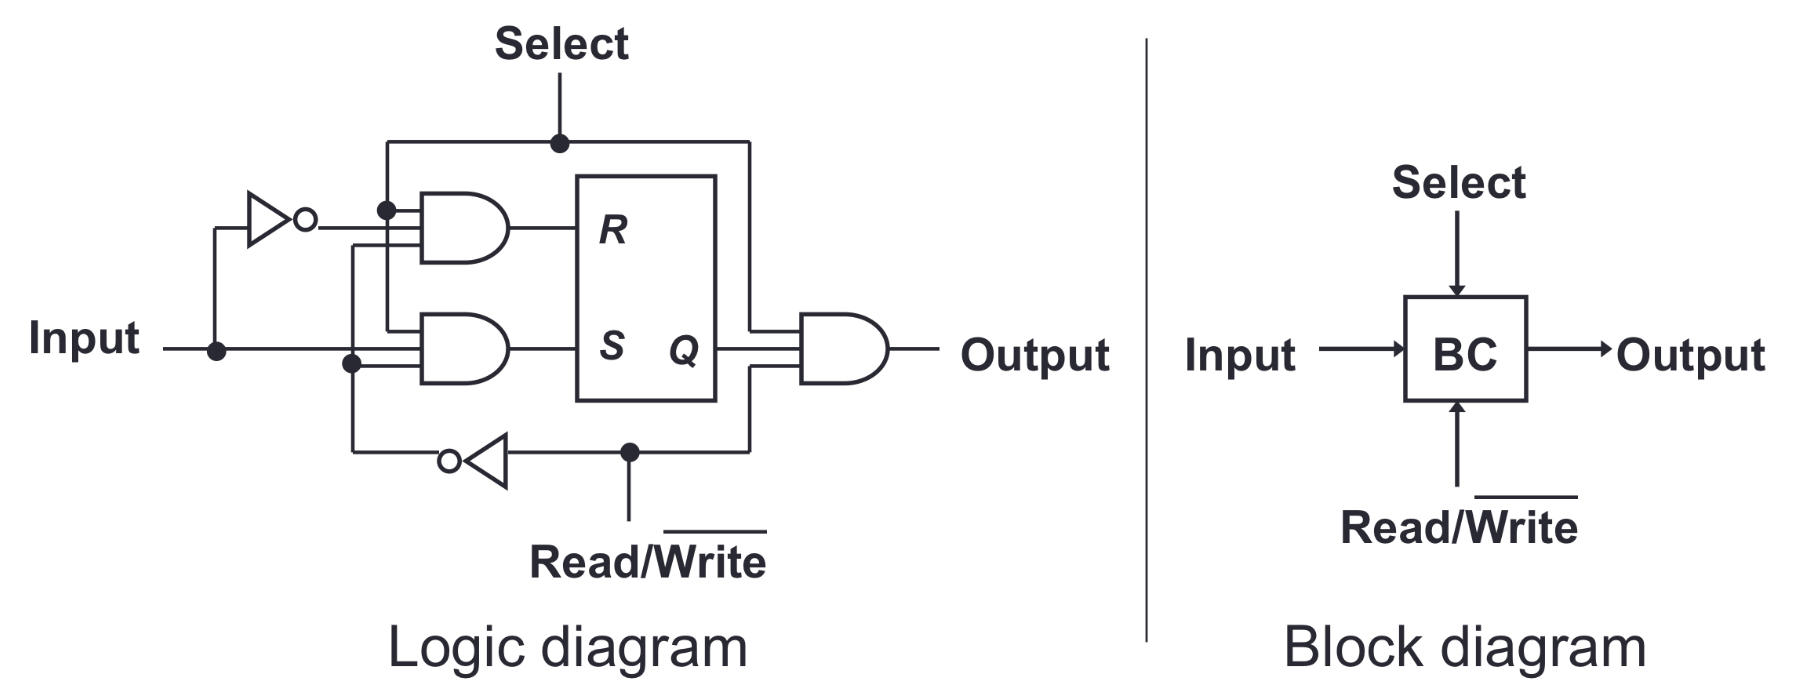
\includegraphics[width=0.49\textwidth]{ram}
  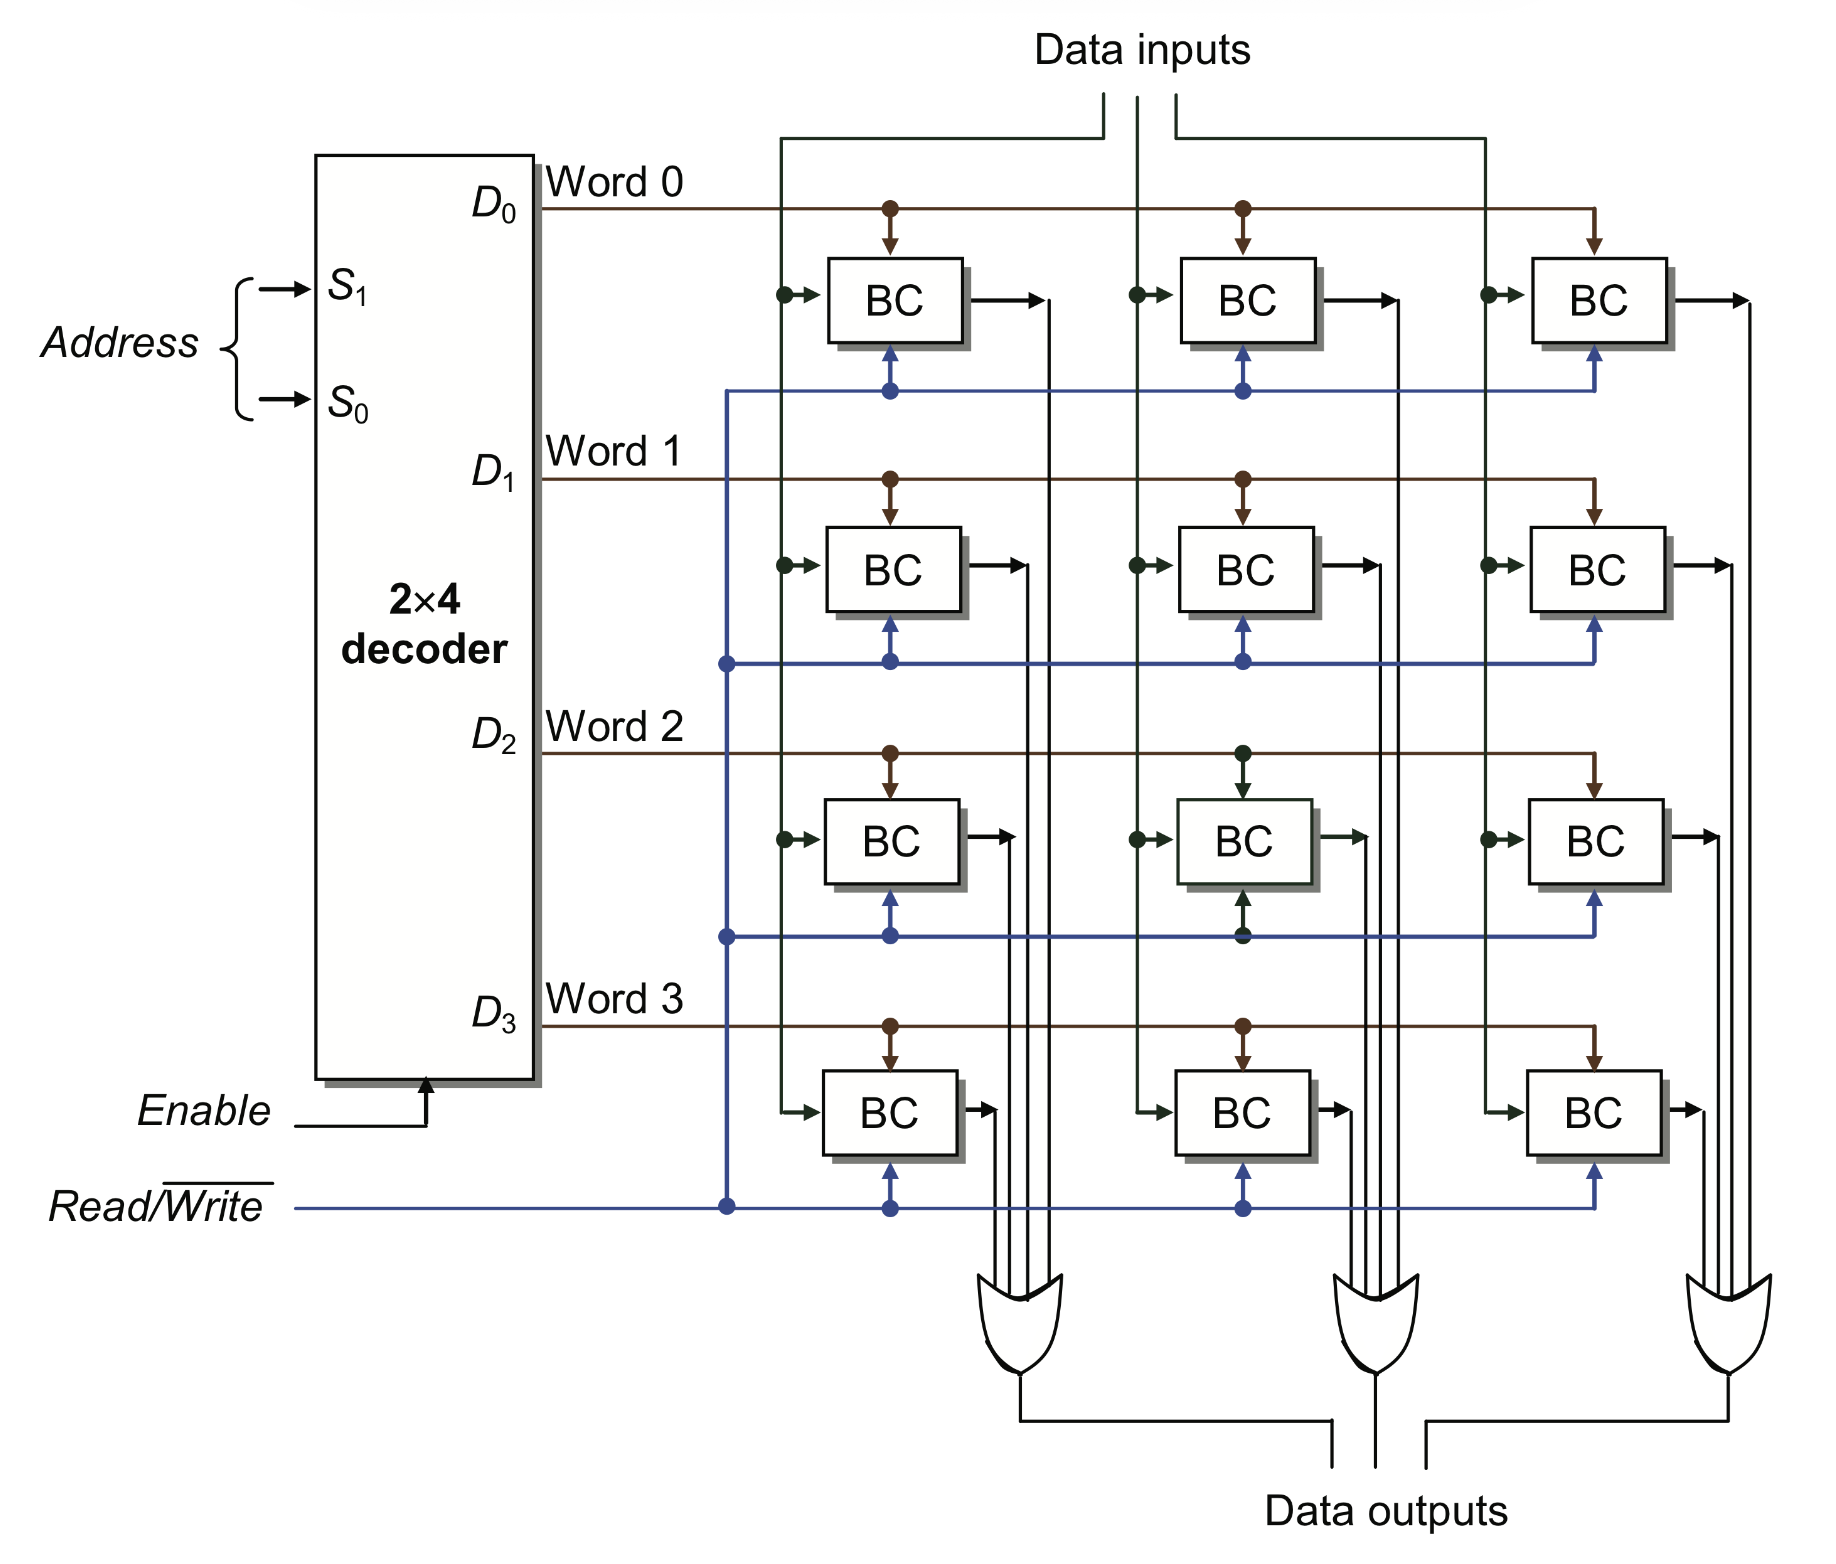
\includegraphics[width=0.5\textwidth]{ram2}
\end{figure}\\
A $4\times 3$ RAM (4 addresses and word size 3) can be constructed with a
circuit with a decoder and OR gates for outputs.
\begin{figure}[h!]
  \centering
  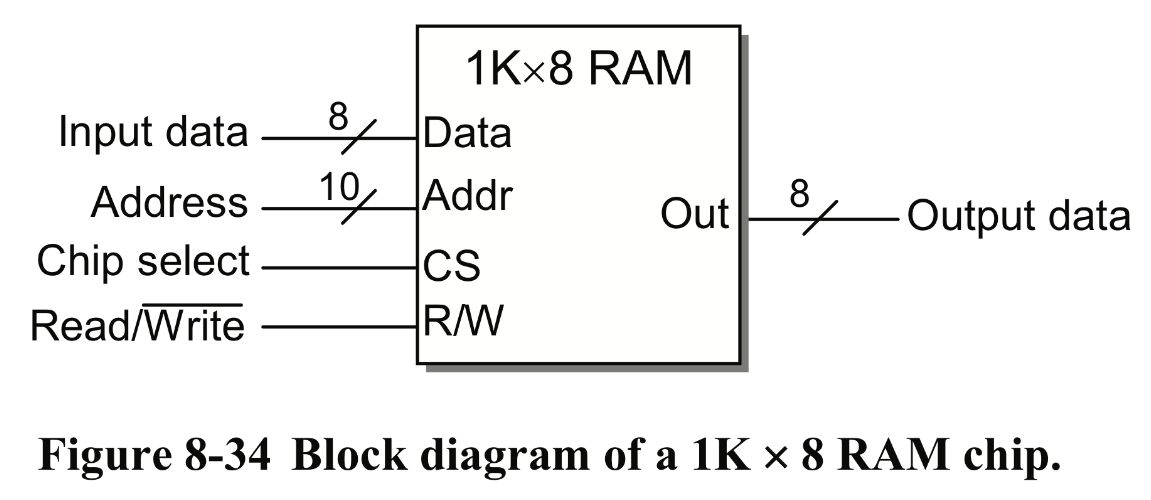
\includegraphics[width=0.4\textwidth]{ram3}
  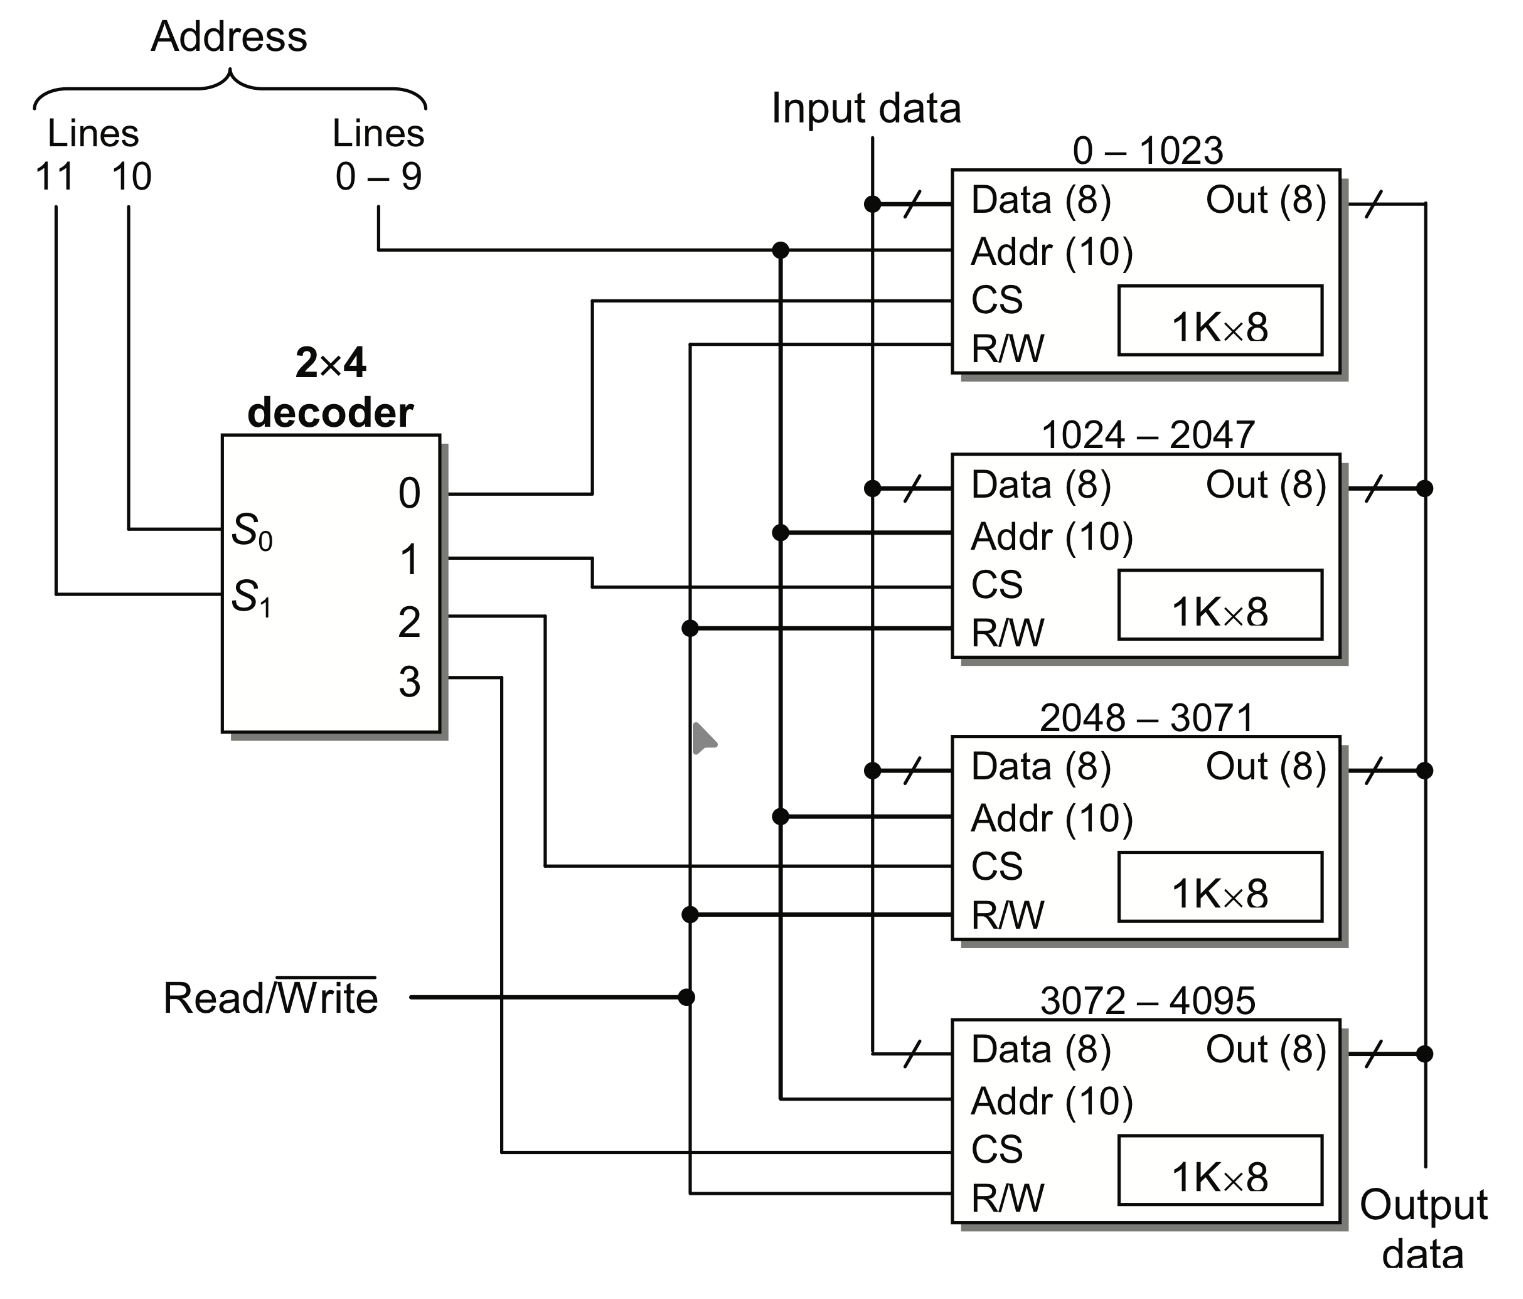
\includegraphics[width=0.5\textwidth]{ram4}
\end{figure}\\
With smaller memory units, we can build bigger memory with an array of RAM
chips, by using decoders to select the correct RAM chip using the Chip select
control signals. This arrangement allows us to use more decoders and RAM chips
to arbitrarily expand our RAM storage.
\begin{figure}[h!]
  \centering
  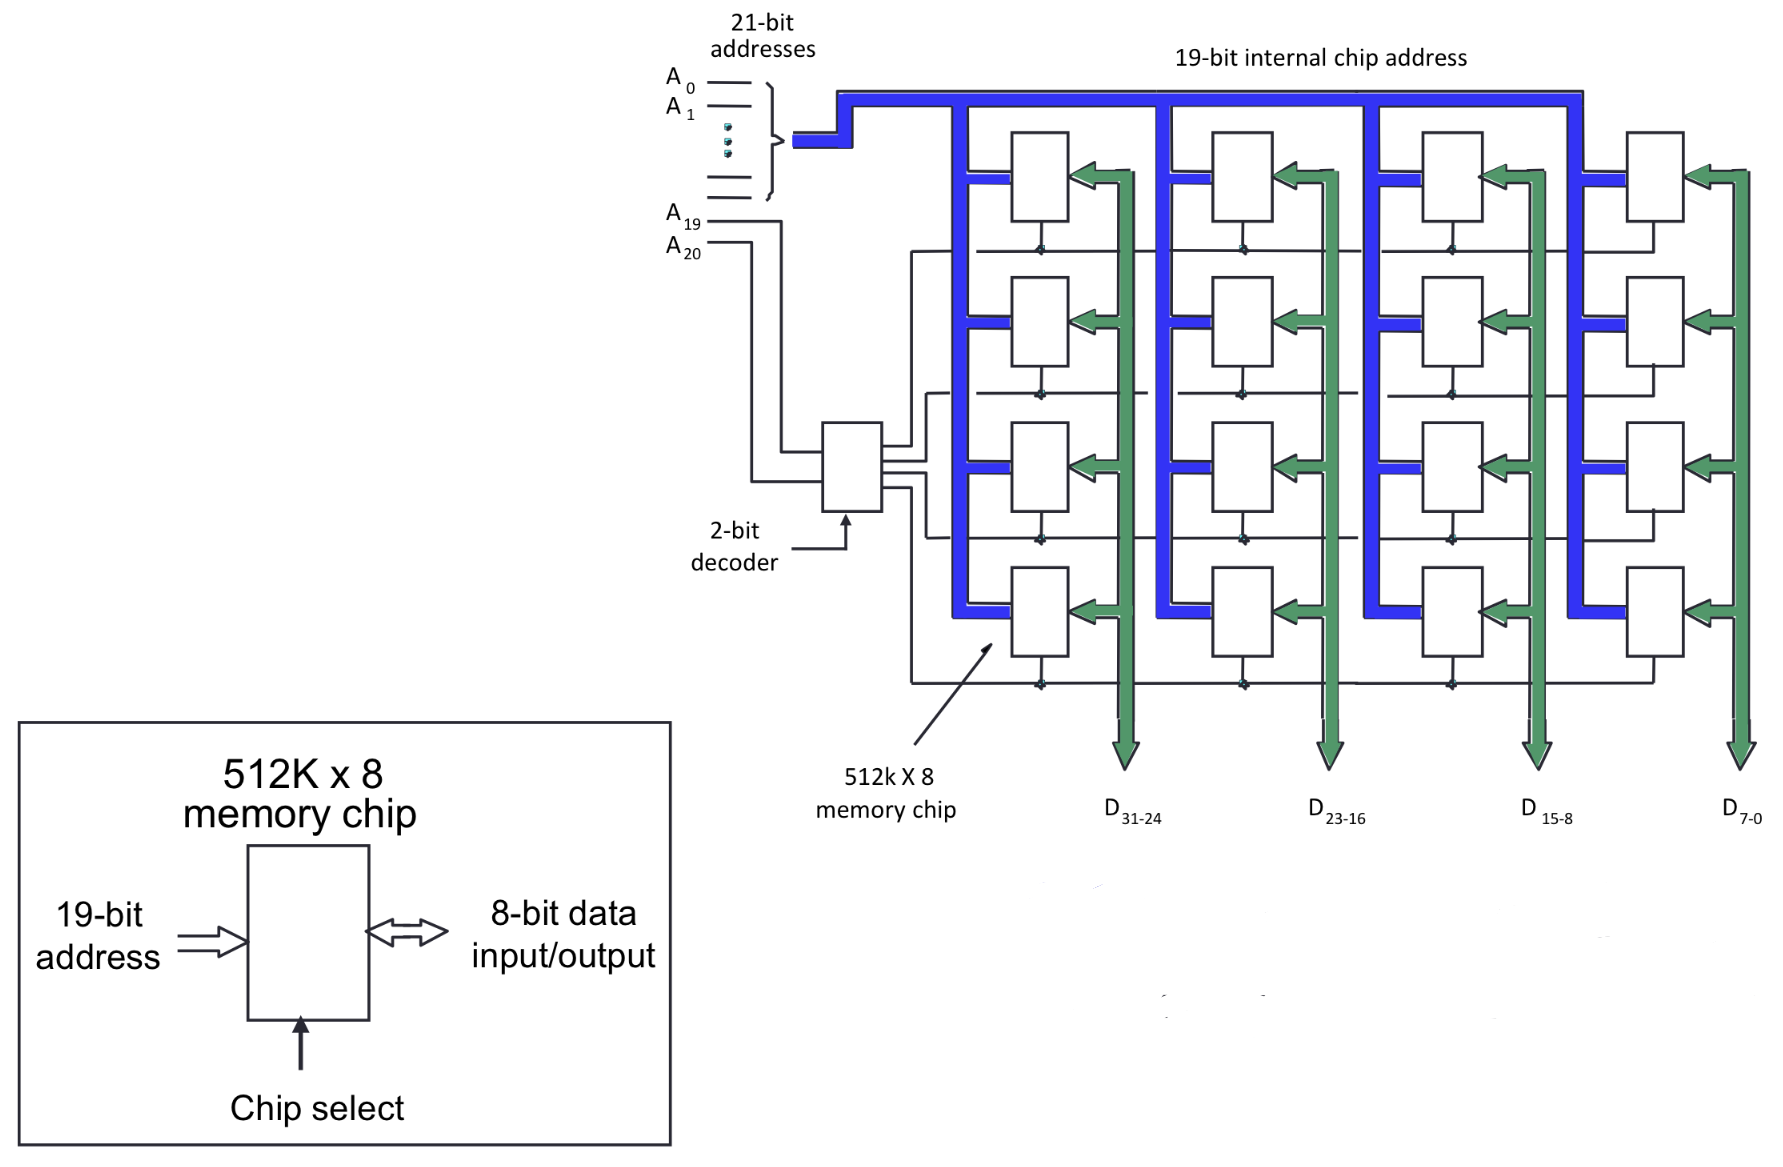
\includegraphics[width=0.7\textwidth]{ram5}
\end{figure}

\section{Pipelining}
Pipelining is an implementation of instruction execution, splitting each
instruction into execution stages, enabling the concurrent execution of
multiple instructions (at different execution stages). Pipelining
\textbf{increases the throughput of the entire workload} without decreasing
latency of any single task, but is \textit{limited by the slowest pipeline
stage} and requires \textit{stalling for dependencies}.\\

In MIPS, each instruction is split into \textbf{five execution stages}:
\begin{itemize}
  \item IF: Instruction Fetch
  \item ID: Instruction Decode and Register Read
  \item EX: Execute an Operation or Address Calculation
  \item MEM: Operand Access in Data Memory
  \item WB: Write Back the Result into a Register
\end{itemize}

\subsection{Implementation: Datapath}
In each cycle, we have the capabilities to execute an instruction in each
pipeline stage. That is, we may execute an instruction currently in the WB
stage, an instruction in the MEM stage, and so on. However, this necessitates
proper transferral and storage of data that is required by the instruction
across the pipeline stages.

\paragraph{Pipeline Registers}
To store the data use by the \textit{same instruction} in later pipeline
stages, the datapath stores additional registers for each of the following
stages: IF/ID, ID/EX, EX/MEM, MEM/WB.
\begin{remark}
  Instructions that do not require certain execution cycles (eg. MEM for ALU
  instructions) still have to go through the pipeline stage.
\end{remark}

\begin{figure}[h!]
  \centering
  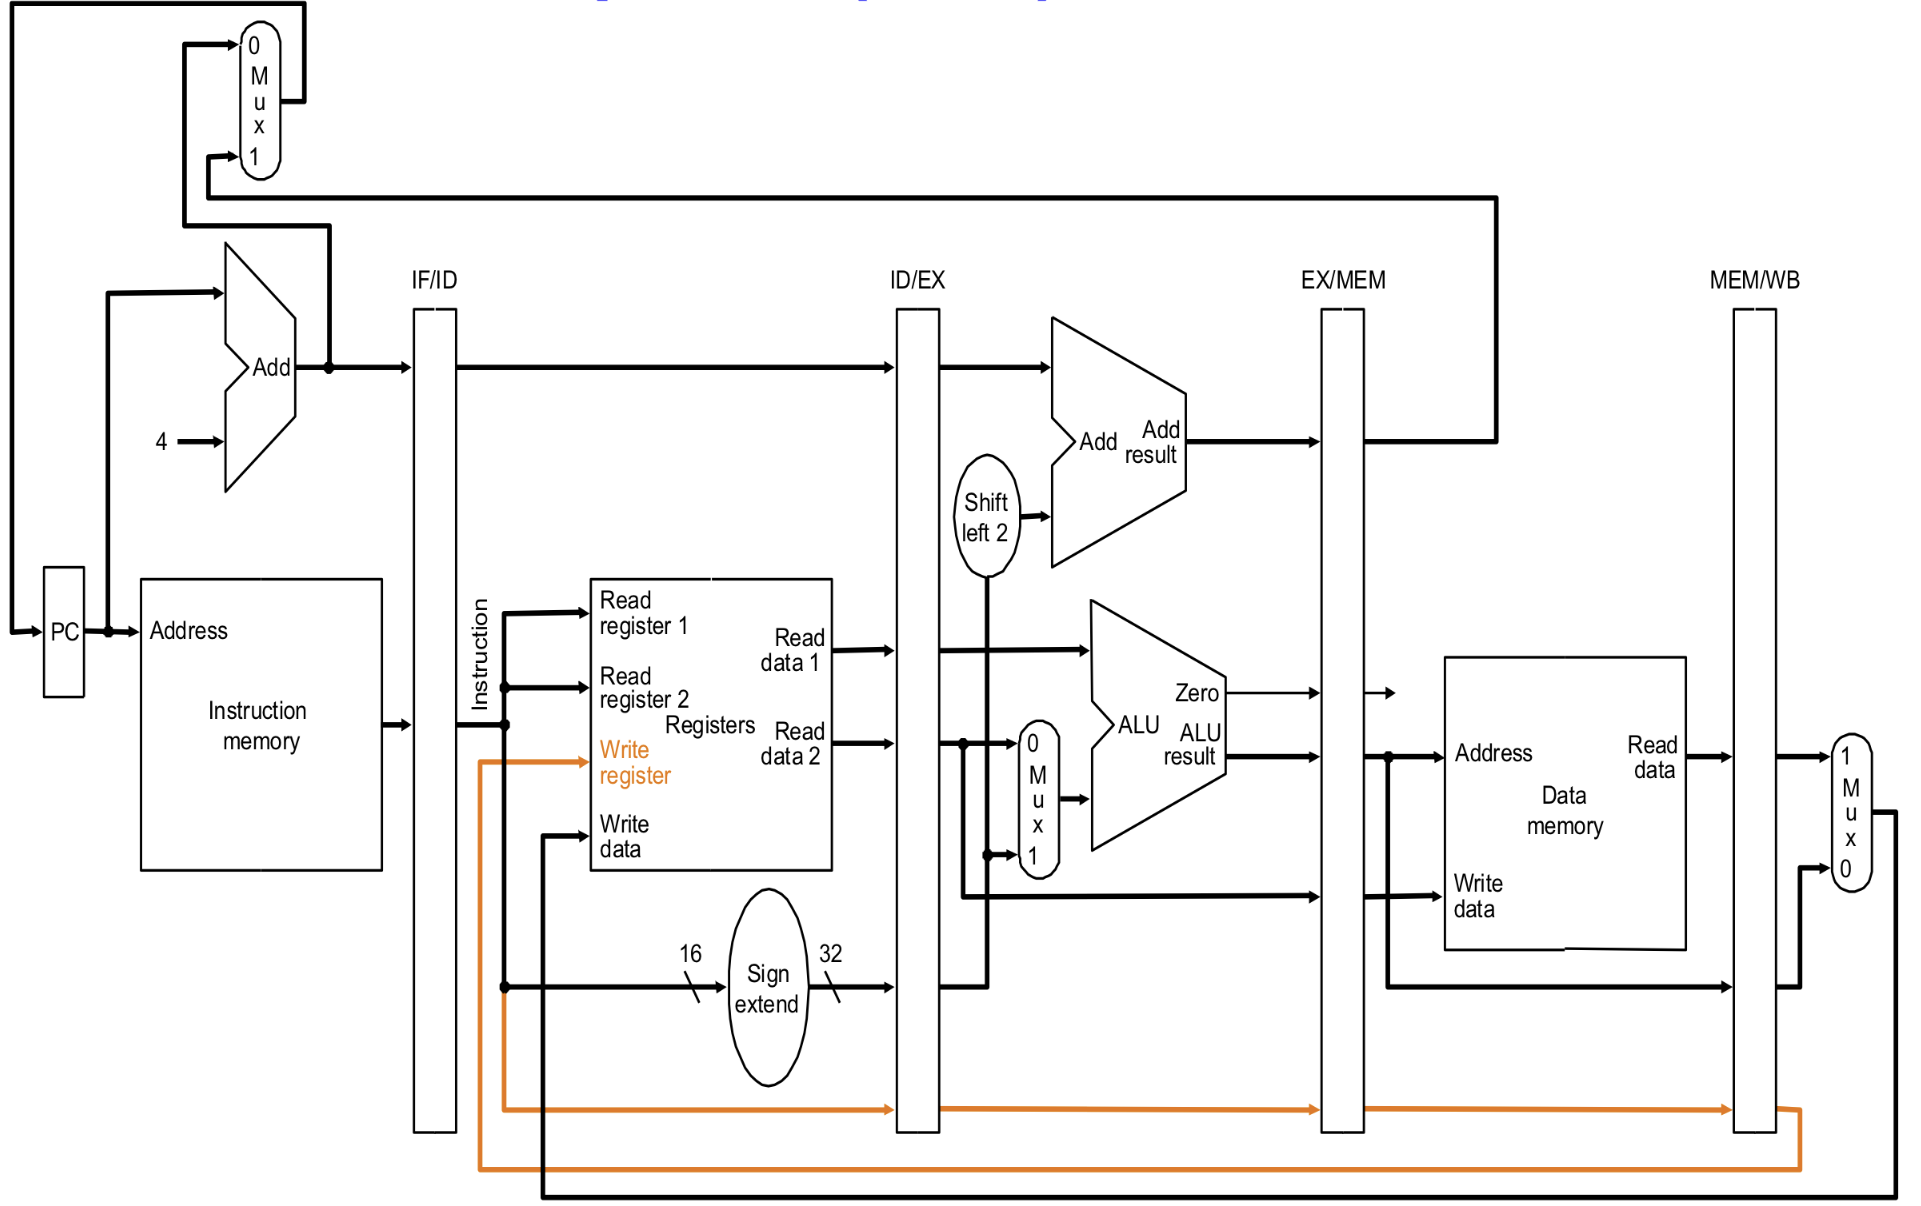
\includegraphics[width=0.8\textwidth]{pipeline_data}
\end{figure}

\paragraph{IF Stage} At the end of a cycle, the IF/ID registers stores:
\begin{itemize}
  \item Instruction read from $InstructionMemory[PC]$
  \item $PC+4$
\end{itemize}

\begin{multicols}{2}
\paragraph{ID Stage} IF/ID registers supplies:
\begin{itemize}
  \item Read Registers for Register File
  \item $16$-bit offset to be sign-extended
  \item $PC+4$
\end{itemize}
ID/EX registers stores:
\begin{itemize}
  \item Read Data from Register File
  \item $32$-bit immediate value
  \item $PC+4$
\end{itemize}
\begin{itemize}
  \item[\vspace{\fill}]
\end{itemize}
\begin{itemize}
  \item Write Register
\end{itemize}
\end{multicols}

\begin{multicols}{2}
\paragraph{EX Stage} ID/EX registers supplies:
\begin{itemize}
  \item Read Data from Register File
  \item $32$-bit immediate value
  \item $PC+4$
  \item Write Register
  \item[\vspace{\fill}]
\end{itemize}
\columnbreak%
EX/MEM registers stores:
\begin{itemize}
  \item $\left( PC+4 \right) + \left( Immediate \times 4 \right) $
  \item ALU Output
  \item \verb|isZero?| Signal
  \item Read Data 2 from Register File
  \item Write Register
\end{itemize}
\end{multicols}

\begin{multicols}{2}
\paragraph{MEM Stage} EX/MEM registers supplies:
\begin{itemize}
  \item $\left( PC+4 \right) + \left( Immediate \times 4 \right) $
  \item ALU Output
  \item \verb|isZero?| Signal
  \item Read Data 2 from Register File
  \item Write Register
\end{itemize}
\columnbreak
MEM/WB registers stores:
\begin{itemize}
  \item ALU Output
  \item Read Data from Data Memory
  \item Write Register
  \item[\vspace{\fill}]
  \item[\vspace{\fill}]
\end{itemize}
\end{multicols}

\paragraph{WB Stage} MEM/WB registers supplies:
\begin{itemize}
  \item ALU Output
  \item Read Data from Data Memory
  \item Write Register
\end{itemize}
At the end of the cycle, result (if any) is written back to register file with
the supplied write register.

\subsection{Implementation: Control}
\begin{figure}[h!]
  \centering
  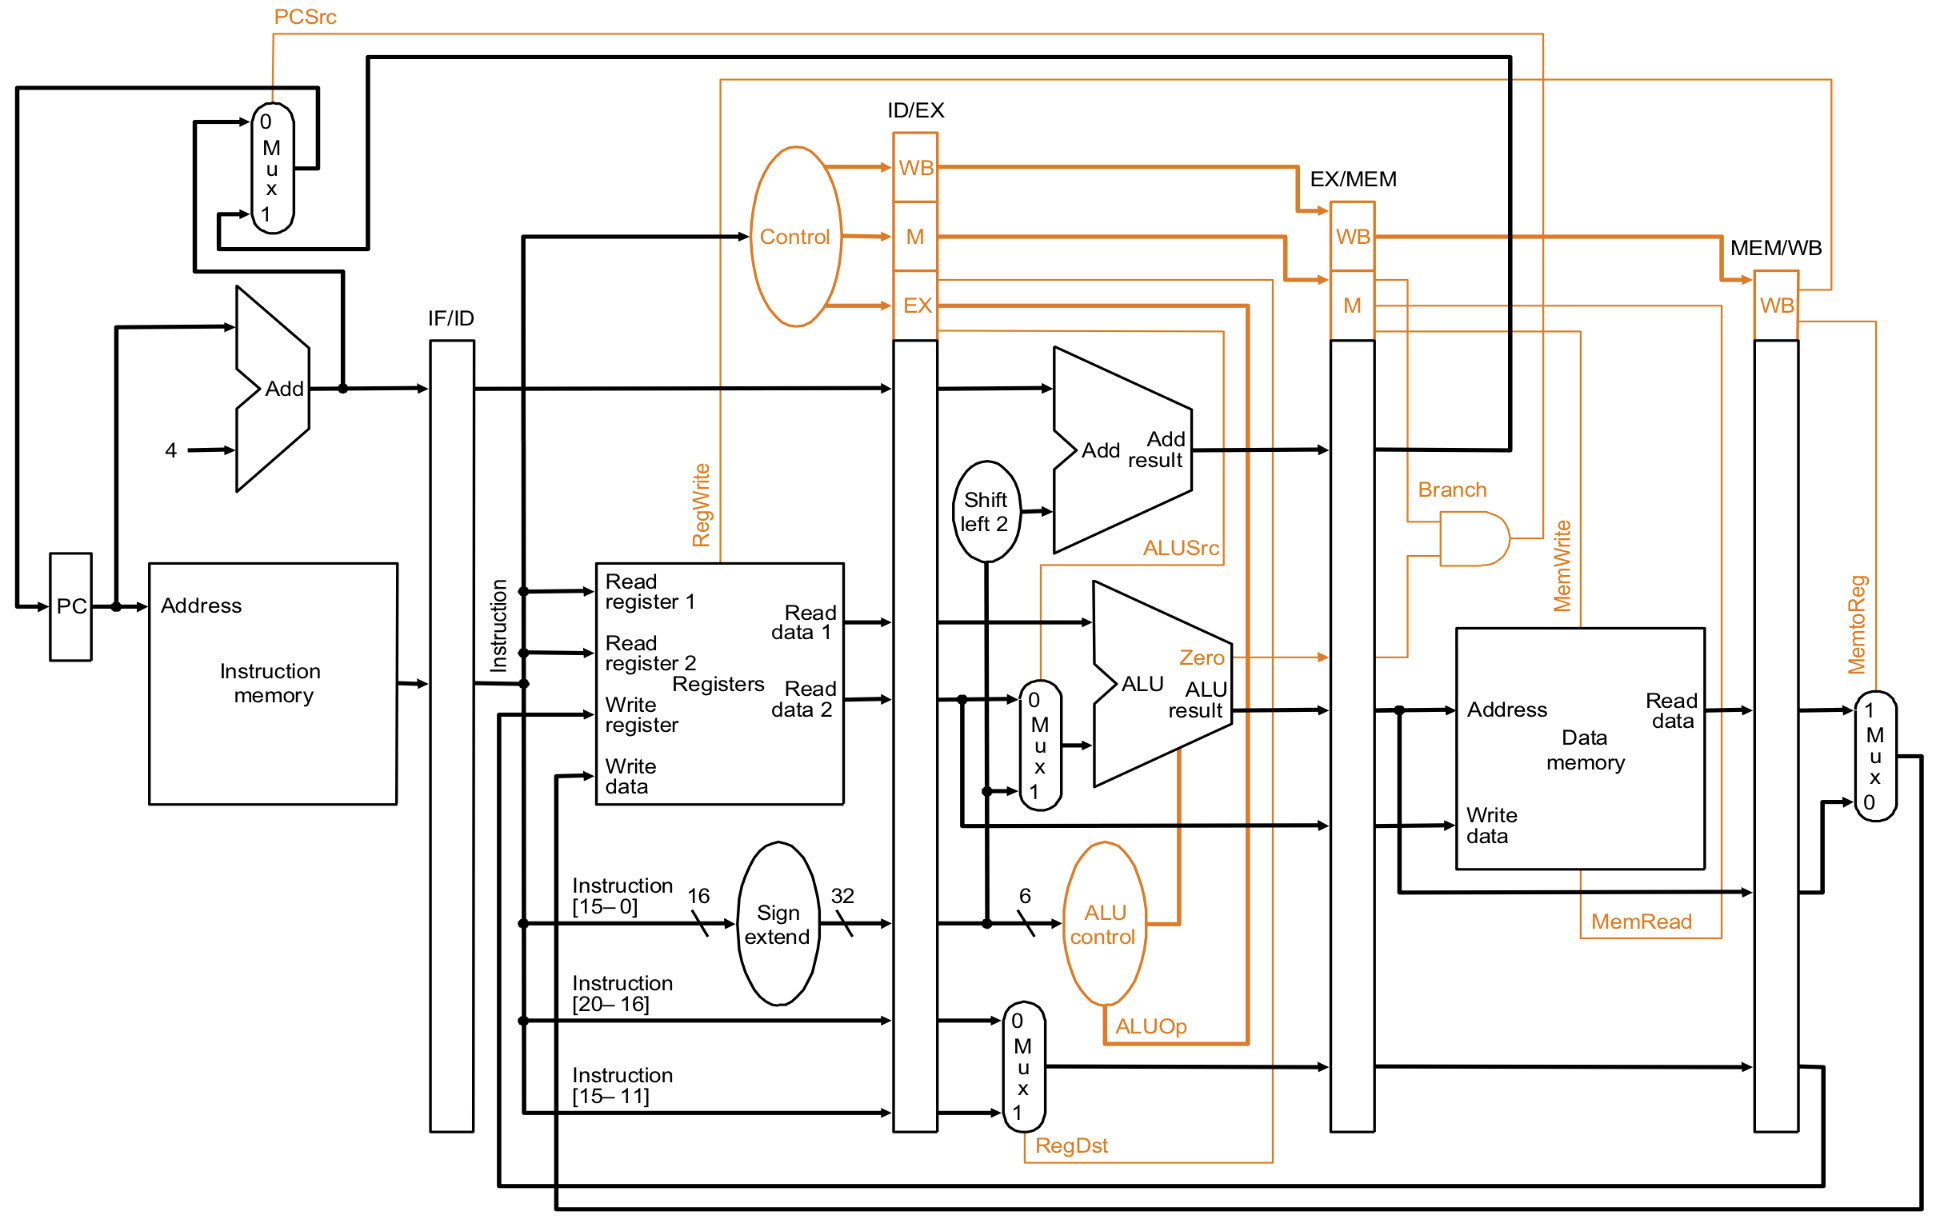
\includegraphics[width=0.8\textwidth]{pipeline_control2}
\end{figure}
The pipeline implementation of control signals is similar to that of a
single-cycle datapath. Each control signal is now associated with a particular
pipeline stage. Since the control signals are generated in the \textbf{ID
stage}, they are propagated through the pipeline registers until utilised.
\begin{figure}[h!]
  \centering
  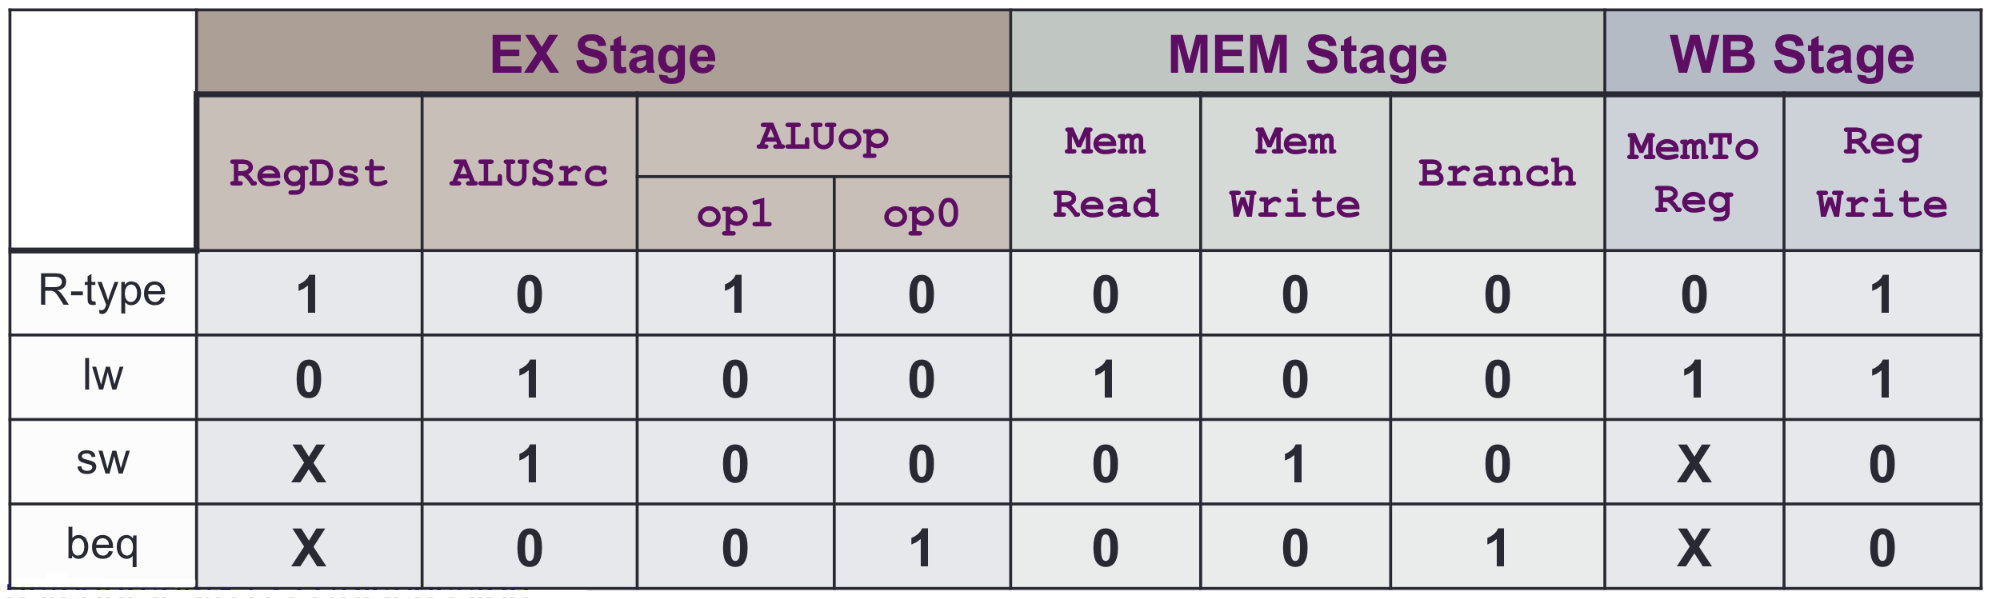
\includegraphics[width=0.7\textwidth]{pipeline_control}
\end{figure}

\subsection{Comparison of Performances}
\begin{figure}[h!]
  \centering
  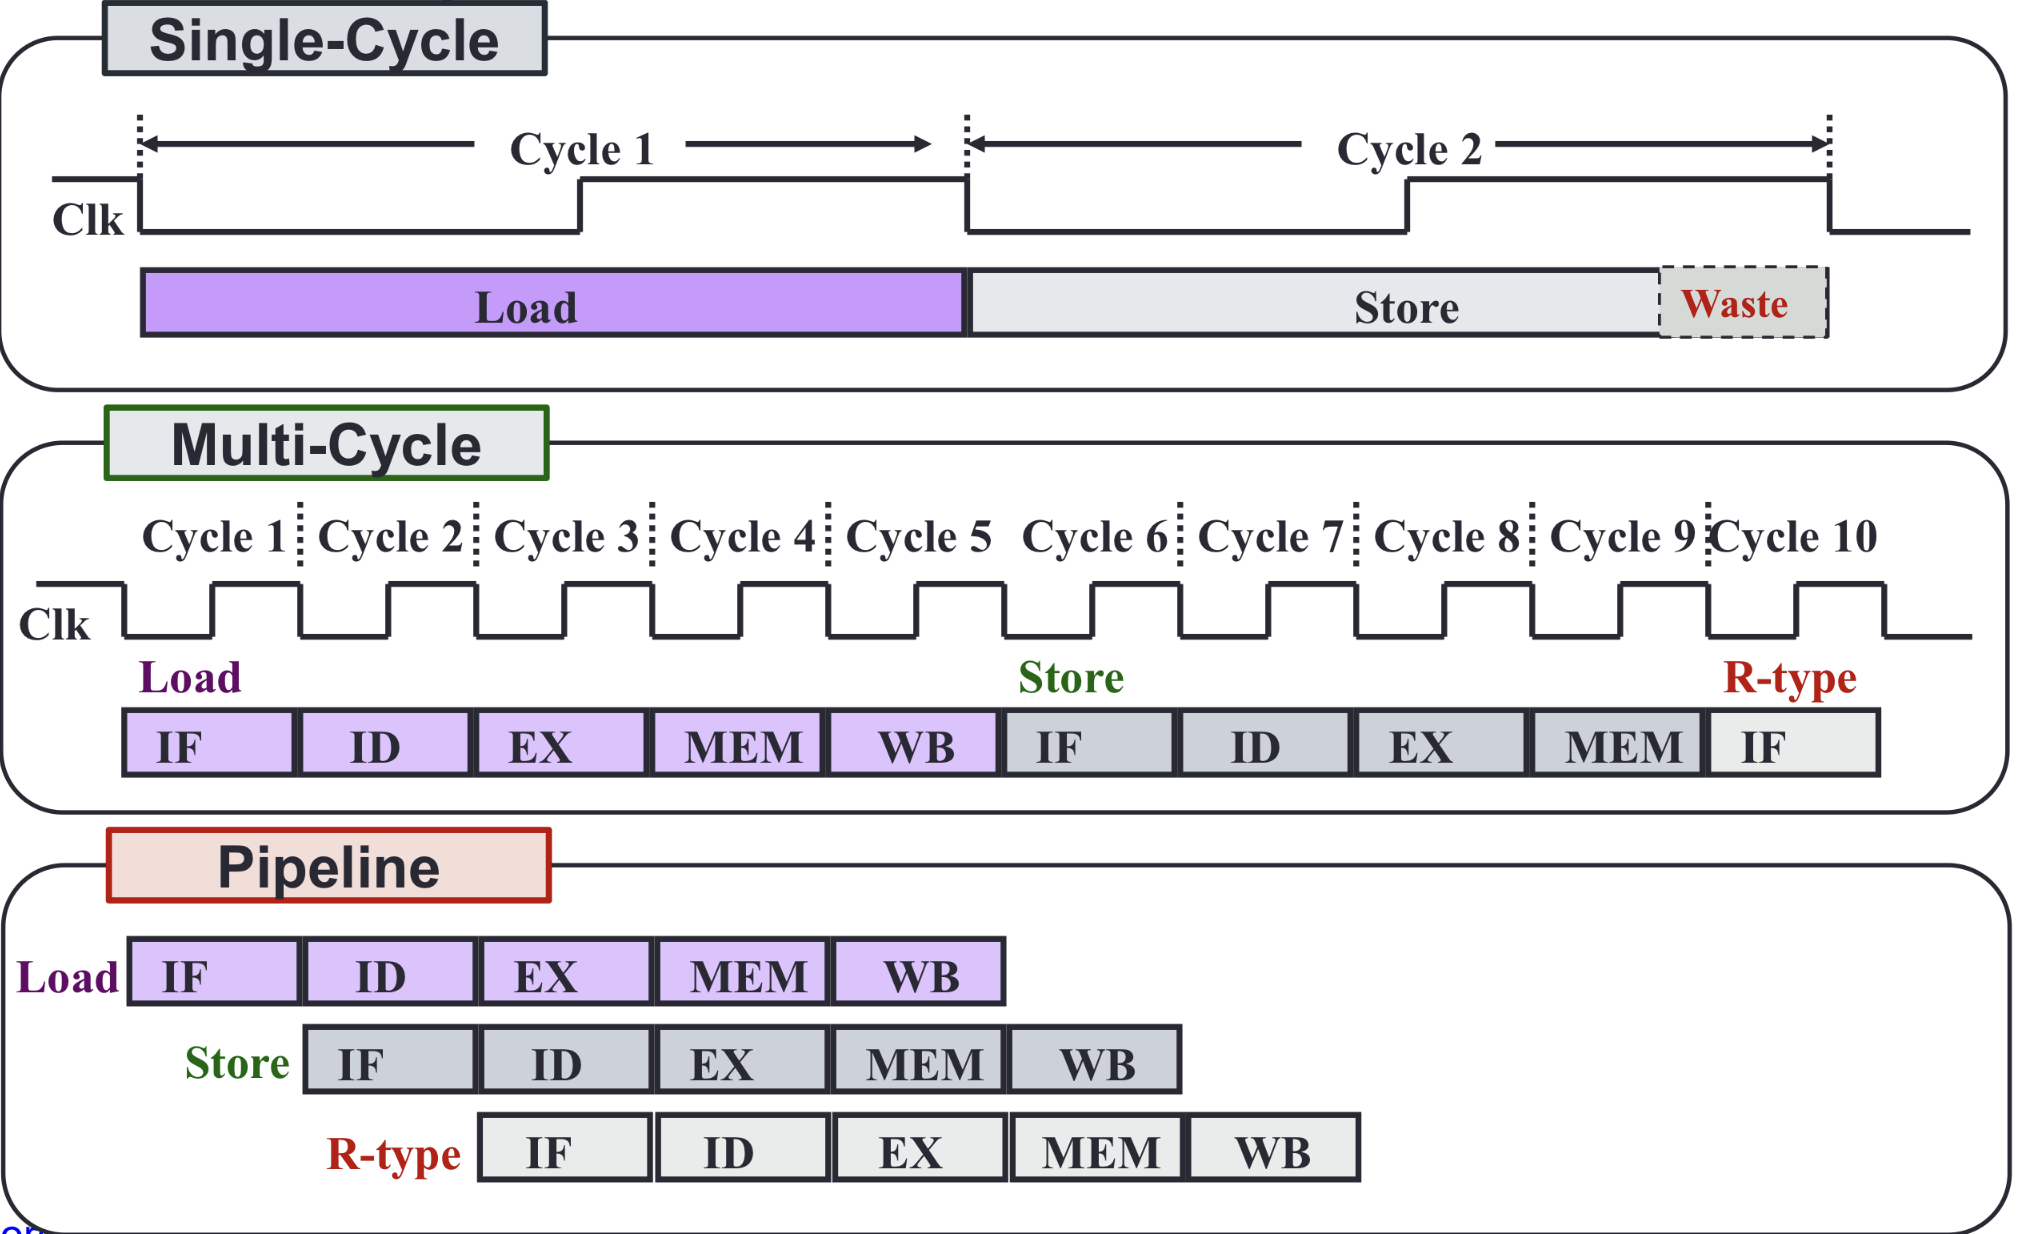
\includegraphics[width=0.5\textwidth]{comparison}
\end{figure}
\paragraph{Single-Cycle Processor}
With a cycle time of
\[CT_{seq}=\max{\left( \sum_{k=1}^{N} T_k \right) }\]
where $T_k$ is the time of operation in stage $k$ and $N$ is the number of
stages, the total execution time for $I$ instructions is
\[Time_{seq}=I\times CT_{seq}.\] 

\paragraph{Multi-Cycle Processor}
With a cycle time of
\[CT_{multi}=\max{\left( T_k \right) }\]
where $T_k$ is the time of operation in stage $k$, the total execution time
for  $I$ instructions is
\[Time_{multi}=I\times Average\ Cycles\ Per\ Instruction\times CT_{multi}.\]

\paragraph{Pipelining Processor}
With a cycle time of
\[CT_{pipeline}=\max{\left( T_k \right) }+T_d\]
where $T_k$ is the time of operation in stage $k$, and $T_d$ is the overhead
for pipelining, the total number of cycles needed for $I$ instructions is
$I+N-1$ (where $N$ is the number of stages), and the total execution time is
\[Time_{pipeline}=\left( I+N-1 \right)\times CT_{pipeline}.\] 
In an ideal case of pipelining, where:
\begin{itemize}
  \item Every stage takes the same amount of time. $\sum_{k=1}^{N} T_k=N\times T_k$
  \item No pipeline overhead. $T_d\to 0$
  \item Number of instructions is much larger than number of stages. $I >> N$
\end{itemize}
The pipeline processor can gain $N$ times speedup compared to a single-cycle
processor.

\subsection{Pipeline Hazards}
Pipeline hazards are issues that prevent the next instruction from immediately
being ``pumped'' into the pipeline following the previous instruction. These
can arise from various problems, such as \textbf{structural hazards}
(simultaneous use of a hardware resource), or instruction dependencies such as
\textbf{data hazards} (data dependencies between instructions) and
\textbf{control hazards} (change in program flow).

\subsubsection{Structural Hazards}
To solve structural hazards, we ensure that processes do not access or use the
same ``part'' of the hardware resource at the same time. This can be done in
several ways, such as:
\begin{enumerate}
  \item \textbf{Stalling} the pipeline for a cycle effectively offsets the next
    instructions by 1.
  \item Dividing the hardware resource (eg. Separating instruction memory and
    data memory)
\end{enumerate}
\begin{example}[Register Access]
  In both the EX and WB stages of the pipeline, instructions access the
  register file to read/write into the registers. To prevent problems in the
  case of accessing the same register, we \textit{split the cycle} into a write
  phase, and a read phase. Instructions are allowed to write into the register
  only during the first half of the cycle, and read from the register only
  during the second half of the cycle. This can be be done because registers
  comprises fast memory devices.
\end{example}

\subsubsection{Data Hazards}
Instructions can have various relationships that prevent pipeline execution.
When different instructions access the same register, we have \textbf{data
dependencies} between the instructions.
\begin{definition}[Read-After-Write]
  RAW occurs when a later instruction reads from the destination register which
  is written by an earlier instruction.
\end{definition}
\begin{figure}[h!]
  \centering
  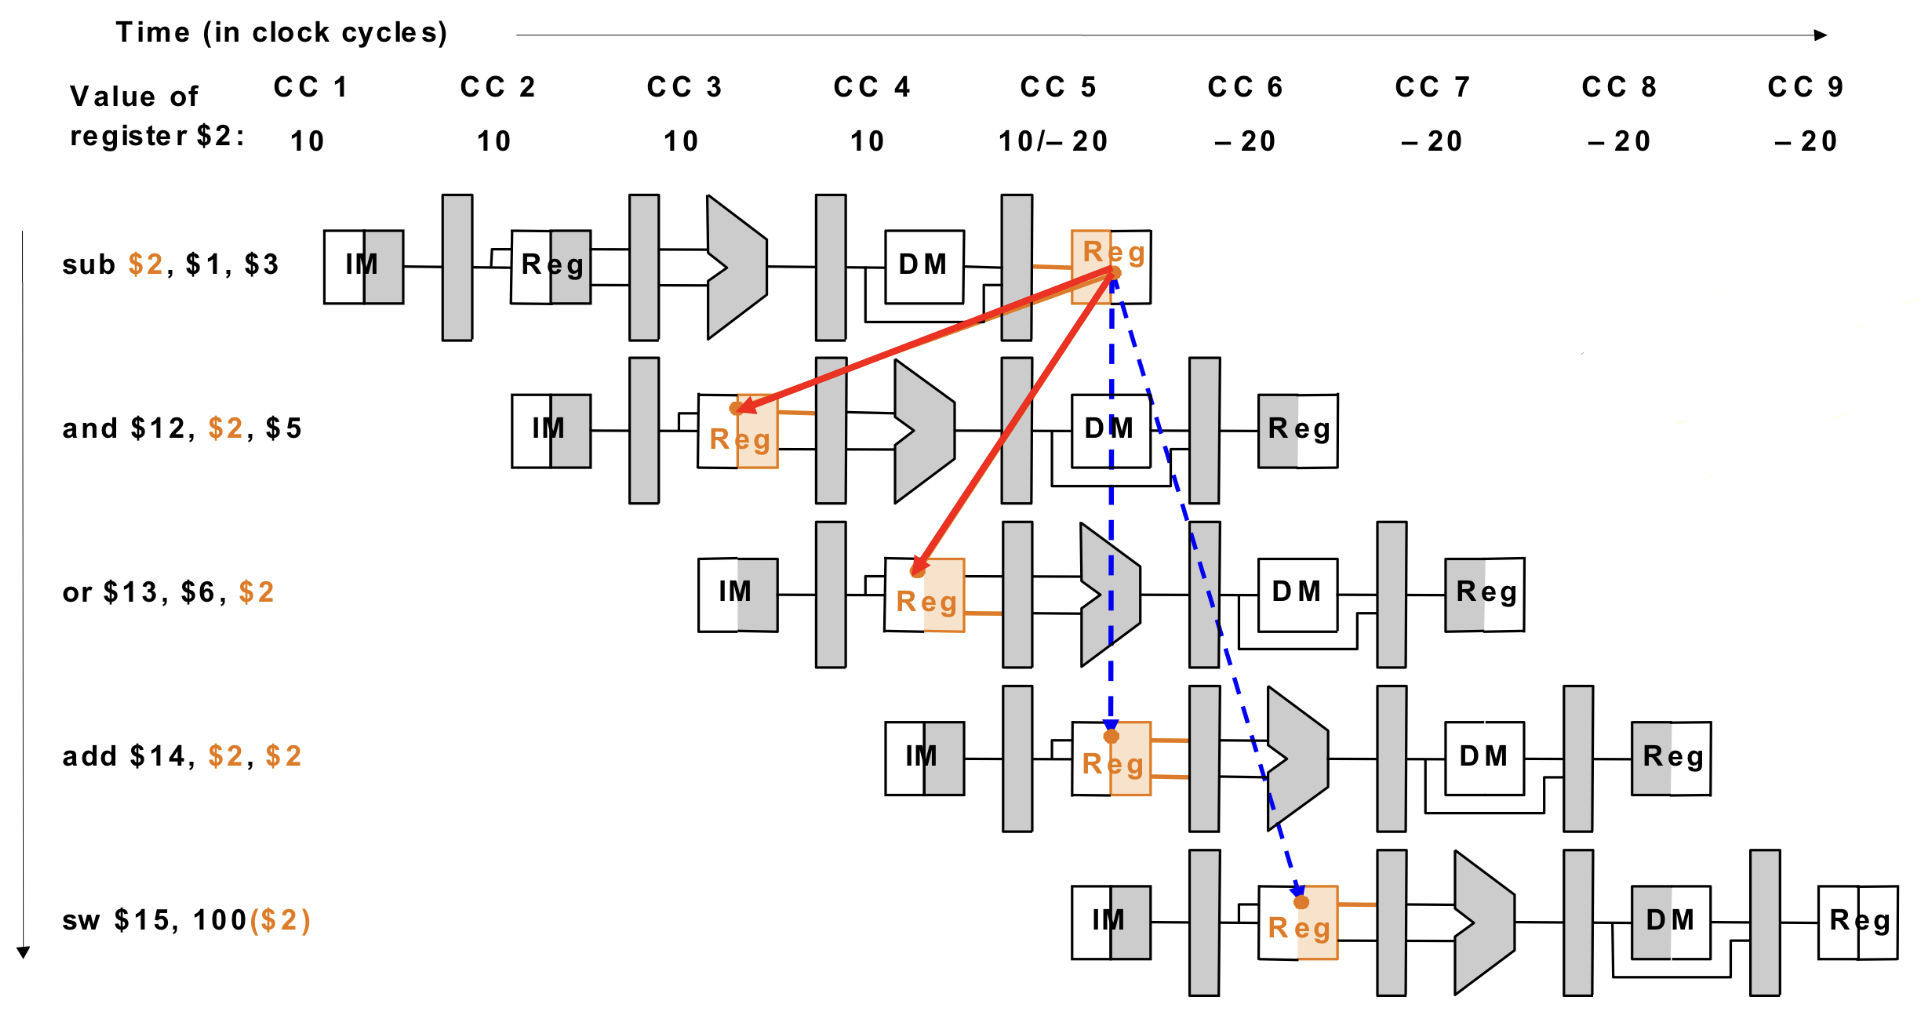
\includegraphics[width=0.6\textwidth]{data_hazard}
\end{figure}
\begin{example}[RAW Data Hazard]
  In the code fragment, the multiple reads of $\$2$ after its initial write
  causes data hazards in the pipeline.
  \begin{lstlisting}
    sub $2, $1, $3
    and $12, $2, $5
    or $13, $6, $2
    add $14, $2, $2
    sw $15, 100($2)
  \end{lstlisting}
\end{example}
\paragraph{Forwarding} If the result is produced before it is used, that is,
the result exists in the pipeline registers, we may forward the result to any
trailing instructions from the pipeline registers, bypassing the read
registers.
\begin{figure}[h!]
  \centering
  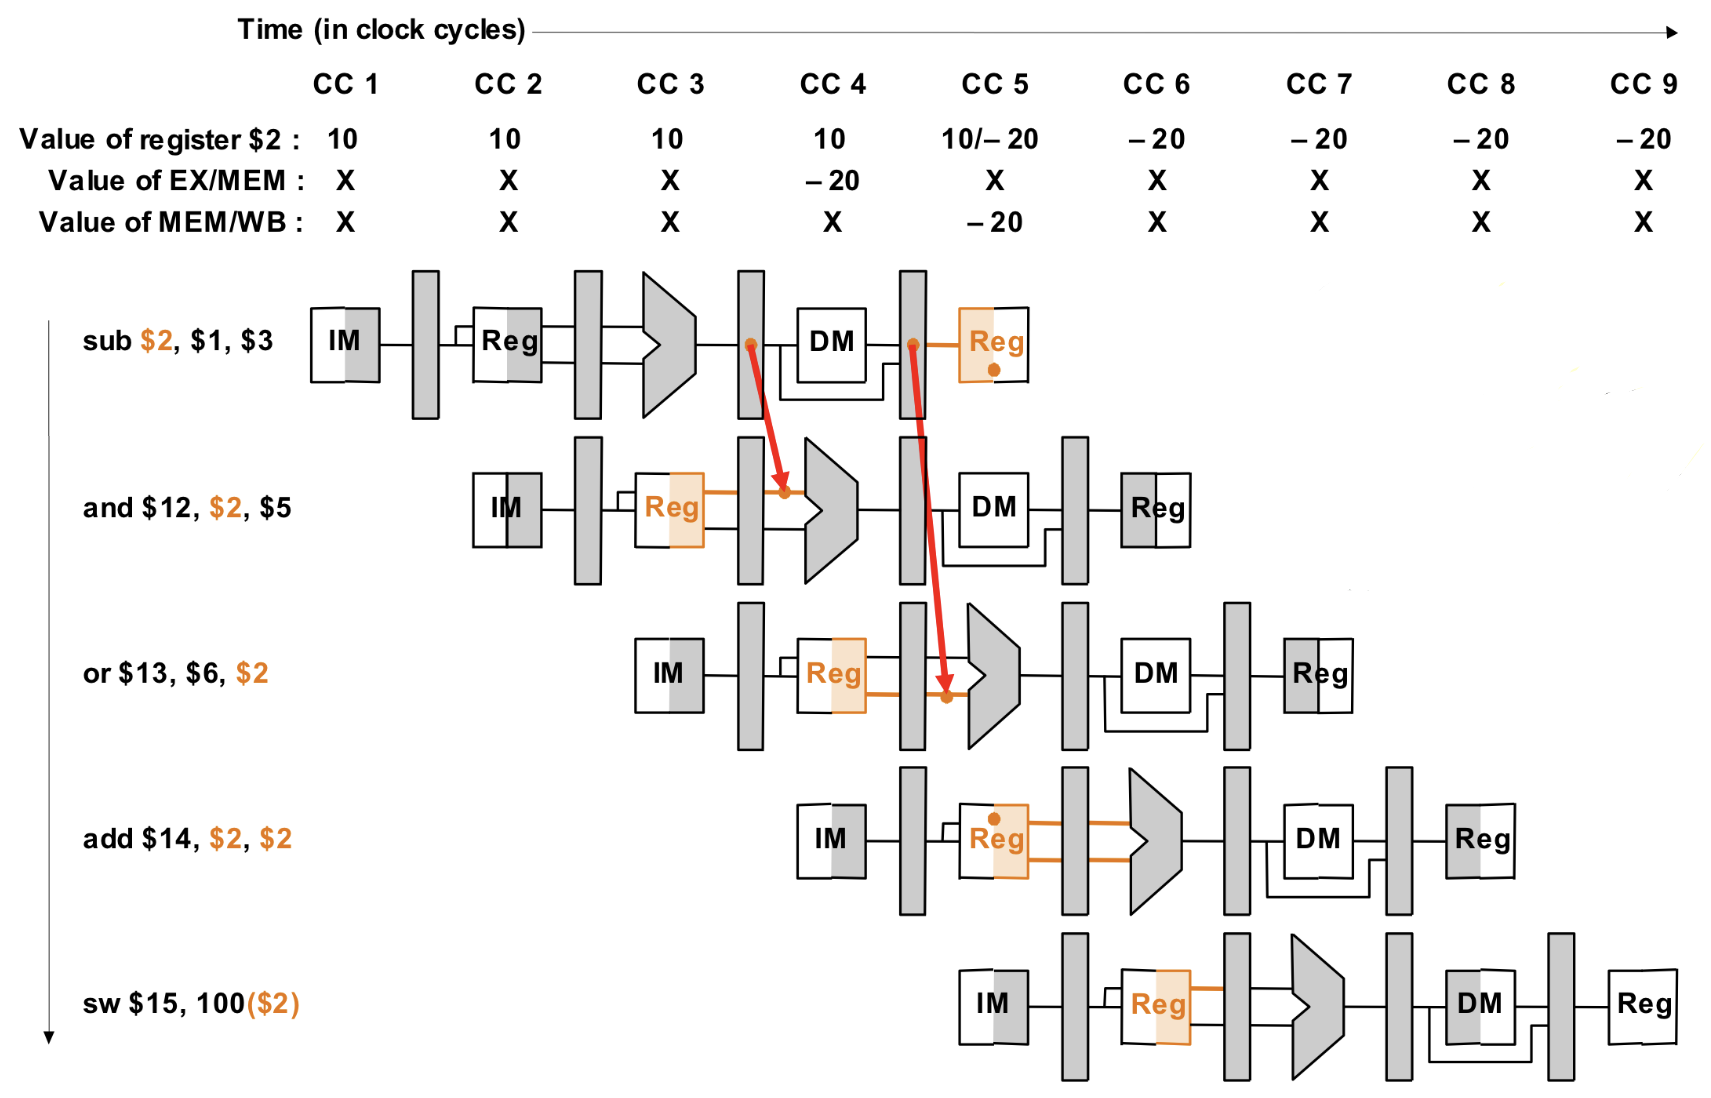
\includegraphics[width=0.6\textwidth]{forwarding}
\end{figure}

\paragraph{Stalling} If the result is produced only in the MEM stage (in a LOAD
instruction), the result is required before it is produced, and we have to stall
the pipeline 
\begin{figure}[h!]
  \centering
  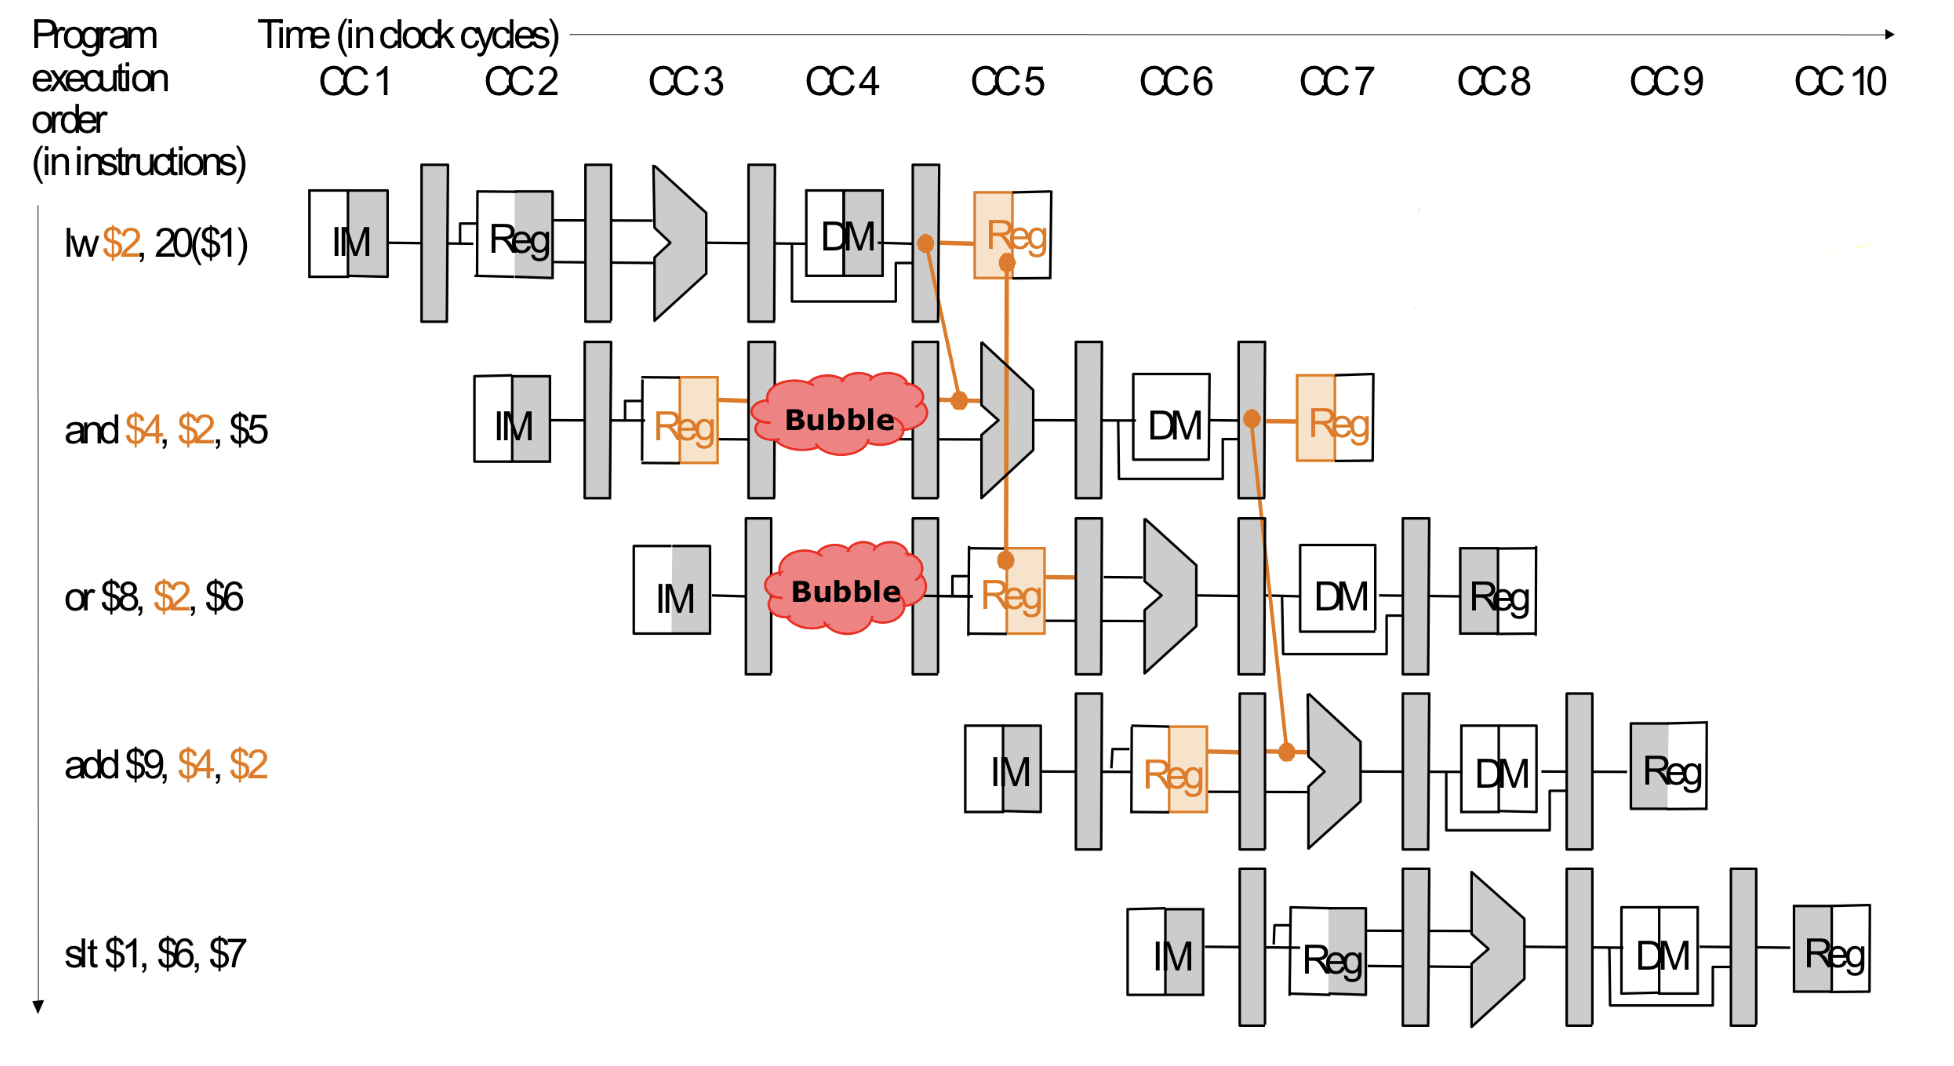
\includegraphics[width=0.5\textwidth]{stalling}
\end{figure}

\begin{remark}
  RAW is also known as true data dependency, as cases of Write-After-Write,
  Write-After-Read, Read-After-Read do not impose a data hazard.
\end{remark}

\subsubsection{Control Hazards}
\begin{definition}[Control Dependency]
  An instruction $j$ is control dependent on $i$ if $i$ controls whether $j$
  executes.
\end{definition}
In particular, the branch and jump instructions introduce control dependencies,
where the branch decision is made only in the MEM stage. The pipeline wrongly
executes 3 instructions and has to be flushed. The 3-cycle penalty can be
mitigated with \textbf{early branch resolution}, \textbf{branch prediction},
and \textbf{delayed branching}.

\paragraph{Early Branch Resolution}
By moving the branch target address calculation and register comparison, we can
make the decision in the ID stage instead of MEM (by creating a semi-ALU to
compare register values). This effectively reduces the delay from 3 to 1 clock
cycle.
\begin{figure}[h!]
  \centering
  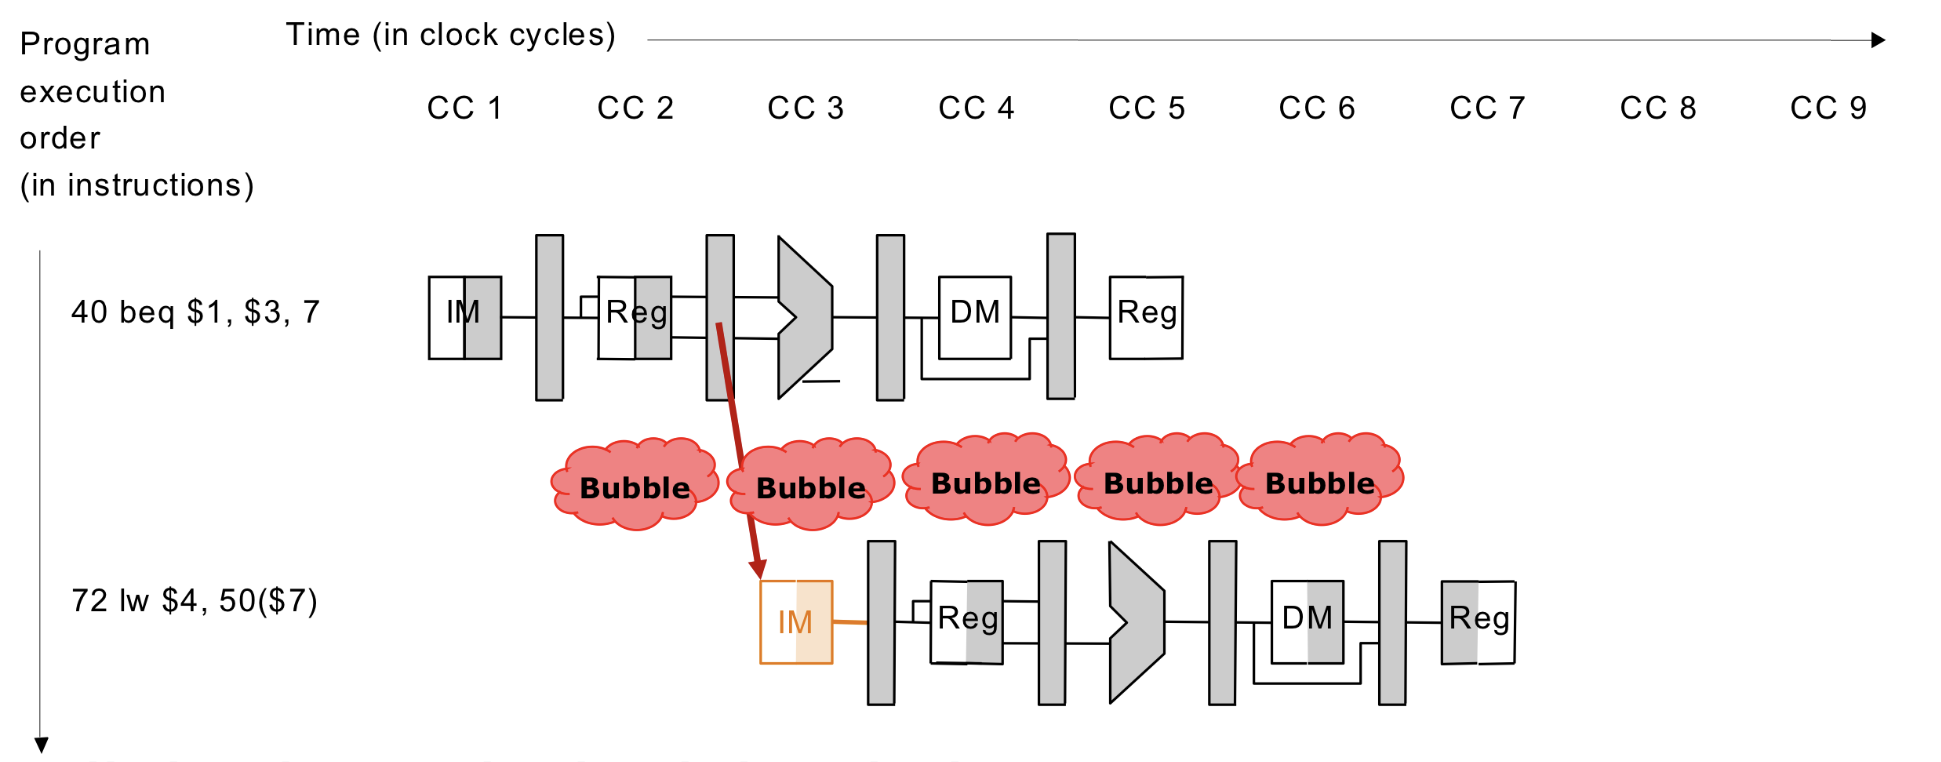
\includegraphics[width=0.8\textwidth]{earlyBranch}
\end{figure}

However, if the registers involved in the comparison is data dependent on
preceding instructions, forwarding is required, introducing further stalls.

\begin{figure}[h!]
  \centering
  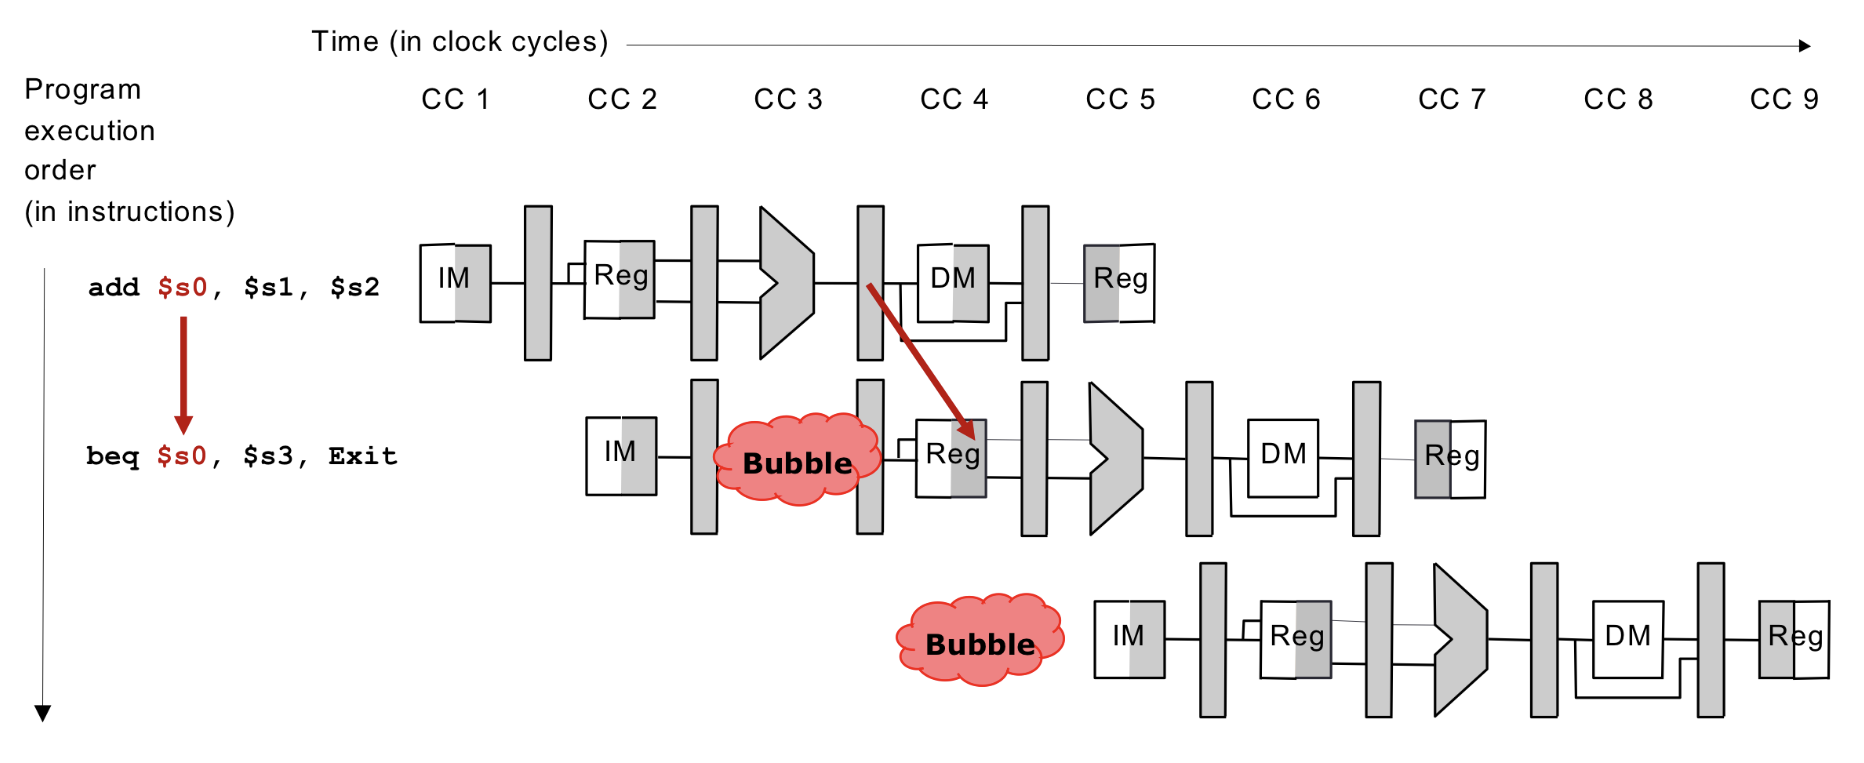
\includegraphics[width=0.49\textwidth]{earlyBranch2}
  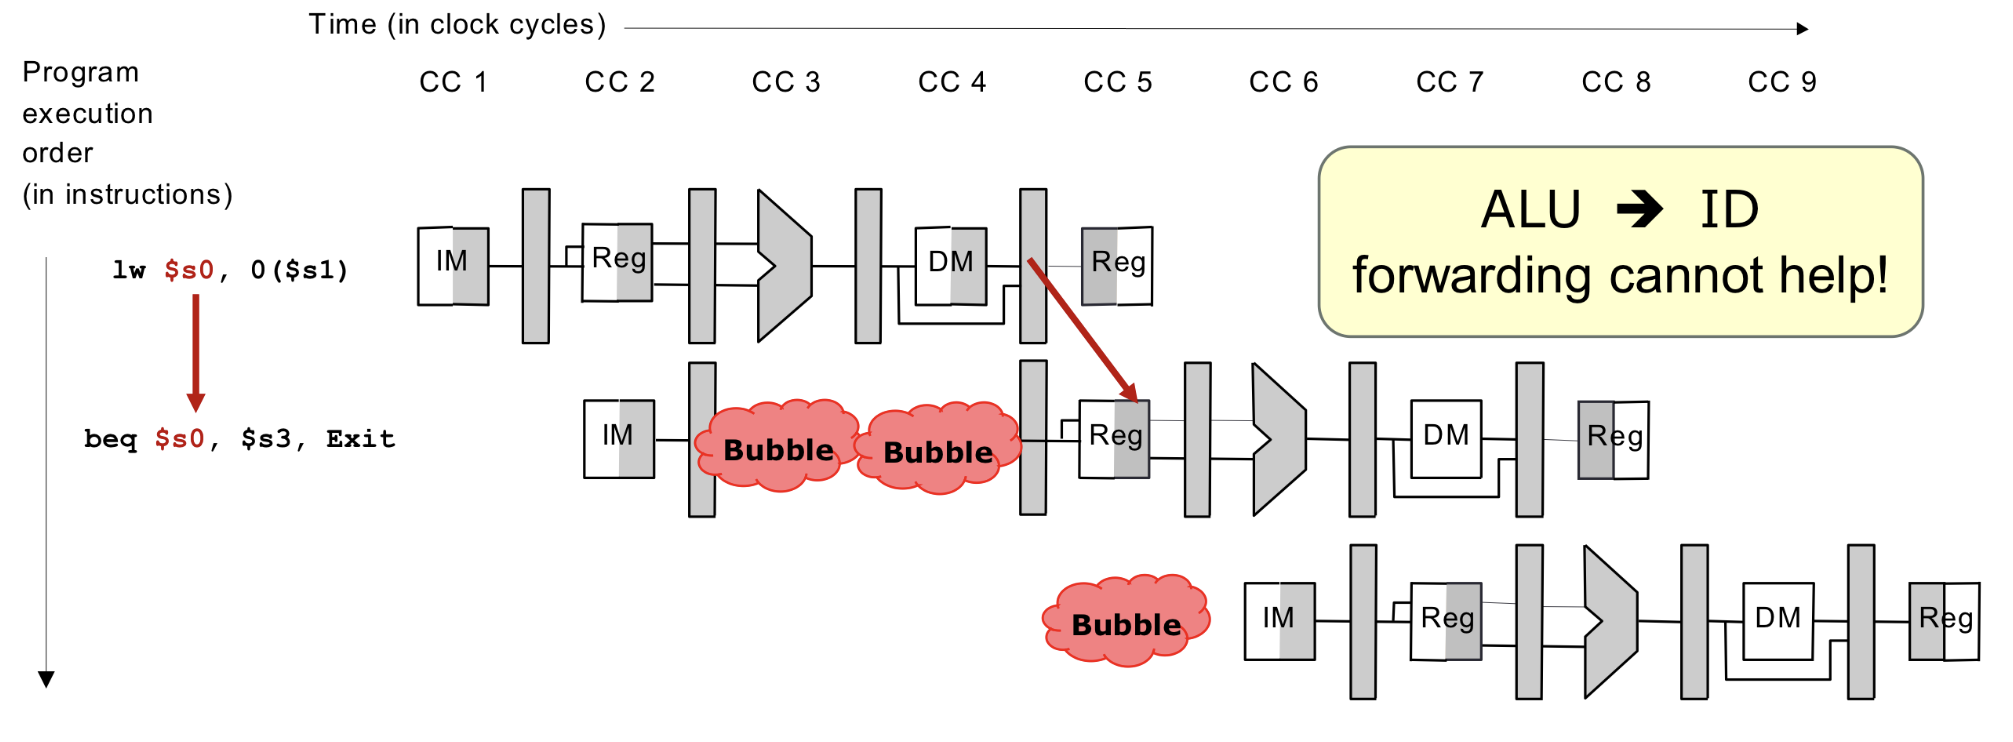
\includegraphics[width=0.5\textwidth]{earlyBranch3}
\end{figure}

\paragraph{Branch Prediction}
We adopt the simple branch prediction scheme of assuming the branch not taken,
and continue ``pumping'' the successor instructions into the pipeline. If the
assumption is true, zero stall is required. If the assumption is false (the
branch is taken), then the piped instructions should not be executed, and are
flushed from the pipeline.

\begin{figure}[h!]
  \centering
  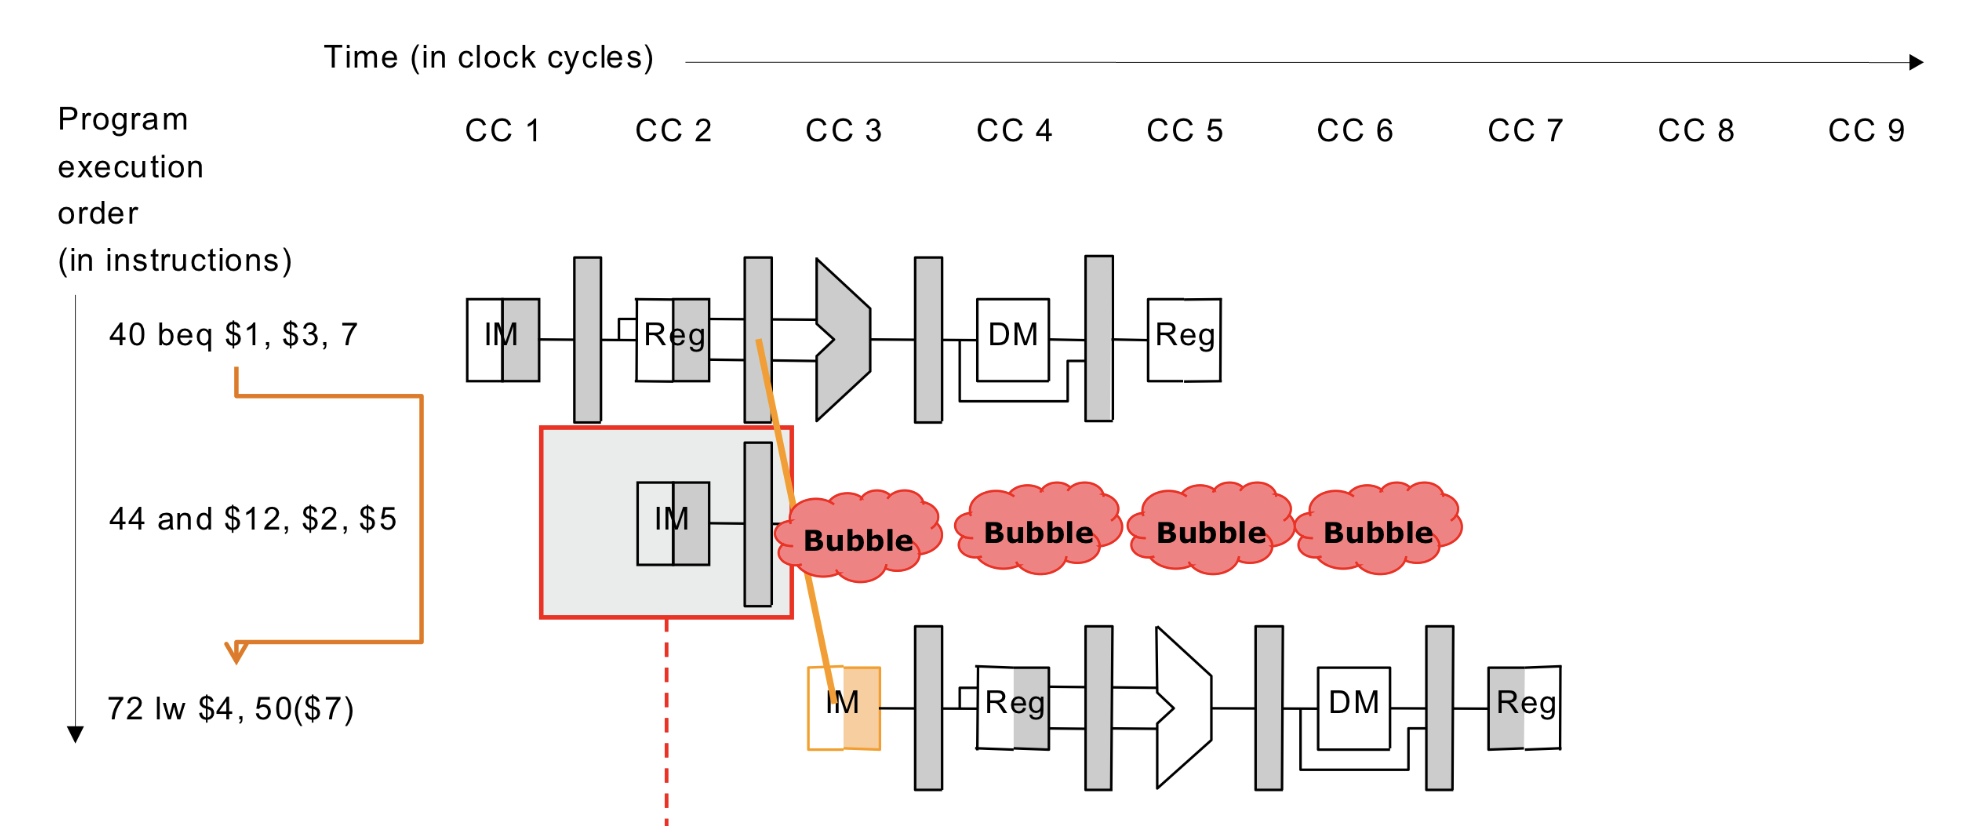
\includegraphics[width=0.6\textwidth]{branchPred}
\end{figure}

If early branching is adopted, this only causes a 1 cycle delay. Otherwise, 3
instructions would have been ``pumped'' and introduces a 3 cycle delay.

\paragraph{Delayed Branch}
To make use of the cycles that a branch might stall on, we may move non-control
dependent instructions that are executed regardless of the branch outcome.

\begin{multicols}{2}
  \begin{lstlisting}
    or  $8, $9, $10 // Non-control dependent
    add $1, $2, $3
    sub $4, $5, $6
    beq $1, $4, Exit
    xor $10, $1, $11

  Exit:
  \end{lstlisting}
  \begin{lstlisting}
    add $1, $2, $3
    sub $4, $5, $6
    beq $1, $4, Exit
    or  $8, $9, $10 // Branch-Delay Slot
    xor $10, $1, $11

  Exit:
  \end{lstlisting}
\end{multicols}

In MIPS, we have 1 branch-delay slot (with early branching). If there is no
such instruction that can be moved while preserving program correctness, a
\verb|nop| instruction is added.

\section{Cache}
Currently, the dominant memory technology in the PC market is the Double Data
Rate-Synchronous Dynamic RAM, delivering memory on both the positive and
negative edge of the clock.
\begin{example}[DDR5]
  The DDR5 Generation delivers information at a rate of
  \[MemClkFreq \times 2^{5} \times 8 \text{ words}.\] 
\end{example}
The technologies of our processors and ICs have been increasing exponentially,
introducing a gap with the performance of the DRAMs. This necessitates the
utilisation of faster memory technology such as SRAM (with lower density and
higher costs, but faster access latency).
\begin{figure}[h!]
  \centering
  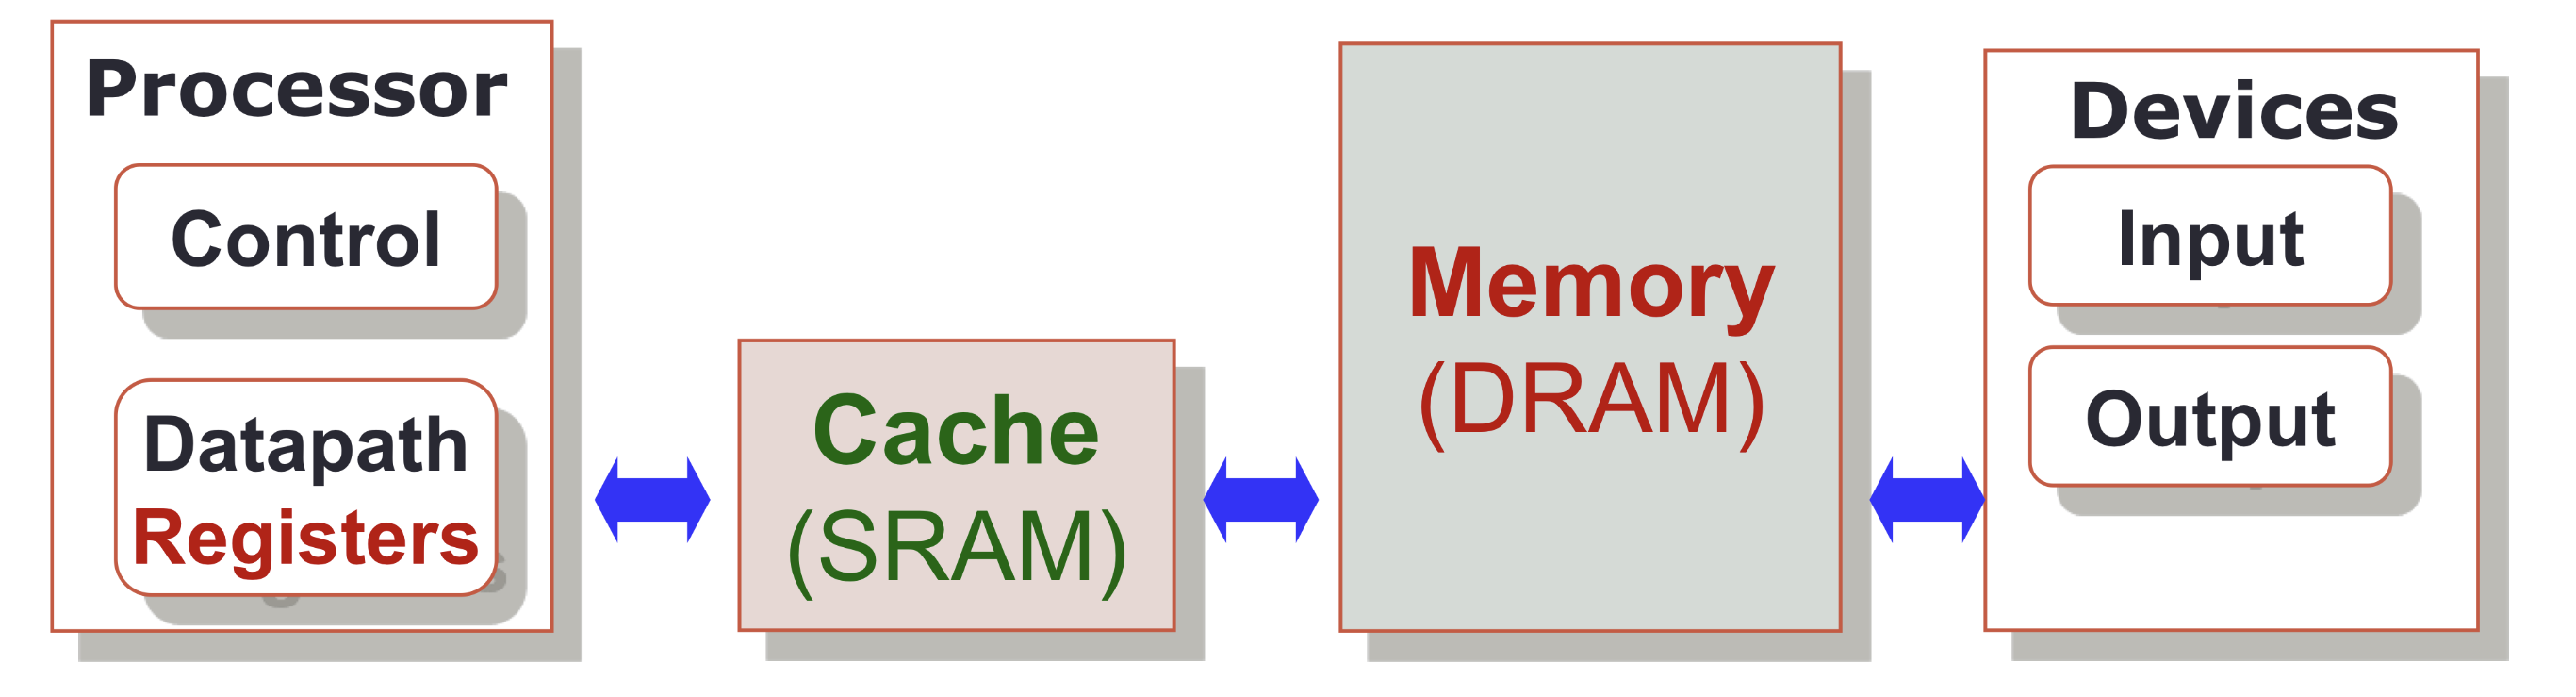
\includegraphics[width=0.5\textwidth]{memories2}
  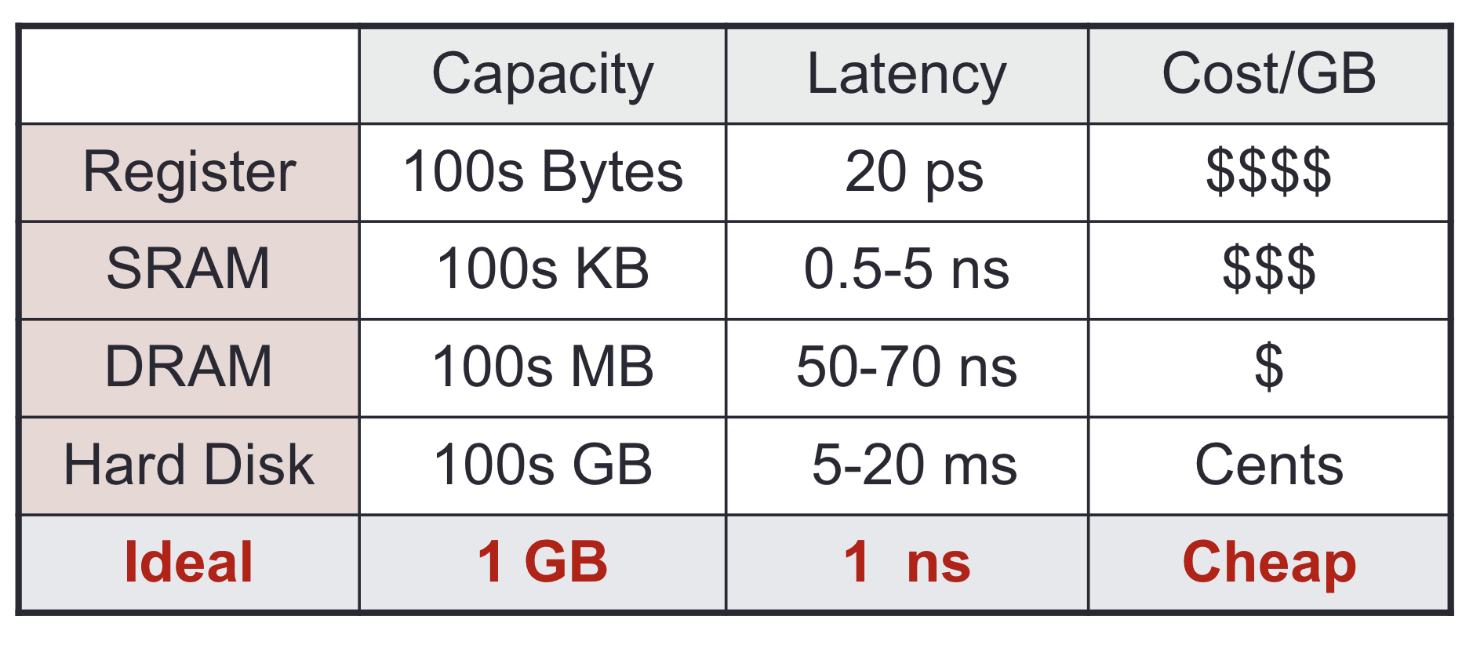
\includegraphics[width=0.4\textwidth]{memories}
\end{figure}

To simulate a large and fast access memory, we use a hierachy of memory
technologies,to keep frequently and recently used data in a smaller but fast
memory and refer to the larger and slower memory only if needed.

\paragraph{Principle of Locality} This is effective as programs access only a
small portion of the memory address space within a small time interval.
\begin{figure}[h!]
  \centering
  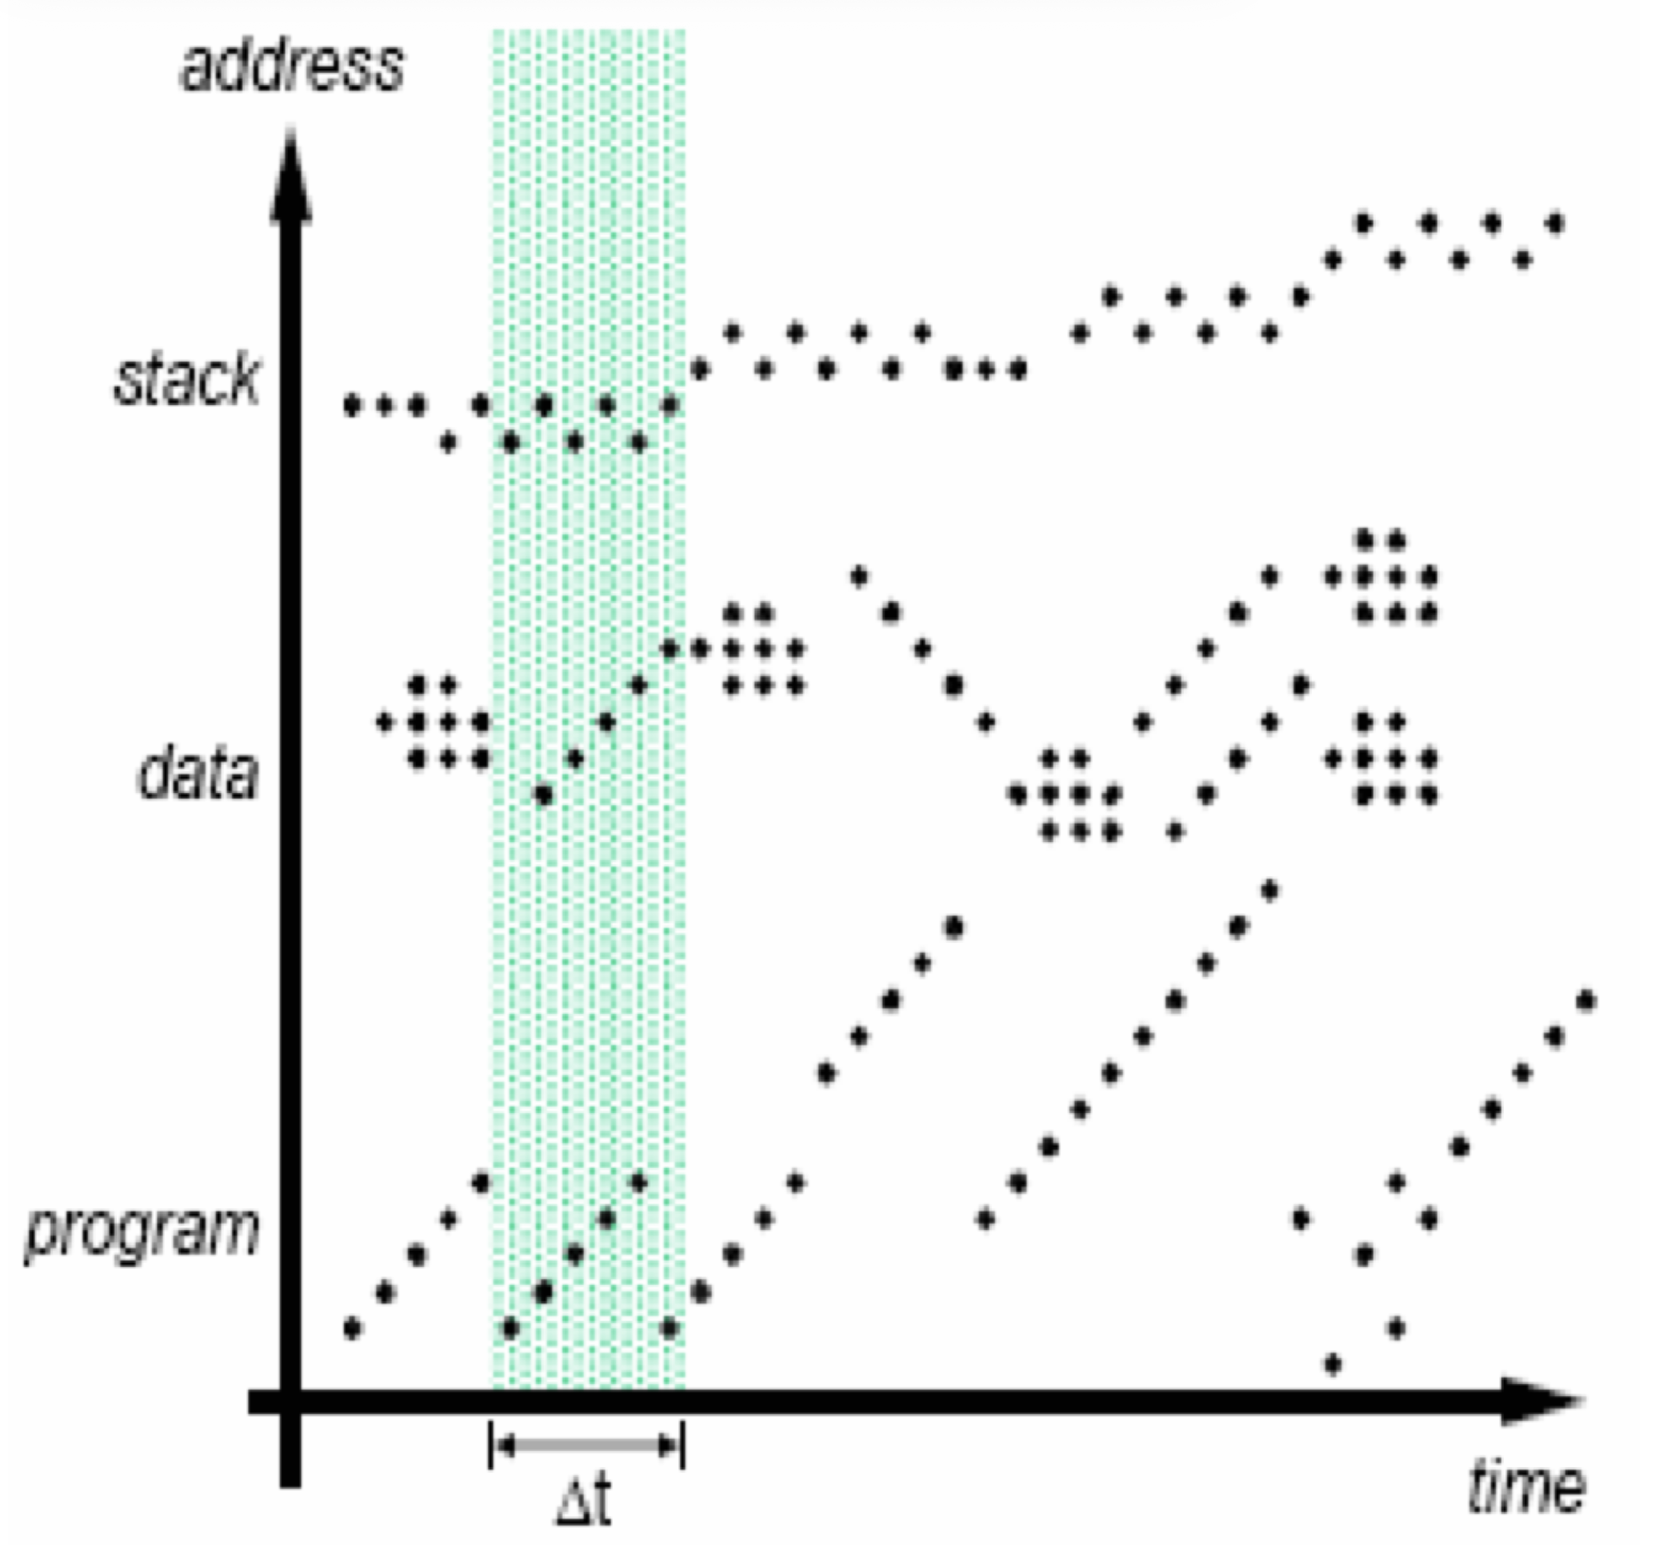
\includegraphics[width=0.3\textwidth]{workingSet}
\end{figure}
\begin{itemize}
  \item \textbf{Temporal Locality}: When an item is referenced, it tends to be
    referenced again. This applies for many programs involving loops.
  \item \textbf{Spatial Locality}: When an item is referenced, nearby items
    tend to be referenced as well. This especially applies to certain data
    structures, particularly arrays and instructions.
\end{itemize}

\begin{definition}[Working Set]
  A working set is a set of locations accessed during some $\Delta t$.
\end{definition}
We may use different working sets during different phases of execution, and we
aim to capture the working set to keep in memory with fastest access latencies.
We do so by creating a cache that is hardware managed.

We now investigate various implementations of mappings betweeen the memory and
the cache.

\begin{definition}[Cache Blocks/Lines]
  A \textit{cache block} is a unit of transfer between the memory and cache,
  typically consisting more than one word, to take advantage of spatial locality.
\end{definition}
\begin{figure}[h!]
  \centering
  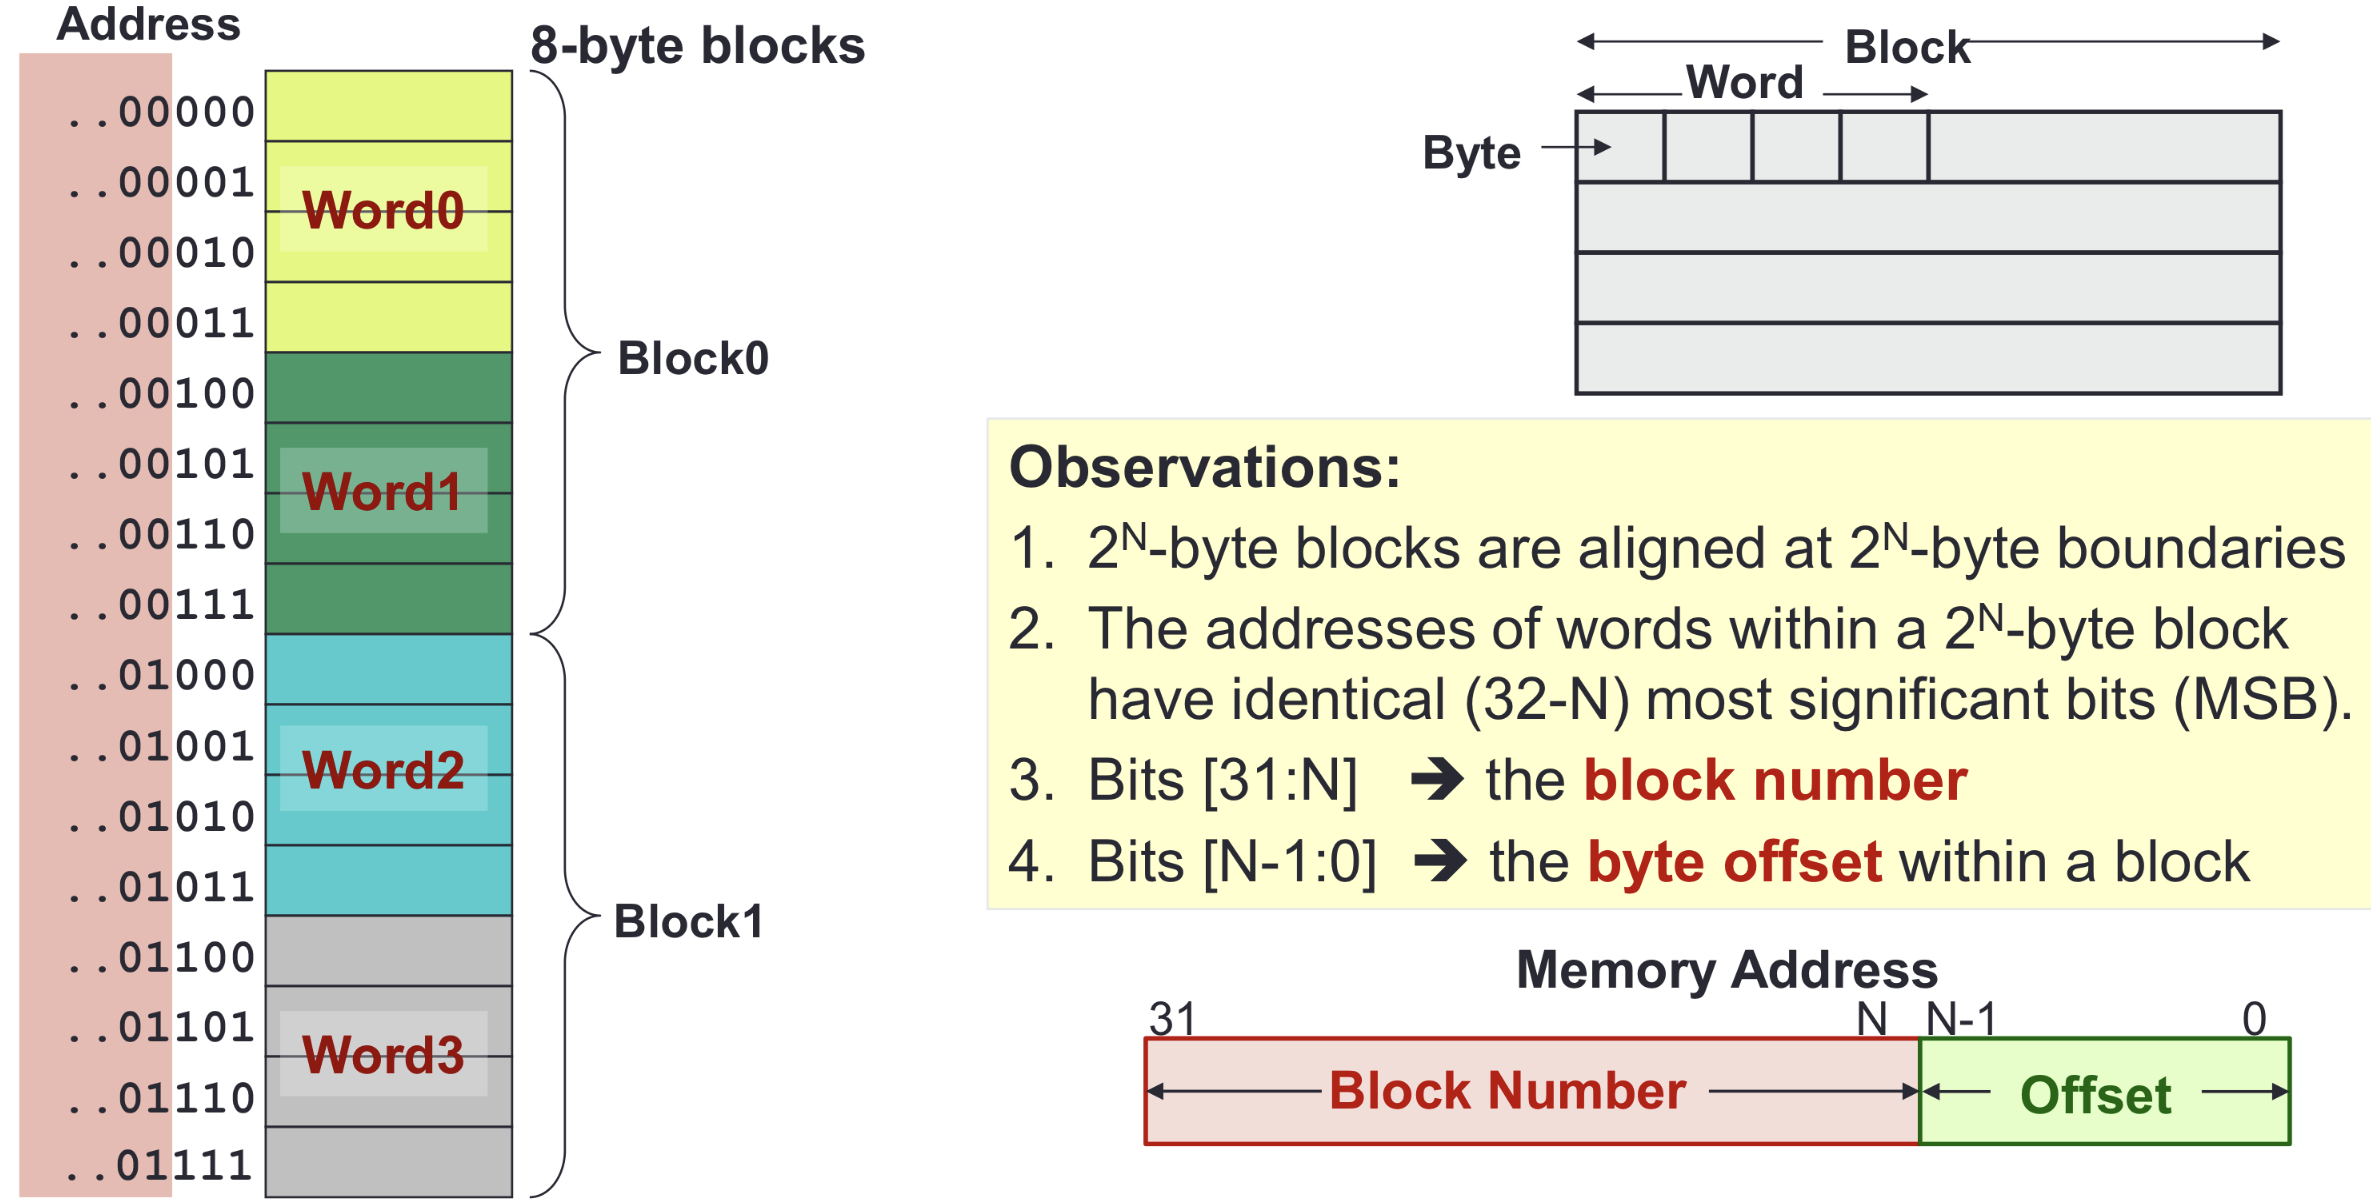
\includegraphics[width=0.6\textwidth]{cache_block}
\end{figure}

\subsection{Cache Misses}
A cache miss occurs due to one of three reasons:
\begin{itemize}
  \item \textbf{Compulsory Miss} (Cold Start Miss / First Reference Miss)
    occurs on first access to the block. The block must be brought into the
    cache.
  \item \textbf{Conflict Miss} (Collision Miss / Interference Miss) occurs in
    the case of directed mapped cache or set associative cache, when several
    blocks are mapped to the same block or set, and it is not a compulsory
    miss.
  \item \textbf{Capacity Miss} occurs when blocks were discarded as the cache
    cannot contain all blocks requested.
\end{itemize}

\subsection{Memory Access}
When a memory address is specified, the data is either in the cache, or not.
\begin{definition}[Cache Hit]
  A \textit{cache hit} occurs when the data is in the cache. We call the fraction
  of memory accesses that hit the \textit{hit rate}, and the time to access
  the cache the \textit{hit time}.
\end{definition}
\begin{definition}[Cache Miss]
  A \textit{cache miss} occurs when the data is not in the cache. We call
  the fraction of memory accesses that miss the \textit{miss rate}$=1-$ hit
  rate, and the time to replace the cache block and then to access the cache
  the  \textit{miss penalty}.
\end{definition}

The average access time is hence obtained by
\[Average\ Access\ Time= Hit\ Rate \times Hit\ Time + Miss\ Rate \times Miss\
Penalty.\] 

\paragraph{Block Size Trade-off}
\begin{figure}[h!]
  \centering
  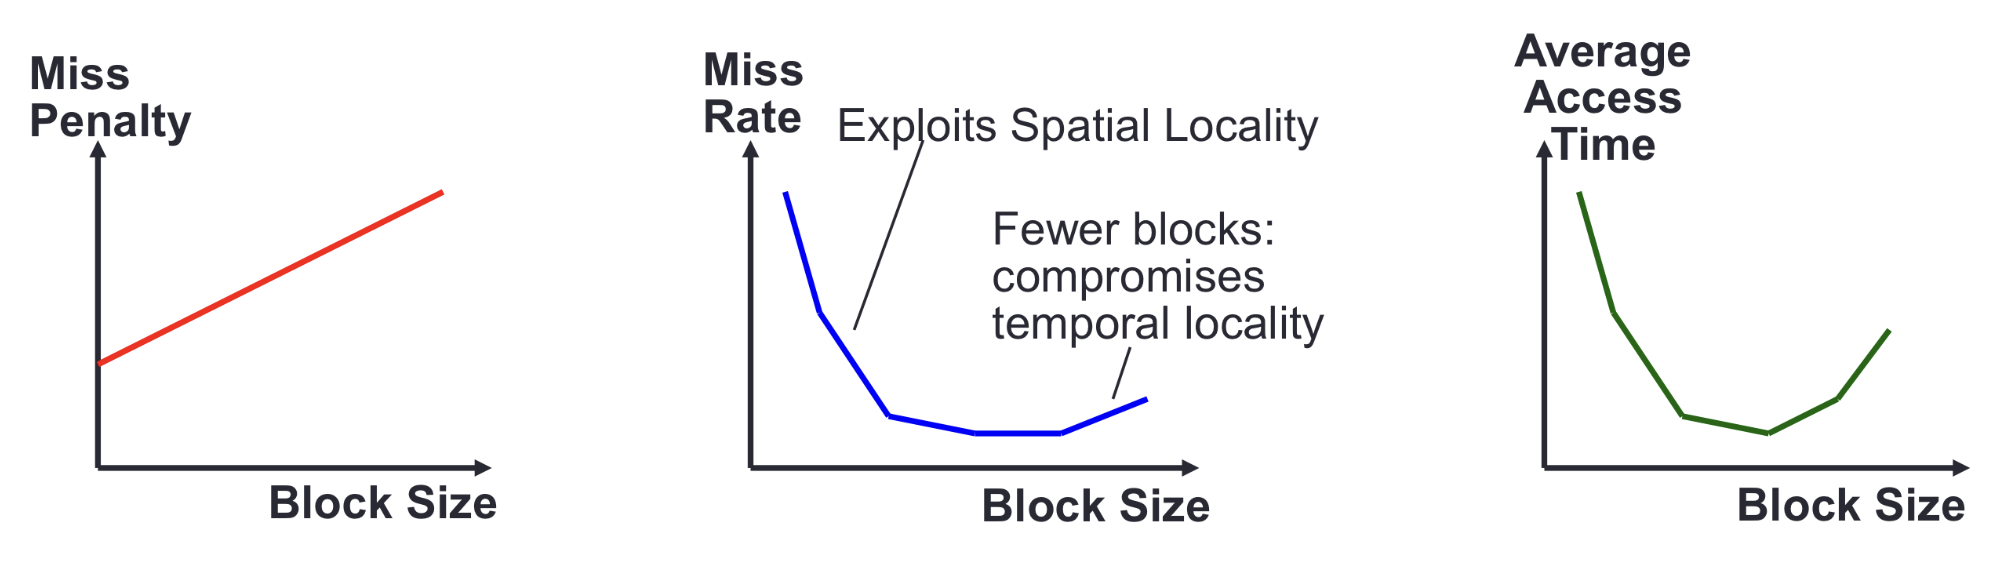
\includegraphics[width=0.6\textwidth]{blockTrade}
\end{figure}
With a larger block size:
\begin{itemize}
  \item Take advantage of spatial locality
  \item Larger miss penalty, requiring longer time to fill up the block
  \item Block size too large relative to cache size results in too few cache
    blocks, increasing miss rate
\end{itemize}

\subsubsection{Reading Data}
On reading data, we first check the cache for the existence of the data block.
If there is a cache miss, we request the data from the main memory, write into
the cache, and then load from the cache to the register.
\begin{figure}[h!]
  \centering
  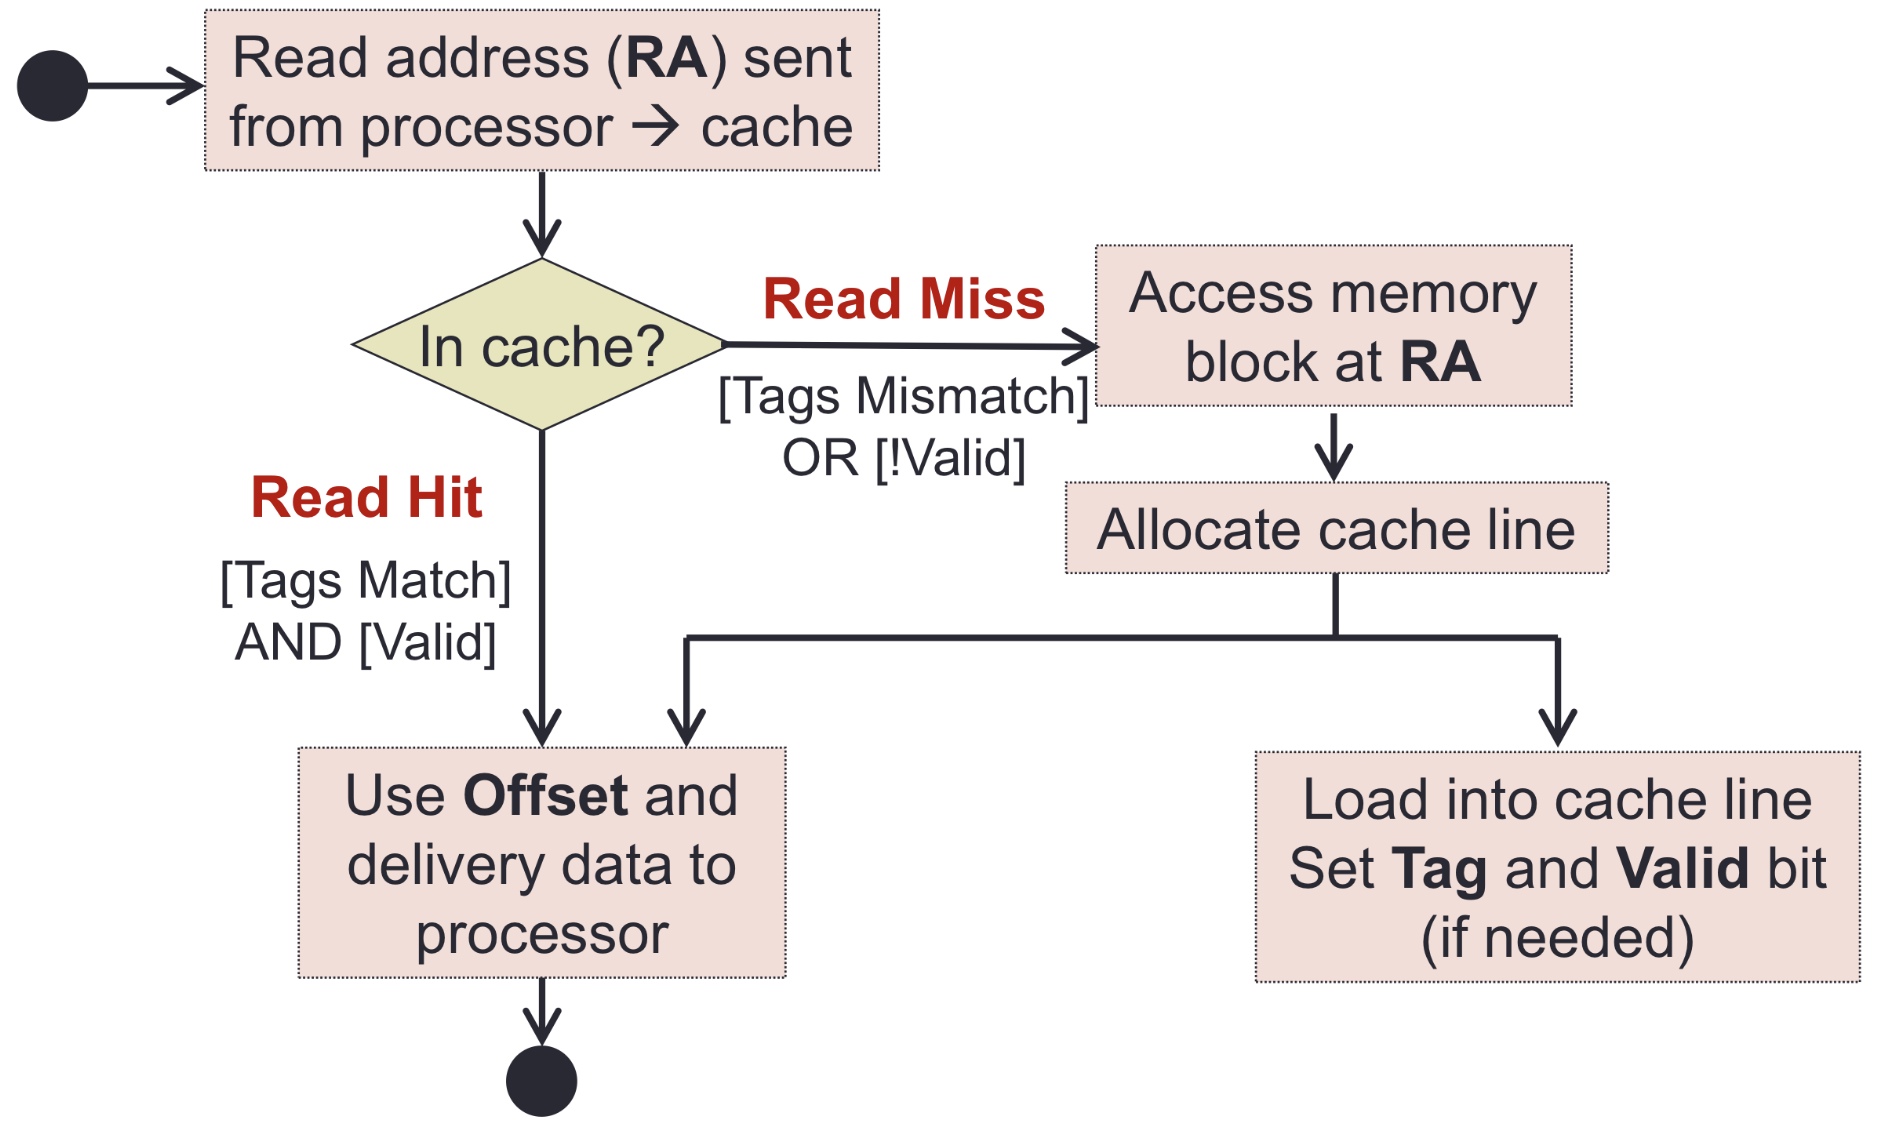
\includegraphics[width=0.5\textwidth]{cacheRead}
\end{figure}

\subsubsection{Writing Data}
On writing data, in case of a \textbf{cache hit}, we must maintain consistency
between the cache and main memory. As such, we have the write policies:
\begin{enumerate}
  \item \textbf{Write-Through Cache}: Write data to both the cache and main
    memory. We add a write buffer between the cache and main-memory, that is
    operated by a memory controller to allow for processor to operate at the
    speed of the cache and write buffer instead of the main memory.
    \begin{figure}[h!]
      \centering
      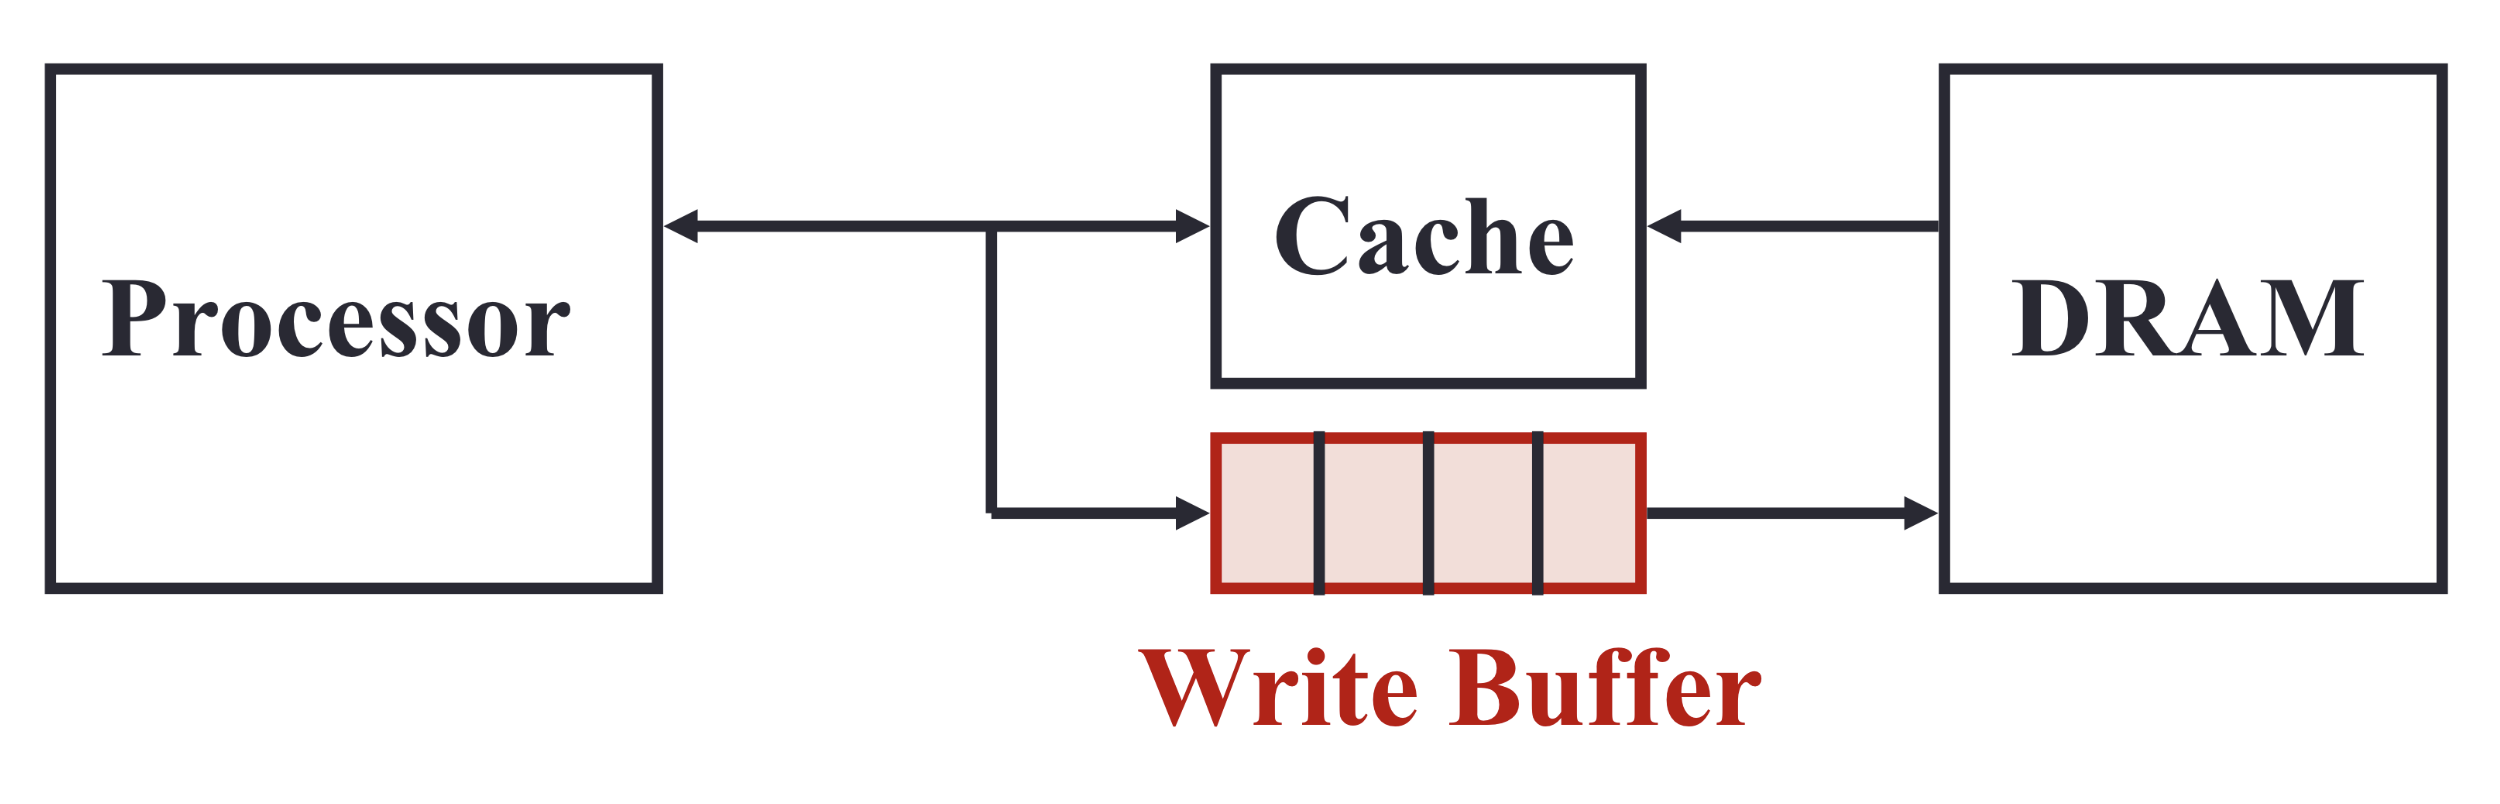
\includegraphics[width=0.4\textwidth]{write_through}
    \end{figure}
    \vspace{-4mm}
  \item \textbf{Write-Back Cache}: Write data to only cache. Commit to memory
    only when the cache block is replaced. We add an additional (Dirty) bit to
    each cache block, to indicate if the cache block has been modified. We only
    attempt to write back to memory when the cache block is being evicted, and
    its dirty bit is 1.
\end{enumerate}

In case of a \textbf{cache miss}, we have the write miss policies:
\begin{enumerate}
  \item \textbf{Write Allocate}: Load the complete block into the cache, change
    only the required word in the cache, and write to main memory depending on
    write policy.
  \item \textbf{Write Around}: Write directly to main memory only.
\end{enumerate}

\begin{figure}[h!]
  \centering
  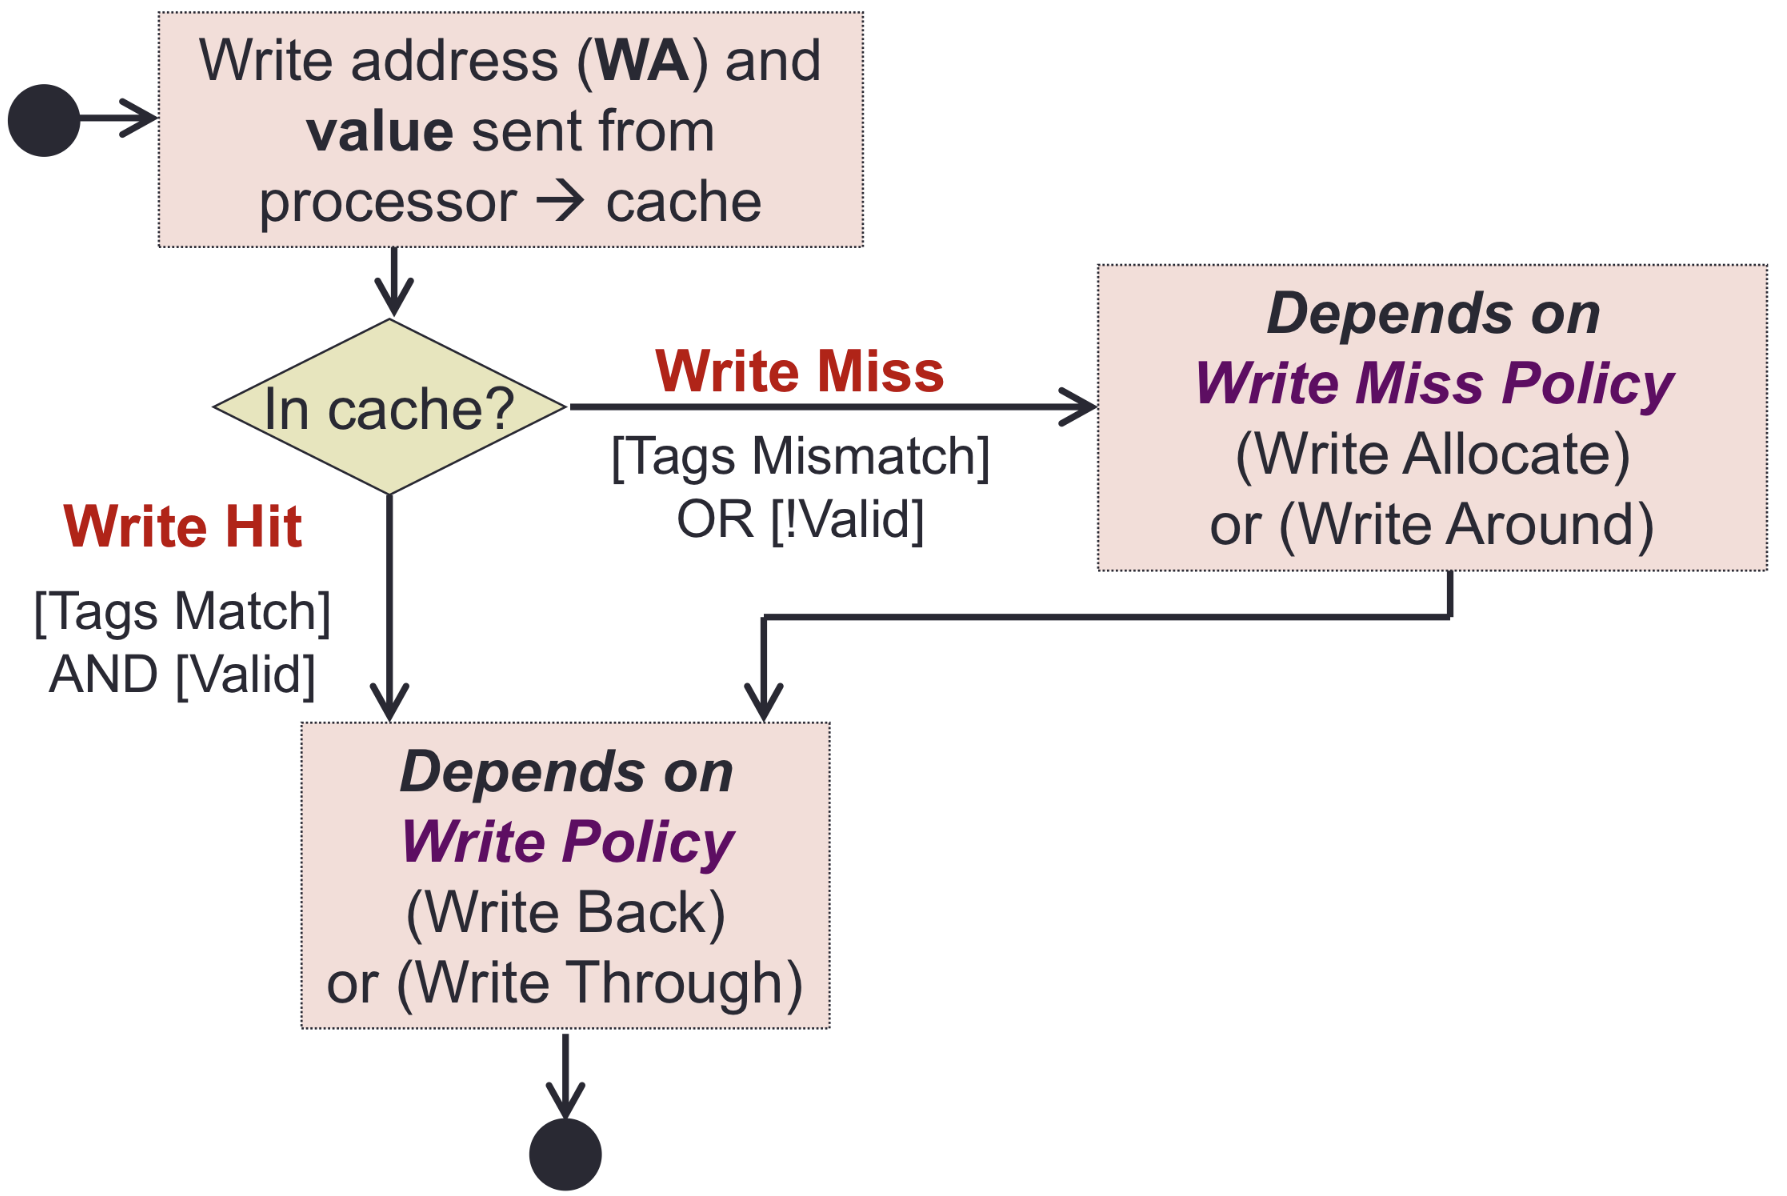
\includegraphics[width=0.5\textwidth]{cacheWrite}
\end{figure}

\subsection{Direct Mapped Cache}
In the Direct Mapped Cache, we identify the next LSBs after
the byte offsets as the \textit{cache index}, which identifies the line in the
cache where this block can be stored. Since multiple blocks in memory can have
the same cache index, we further specific the address with the \textit{tag},
the rest of the bits in the memory address and we have a mapping from the main
memory to the cache.
\[Cache\ Index=(Block\ Number) \bmod (Number\ of\ Cache\ Blocks).\] 
\[Tag=(Block\ Number) / (Number\ of\ Cache\ Blocks).\] 
\begin{figure}[h!]
  \centering
  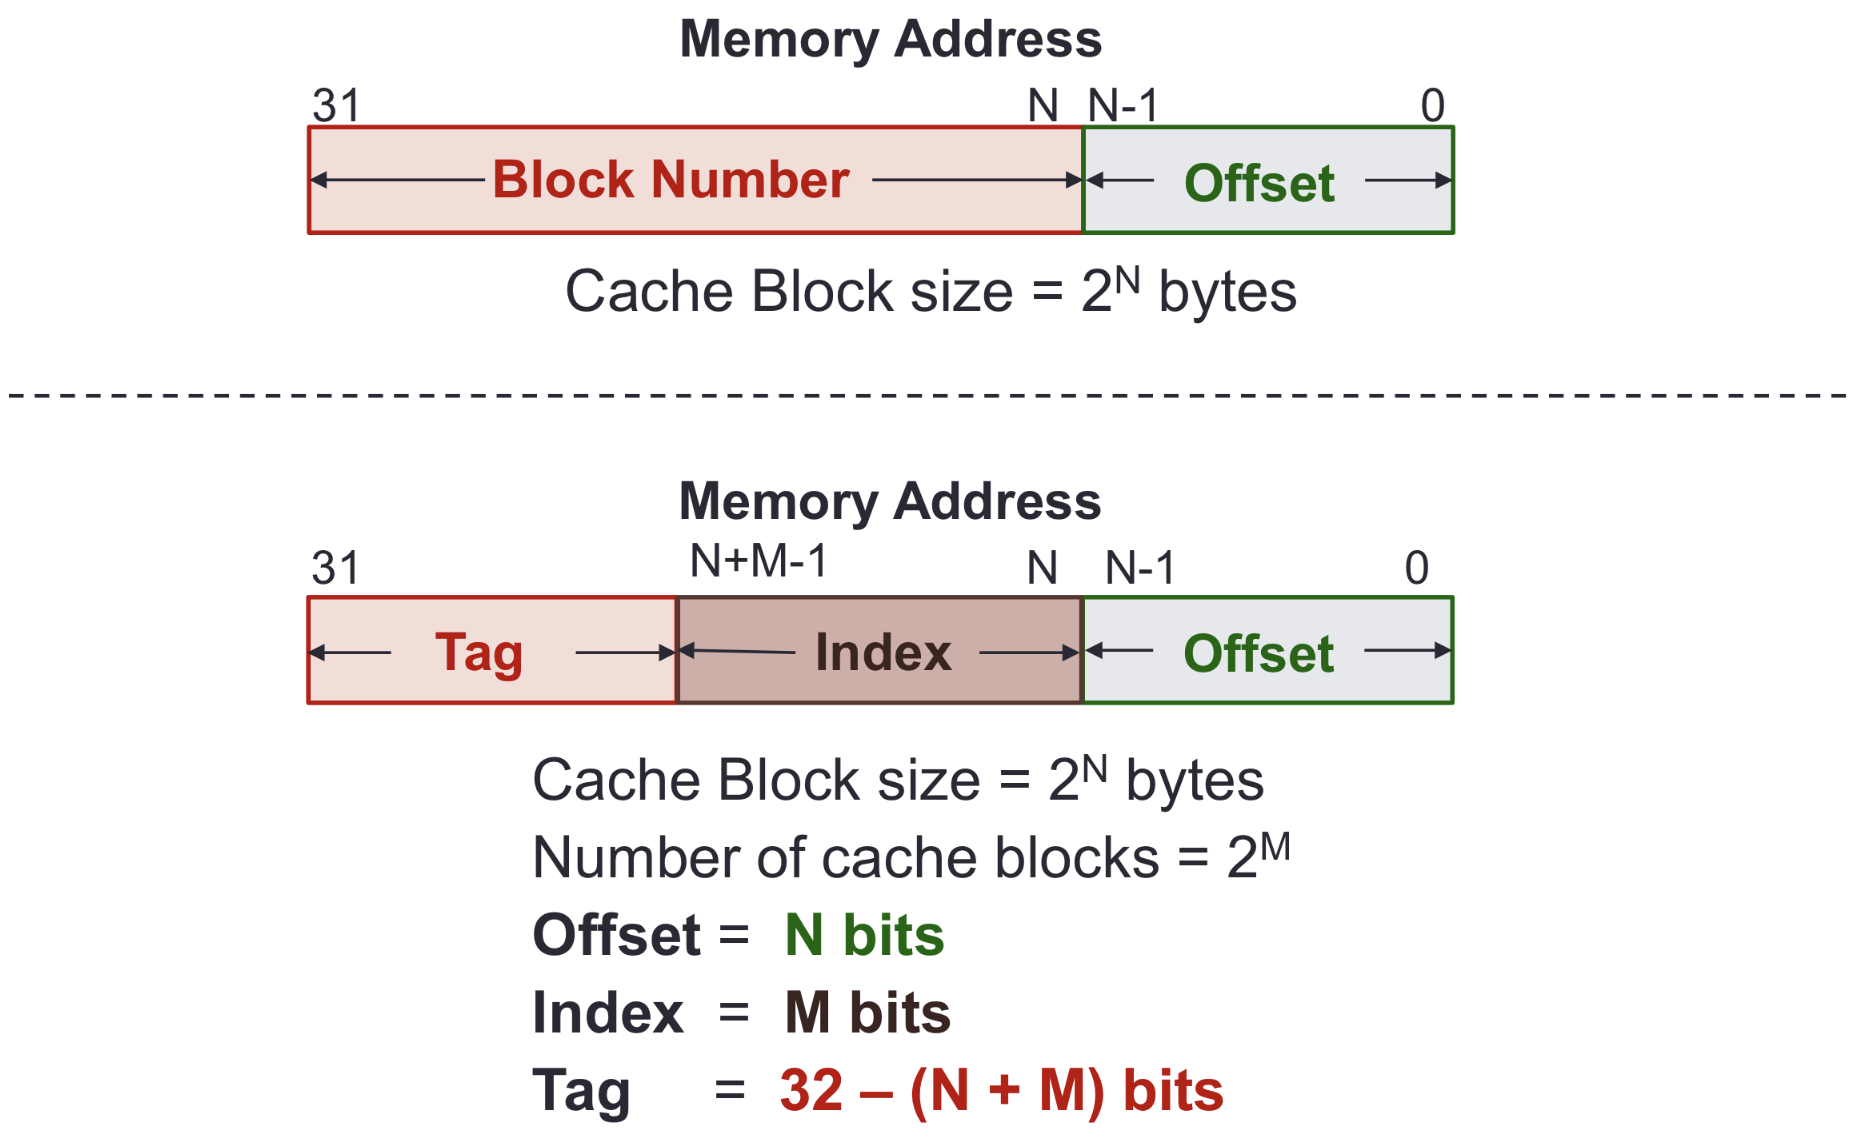
\includegraphics[width=0.55\textwidth]{dmc_map}
\end{figure}\\
The cache hence consists of the following components for each block:
\begin{itemize}
  \item \textbf{Valid Bit} indicating whether the cache line contains valid data
  \item \textbf{Tag} of the memory block
  \item \textbf{Data Block}
\end{itemize}
Given a memory address, we compute its index and tag, and a cache hit occurs $\iff$
\verb|Valid[index]=TRUE| $\wedge$ \verb|Tag[index]=tag|.
\begin{figure}[h!]
  \centering
  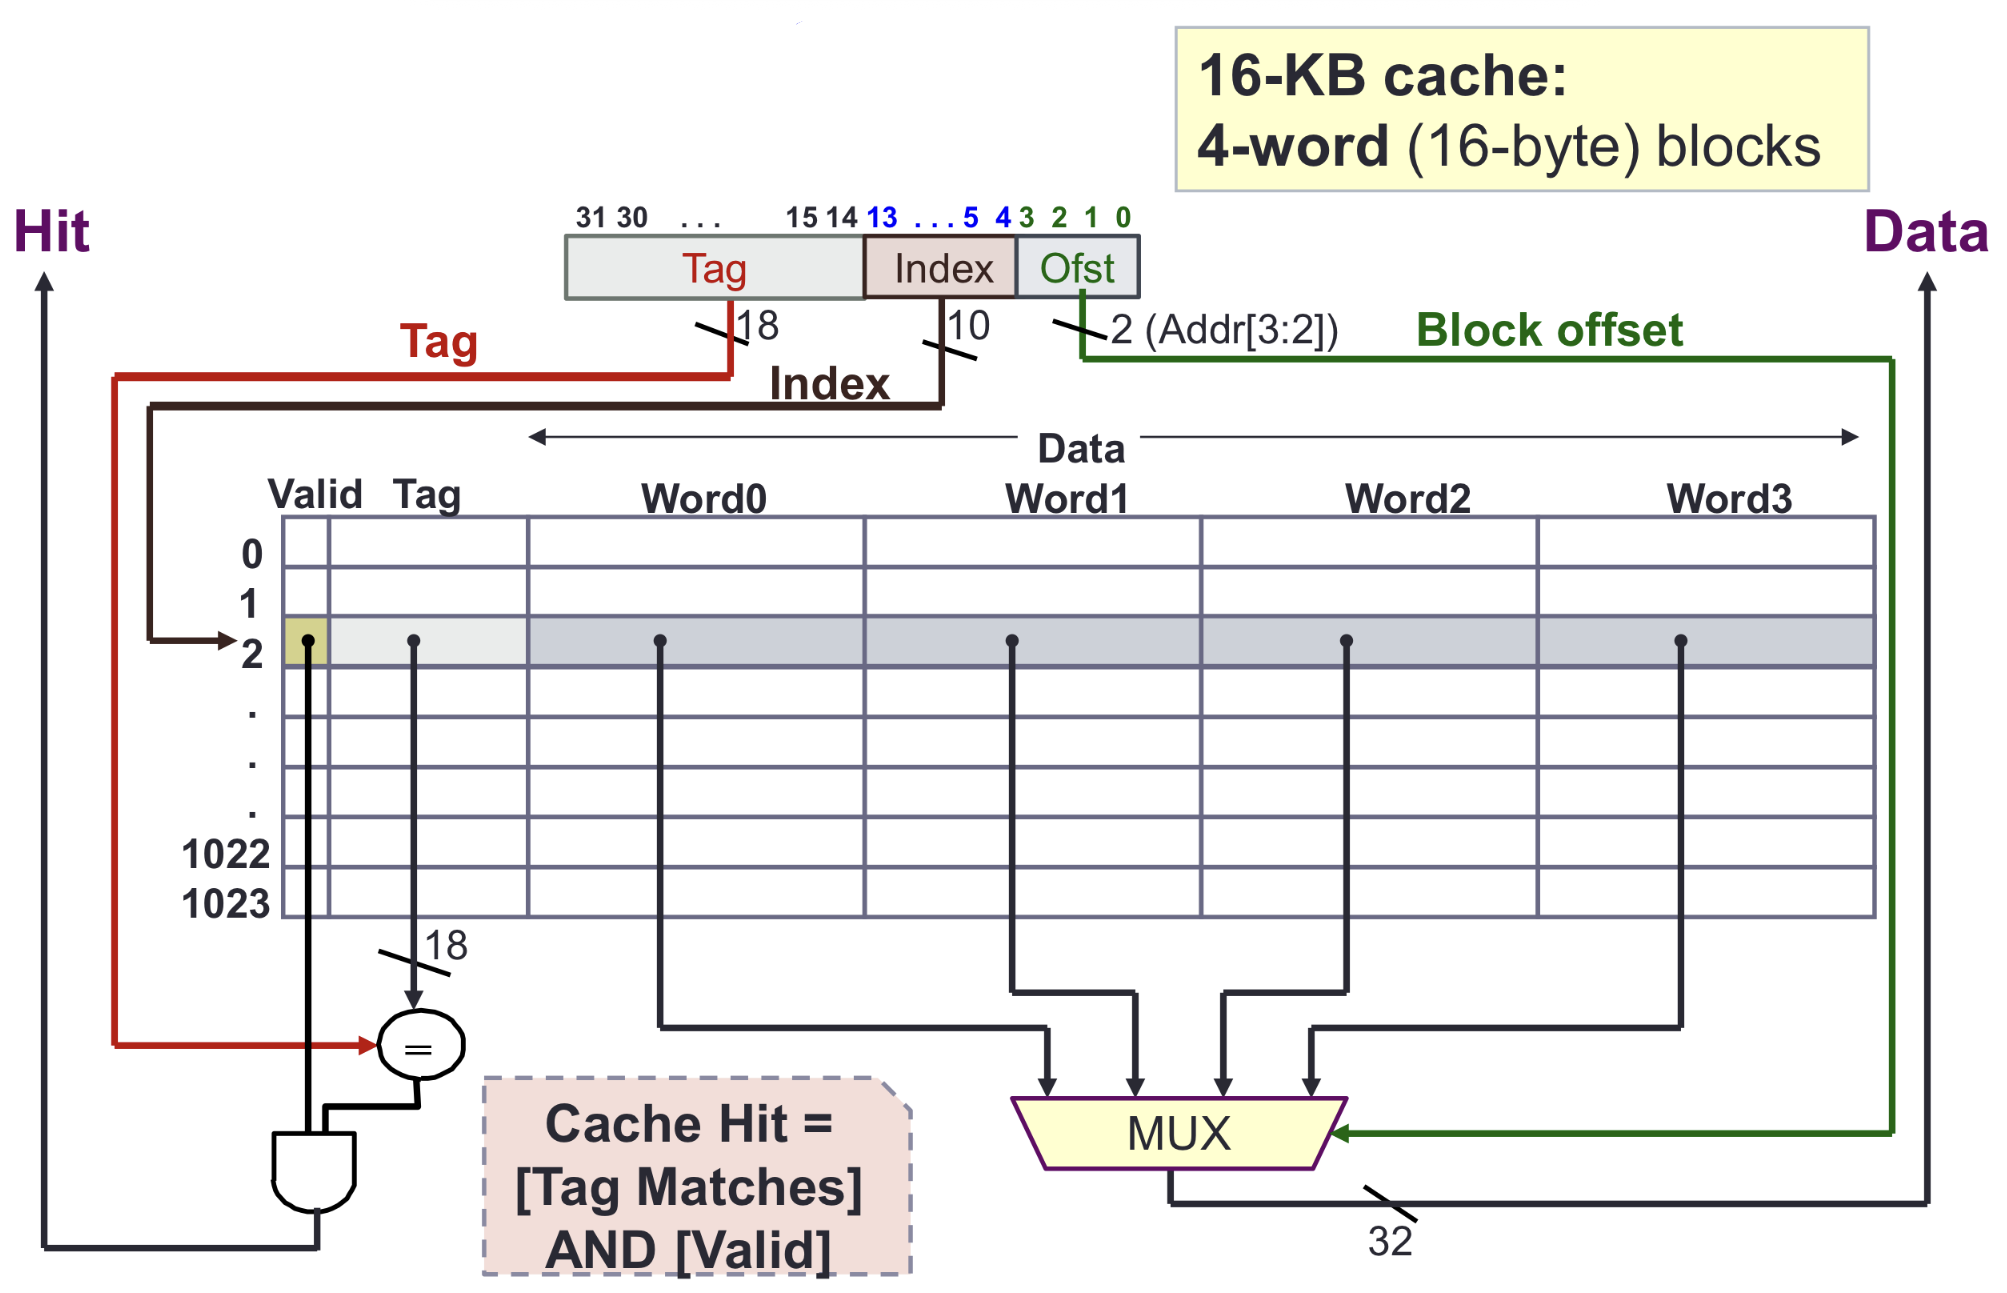
\includegraphics[width=0.5\textwidth]{cacheCircuit}
\end{figure}

\subsection{Set Associative Cache}
In a Set Associative Cache, we attempt to circumvent the issue of conflict
misses. We define a $N$-way Set Associative Cache in which each memory block
can be placed in a fixed number ($N>1$) of locations in the cache. The cache
consists a number of sets, each containing $N$ cache blocks. Each memory block
maps to a unique cache set within which it can be placed in any of the $N$
cache blocks.

\begin{figure}[h!]
  \centering
  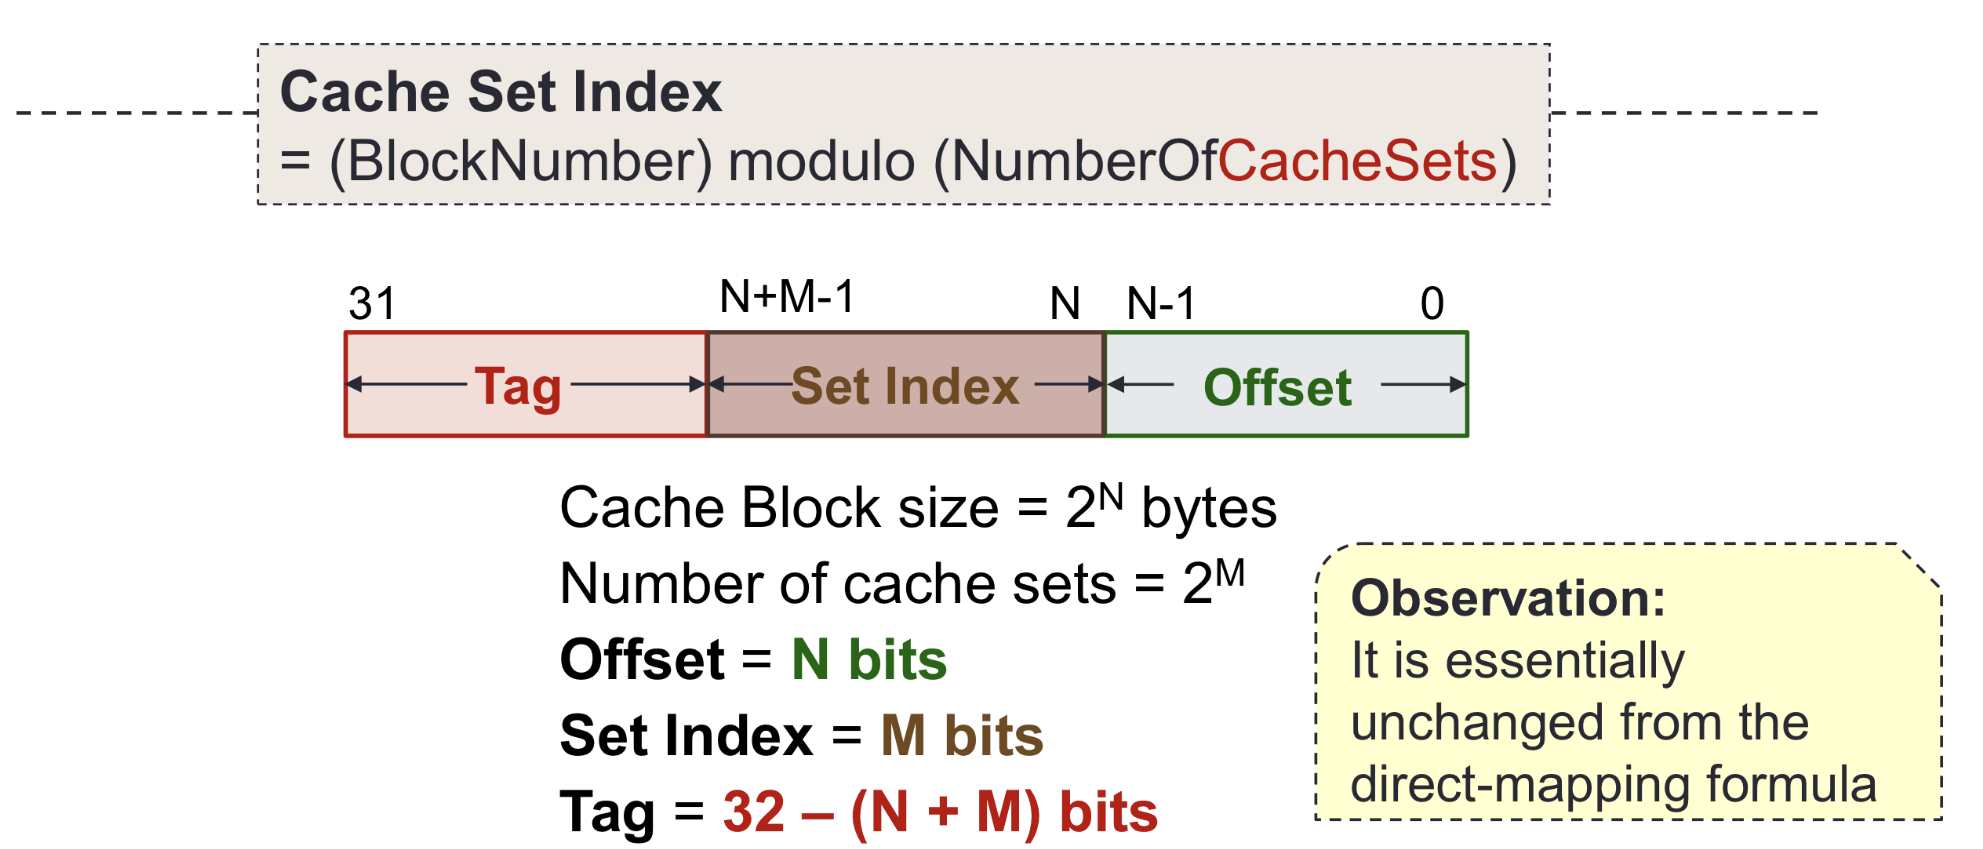
\includegraphics[width=0.6\textwidth]{sacMap}
\end{figure}

\begin{figure}[h!]
  \centering
  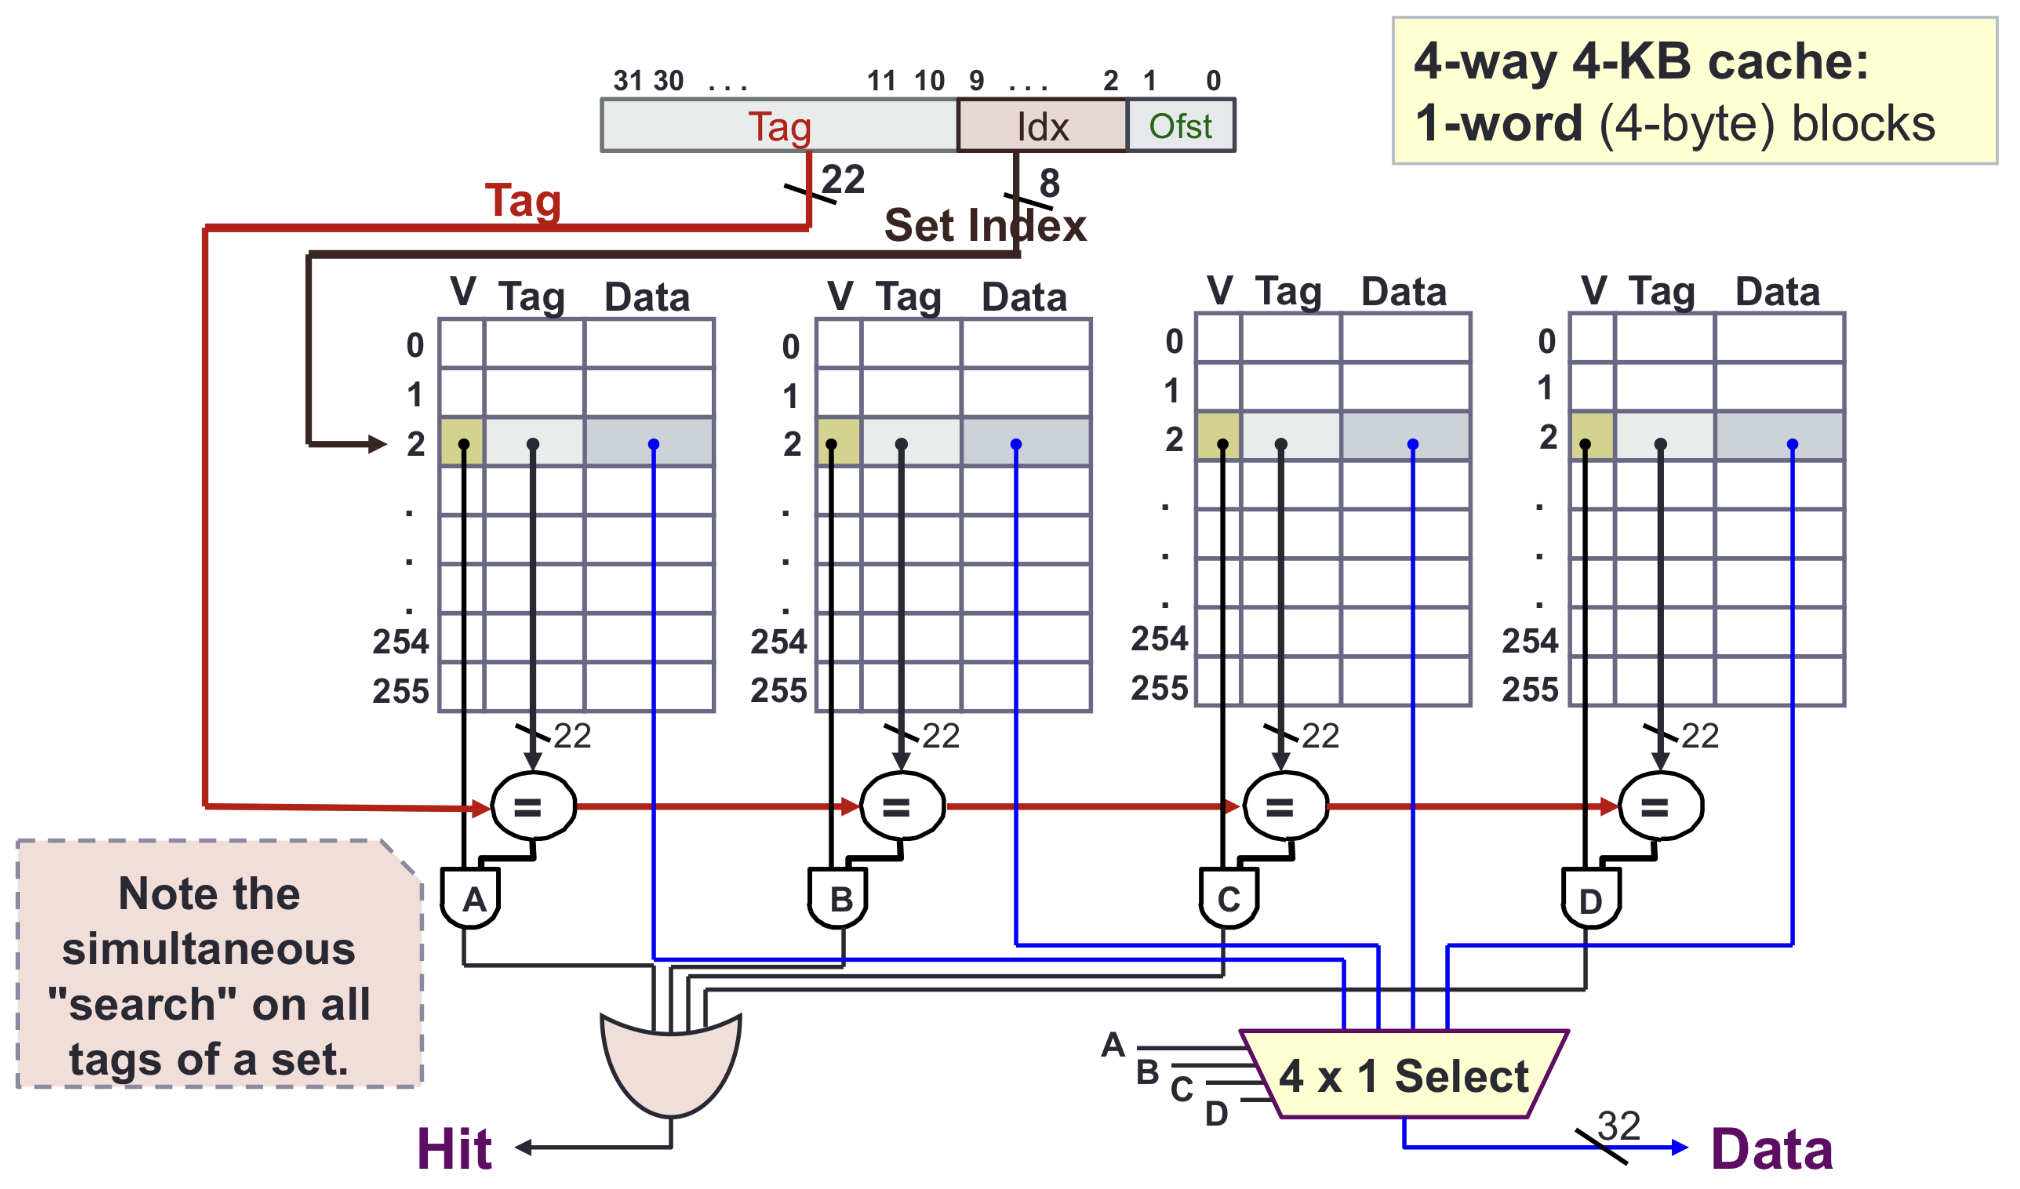
\includegraphics[width=0.65\textwidth]{sacCircuit}
\end{figure}

\begin{prop}[Miss Rate of SAC vs DAC]
  A Direct-Mapped Cache of size $N$ has about the same miss rate as a $2$-way
  Set Associative Cache of size $\frac{N}{2}$.
\end{prop}

\subsubsection{Block Replacement Policy}
When the cache set is full, we have a choice of memory blocks that can be replaced
within the cache set. As such, we may define a block replacement policy:
\begin{itemize}
  \item \textbf{Least Recently Used} (Difficult to keep track if $N$ is large)
  \item \textbf{First In First Out}
  \item \textbf{Random Replacement}
  \item \textbf{Least Frequently Used}
\end{itemize}

\subsection{Fully Associative Cache}
In a Fully Associative Cache, a memory block can be placed in any location in
the cache. This eliminates conflict misses, since blocks are not restricted in
their locations. However, this requires searching all cache blocks for memory
access. Essentially, the entire cache is a cache set for all memory blocks.

\begin{figure}[h!]
  \centering
  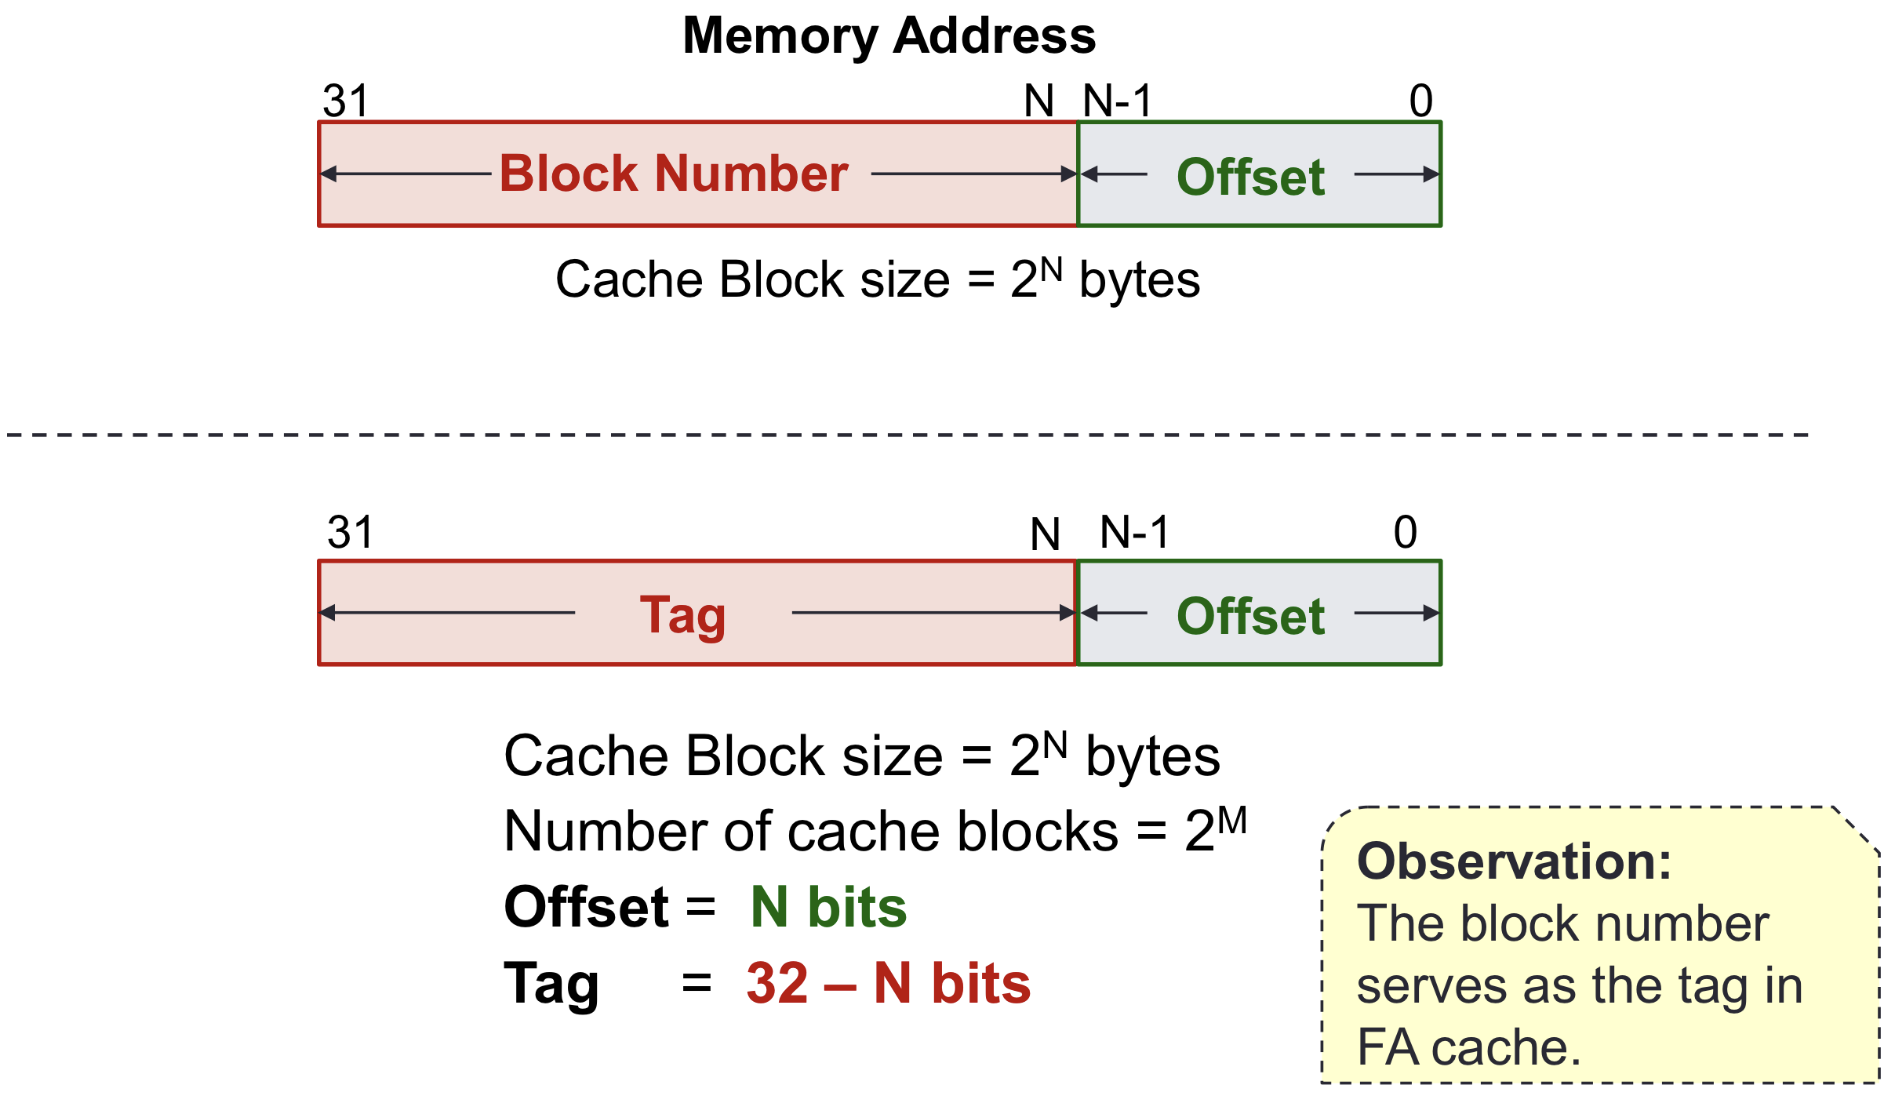
\includegraphics[width=0.55\textwidth]{facmap}
\end{figure}
\begin{figure}[h!]
  \centering
  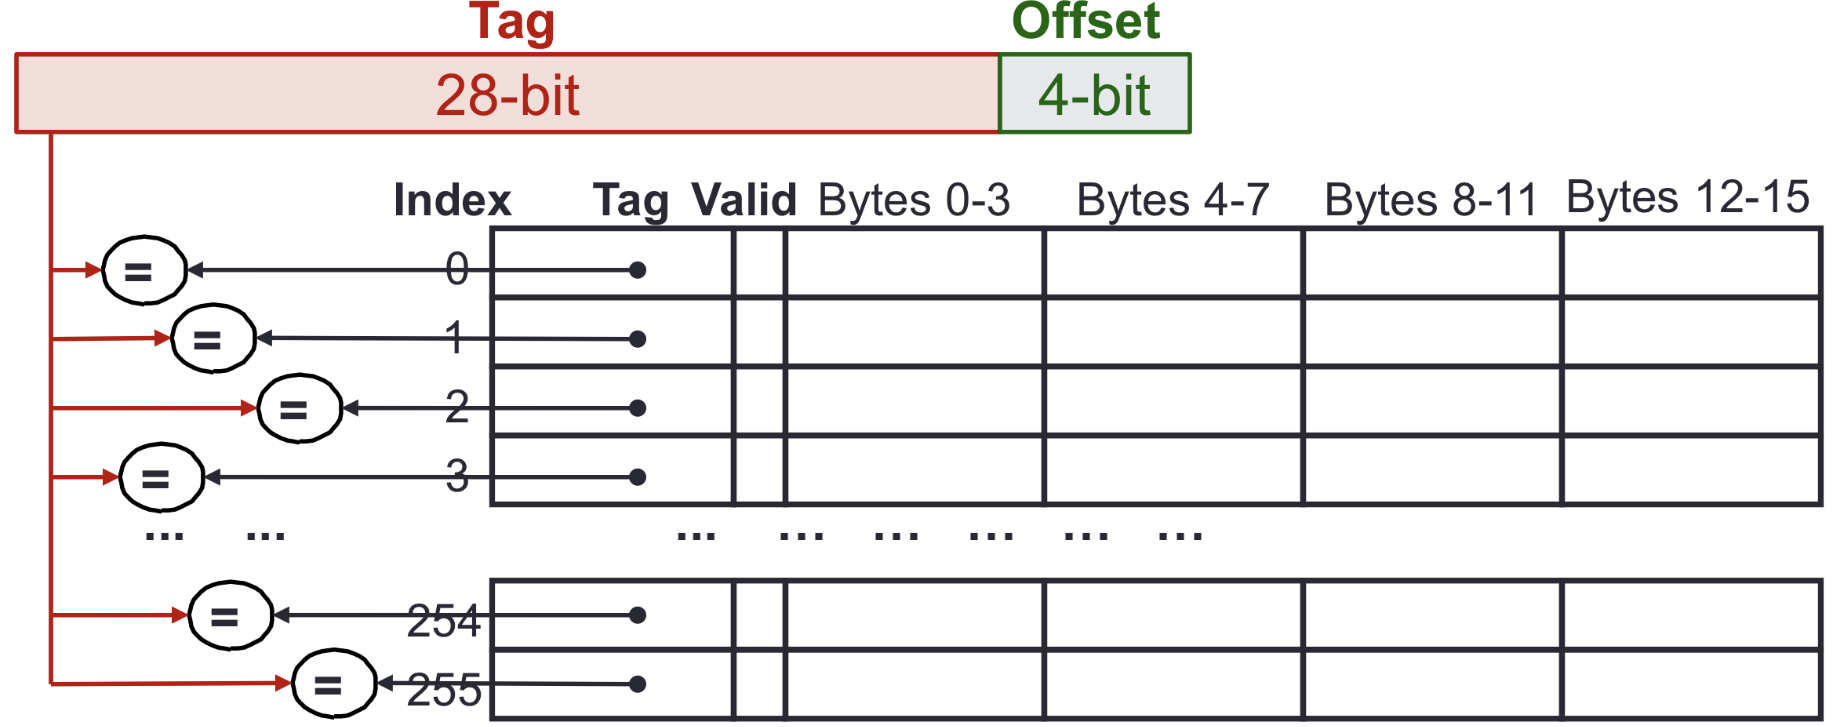
\includegraphics[width=0.6\textwidth]{facCircuit}
\end{figure}

\subsection{Cache Performances Comparisons}
In comparison of cache sizes and associativity, we may derive various trends
that allow us to optimise caches for specific contexts.
\paragraph{Compulsory Misses} remain the same regardless of cache size and
associativity.
\paragraph{Conflict Misses} decreases with increasing associativity, for the
same cache size. It is $0$ for FACs.
\paragraph{Capacity Misses} remain the same regardless of associativity, for
the same cache size. It decreases with increasing cache size.
\[Total\ Miss=Cold\ Miss + Conflict\ Miss + Capacity\ Miss.\] 

\subsection{Multilevel Caches}
To decrease average access times, we may also decrease the miss penalty. One
such method is to consider multilevel caches, to either separate data and
instruction caches (with differing localities) or a unified cache.

\begin{figure}[h!]
  \centering
  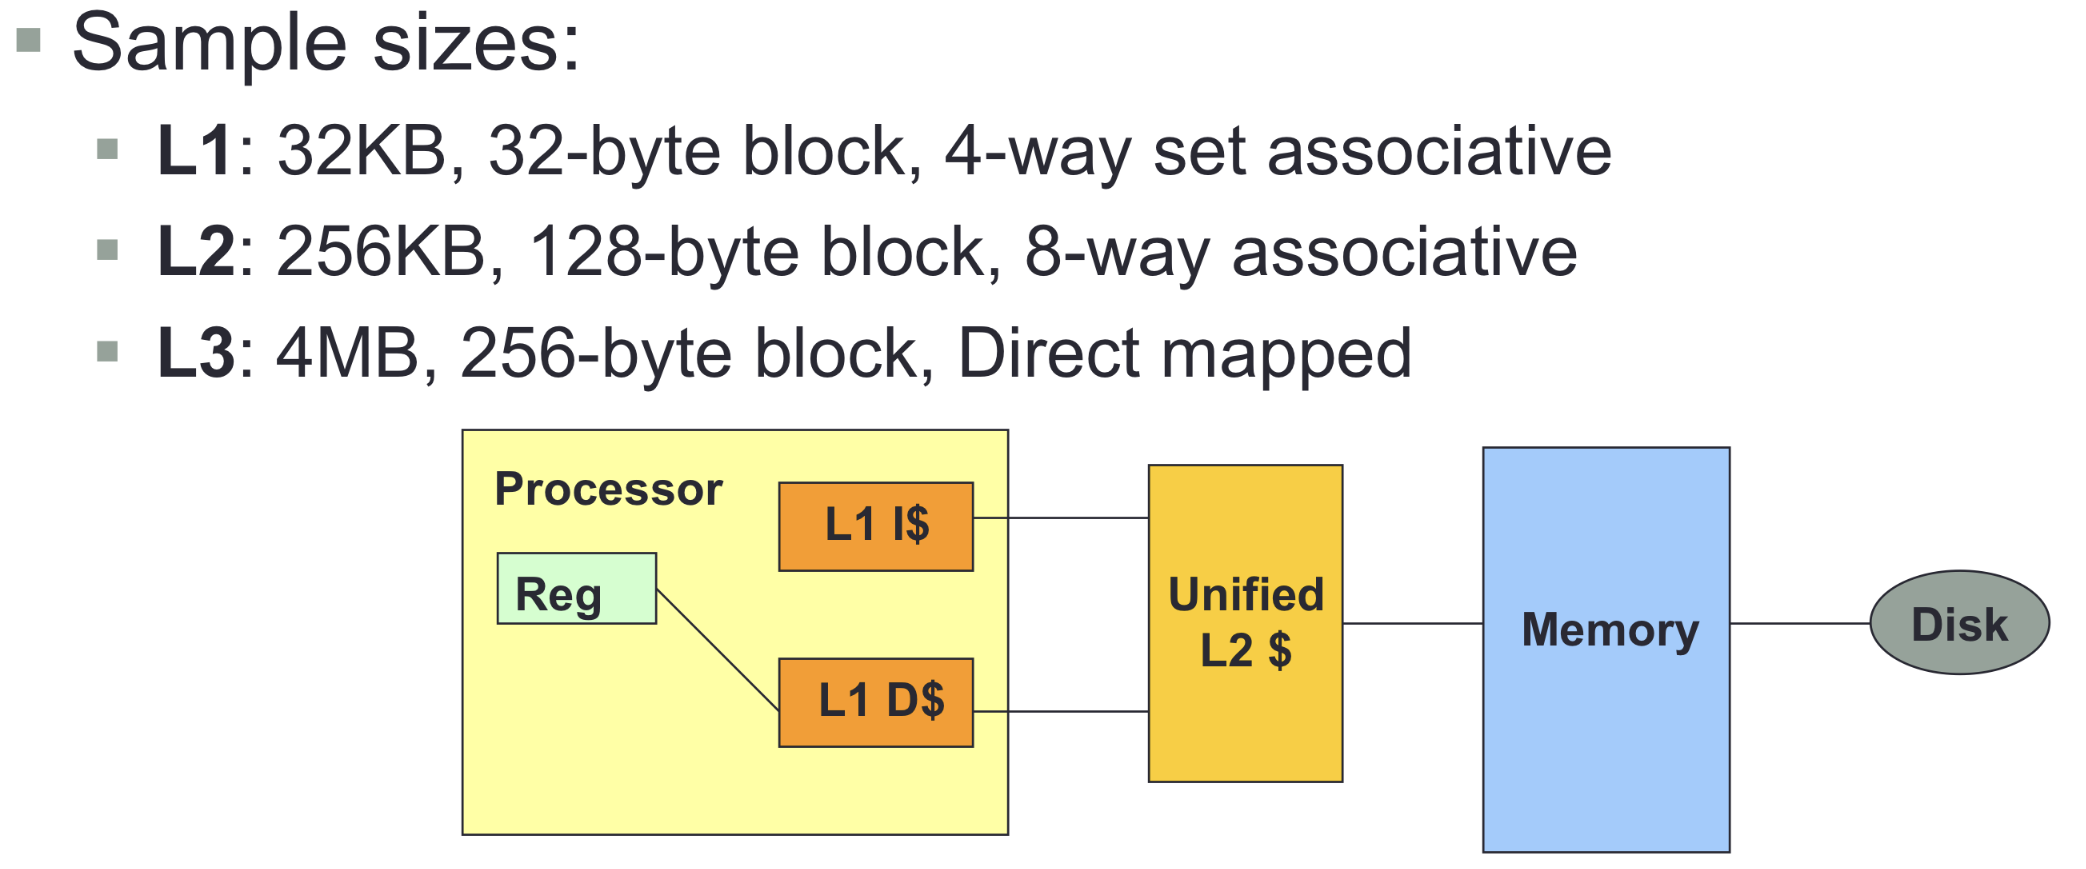
\includegraphics[width=0.7\textwidth]{multilevel}
\end{figure}

\end{document}
